\documentclass[12pt,a4paper,oneside]{book}
%Formattazione e codifica caratteri
\usepackage[english]{babel}
\usepackage[utf8]{inputenc}
\usepackage{microtype}
\usepackage{sansmathfonts}
% Tavola dei contenuti
\usepackage{tocloft}
\renewcommand{\cftdot}{}
\setlength{\cftbeforechapskip}{5pt}
% Figure
\usepackage{graphicx}
\usepackage{caption}
\usepackage{subfig}
\usepackage{svg}
\usepackage{float}
% Matematica
\usepackage{amsmath,amsfonts,amssymb,amsthm}
\usepackage{color}
% Tabelle
\renewcommand*\familydefault{\sfdefault}
\usepackage{booktabs}
%Listati
\usepackage{listings}
\lstloadlanguages{MATLAB}
% Testatine
%\author{A. Siniscalchi}
\usepackage{fancyhdr}
\usepackage{epigraph}
\usepackage{titlesec, blindtext}
\usepackage[dvipsnames]{xcolor}
\usepackage{tikz-network}
\usepackage{pgfplots}
 \pgfplotsset{compat=newest}
  \usetikzlibrary{plotmarks}
  \usetikzlibrary{arrows.meta}
  \usepgfplotslibrary{patchplots}
  \usepackage{grffile}

\usepackage{tikz}
\usepackage{tikz-cd}
\usepackage{hyperref}
\pgfplotsset{plot coordinates/math parser=false}
\pagestyle{fancy}
\setlength{\headheight}{15pt}
\fancyhf{}
\fancyhead[LE,RO]{}
\fancyhead[RE,LO]{\leftmark}
\fancyfoot[CE,CO]{}
\fancyfoot[LE,RO]{\thepage}

\renewcommand{\headrulewidth}{1.5pt}
% Titoli dei capitoli che "rubano" meno spazio

\definecolor{gray75}{gray}{0.75}
\newcommand{\hsp}{\hspace{15pt}}

\SetVertexStyle[MinSize=1\DefaultUnit,FillColor=white]


% Per importare le figure in MATLAB
  \newlength\figureheight
 \newlength\figurewidth
%Per le osservazioni
\theoremstyle{plain}
\newtheorem{thm}{Theorem}[section]
\newtheorem{lem}[thm]{Lemma} 
\newtheorem{obs}[thm]{Observation} 
\newtheorem{prop}[thm]{Proposition}
\newtheorem{cor}[thm]{Corollary} 
\newtheorem{rem}[thm]{Remark}
\newtheorem{ex}[thm]{Example} 
\newtheorem{cla}[thm]{Claim} 
\newtheorem{as}[thm]{Assertion}
\newtheorem{note}[thm]{Note}
\newtheorem{defn}[thm]{Definition}

%COMANDI PERSONALIZZATI 
\newcommand{\Q}{\mathbb{Q}}
\newcommand{\R}{\mathbb{R}}
\newcommand{\B}{\mathbb{B}}
\newcommand{\C}{\mathbb{C}}
\newcommand{\Z}{\mathbb{Z}}
\newcommand{\D}{\mathbb{D}}
\newcommand{\s}{\mathbb{S}}
\newcommand{\torus}{T_{2, 2g+1}}
\newcommand{\tonde}[1]{\left( #1 \right)}
\newcommand{\ses}{\Leftrightarrow} 
\newcommand{\abs}[1]{\left\vert#1\right\vert}
\newcommand{\angol}[1]{\langle #1 \rangle}
\newcommand{\spa}{\mathbin{\textcolor{white}{-}}} 
\newcommand{\q}[1]{``#1''}
\newcommand{\inter}{\nu(K_m)^{\mathrm{o}}}
\newcommand{\interd}{\nu(D')^{\mathrm{o}}}
\newcommand{\estd}{\mathbb{B}^4 \setminus \nu(D)^{\mathrm{o}}}
\newcommand{\estdi}{\mathbb{B}^4 \setminus \nu(D')^{\mathrm{o}}}
\newcommand\restr[2]{{% we make the whole thing an ordinary symbol
  \left.\kern-\nulldelimiterspace % automatically resize the bar with \right
  #1 % the function
  \littletaller % pretend it's a little taller at normal size
  \right|_{#2} % this is the delimiter
  }}
\newcommand{\littletaller}{\mathchoice{\vphantom{\big|}}{}{}{}}

% per mettere le figurelle
%\begin{figure}[h]
    %\centering
    %\includegraphics[scale=0.25]{figures/prova.jpeg}
    %\caption{Caption}
    %\label{fig:evviva ho messo una figura}
%\end{figure}
%faccio riferimento \ref{fig:evviva ho messo una figura}
% Comando per il testo riempitivo: rimuovere prima della fine
%report
\begin{document}
%\usepgfplotslibrary{external} 
%\tikzexternalize[prefix=tikz/]
\titleformat{\chapter}[display]{\large\centering}{CHAPTER \thechapter}{5pt}{\centering\bfseries}[\vskip 15pt]  
\titleformat{\section}[hang]{\normalsize\bfseries}{\thesection.{ }}{0pt}{\centering}[{\vskip 10pt}]
\titleformat{\subsection}[hang]{\normalsize\bfseries}{\thesubsection.{ }}{0pt}{}[{\vskip 5pt}]

\begin{titlepage}
\begin{figure}[t]
	\centering
\includegraphics[width=0.35\textwidth]{figures/stemma_unipi.png}\\[1em]
	{\LARGE \textsc{Università di Pisa}}\\
	\vspace*{-0.5em}\rule{0.6\textwidth}{0.4pt}
\end{figure}
\begin{center}
	\textbf{Dipartimento di Matematica \\ Corso di Laurea Magistrale in Matematica\\}
	\vspace{15mm}
	{\centering Tesi di Laurea Magistrale}\\[1em]
    {\LARGE{\bf On Exotic Symplectic Surfaces \\ in Convex $4$-Manifolds}}\\
	\vspace{3mm}
	
\end{center}

\vspace{36mm}

\begin{minipage}[t]{0.47\textwidth}
	{\large{\bf Relatore:\\Prof. Paolo Lisca \\ \\
     Controrelatore:\\Prof. Carlo Petronio}}
\end{minipage}\hfill
\begin{minipage}[t]{0.47\textwidth}\raggedleft
	{\large{\bf Candidato:\\Alessio Siniscalchi}}
\end{minipage}


\vfill
\centering{\rule{0.5\textwidth}{0.4pt}}\\
\centering{\large{\bf Anno Accademico 2023/2024 }}

\end{titlepage}
\addcontentsline{toc}{chapter}{Abstract}
\chapter*{Abstract}
A pair of smoothly embedded surfaces in a $4$-manifold $X$ is said to be exotic if they are topologically isotopic but not smoothly isotopic. We first describe Hayden's construction of infinitely many pairs of exotic, symplectic ribbon disks in $\B^4$. We then present a simpler example in the topological setting. The construction is explicit, allowing the resulting disks to be drawn by hand. By capping these disks off in larger $4$-manifolds, we obtain infinite pairs of exotic closed surfaces. Finally, we discuss extensions to the higher-genus case.
\addcontentsline{toc}{chapter}{Notations}
\chapter*{Notations}
In the section, we list some common notations used in this thesis. 
\begin{itemize}
\item $X$ denotes a $4$ manifold, since it has a degree $4$ point
\item $Y$ denotes a $3$ manifold, since it has a degree $3$ point
\item $B^4$: the unit $4$ dimensional ball
\item $\s^3$: the boundary of $\B^4$
\item $T_{m, n}$: the torus knot of type $(m, n)$
\item $\nu(K)$: a tubular neighbourhood of a knot
\item $tb(K)$: the Thurston Bennequin number of $K$
\item $Y(K)_{\frac{m}{n}}$: $\frac{m}{n}$-framed surgery along $K$
\item $F \cdot F'$: the intersection number of two embedded surfaces in $X$
\item $Diff(M)$: the set of diffeomorphisms of $M$, up to isotopy
\item $Isom(M)$: the isometry group of a hyperbolic manifold
\item $\xi_{st}$: the standard contact form on $\s^3$
\item $\omega_{st}$: the standard symplectic form on $\R^4$
\item $\mathfrak{L}_v$: the Lie derivative along the vector field $v$
\end{itemize}

\cleardoublepage
\tableofcontents
\addcontentsline{toc}{chapter}{Introduction}
\chapter*{Introduction}
Let $X$ be a smooth $4$-manifold. 
\begin{defn} Two smoothly embedded surfaces $S, S' \subseteq X$ are said to be exotic if they are isotopic through homeomorphisms of $X$ but not through diffeomorphisms of $X$. 
\end{defn}
The study of exotic surfaces is motivated by the following major open question.\\
\\
\textbf{Open Problem} \\
Do exotic, closed, orientable surfaces exist in $\s^4$? \\ \\
Much progress in this area has been driven by questions arising from complex geometry. If $X$ is a simply connected Kahler surface, then two homologous, closed, complex curves are smoothly isotopic. On the other hand, when $X$ is only required to be smooth, then there are examples of infinite families of surfaces that are pairwise exotic. \\ \\
\textbf{Why the Symplectic Setting?} \\
The symplectic setting is balanced between the rigidity of closed complex curves and the flexibility of arbitrary smooth surfaces. Fintushel and Stern constructed some symplectic $4$-manifolds each containing a pair of symplectic surfaces that are homologous but not smoothly isotopic \cite{fintushel1999symplectic}.
The existence of infinitely many pairs of properly embedded exotic, positive genus surfaces in $\B^4$ was independently established by Hayden in \cite{hayden2021exoticallyknotteddiskscomplex} and by Juhàsz, Miller and Zemke in \cite{Juh_sz_2021}. \\ \\
\textbf{Hayden's Contribution} \\
Hayden proved the genus zero case, demonstrating the existence of exotic disks properly embedded in $\B^4$ and exotic spheres in knot traces. In addition, his construction guaranteed that both surfaces are symplectic, whereas in the earlier work, at least one of them is not symplectic.
\\ \\
In this thesis, following the work of Hayden, we construct infinite pairs of exotic, symplectic surfaces properly embedded $\B^4$, with arbitrary genus. \\
A key advantage of Hayden’s approach is its explicit nature, allowing the resulting surfaces to be drawn by hand. Moreover, it applies in both topological and symplectic settings, enabling further exploration of related phenomena. \\
Beyond constructing these exotic surfaces, this thesis compares different strategies for proving exoticness and provides a detailed exposition of Hayden’s techniques, including useful tricks and insights. \\ \\
For the reader's convenience, we outline the structure of this thesis:
\begin{itemize}
\item Chapters 1 \& 2: A review of Kirby calculus and the theory of Stein $4$-manifolds, alongside with the symplectic tools necessary for proving our main theorems.
\item Chapter 3: The construction of infinitely many pairs of exotic (relatively to the boundary), symplectic ribbon disks properly embedded in $\B^4$, alongside with a simpler example in the topological setting. Additionally, we discuss how exotic surfaces yield exotic $4$-manifolds with boundary (see Corollary \ref{giotto}).
\item Chapter 4: The construction of infinitely many pairs of exotic, symplectic spheres in larger convex $4$-manifolds, completing our discussion on the minimal topology setting (i.e. genus-$0$ surfaces).
\item Chapter 5: The extension of these constructions to higher genus surfaces by attaching bands.
\end{itemize}

This thesis includes more than 120 hand-drawn figures to illustrate the constructions and techniques.

\chapter{An Introduction to Kirby Calculus}
This chapter introduces basic notions of Kirby calculus and related topics. For a complete and detailed introduction, we refer the reader to the Gompf and Stipsicz's book \cite{gompf1999four} and Akbulut's book \cite{akbulut2001four}.
Kirby calculus, named after Robion Kirby, is a diagrammatic tool for studying $4$-manifolds.
\section{Anatomy of a $4$-Manifold}
Let $X$ be an orientable, connected $4$-manifold. We assume the reader is familiar with handle decompositions and Morse functions. For an introduction, consult \cite{benedetti2019lectures}. \\
Consider an ordered handle decomposition of $X$. Since $X$ is connected, handle cancellation ensures we can reduce the handle decomposition to include only one $0$-handle. Applying the same procedure to the dual handle decomposition results in a handle decomposition with only one $0$-handle and one $4$-handle.
Denoting by $n_i$ the number of $i$-handles $i=0,\dots 4$, we write: $$
X = H_0 \cup H_1^1 \cup \dots \cup H_1^{n_1}\cup H_2^1
\cup\dots\cup H_2^{n_2}\cup H_3^1\cup \dots \cup H_3^{n_3} \cup H_4$$
Our strategy involves drawing the attaching region schematically. Start with $1$-handles $H_1 = \D^0 \times \D^4$, which are attached to $$
\partial \D^4 = \s^3 = \R^3 \cup \{\infty\}
$$
The attaching region is $\s^0 \times \D^3 = \{-1, 1\}\times \D^3$.
There is a unique way to attach them to make the resulting manifold orientable.
We remove two balls from $\R^3$, and we identify their boundaries through a reflection. We represent the whole attaching region, as in Figure \ref{fig:kiuby}(a).
Observe that $$
H_0 \cup H_1^1 \cup \dots \cup H_1^{n_1} = \natural_1^{n_1}(\s^1 \times \D^3)
$$After all the $1$-handles are attached, the resulting boundary becomes: $$Y = \#_1^{n_1}(\s^1 \times \s^2)$$
The attaching spheres of the $2$-handles form a link $L$ in $Y$. To describe the $2$-handle attachment, we use framings. Since every $3$ manifold is parallelizable, \cite{benedetti2019lectures}, we can arbitrarily choose a trivialization of $\nu(L)$. After this choice, the trivializations of $\nu(L) \cong L \times \D^2$ are classified by $$
\pi_1(O(2)) \cong \Z
$$Each component of $L$ is assigned an integer, specifying the framing. Figure \ref{fig:kiuby}(b) is an example of a Kirby diagram.
\begin{figure}[H]
    \centering
    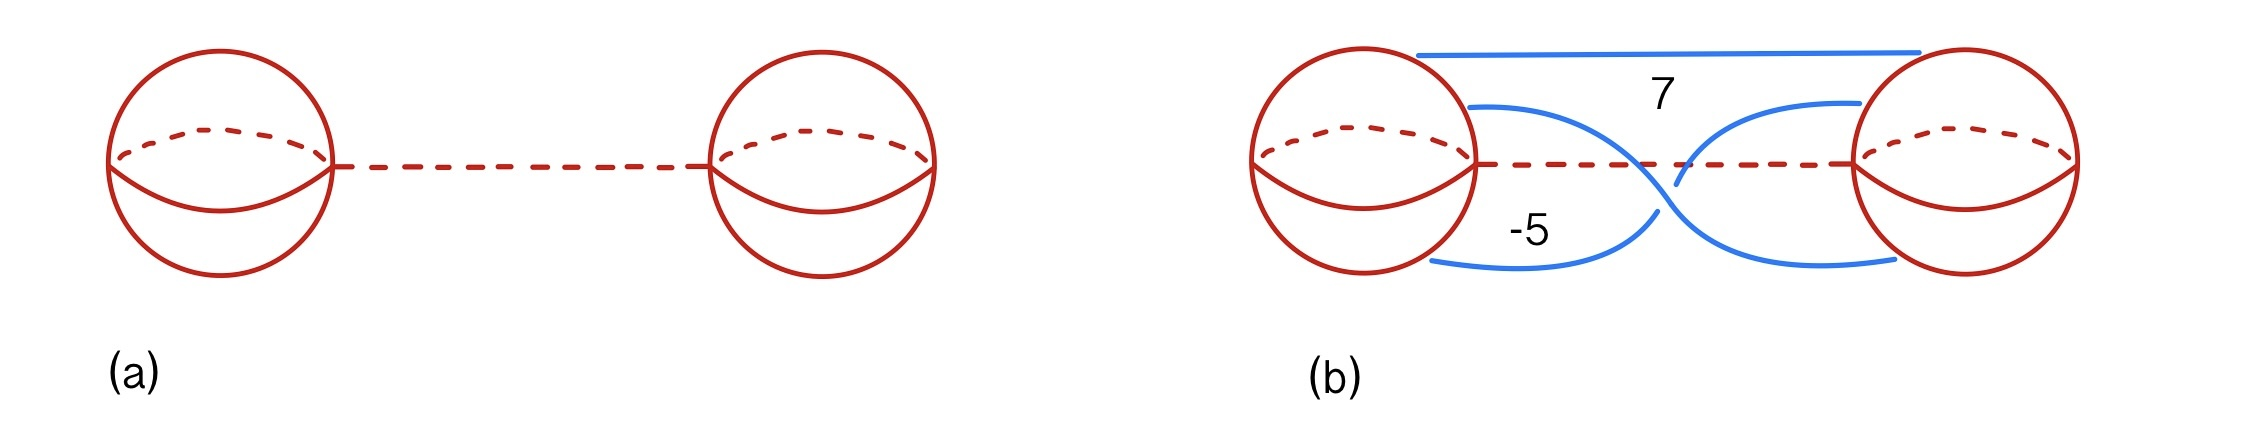
\includegraphics[scale=0.2]{figures/kiuby.jpeg}
    \caption{A $1$-handle on the left, a Kirby diagram on the right}
    \label{fig:kiuby}
\end{figure}
\begin{cla}
If $X$ is closed, the attachment of $3$-handles is immaterial.
\end{cla}
Indeed, examining the dual handle decomposition, we find $$
\partial (\B^4 \cup_1^{n_1} H_1^i \cup_1^{n_2} H_2^j) = \#_1^{n_3}(\s^1 \times \s^2)
$$and $n_3 = n_1$. 
\begin{thm}(Laudenbach, Poenaru) \\
Every self diffeomorphism of $\#_1^k(\s^1 \times \s^2)$ extends to a self diffeomorphism of $\natural_1^k(\s^1 \times \D^3)$
\end{thm}
As a result, there is a unique way to finish building $X$ from $(\B^4 \cup_1^{n_1} H_1^i \cup_1^{n_2} H_2^j)$, by attaching $3$ and $4$-handles.
\section{Drilling out Disks}\label{driii}
In this section, we introduce Akbulut's notation for $1$-handles, called the dotted circle notation. While doing that, we explain how to find the Kirby diagram of a unknotted disk complement in $\B^4$. \\ \\
Consider $X \cup H_1$. If $X$ is connected, we can recover $X$ by gluing a $2$-handle. Then, we can dismantle the $2$-handle by carving a disk, that means drilling out a open tubular neighbourhood of a properly embedded disk.
As a result, attaching a $1$-handle to $\B^4$, is the same as removing a disk
$D$ from $\B^4$, with $\partial D \subseteq \s^3$.
This allows us to represent a $1$-handle as a boundary of the carved disk, marked with a dot\footnote{This is only to distinguish $1$ and $2$-handles}. 

\section{Kirby Moves}
After introducing the combinatorial objects, which are Kirby diagrams, we proceed by introducing a set of moves, called Kirby moves. We translate the well known moves on handle decompositions, into the language of Kirby diagrams. For convenience, we use Akbulut's notation.  \\ 
\textbf{1-handle slide}: 
We slide a $1$-handle over the other, as in Figure \ref{fig:hs1}.
\begin{figure}[H]
    \centering
    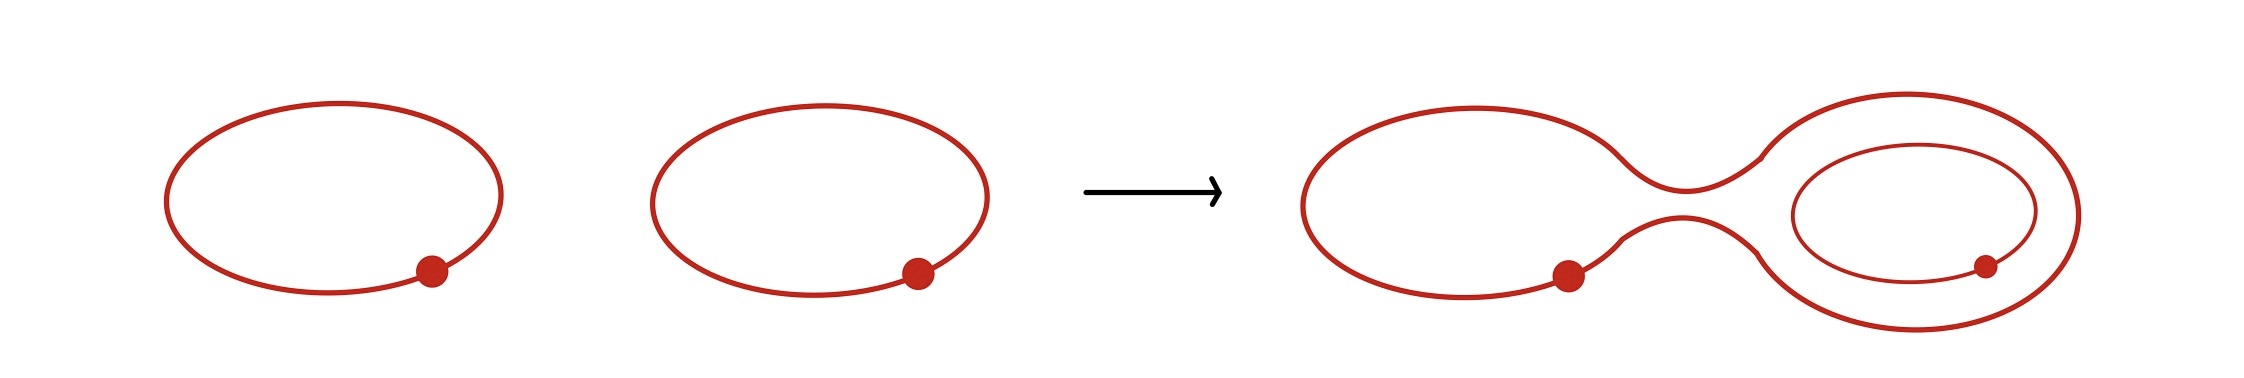
\includegraphics[scale=0.2]{figures/hs1.jpeg}
    \caption{A $1$-handle slide}
    \label{fig:hs1}
\end{figure}
\textbf{2-handle slide}:
Suppose we want to slide $K_1$ over $K_2$. We consider a parallel copy $K_2'$ of $K_2$ and then we perform the connect sum $K_1 \#K_2'$. The new framing on $K_2$ is: $$
f_{K_1}+f_{K_2} + 2lk(K_1, K_2)
$$
\begin{figure}[H]
    \centering
    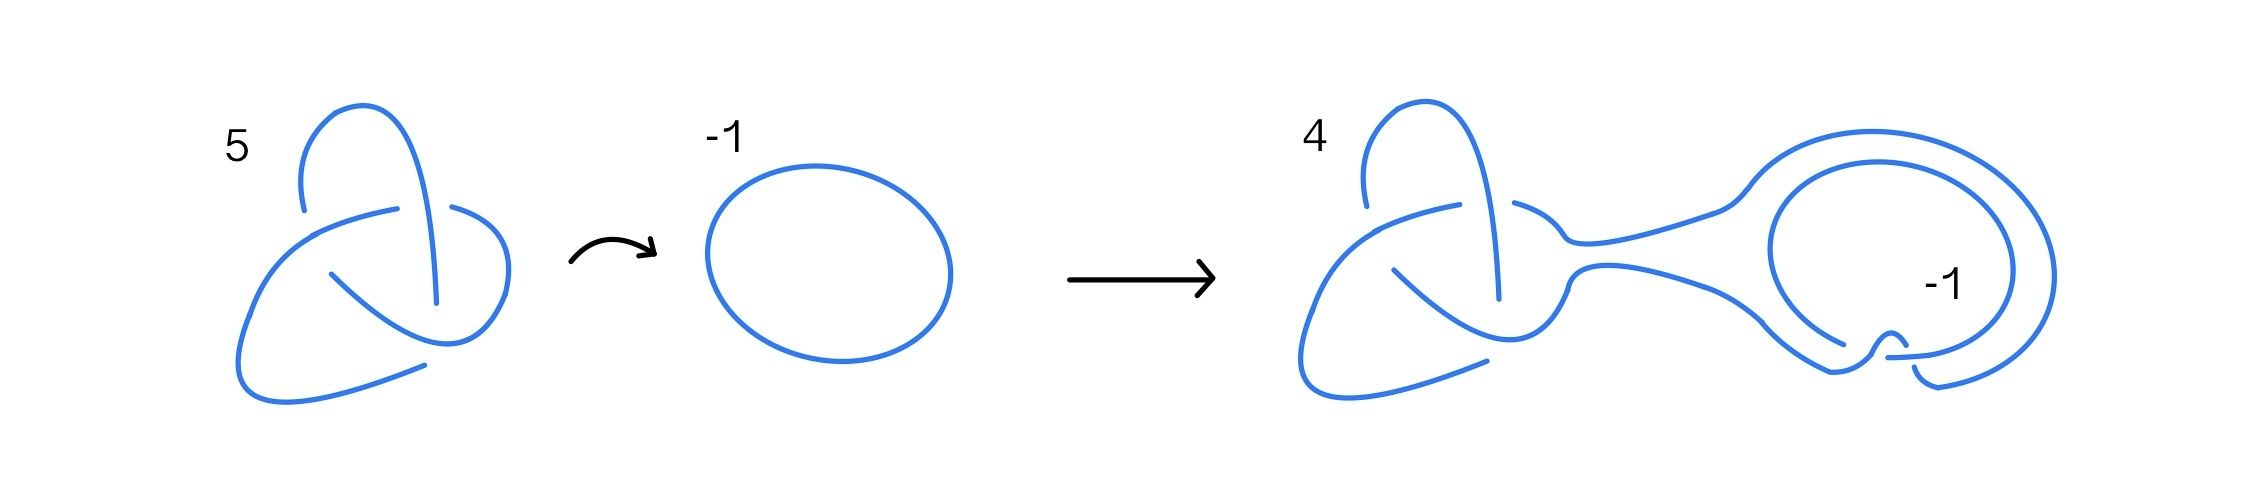
\includegraphics[scale=0.2]{figures/hs2.jpeg}
    \caption{A $2$-handle slide}
    \label{fig:hs2}
\end{figure}
\textbf{Handle creation and cancellation of complementary pairs}: \\
Suppose that the attaching sphere of a $2$-handle transversally intersects the belt sphere of a $1$-handle in one point. Then we can perform a handle cancellation. Its inverse is called handle creation. \\
These moves don't change the manifold represented by a Kirby diagram, up to diffeomorphisms. Moreover the following theorem holds.
\begin{thm} Let $X$ be a closed $4$-manifold. Any two Kirby diagrams of $X$ are related by a finite sequence of isotopies and Kirby moves. 
\end{thm}
\section{The Light Bulb Trick}
In the next chapters, we manipulate knots and core curves inside Kirby diagrams. In particular, it will be useful to unlink a knot $K$ from the attaching curve of a $2$-handle. \\ \\
If such a core curve is a $0$-framed unlink, then we just perform a number of handle slides for each time $K$ passes through the blue circle, as depicted in Figure \ref{fig:squish}.
\begin{figure}[H]
    \centering
    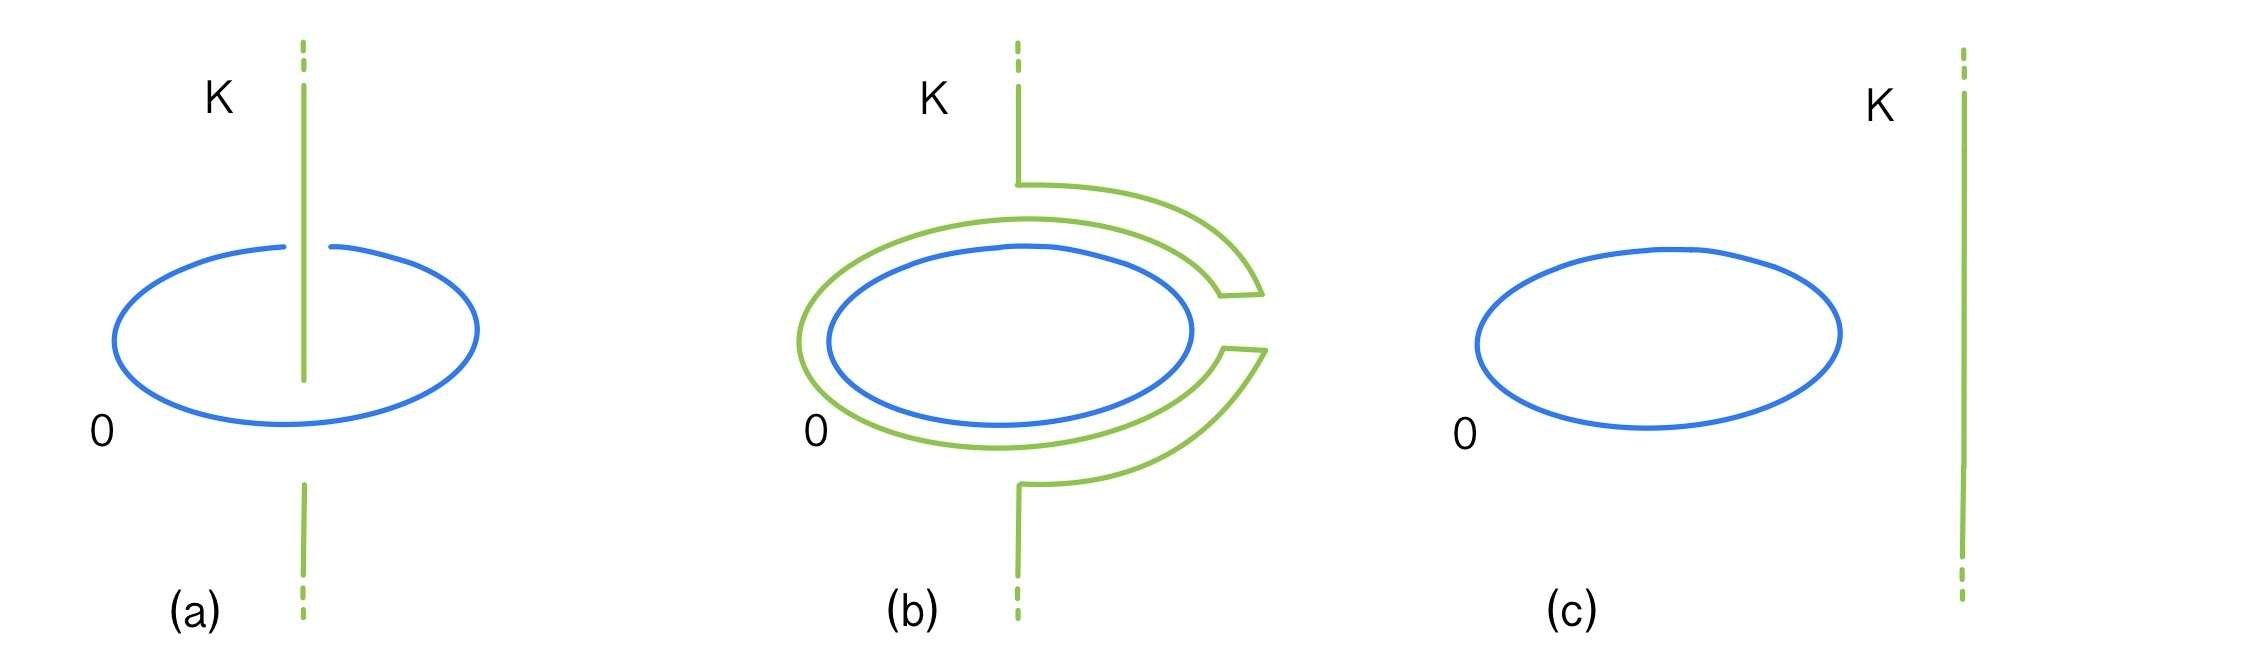
\includegraphics[scale=0.2]{figures/squish.jpeg}
    \caption{Unlinking $K$ from a $0$-framed $2$-handle}
    \label{fig:squish}
\end{figure}
When the $2$-handle is knotted, then the problem could get way harder. However, if $K$ transversely intersects the core of the $2$-handle in one point, then the light bulb trick comes in clutch.
\begin{thm}Let $K \subseteq \s^1 \times \s^2$ be a knot intersecting $\{x\} \times \s^2$ transversely in one point $(x, y)$. Then $K$ is isotopic to $\s^1 \times \{y\}$ via an isotopy fixing $\{x\}\times \s^2$.
\end{thm}
\begin{ex}
The following figure shows how to undo a crossing. The main idea is to slide a piece of knot all the way down to the sphere and then send it back up.
\end{ex}
\begin{figure}[H]
    \centering
    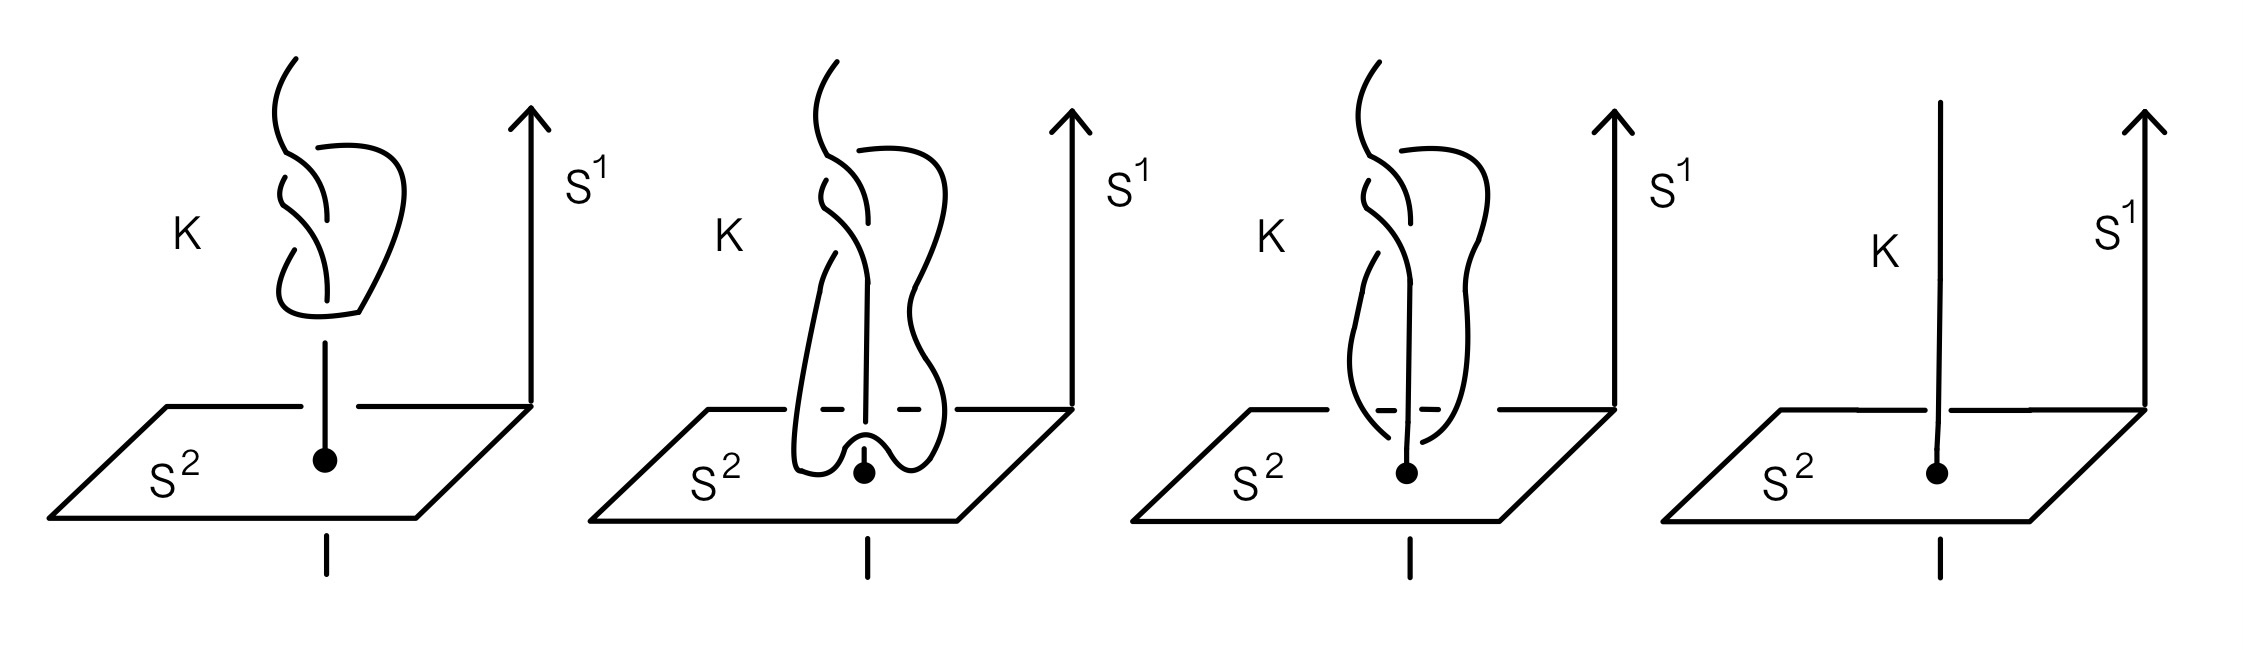
\includegraphics[scale=0.2]{figures/lbt.jpeg}
    \caption{Light bulb trick}
    \label{fig:lbt}
\end{figure}
\section{Ribbon Disks Complement}\label{acqua}
In this section, we outline an algorithm to find the Kirby diagram of a ribbon disk exterior in $\B^4$. We recall the definition for context.
\begin{defn}A disk embedded in $\B^4$ is ribbon if it has no local maxima with respect to the radial height.
\end{defn}
Thus we can visualize a ribbon disk as a finite collection of unknotted disks with some bands attached. \\
Let $K \subseteq \s^3$ be a ribbon knot bounding $D$. 
By performing ribbon moves (band surgeries), we turn $K$ into a collection of disjoint unknotted circles $\{C_i\}_{i=1}^k$ which bound (unknotted) disks $\{D_i\}_{i=1}^k$. For $i = 1 \dots k$, we carve out $D_i$ by placing a dot on $C_i$, as discussed in section \ref{driii}.
\begin{obs}The inverse of the ribbon moves define a cobordism between $\#_1^k(\s^1 \times \s^2)$ and $\s^3 \setminus K$.
\end{obs}
 Each time a circle is merged with another, it creates a $0$-framed $2$-handle in $\B^4 \setminus D$, attached as in Figure \ref{fig:carve}(c) \cite{akbulut2001four}.
\begin{figure}[H]
    \centering
    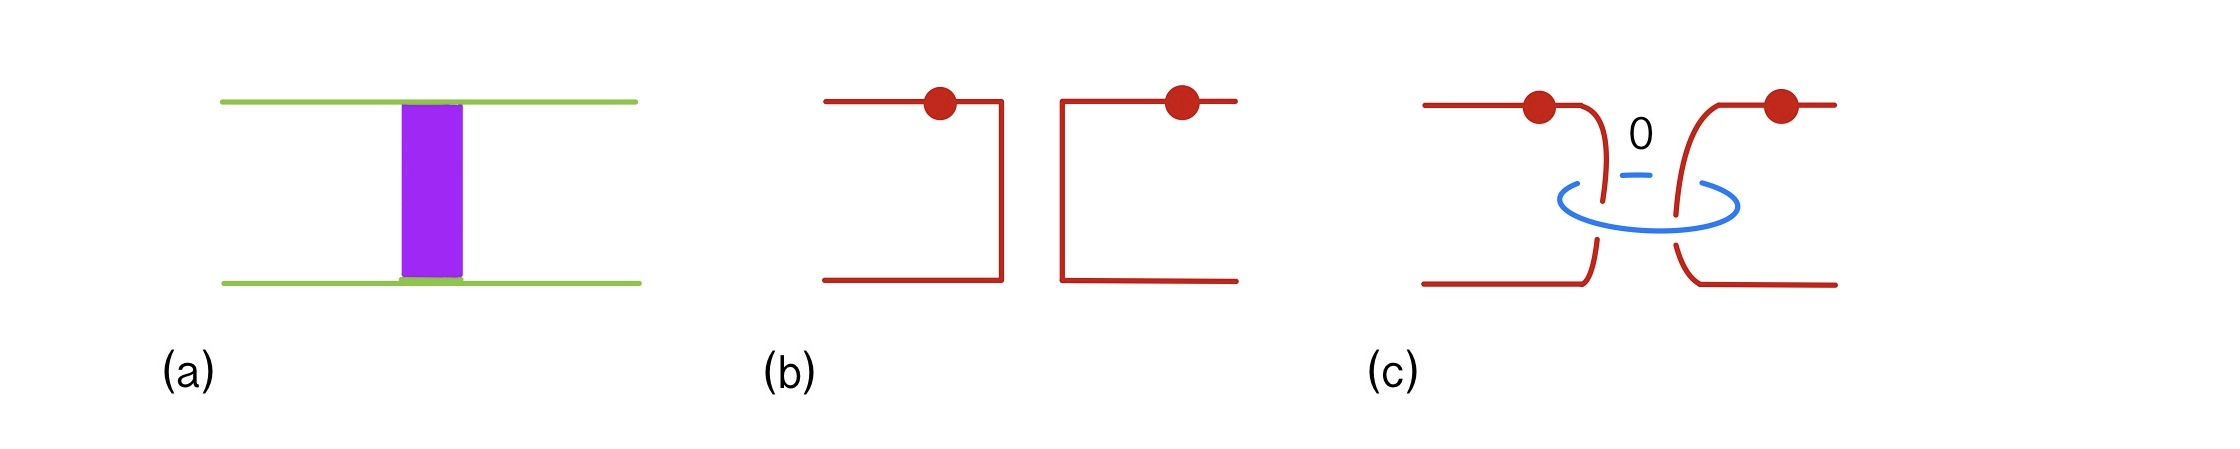
\includegraphics[scale=0.2]{figures/carve.jpeg}
    \caption{Carving a ribbon disk}
    \label{fig:carve}
\end{figure}
\section{A Recipe to Compute the Fundamental Group}\label{rec}
Let $\mathfrak{k}$ be a Kirby diagram of $X$. In this section we describe a procedure to compute the fundamental group of $X$ from $\mathfrak{k}$.
It is well known that a handle decomposition carries a CW complex structure. Collapsing a $k$ handle $\D^k \times \D^{n-k}$ onto the core $\D^k \times 0$, gives rise to a $k$ cell \cite{benedetti2019lectures}. 
\begin{ex}Let $X = \B^4 \cup_1^{n_1}H_1^i$ Then $$
X \sim \vee_1^{n_1} \s^1
$$where each $S^1$ is the core of a $1$-handle. 
\end{ex}
Now we explain how to obtain a presentation of $\pi_1(X)$. For more details, we refer the reader to \cite{saveliev2012}.
\begin{rem}
In general $\pi_1(X)$ is determined by the union of handles of index $\leq 2$.
\end{rem}
\textbf{Procedure}: 
\begin{itemize}
    \item Choose orientations on the attaching spheres,
    \item The generators are the $1$-handles represented as core curves,
    \item The relations are specified by the oriented attaching $\s^1$ of the $2$-handles, written as words of the generators (up to homotopy).
\end{itemize}
\begin{rem}The framing coefficients of the $2$-handles are immaterial.
\end{rem}
We provide two examples, one of which involves the dotted circle notation.
\begin{ex}
\begin{figure}[H]
    \centering
    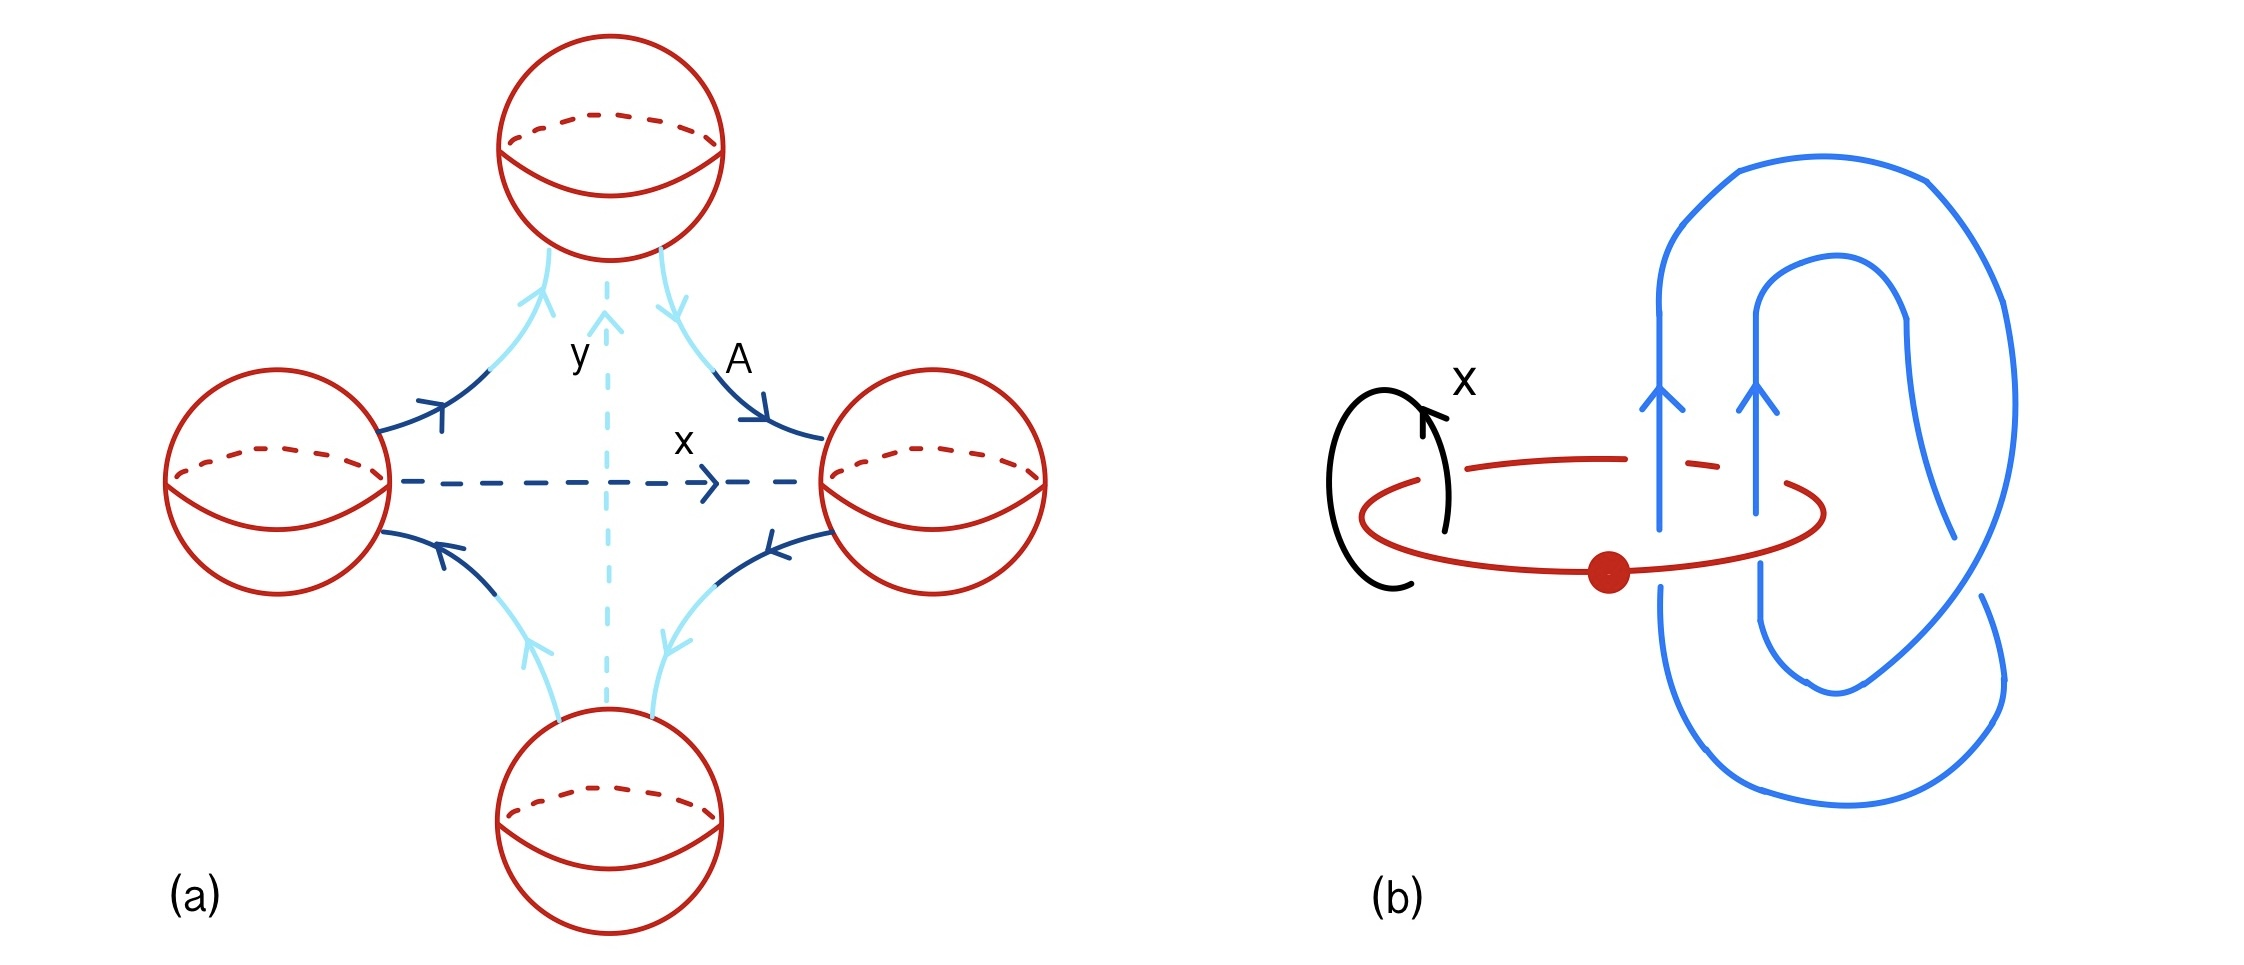
\includegraphics[scale=0.2]{figures/ex_pi1.jpeg}
    \caption{Fundamental group computation}
    \label{fig:funda}
\end{figure}
Consider Figure \ref{fig:funda}(a). Starting from the point A, we obtain the following presentation : $$
\pi_1(X) = \langle x, y \quad | \quad xyx^{-1}y^{-1} \rangle \cong \Z \oplus \Z
$$
Whereas from the diagram \ref{fig:funda}(b), we deduce the following presentation: $$
\pi_1(X) = \langle x \quad | \quad x^2 \rangle = \Z/2\Z
$$
\end{ex}
\section{A Glance at Double Branched Covers}\label{covers}
In this section we prove the existence and uniqueness of the double branched cover of $\B^4$ along an embedded disk $D$, then we sketch an algorithm to draw its Kirby diagram. \\ \\
We recall the general definition for context. Let $M$ be a $4$-manifold.
\begin{defn}
A double branched covering is a proper map $f :N \rightarrow M$ with critical set $B$, called the branch locus, such that:  \\
(i) $f|_{N \setminus f^{-1}(B)} : N \setminus f^{-1}(B) \rightarrow M \setminus B$
is a double covering. \\
(ii) On $f^{-1}(B)$, $f$ is locally defined as $$
\C \times \R_{+}^2 \rightarrow \C \times \R_{+}^2
$$ $$ (z, x) \rightarrow (z^2, x)
$$
\end{defn}
We examine the basic example where $M = \B^4$ and $B$ is an embedded ribbon disk. 
The same techniques apply in similar settings.
\begin{lem} $H_1(\B^4\setminus D) \cong \Z$
\end{lem}
\proof
Consider a open tubular neighbourhood $\nu(D) \cong D \times \B^2$. By Mayer Vietoris' exact sequence, we have: $$
\begin{tikzcd}
0 \arrow[r] & H_1(\nu(D) \setminus D) \arrow[r] & H_1(\B^4 \setminus D)\oplus H_1(\nu(D)) \arrow[r] & 0
\end{tikzcd}
$$
Therefore $H_1(\B^4 \setminus D)\cong \Z$, as desired.
\endproof
By Hurewicz theorem, there exists a surjective homomorphism $\pi_1(\B^4\setminus D) \rightarrow H_1(B^4\setminus D) \cong \Z$. Thus, there exists a unique index $2$ subgroup of $\pi_1(\B^4 \setminus D)$.
This proves the existence and uniqueness of the double covering of $\B^4 \setminus D$. 
Then we locally extend such double covering near the branch locus, in a way that satisfies the local property. The uniqueness of the latter extension follows from the topological fact that a $\s^1$ bundle can be uniquely filled by a $\D^2$ bundle. \\ We denote the double branched covering of $\B^4$ along $D$ as $\Sigma(\B^4, D)$.
\\ 
In section \ref{buffet}, we outline a strategy to draw a Kirby diagram for $\Sigma(\B^4, D)$, providing a concrete example.
\chapter{Stein $4$-Manifolds and Symplectic Tools}
We assume the reader is familiar with the basic concepts of contact and symplectic geometry. For an introduction, consult \cite{geiges2008contact}. 
\section{Fundamental Definitions and Properties}
We begin with the definitions and fundamental properties of Stein $4$-manifolds. 
For an in-depth discussion, we refer the reader to \cite{eliashberg2012stein}.
Let $J$ denote a complex structure on a $4$-manifold $W$.
\begin{defn}
A $J$-holomorphic disk is an embedded disk $$
h : \D^2 \rightarrow W
$$
such that 
$$ dh \circ I = J \circ dh
$$
where $I$ is the natural complex structure on $\D^2 \subseteq \mathbb{C}$.
\end{defn}
\begin{defn}
A strictly $J$-convex function is a strictly subharmonic map when restricted to $J$-holomorphic disks. 
\end{defn}
\begin{defn}
A Stein $4$-manifold is a quadruple $(W, \partial W, J, \phi)$, where: \\
(i) $W$ is a $4$-manifold with $\partial W \neq \emptyset$, \\
(ii) $J$ is a complex structure on $W$, \\
(iii) $\phi : W \rightarrow \R$ is a proper, strictly $J$-convex Morse function, \\
(iv) $\partial W = \phi^{-1}(1)$
\end{defn}
Let $c \in \R$ be a regular value of $\phi$. Set $Y_c = \phi^{-1}(c)$.
\begin{defn}
$Y_c$ is called a Stein fillable $3$ manifold. Moreover $$\{x \in W \quad | \quad \phi(x) \leq c \}$$
is a Stein filling of $Y_c$. 
\end{defn}
The following proposition summarizes some basic facts (straightforward from definitions).
\begin{prop} Using the notation above, we have: \\
(i) $Y_c$ canonically inherits a contact structure given by: $$
TY_c \cap JTY_c
$$
In particular, the boundary carries a canonical contact structure given by:
$$
T\partial W \cap J T \partial W
$$
(ii) $\omega_{\phi} = -dd^{\C}\phi$ is a symplectic $2$ form, thus $W$ is a symplectic $4$-manifold. \\
(iii) $W$ is naturally equipped with the Kahler metric: $$
g(u, v) = \omega(u, Jv)
$$
\end{prop}
\begin{ex} The basic example is $\B^4 \subseteq \C^2$ equipped with the radial height, which is a $J$-convex function. In this case, $\omega_{\phi}$ coincides with $\omega_{st}$.
\end{ex}
We conclude this section with a Theorem due to Lisca and Matic, which provides an obstruction to the existence of certain spheres, in Stein $4$-manifolds. 
\begin{prop}\label{ostruzione} 
Let $W$ be a Stein $4$-manifold. Then $W$ does not admit embedded spheres $S$ in $W \setminus \partial W$ such that $$
S \cdot S = -1
$$
For a proof, we refer the reader to the original article \cite{lisca-matic}.
\end{prop}
\section{Gompf's Standard Form}\label{gom}
We begin this section by stating Eliashberg's characterization theorem, a fundamental result on Stein manifolds.
\begin{thm}\label{el}(Eliashberg's characterization of Stein $4$-manifolds)\cite{eliashberg1990topological}\cite{gompf1998handlebody} \\
Let $X$ be a compact, connected, oriented, $4$-manifold. $X$ admits a Stein structure, if and only if there exist a handle decomposition $$
\B^4 \cup H_1^1 \cup \dots \cup H^{n_1}_1 \cup H_2^1 \cup \dots \cup H_2^{n_2}
$$which satisfies the following conditions: \\
(i) For each $i= 1 \dots n_1$, $H_1^i$ are $1$-handles, \\
(ii) For each $j= 1 \dots n_2$, $H_2^j$ are $2$ handles, \\
(iii) For each $j$ there exist a Legendrian knot $K_j$ in the contact structure induced\footnote{This is determined by the special case $n_2=0$ of the Theorem.} on $$
\partial(\B^4 \cup H_1^1 \cup \dots \cup H^{n_1}_1) \cong \#_1^{n_1}(\s^1 \times \s^2)
$$
and $H_2^j$ is attached along $K_j$, with framing $$
tb(K_j) - 1.
$$
\end{thm}
Gompf, in his work \cite{gompf1998handlebody}, introduced a standard form for Legendrian links in $\#_1^n(\s^1 \times \s^2)$. The main purpose is to provide a convenient way to compute the Thurston-Bennequin invariant. As a result, it will facilitate the application of Eliashberg's theorem.
\begin{defn}A Legendrian link in standard form is described by: \\
(i) A rectangular box in $\R^2$, \\
(ii) A collection of $n \geq0$ pairs of balls, \\
(iii) A front projection of a Legendrian tangle, \\
(iv) A collection of segments, aligned horizontally, and joining the endpoints of the tangle with the balls.
\end{defn}
\begin{figure}[H]
    \centering
    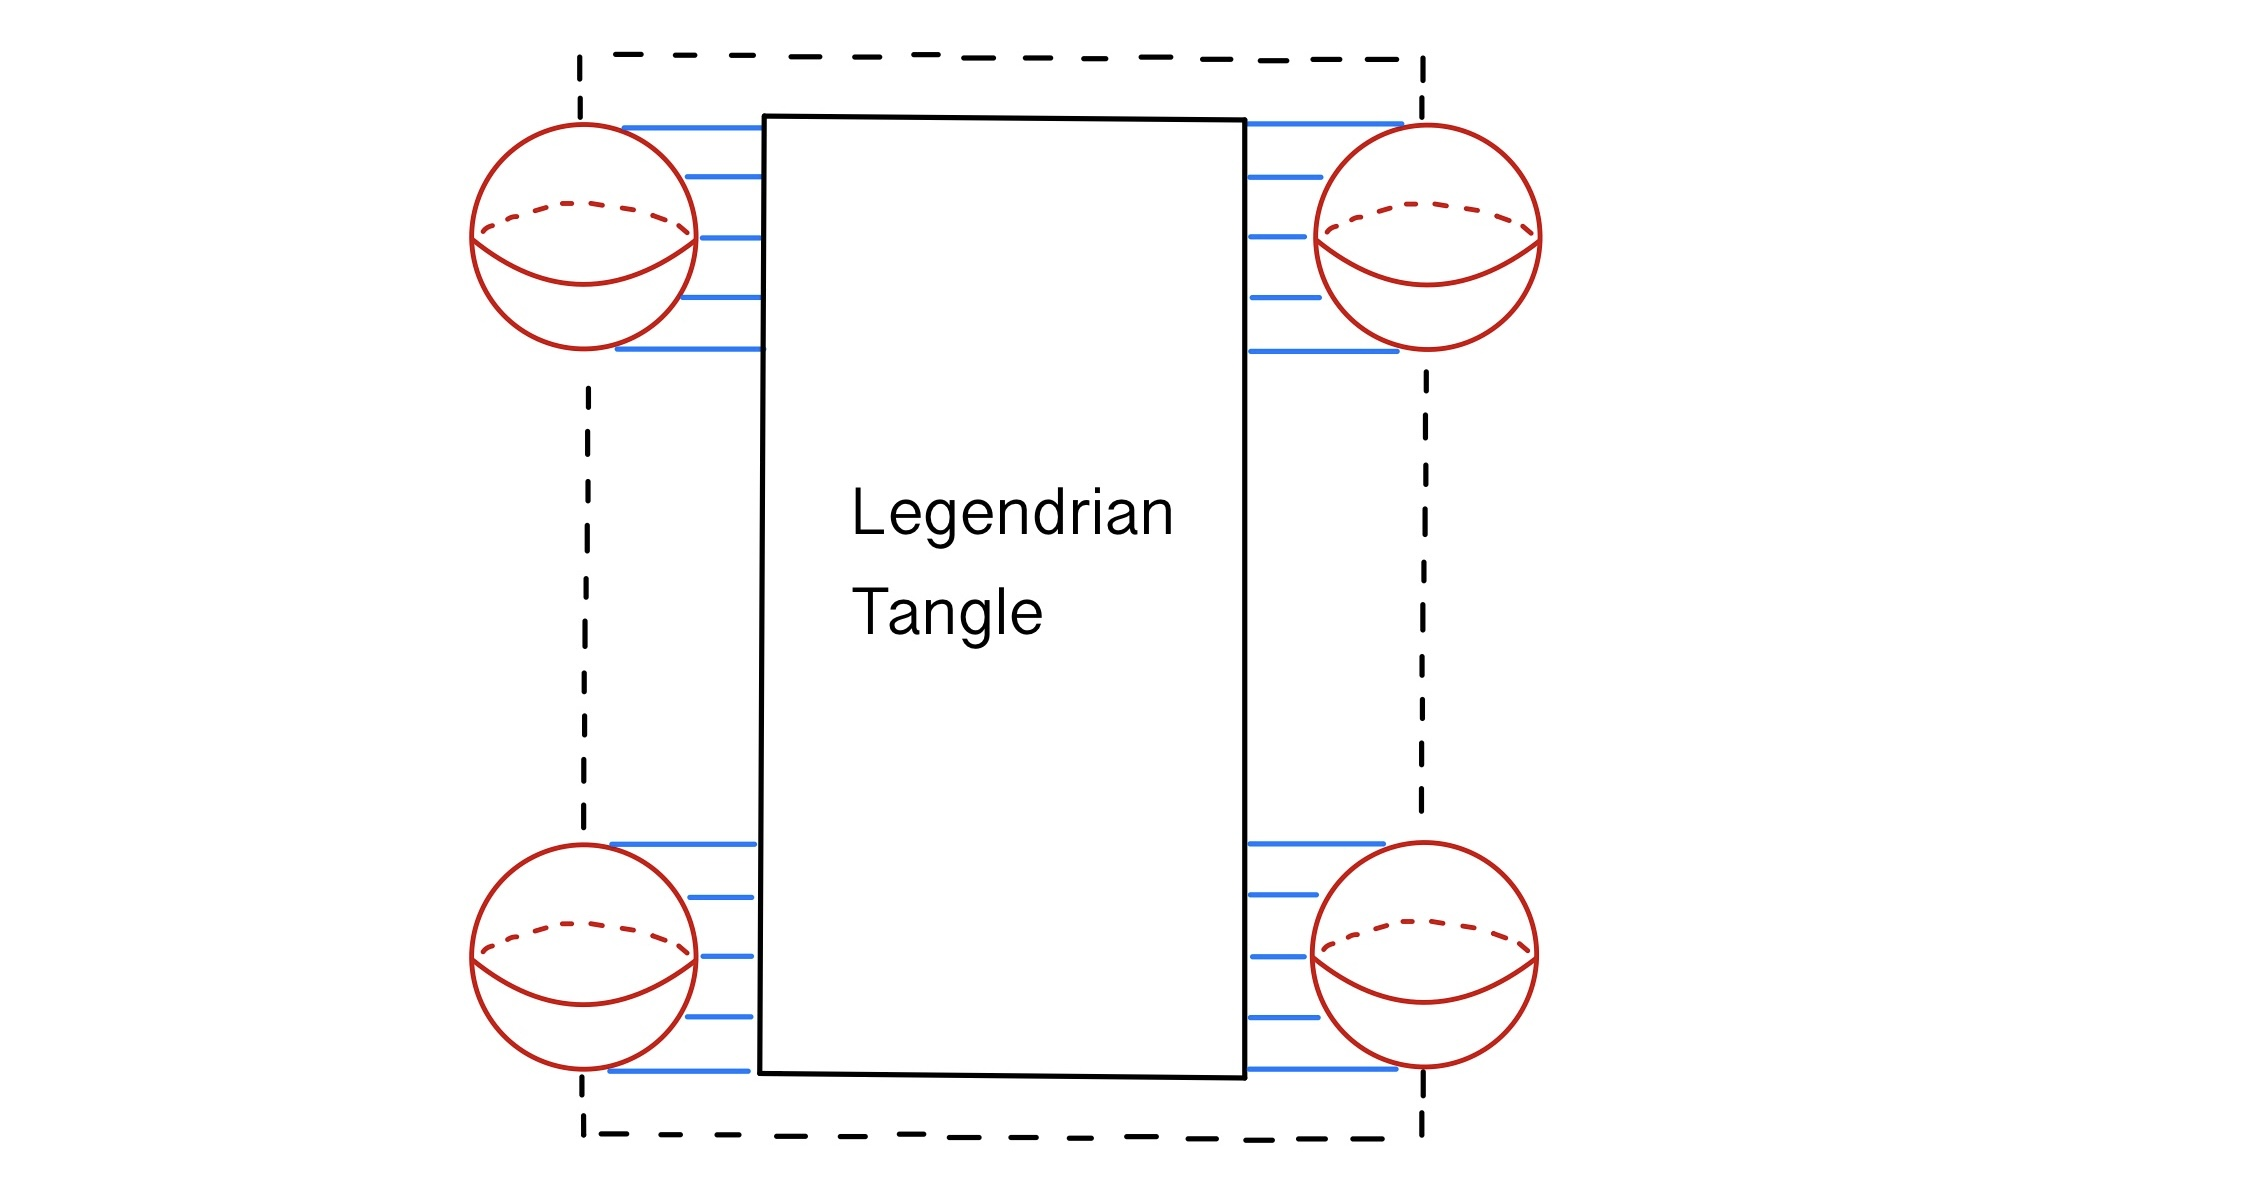
\includegraphics[scale=0.2]{figures/tango.jpeg}
    \caption{A Legendrian link in Gompf's standard form}
    \label{fig:tango}
\end{figure}
This represents a Legendrian link in $\#_1^n(\s^1 \times \s^2)$, after the $1$-handle attachment. 
We need to establish a convention to identify the framings with integers. By gluing the vertical edges of the box, the tangle becomes a link projected in the plane. Therefore, we can define the blackboard framing in the natural way. \\ Gompf shows that the well known formula for the Thurston-Bennequin invariant
$$
tb(K) = w(K)- \# \{\text{right cusps}\}
$$
is well defined for tangles in standard form, and coincides with the integer representing the contact framing \footnote{With respect to the canonical contact structure of $\#_1^n(\s^1 \times \s^2)$, determined by Eliashberg's theorem}.
Moreover, every link in $\#_1^n(\s^1 \times \s^2)$, is contact isotopic to a link in standard form. 
\begin{thm}A compact, connected $4$-manifold is Stein, if and only if, it admits a handlebody decomposition in standard form, with each $2$-handle $H_2^i$ attached to the $i^{th}$ link component $L_i$ with framing $tb(L_i)-1$.
\end{thm}


\section{Comparing Three Notions of Fillability}
In this section, we introduce three notions of symplectic fillability. They are the symplectic analogues of Stein fillability, which is the most powerful type of fillability that can be achieved.
\begin{defn}Let $(Y, \xi)$ be a contact $3$ manifold. \\
(A) $(X, \omega)$ is a weakly symplectic filling of $(Y, \xi)$ if $Y$ is the oriented \footnote{With the orientations inherited from the contact and symplectic structures} boundary of $X$ and $\omega|_{\xi}>0$. \\
(B) $(X, \omega)$ is a strongly symplectic filling of $(Y, \xi)$ if $Y$ is the oriented boundary of $X$, and there exists a contact form $\alpha$ for $\xi$, such that $\omega|_Y = d\alpha$. \\
(C) $(X, \omega)$ is said to be convex if $X$ admits a vector field $v$ that is transversely pointing outward to the boundary and Liouville, i.e. $$
\mathfrak{L}_v\omega = \omega
$$
\end{defn}
Condition (B) is clearly stronger than (A).
\begin{obs}(C) is stronger than (B). 
\end{obs}
In fact, by Cartan's formula, we have: $$
\mathfrak{L}_v\omega = d \iota_v \omega = \omega
$$ by which we can define $\alpha = \iota_v\omega$.
In general, for higher dimensional manifolds, the converse is false. However, in dimension $3/4$, one can extend a generic contact vector field transversely to the boundary, to obtain the desired Liouville vector field. For a complete discussion consult \cite{etnyre1998symplectic}, cfr \cite{Etnyre_2004}.
\begin{ex}$(\B^4, \omega_{st})$ is a convex symplectic manifold, with a Liouville vector field: $$
v = \frac{1}{2}(x\frac{\partial}{\partial x} + y\frac{\partial}{\partial y} +z\frac{\partial}{\partial z} + t\frac{\partial}{\partial t})
$$
\end{ex}
When the $3$ manifold is a homology 3-sphere, weak and strong fillability are equivalent conditions.
\begin{prop}\cite{oo:simple}\label{osha}
Let $(X, \omega)$ be a weakly symplectic filling of $(Y, \xi)$. Suppose that $\partial X = Y$ is a homology $3$ sphere. Then $\omega$ can be modified, with a small perturbation, to be a symplectic form of a strongly symplectic filling of $Y$.
\end{prop}










\chapter{Building Exotic, Symplectic, Ribbon Disks in $\B^4$}
This chapter is devoted to proving the following theorem. 
\begin{thm}\label{prince}
There exist infinitely many transverse knots in $(\s^3, \xi_{st})$, such that each bounds a pair of exotic, symplectic, ribbon disks embedded in $(\B^4, \omega_{st})$.
\end{thm}
\section{A Machinery for Creating Ribbon Disks}
Hayden, in \cite{hayden2021exoticallyknotteddiskscomplex}, invented a method to produce pairs of ribbon disks with the same boundary. This construction is purely topologic.
Let $$ L = A \cup B \cup C
$$be a three component link.
\begin{defn}$L$ is a  quasi Brunnian link if \\
(i) $A, B$ and $C$ are unknots (viewed individually), \\
(ii) $A\cup B$ is a Hopf link, \\
(iii) both $A \cup C$ and $B \cup C$ are unlinks.
\end{defn}
As a first example to illustrate the construction, consider the diagram in Figure \ref{fig:abc}, which appears in \cite{hayden2023brunnianexoticsurfacelinks}. 
\begin{figure}[H]
    \centering
    
\includegraphics[scale=0.2]{figures/abc.jpeg}
    \caption{A quasi Brunnian link}
    \label{fig:abc}
\end{figure}
Removing $C$ turns the diagram into a Hopf link. \\
Decorate $A$ with a red dot and assign the integer $0$ to $B$. Then, we can view $\mathfrak{K} = A \cup B$ as a kirby diagram with the dotted circle notation, as depicted in Figure \ref{fig:trecolori}(a).
\begin{figure}[H]
    \centering
    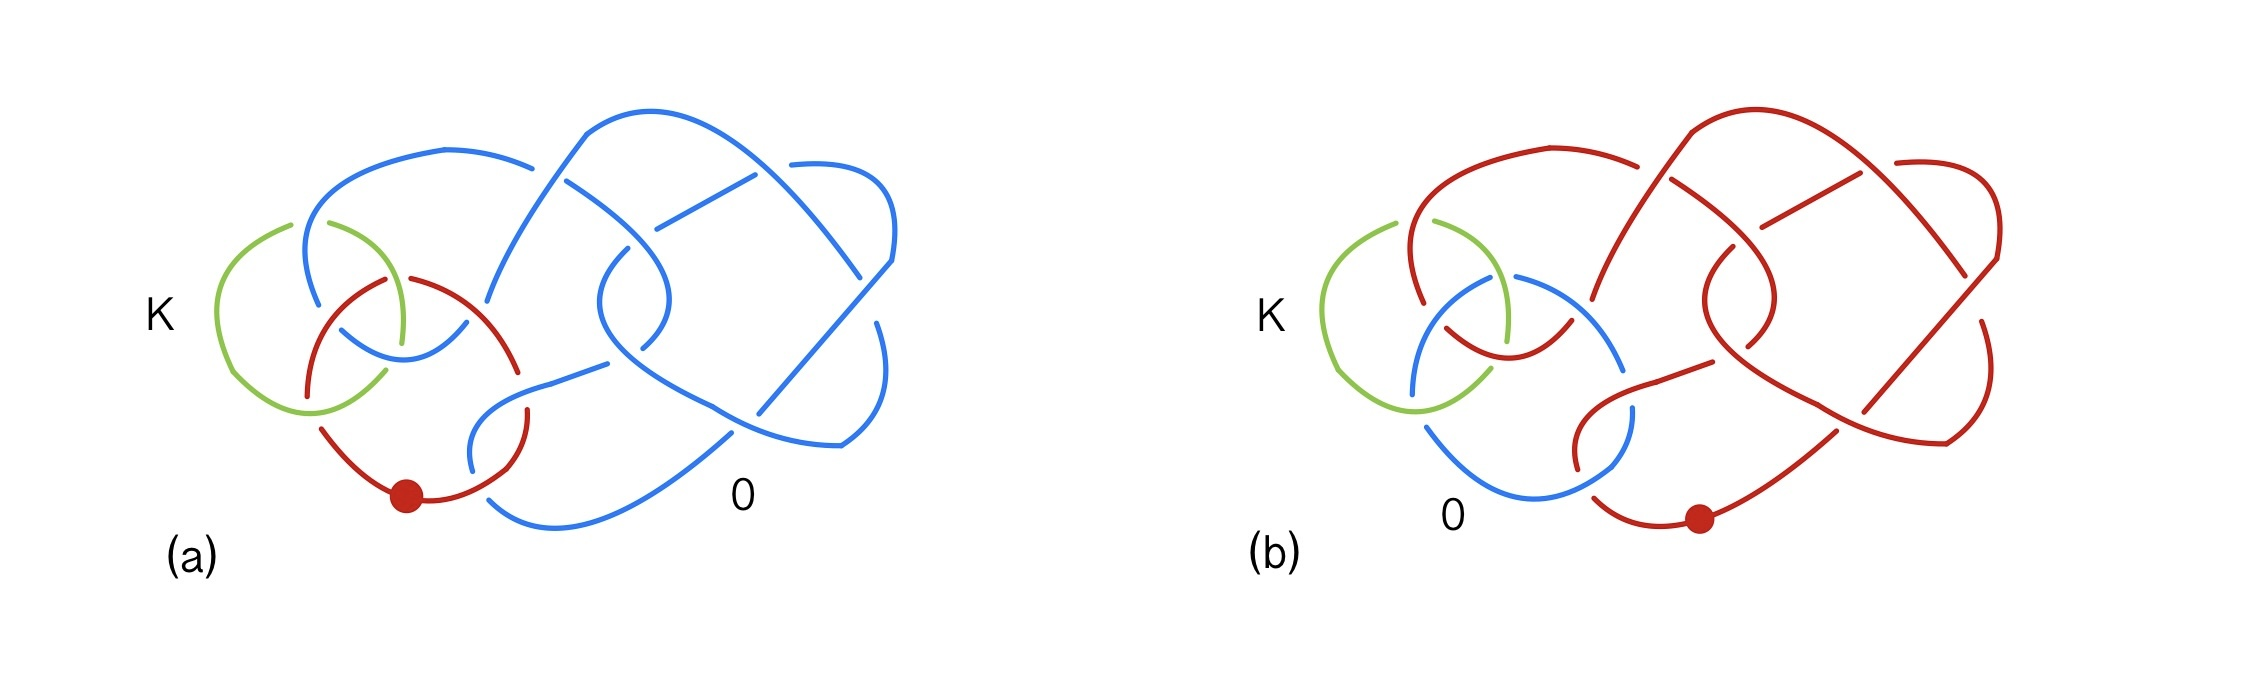
\includegraphics[scale=0.2]{figures/trecolori.jpeg}
    \caption{Two Kirby diagrams decorated with colors to enhance the roles of the handles}
    \label{fig:trecolori}
\end{figure}
\begin{obs}$\mathfrak{K}$ represents $\B^4$. 
\end{obs}
In fact, after a small isotopy, the core of the $1$-handle transversely intersects the cocore of the $2$ handle in one point. Therefore, we can perform a handle cancellation, that turns $D$ into the empty diagram. \\ \\
Let the third component of the quasi Brunnian link be $K$.
With this interpretation in mind, $K$ is a knot sitting inside $\partial \B^4 = \s^3$, presented with a non - standard surgery diagram. 
\begin{cla}$K$ bounds a slice disk, embedded in $\B^4$.
\end{cla}
The key point is that $K$ does not pass through the $1$-handle.
Clearly $K$ bounds a disk $D$ in $\s^3 \setminus A$. We then push the interior of $D$ in the interior of $\B^4 \cup (1-handle) = \s^1 \times \B^3$.
As a result, $D$ does not interfere with the attaching region of the $2$-handle.
Notice that this is possible because $A \cup K$ is split.
This procedure gives rise to the desired disk. \\ \\
Since the definition of quasi Brunnian link is symmetric (with respect to $A$ and $B$), we can swap the roles of $A$ and $B$. We place the red dot on $B$, and decorate $A$ with the $0$ label, as in Figure \ref{fig:trecolori}(b). Then we produce another disk $D'$ that bounds $K$ as before. We have created a pair of embedded slice disks which bound the same knot. 
From what has been said so far, it is not clear that such disks are ribbon.
This will become clear in the next section.
\section{Explicit Description of the Disks via Banded Unlink Diagrams}
The approach discussed above, is quite theoretical. As we will see, one can prove exoticness of the pair, in the topological setting, without any further description of $D$ and $D'$.
However, a bare hand approach may be mandatory to prove other properties of the disks. 
We start by redrawing $K$ in the standard surgery diagram of $\s^3$. At this point, we have a few options. \\ \\ In general, we can use the following algoritmic approach. We isotope $A \cup B$ to a Hopf link and we drag $K$ along such isotopy. Then, we perform multiple handle slides ($K$ over the $2$ handle), to unlink $K$ from the red circle. Then $K$ squishes through the blue circle. Now we can cancel the handle pair, and contemplate $K$ in the empty diagram of $\partial \B^4$. \\ \\
In some lucky cases, we can perform handle slides right away. It is the case of Figure \ref{fig:mag1}(a). After a small isotopy, we can immediately perform handle slides as in Figure \ref{fig:mag1}(c), (e). From (f) to (g) we use the light bulb trick to unlink $K$ from the $2$-handle, and then we cancel the handle pair (in the boundary). Figure \ref{fig:mag2}(h) depicts $K$ in the standard diagram of $\s^3$.
\begin{note} 
The boxed integer indicates a certain number of negative full twists. We will also allow half integers, meaning half twists. 
\begin{obs} \label{unico}
Since Kirby moves correspond to diffeomorphisms of $\B^4$ and since the mapping class group of $\s^3$ is trivial, every sequence of isotopies and Kirby moves leads to the same knot, up to isotopy.
\end{obs}
Roughly speaking, it is only a shift of perspective.
\end{note}
\begin{figure}[H]
    \centering
    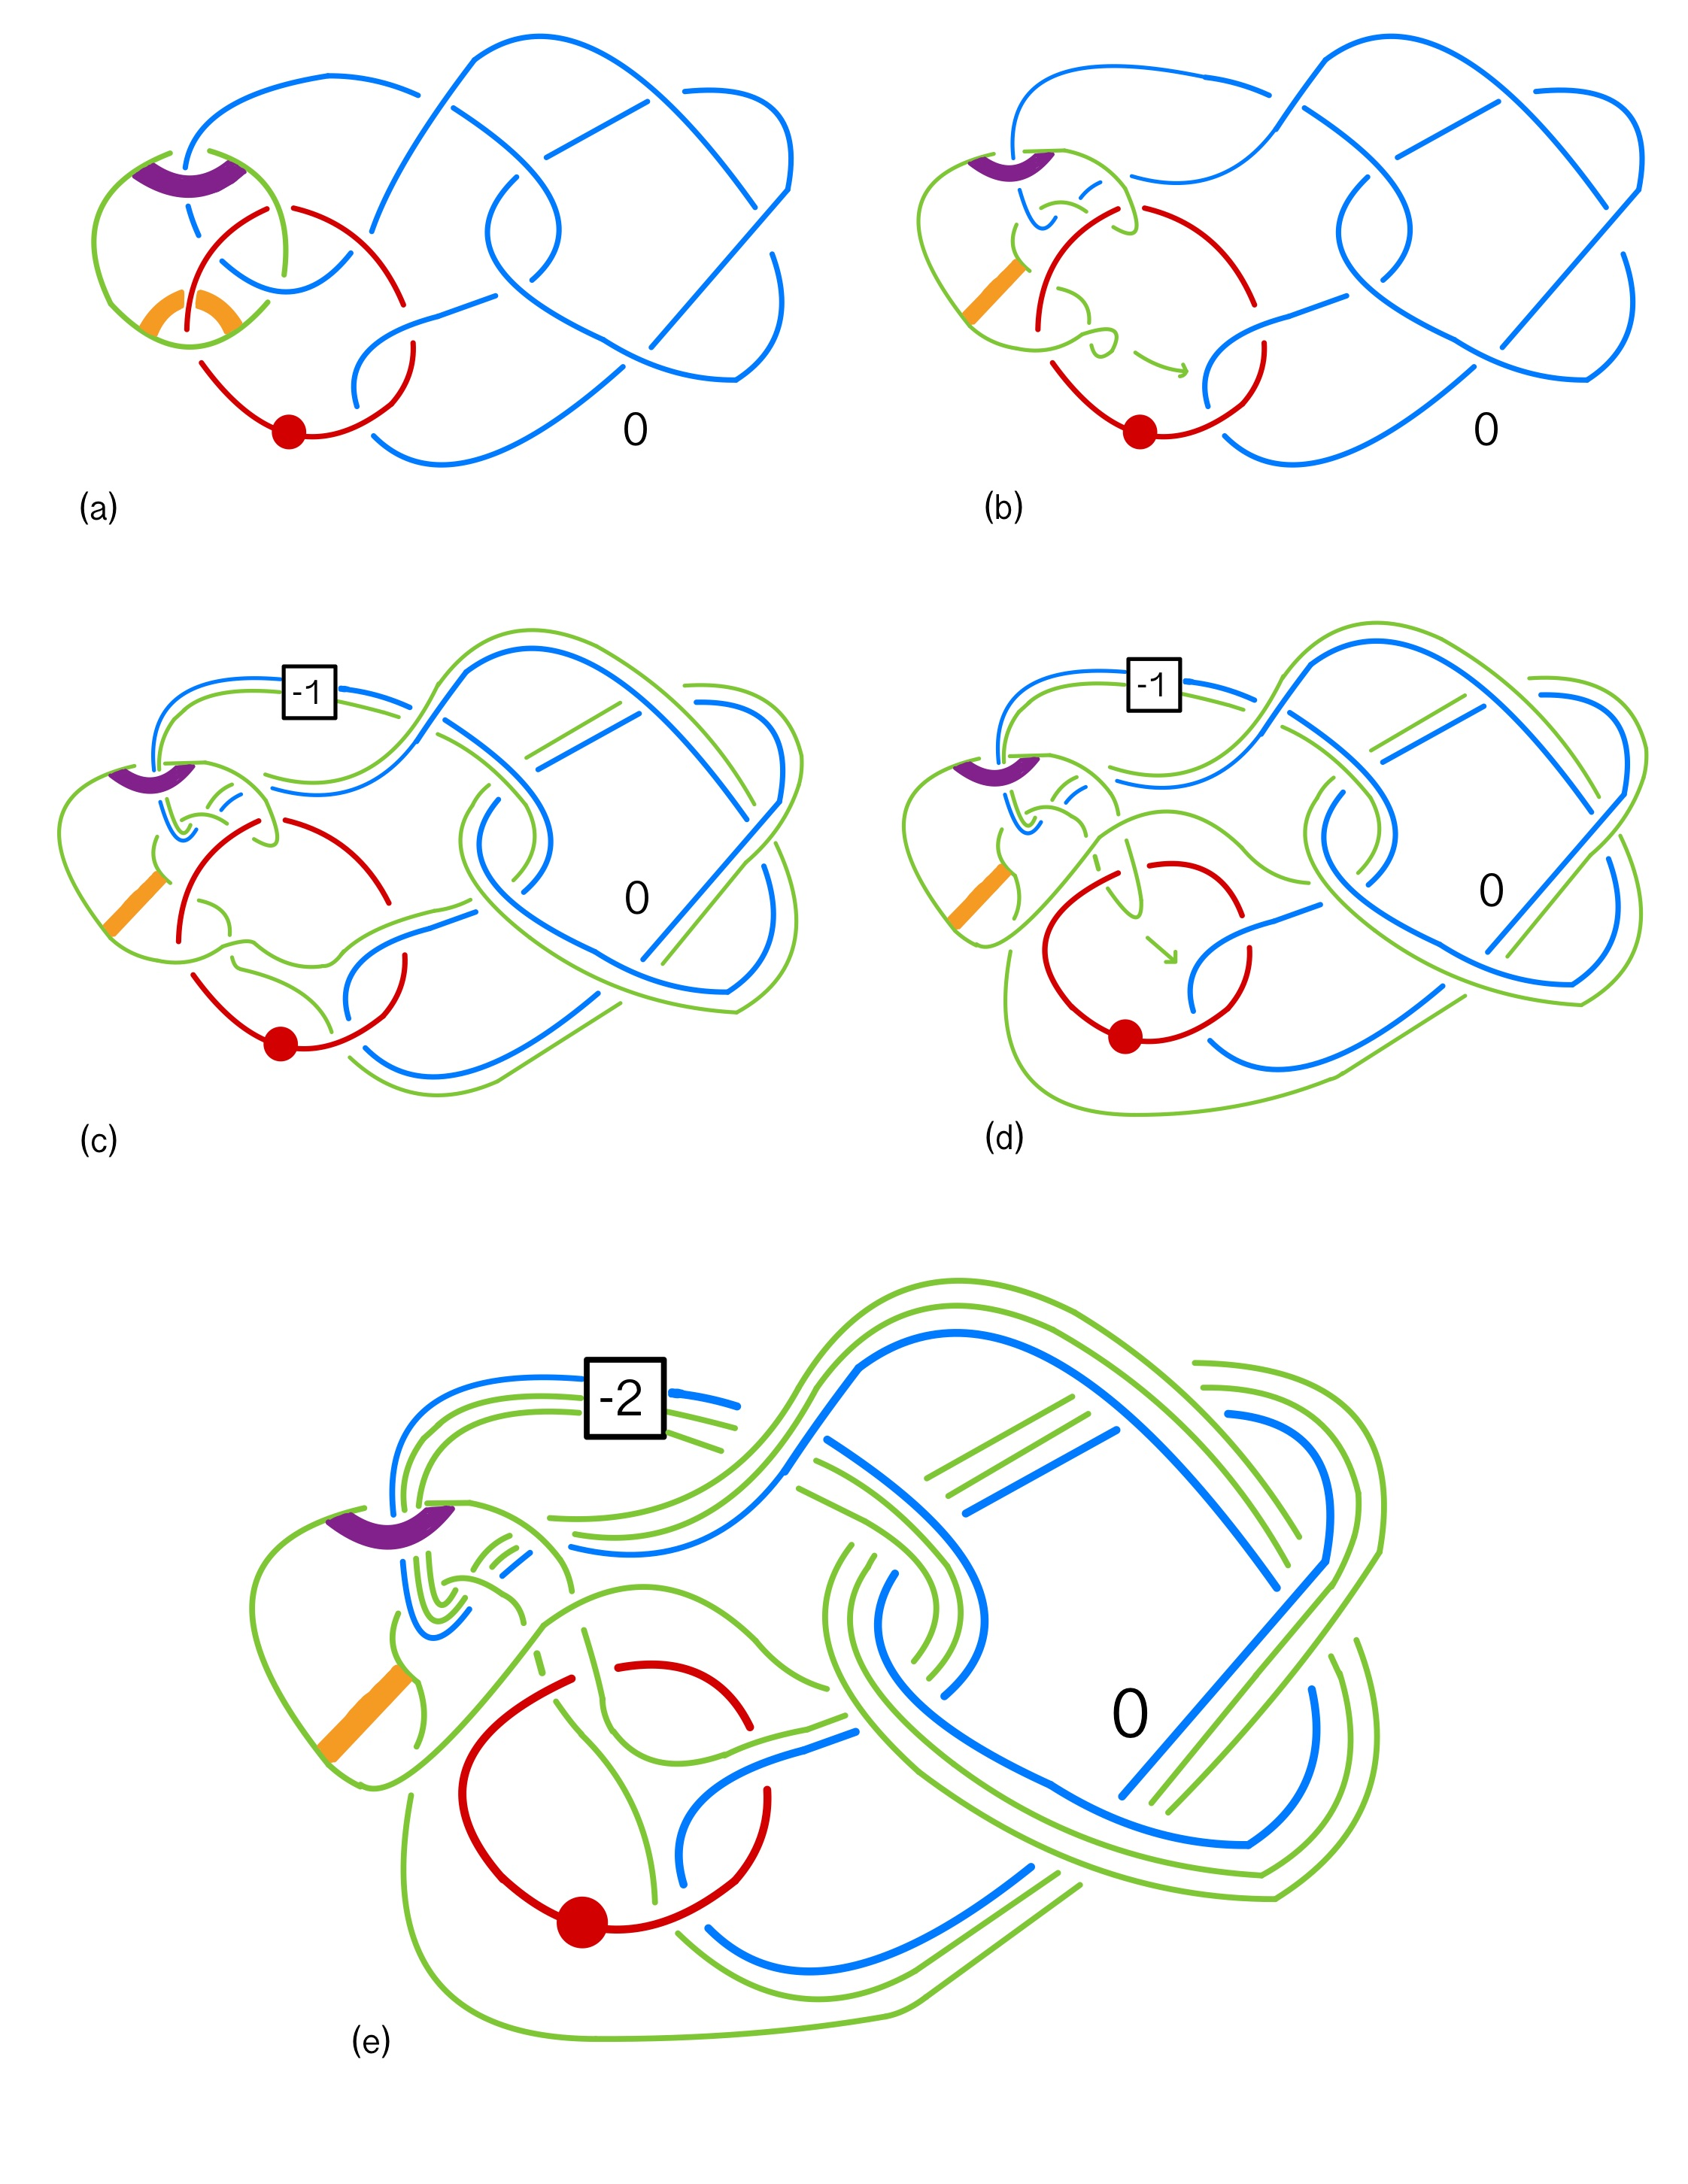
\includegraphics[scale=0.2]{figures/mag1.jpeg}
    \caption{A sequence of isotopies and Kirby moves}
    \label{fig:mag1}
\end{figure}
\begin{figure}[H]
    \centering
    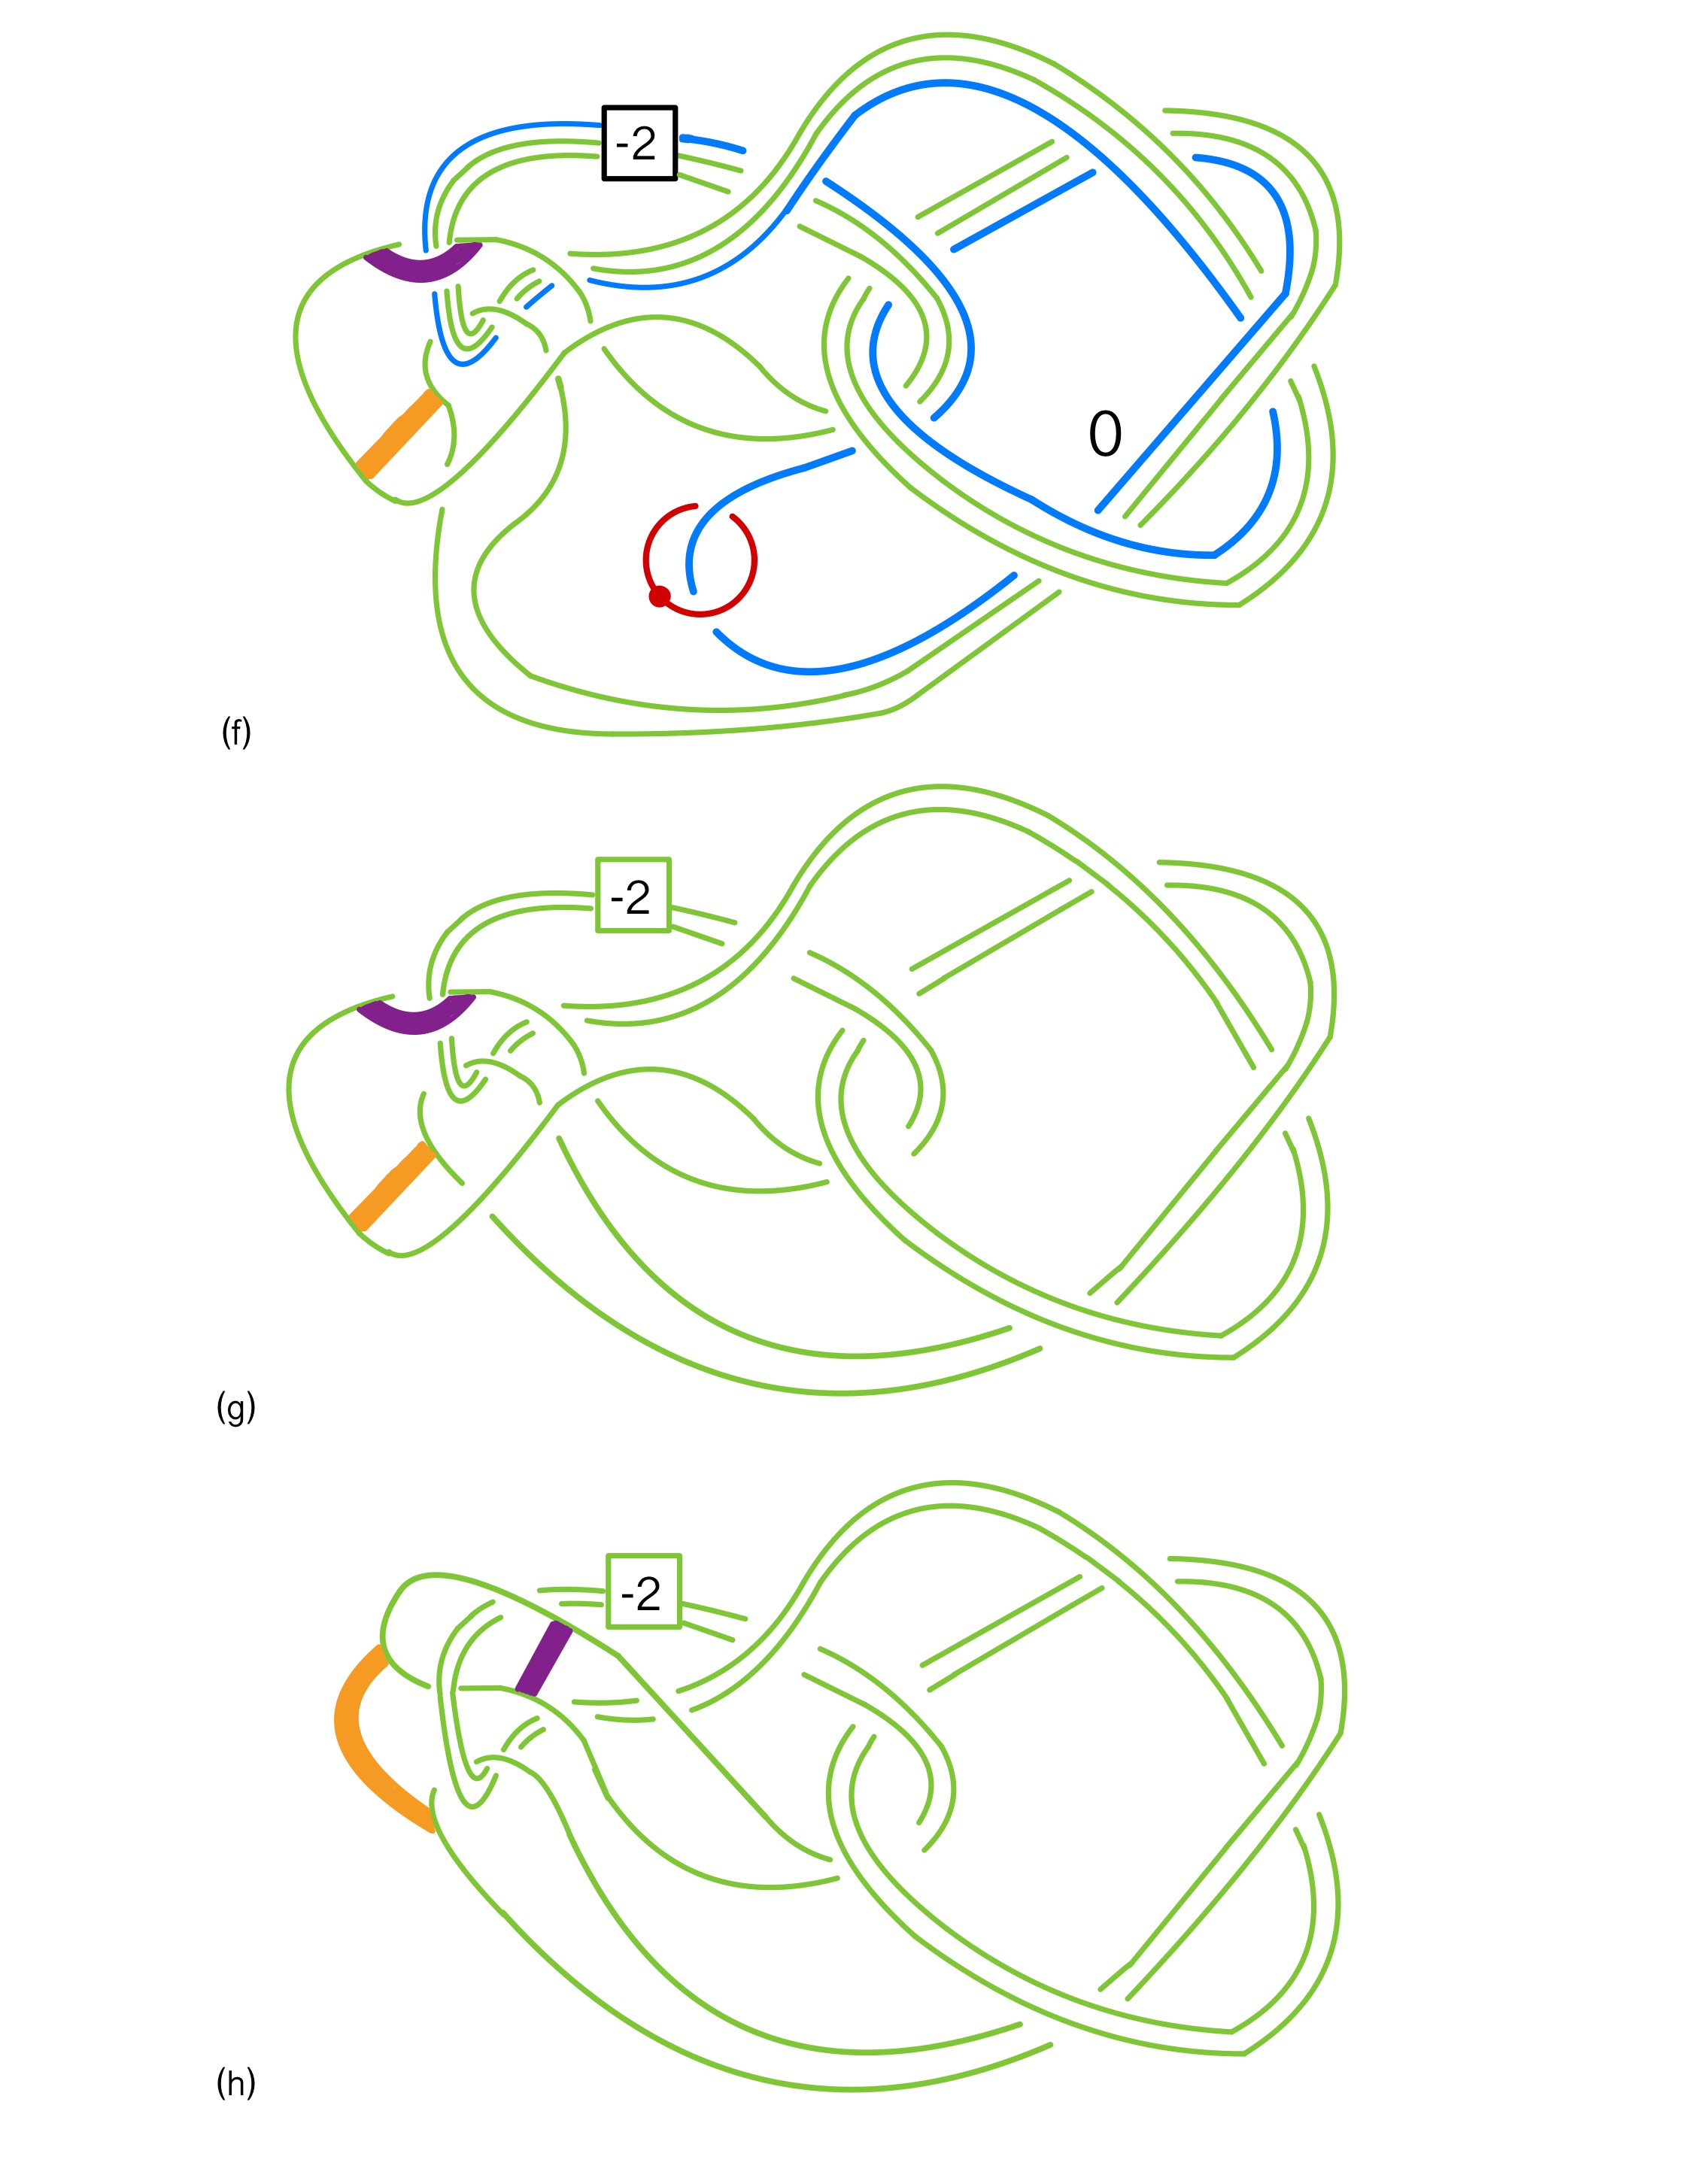
\includegraphics[scale=0.2]{figures/mag2.jpeg}
    \caption{A sequence of isotopies}
    \label{fig:mag2}
\end{figure}
In the previous figures, we kept track of two bands. 
\begin{as}The two bands, depicted in Figure \ref{fig:mag2}(h), define the disks $D$, $D'$ arising from the construction.
\end{as}
\proof
For background on banded unlink diagrams, we refer the reader to \cite{Hughes_2020}.
Consider the first picture \ref{fig:mag1}(a). 
The disk $D$ intersects the $2$-handle twice, resulting in two local minima in $\B^4$, which are cocores of the $2$-handle. The same is true for $D'$ after swapping the red with the blue circle2. Thus, there is only one ribbon band defining each disk \footnote{Each disk is almost described in the actual diagram where $K$ is a unknot}. Observe that band surgery on the orange band turns $K$ into two meridians for the red circle. On the other hand, band surgery on the purple band turns $K$ into two meridians for the blue circle. Thus, we identify the desired bands.
\endproof
It is now clear that $D$ and $D'$ are ribbon disks. \\
If we think about these bands, we can realize that they are pretty obvious.
Indeed, the purple band gives the natural ribbon structure, known as the "pair of glasses". On the other hand, the orange band joins the two minima disks of the previous structure. \\ \\
The latter example highlights the construction. Now we start proving the main theorem of this chapter. We repeat the same procedure to the following diagram.
\begin{figure}[H] 
    \centering 
    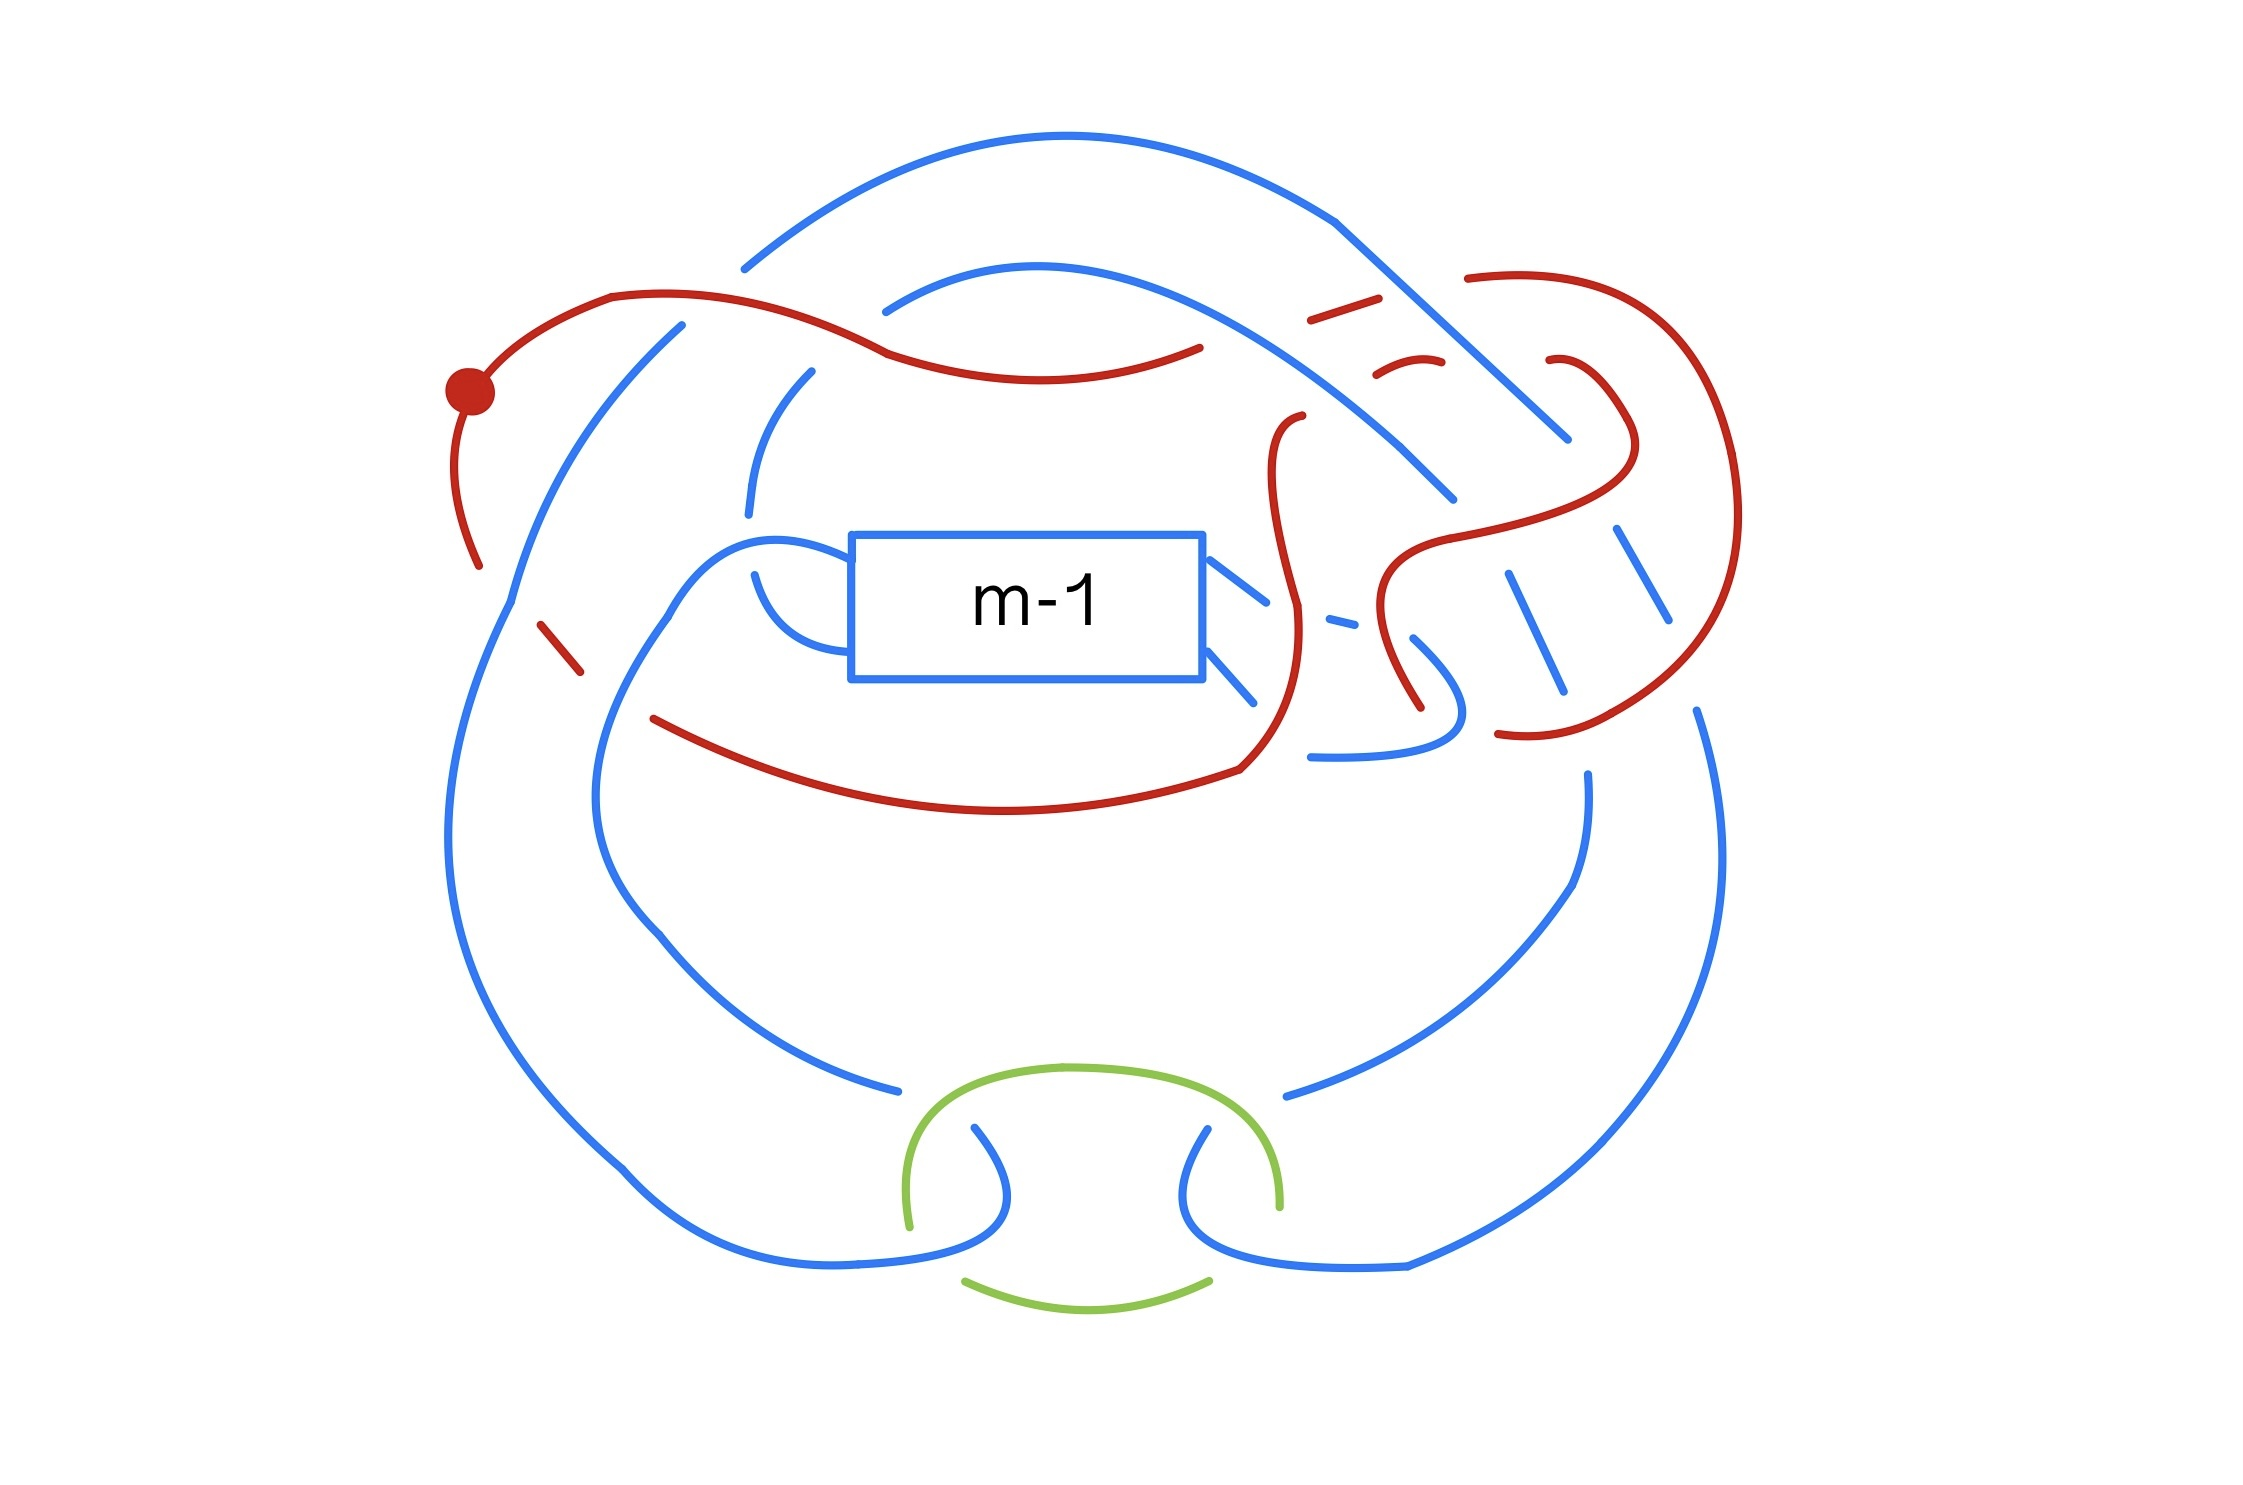
\includegraphics[scale=0.15]{figures/start.jpeg} 
    \caption{Another example of a quasi Brunnian link, labeled with colors} 
    \label{fig:start} 
\end{figure}
We call the green knot $K_m$.
We want to draw $K_m$ in the standard surgery diagram of $\s^3$. Moreover, we aim to find banded unlink diagrams of the disks $D$, $D'$ generated by Hayden's machine.
In this case we use the algoritmic approach: we turn the cancelling pair into a Hopf link. A sequence of isotopies is illustrated from Figure \ref{fig:triv1}(a) to Figure \ref{fig:triv4}(p).
\begin{figure}[H] 
    \centering 
    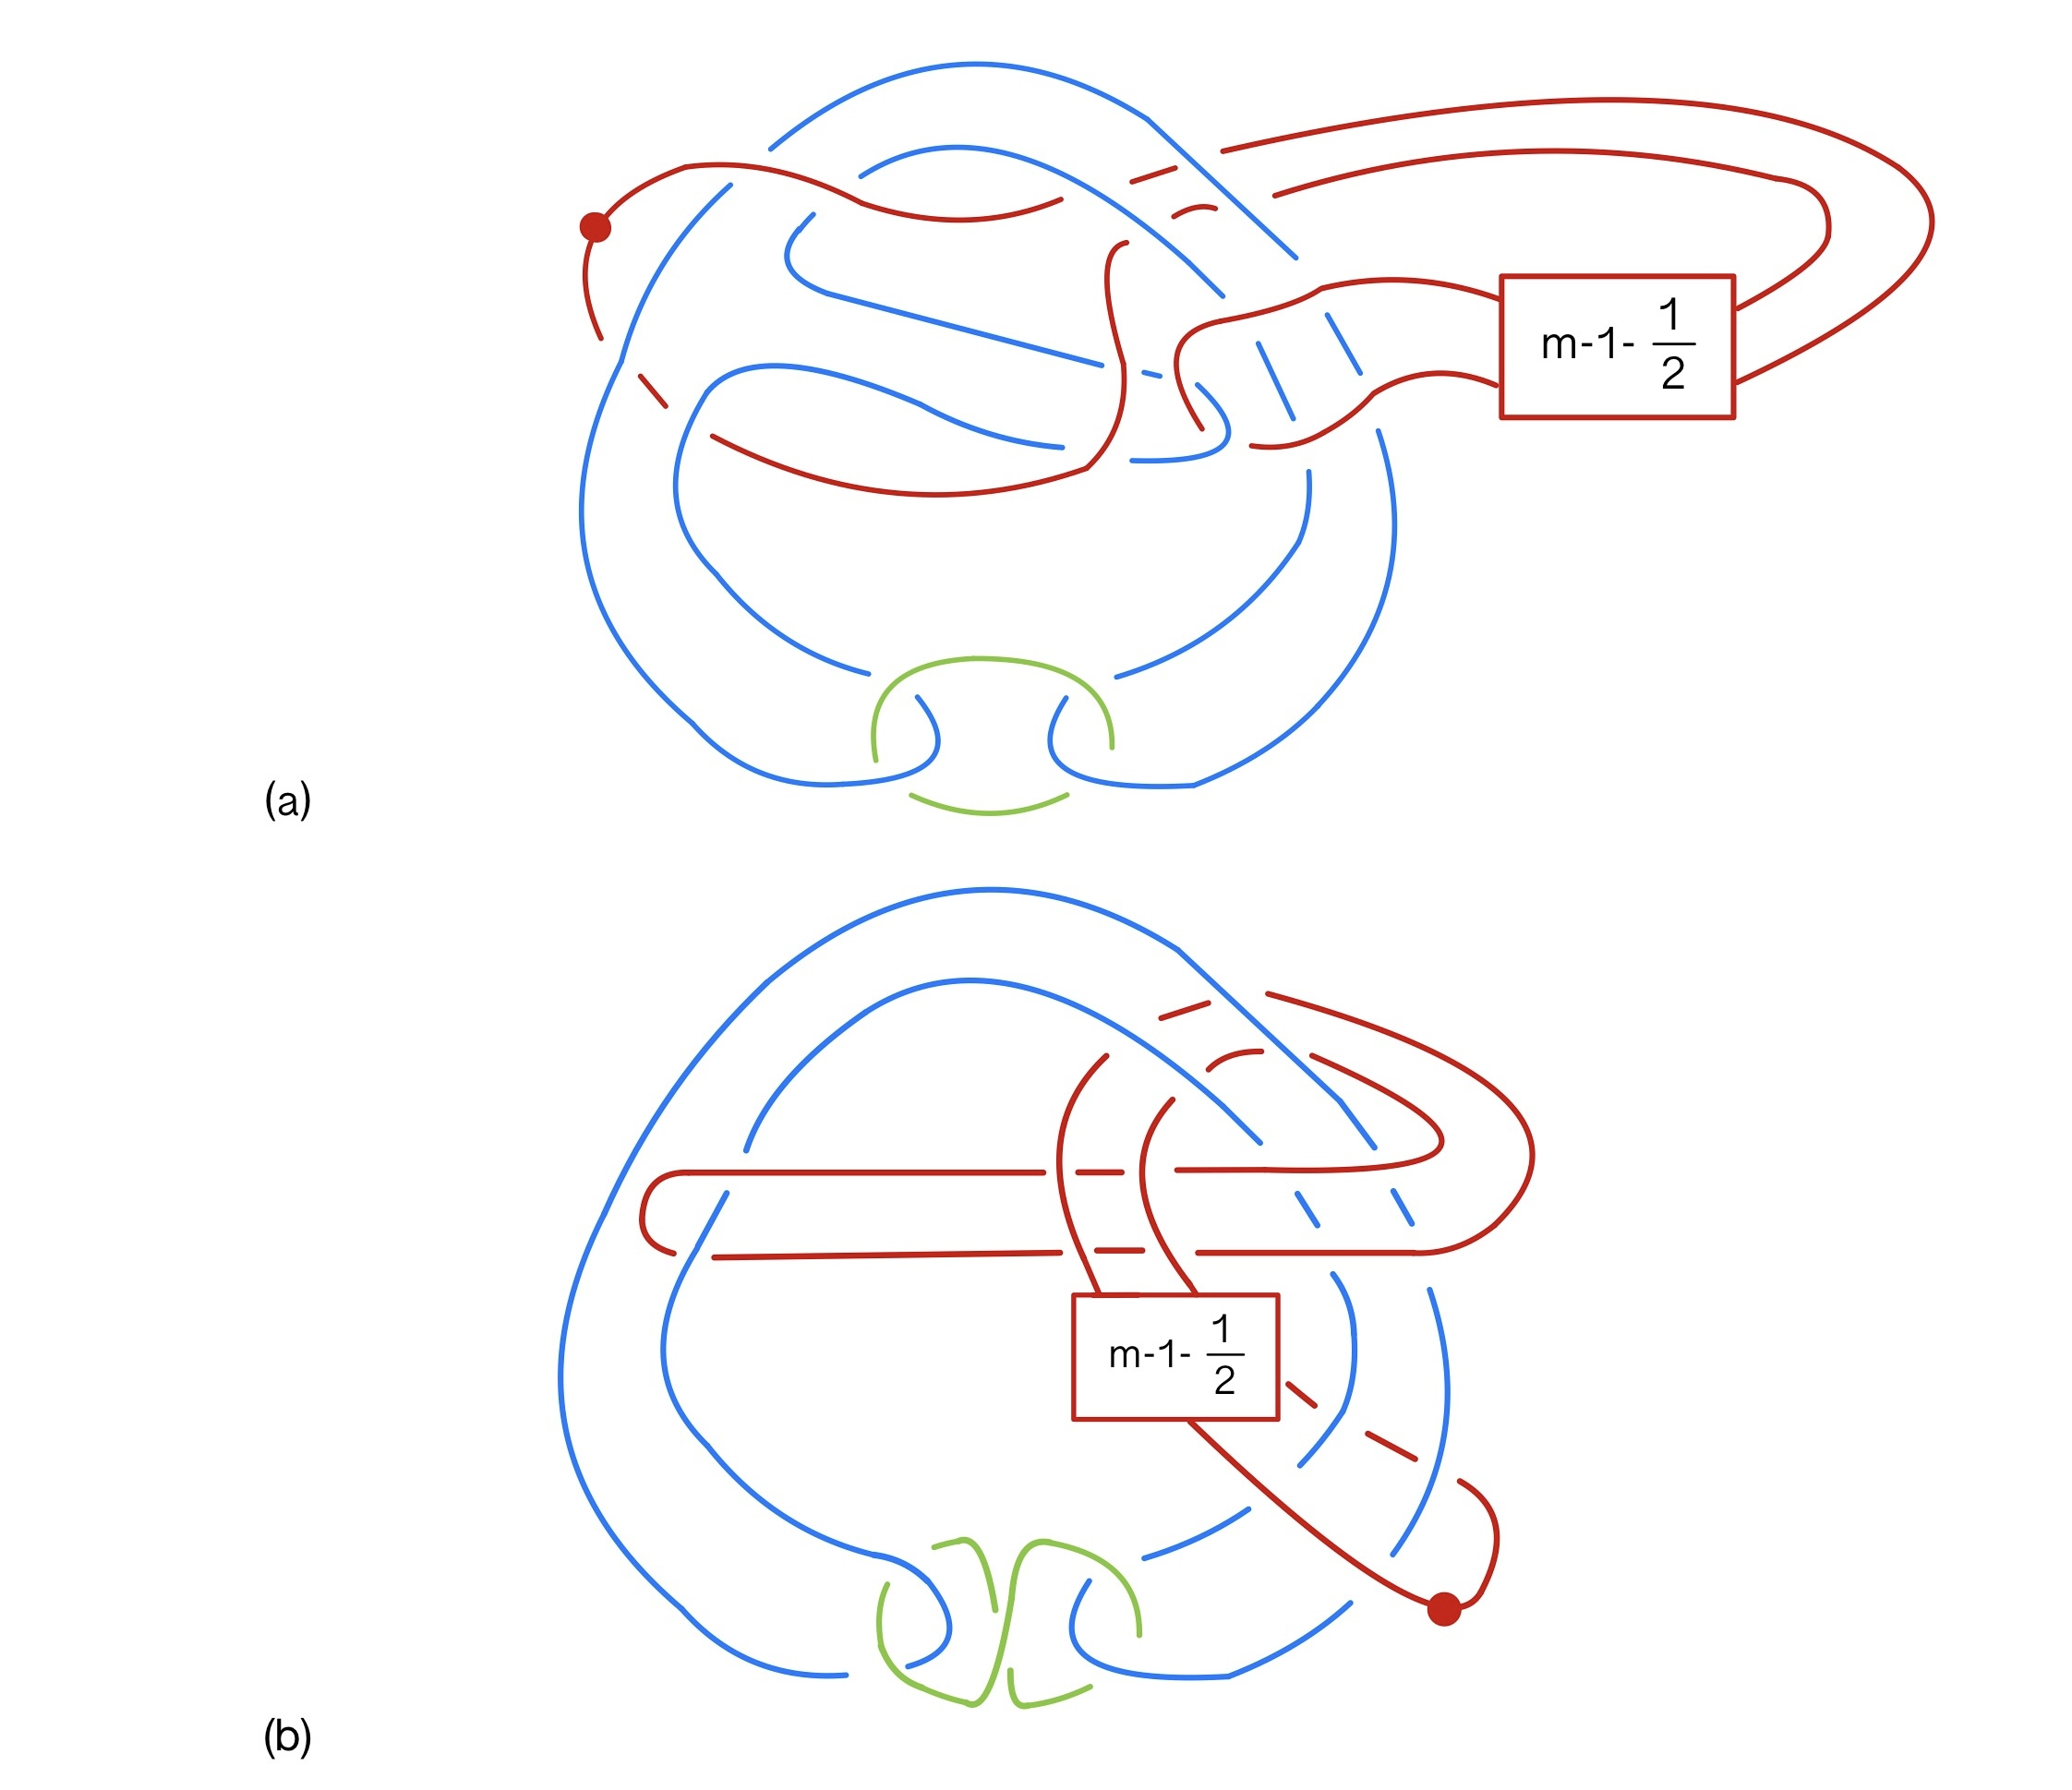
\includegraphics[scale=0.2]{figures/triv1.jpeg} 
    \caption{A sequence of isotopies} 
    \label{fig:triv1} 
\end{figure}
\begin{figure}[H] 
    \centering 
    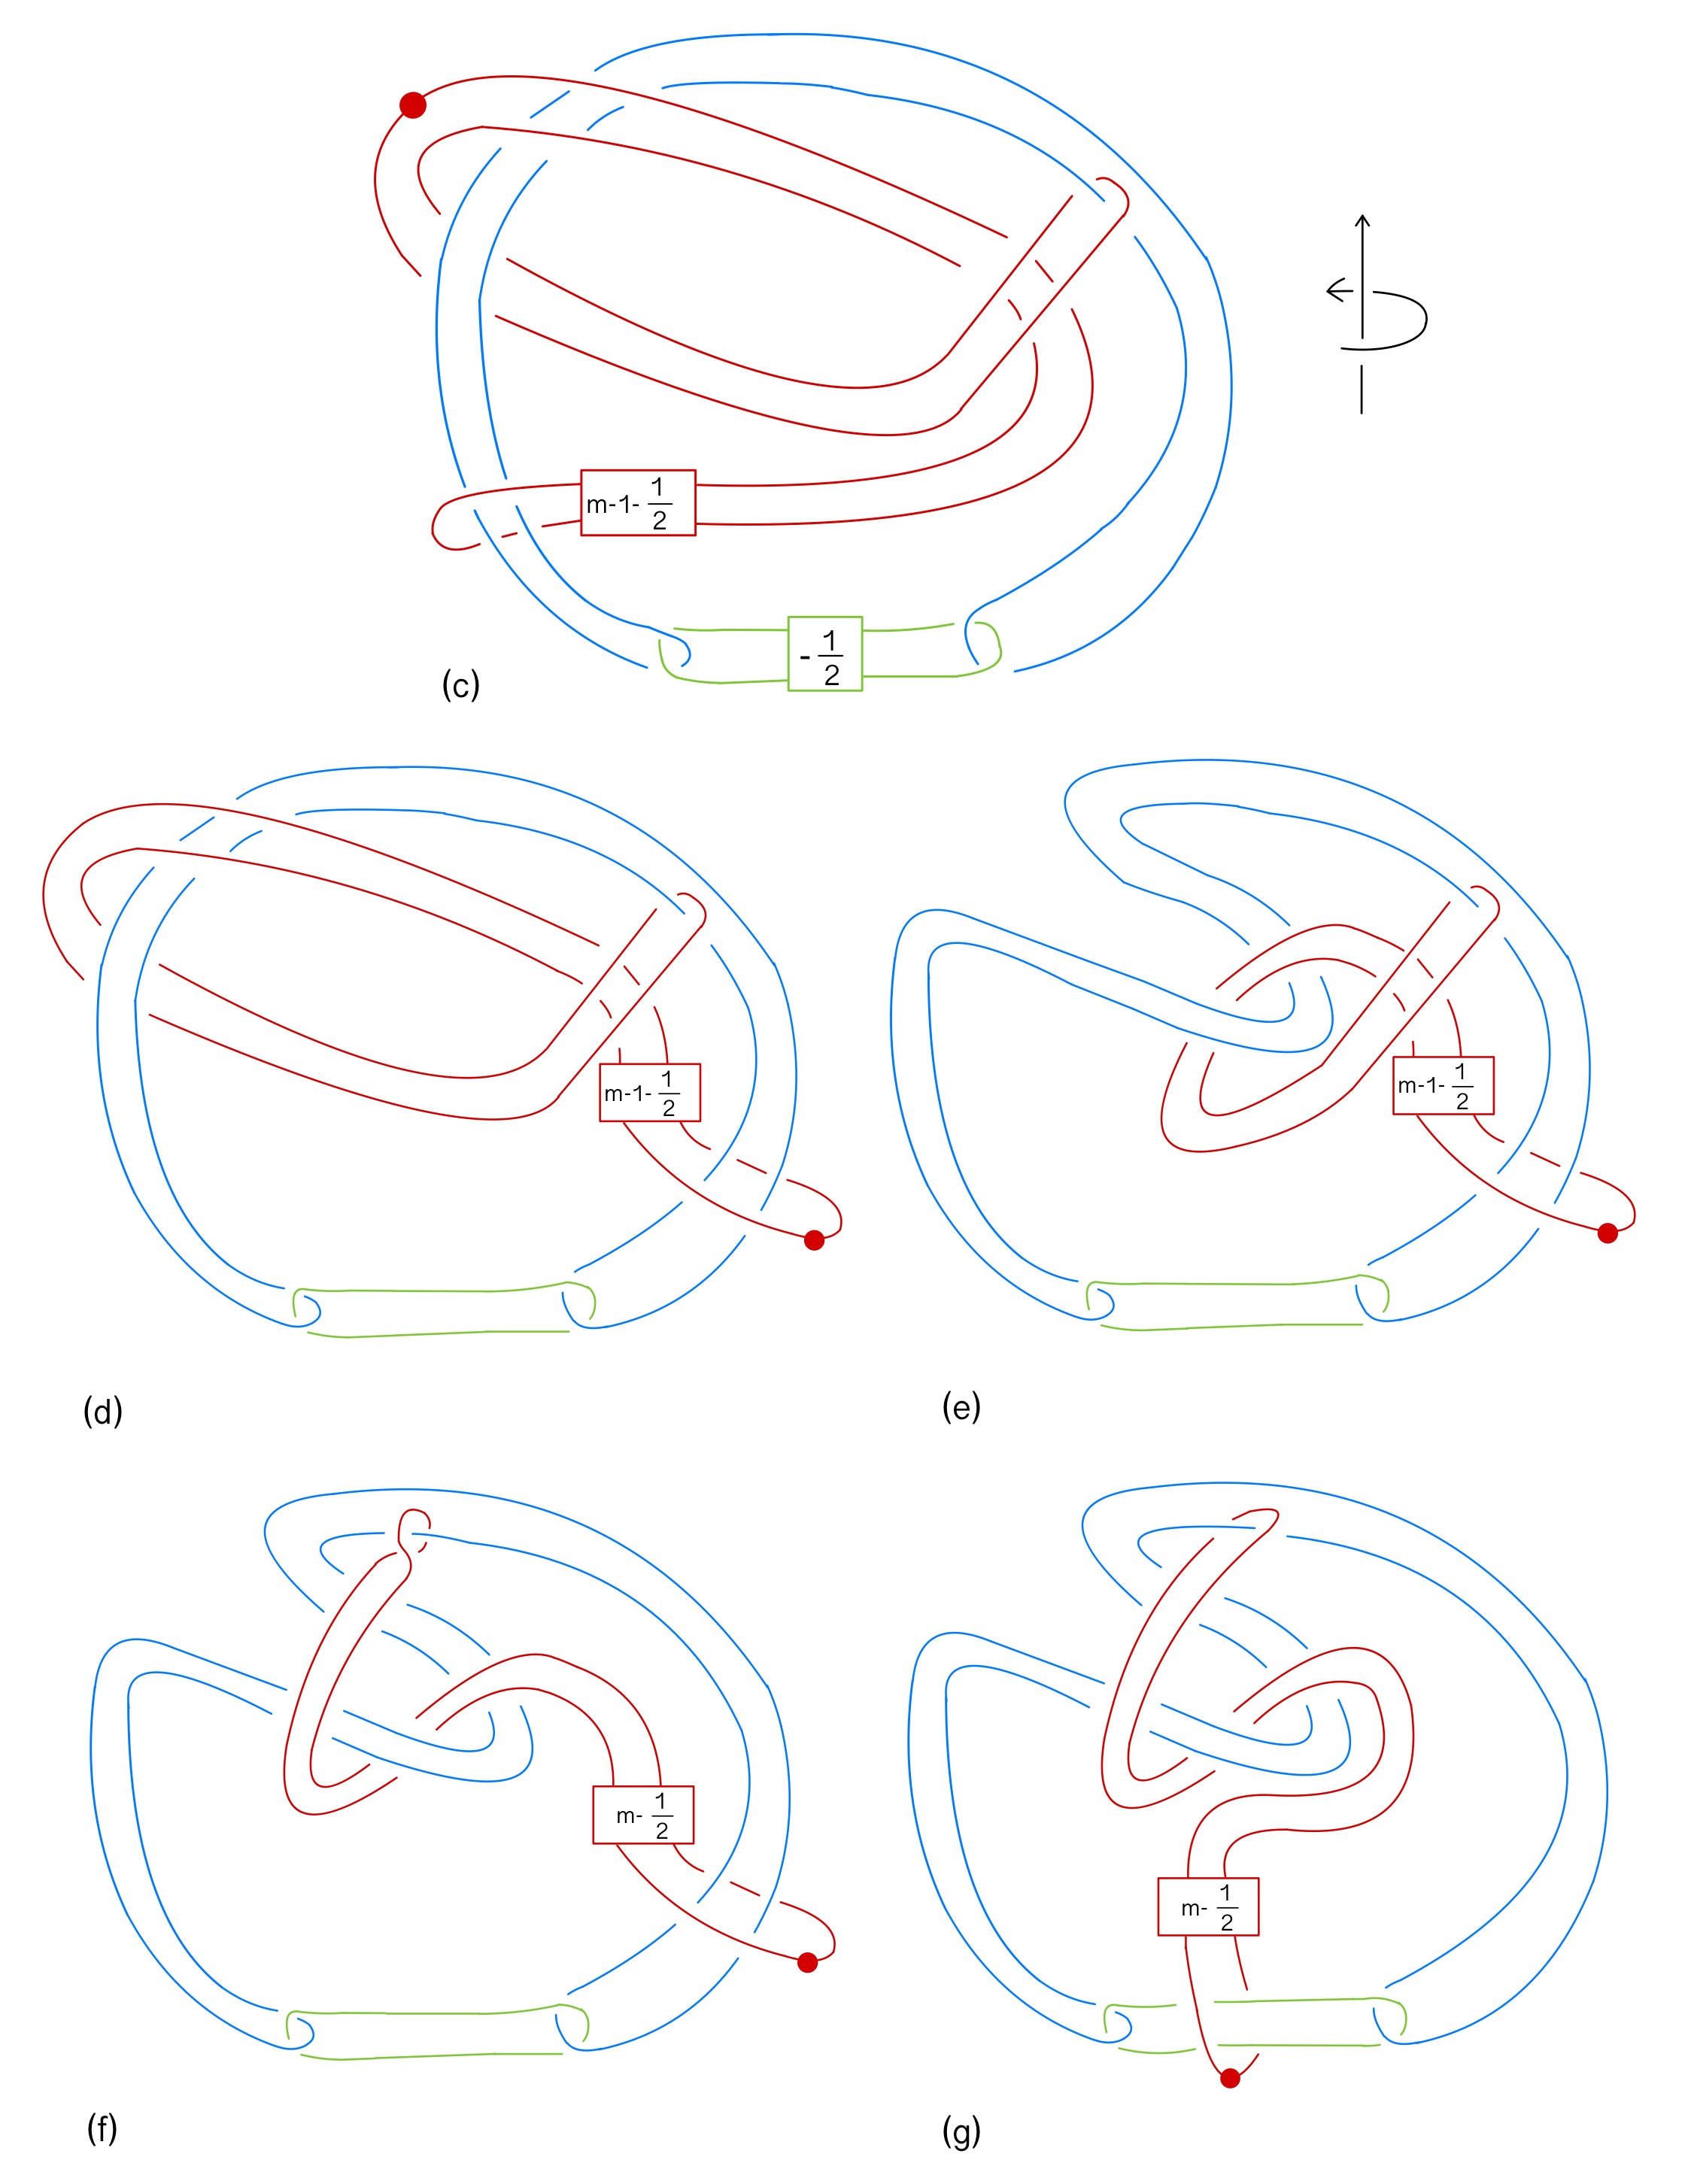
\includegraphics[scale=0.2]{figures/triv2.jpeg} 
    \caption{A sequence of isotopies} 
    \label{fig:triv2} 
\end{figure}
\begin{figure}[H] 
    \centering 
    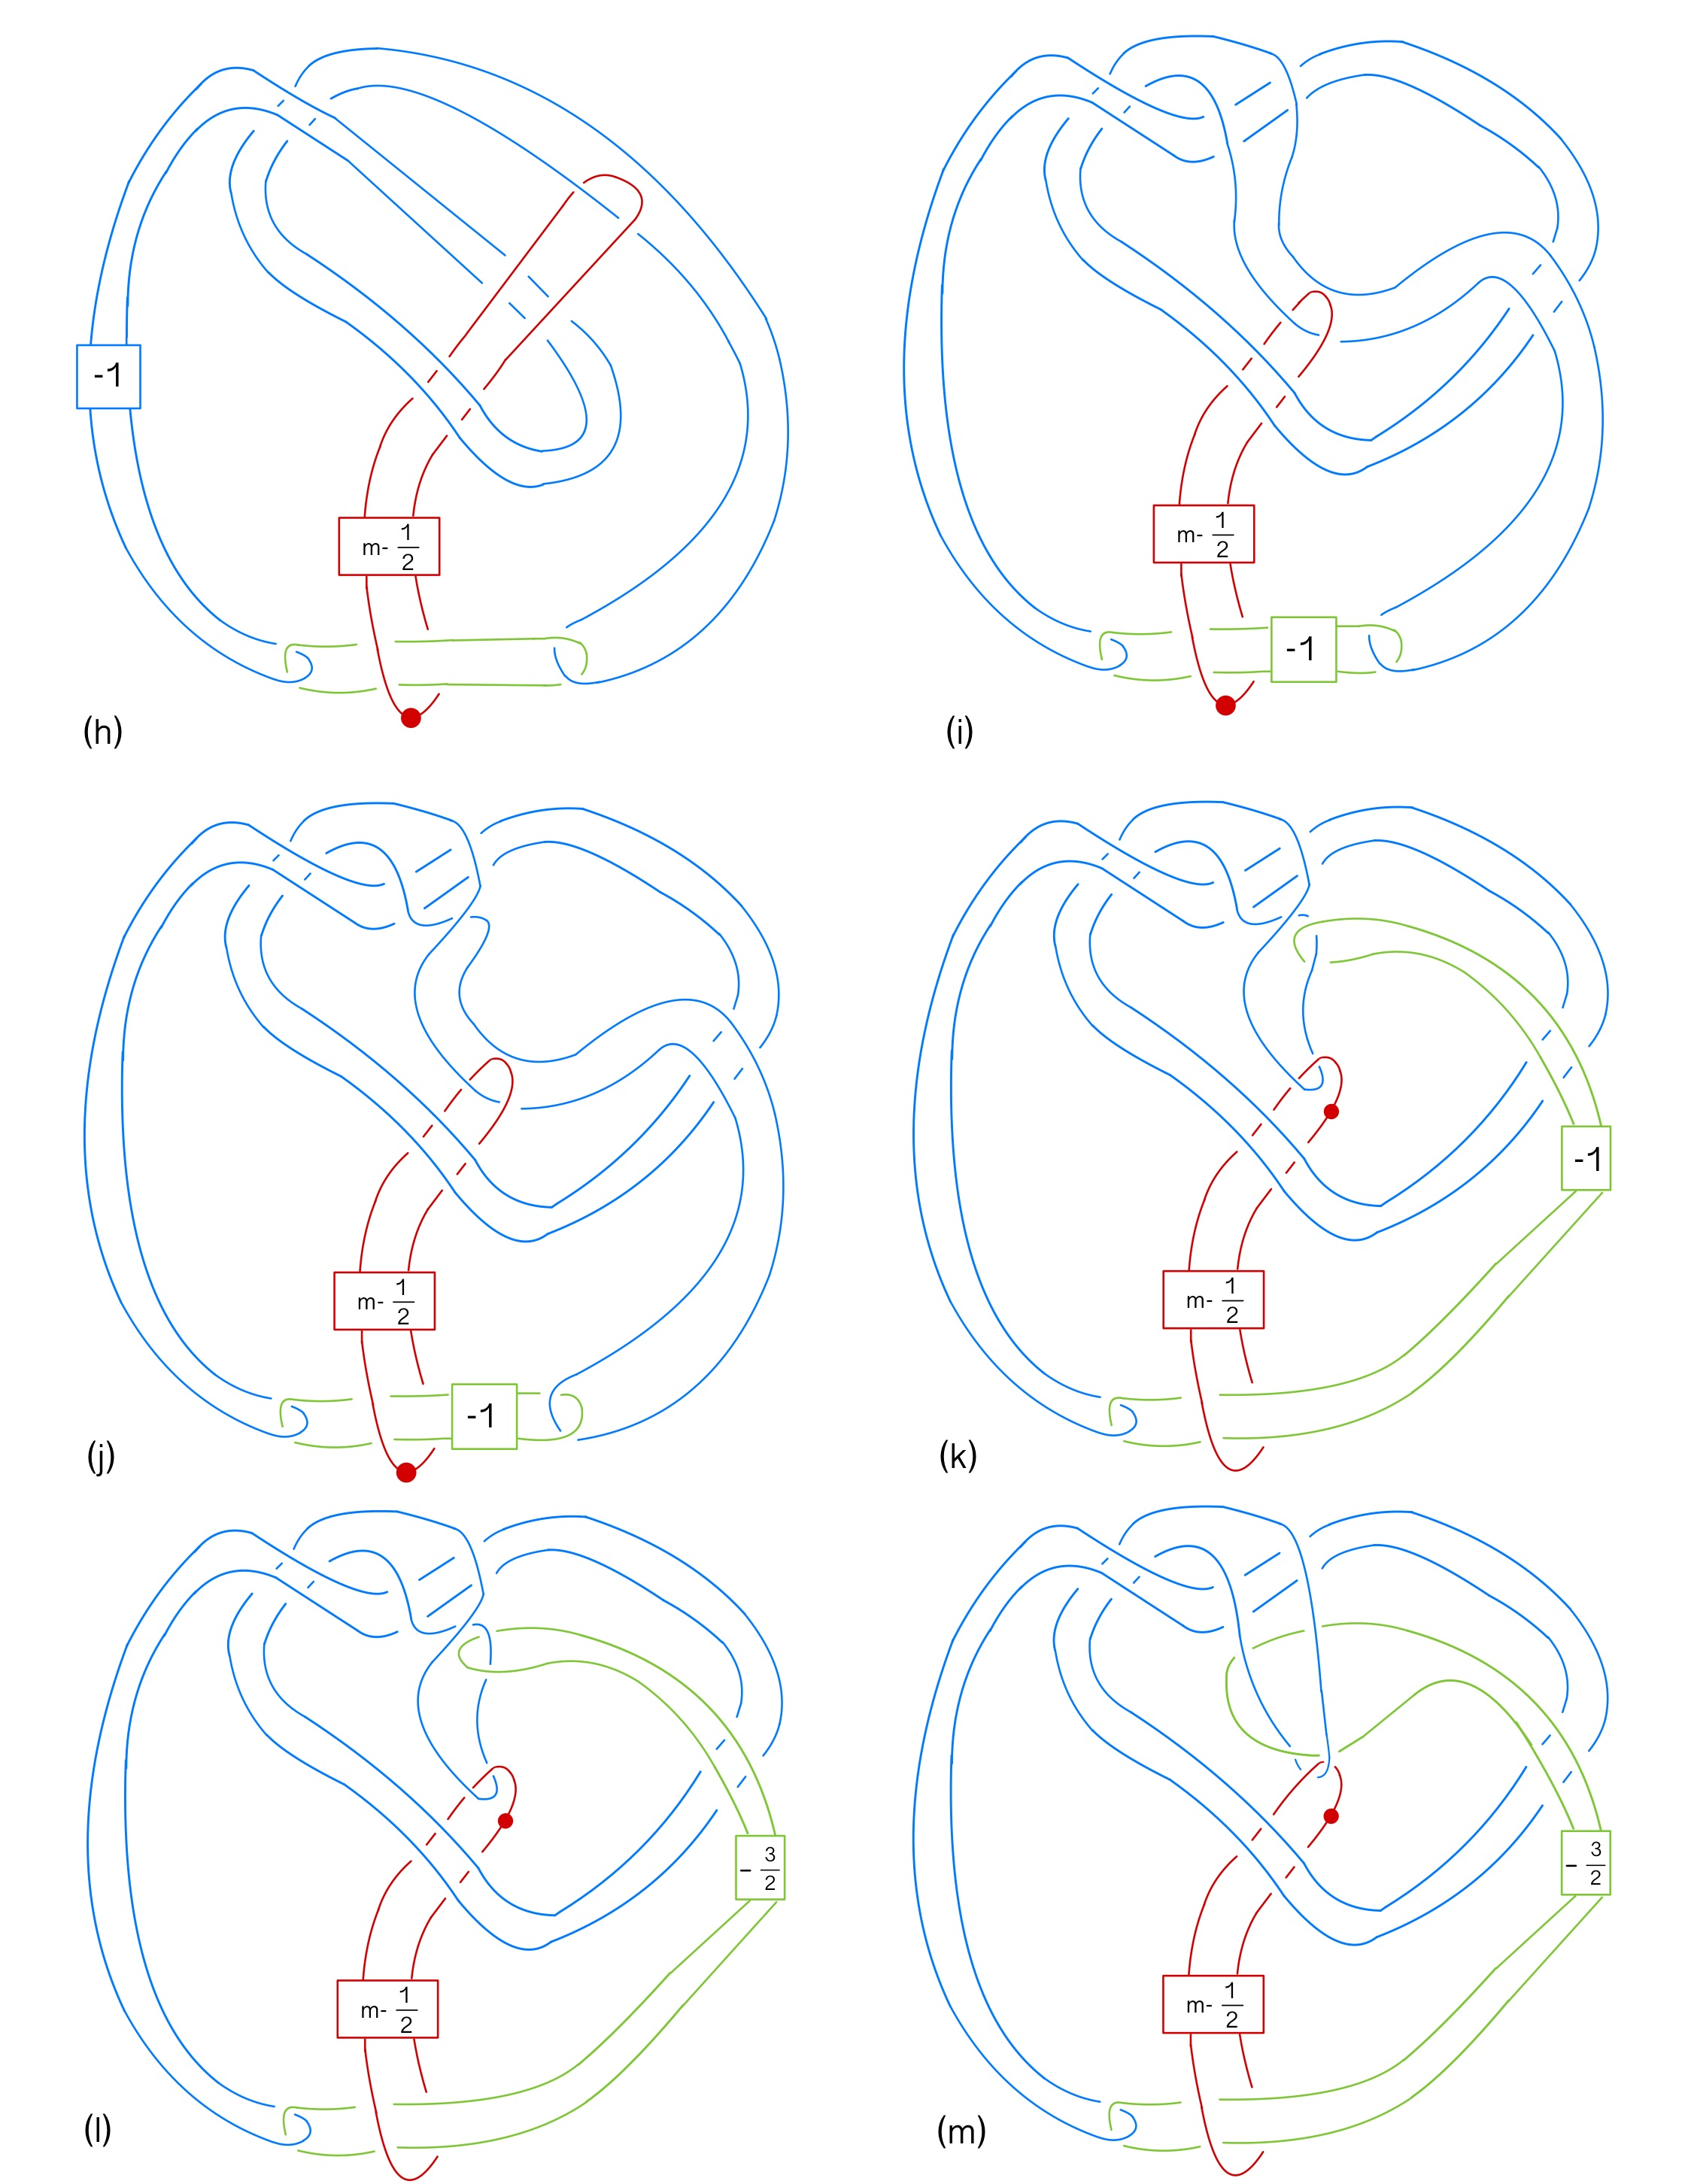
\includegraphics[scale=0.2]{figures/triv3.jpeg} 
    \caption{A sequence of isotopies} 
    \label{fig:triv3} 
\end{figure}
\begin{figure}[H] 
    \centering 
    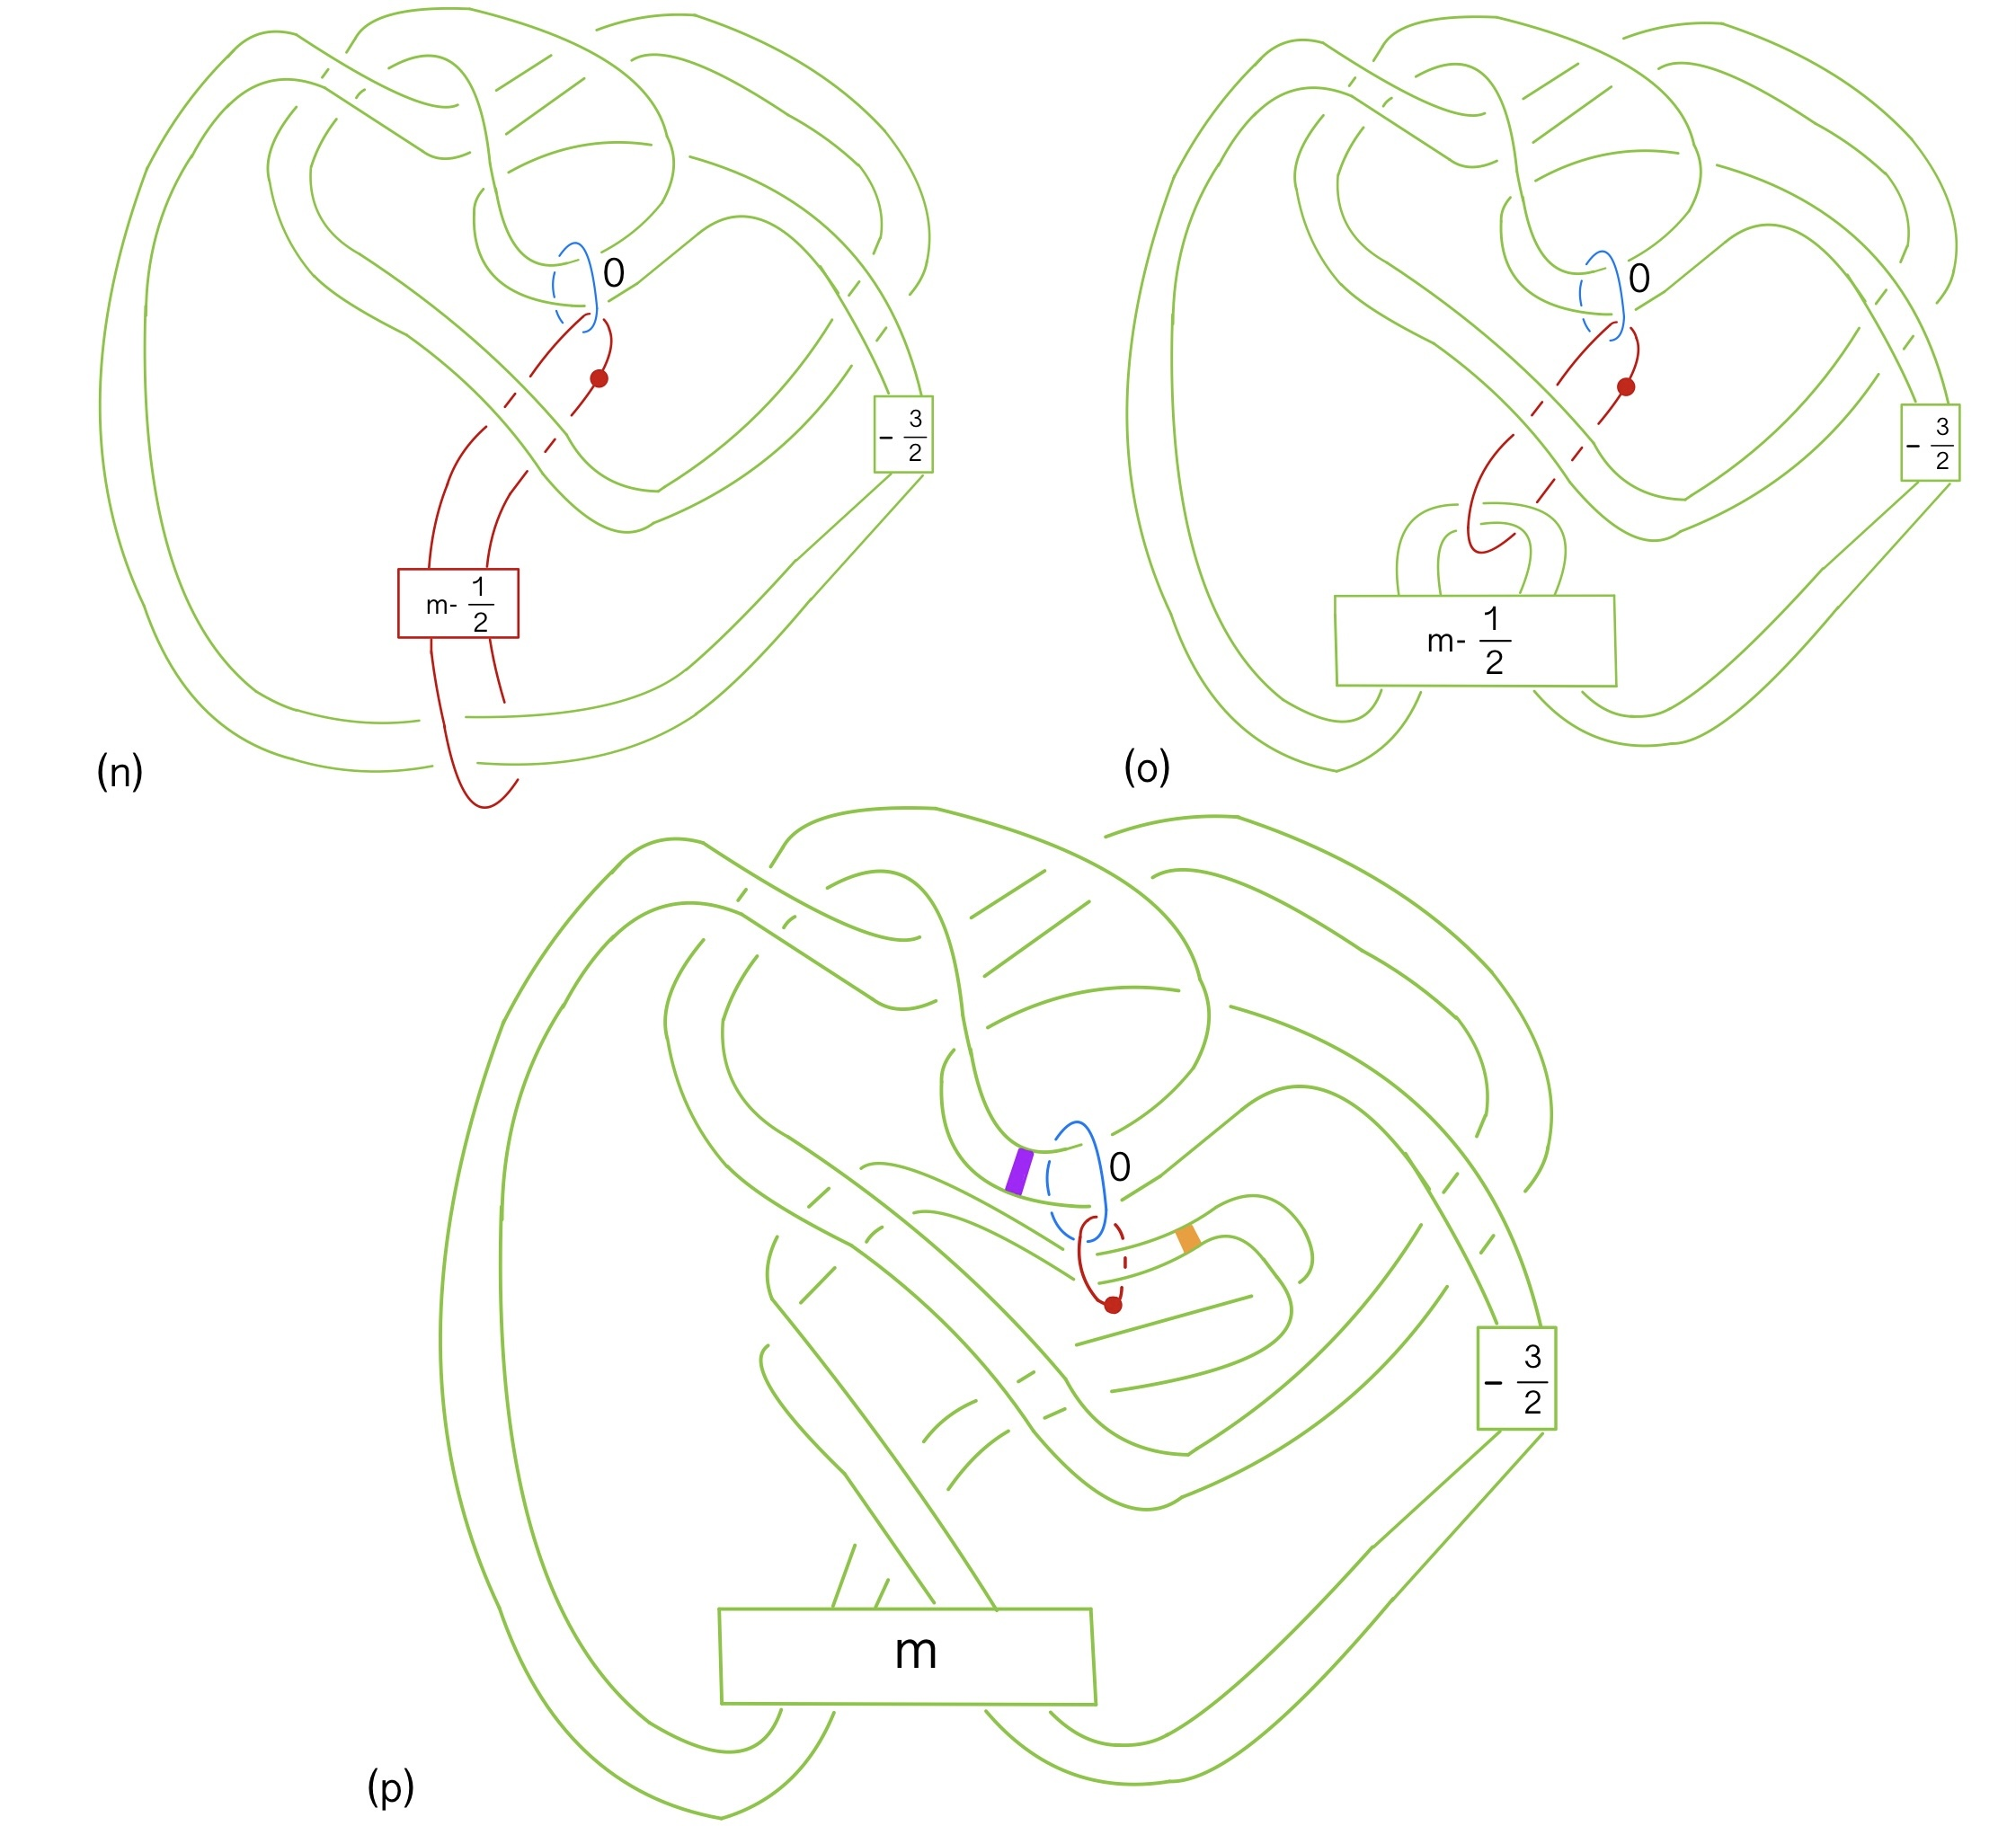
\includegraphics[scale=0.2]{figures/triv4.jpeg} 
    \caption{A sequence of isotopies} 
    \label{fig:triv4} 
\end{figure}
From now on, we track the two bands depicted in Figure \ref{fig:triv4}(p).
As in the first example, $D$ and $D'$ both have one saddle and two minima.
Notice that orange band surgery turns $K_m$ into two meridians for the blue circle. On the other hand, purple band surgery turns $K_m$ into two meridians for the red circle \ref{app} (that will be the $2$-handle after the exchange). \\
In Figure \ref{fig:triv5}(a)-(d), we slide $K_m$ two times over the $2$ handle. We include only some fragments for clarity. Figure \ref{fig:triv5}(e) shows the whole picture after the slides.
\begin{figure}[H] 
    \centering 
    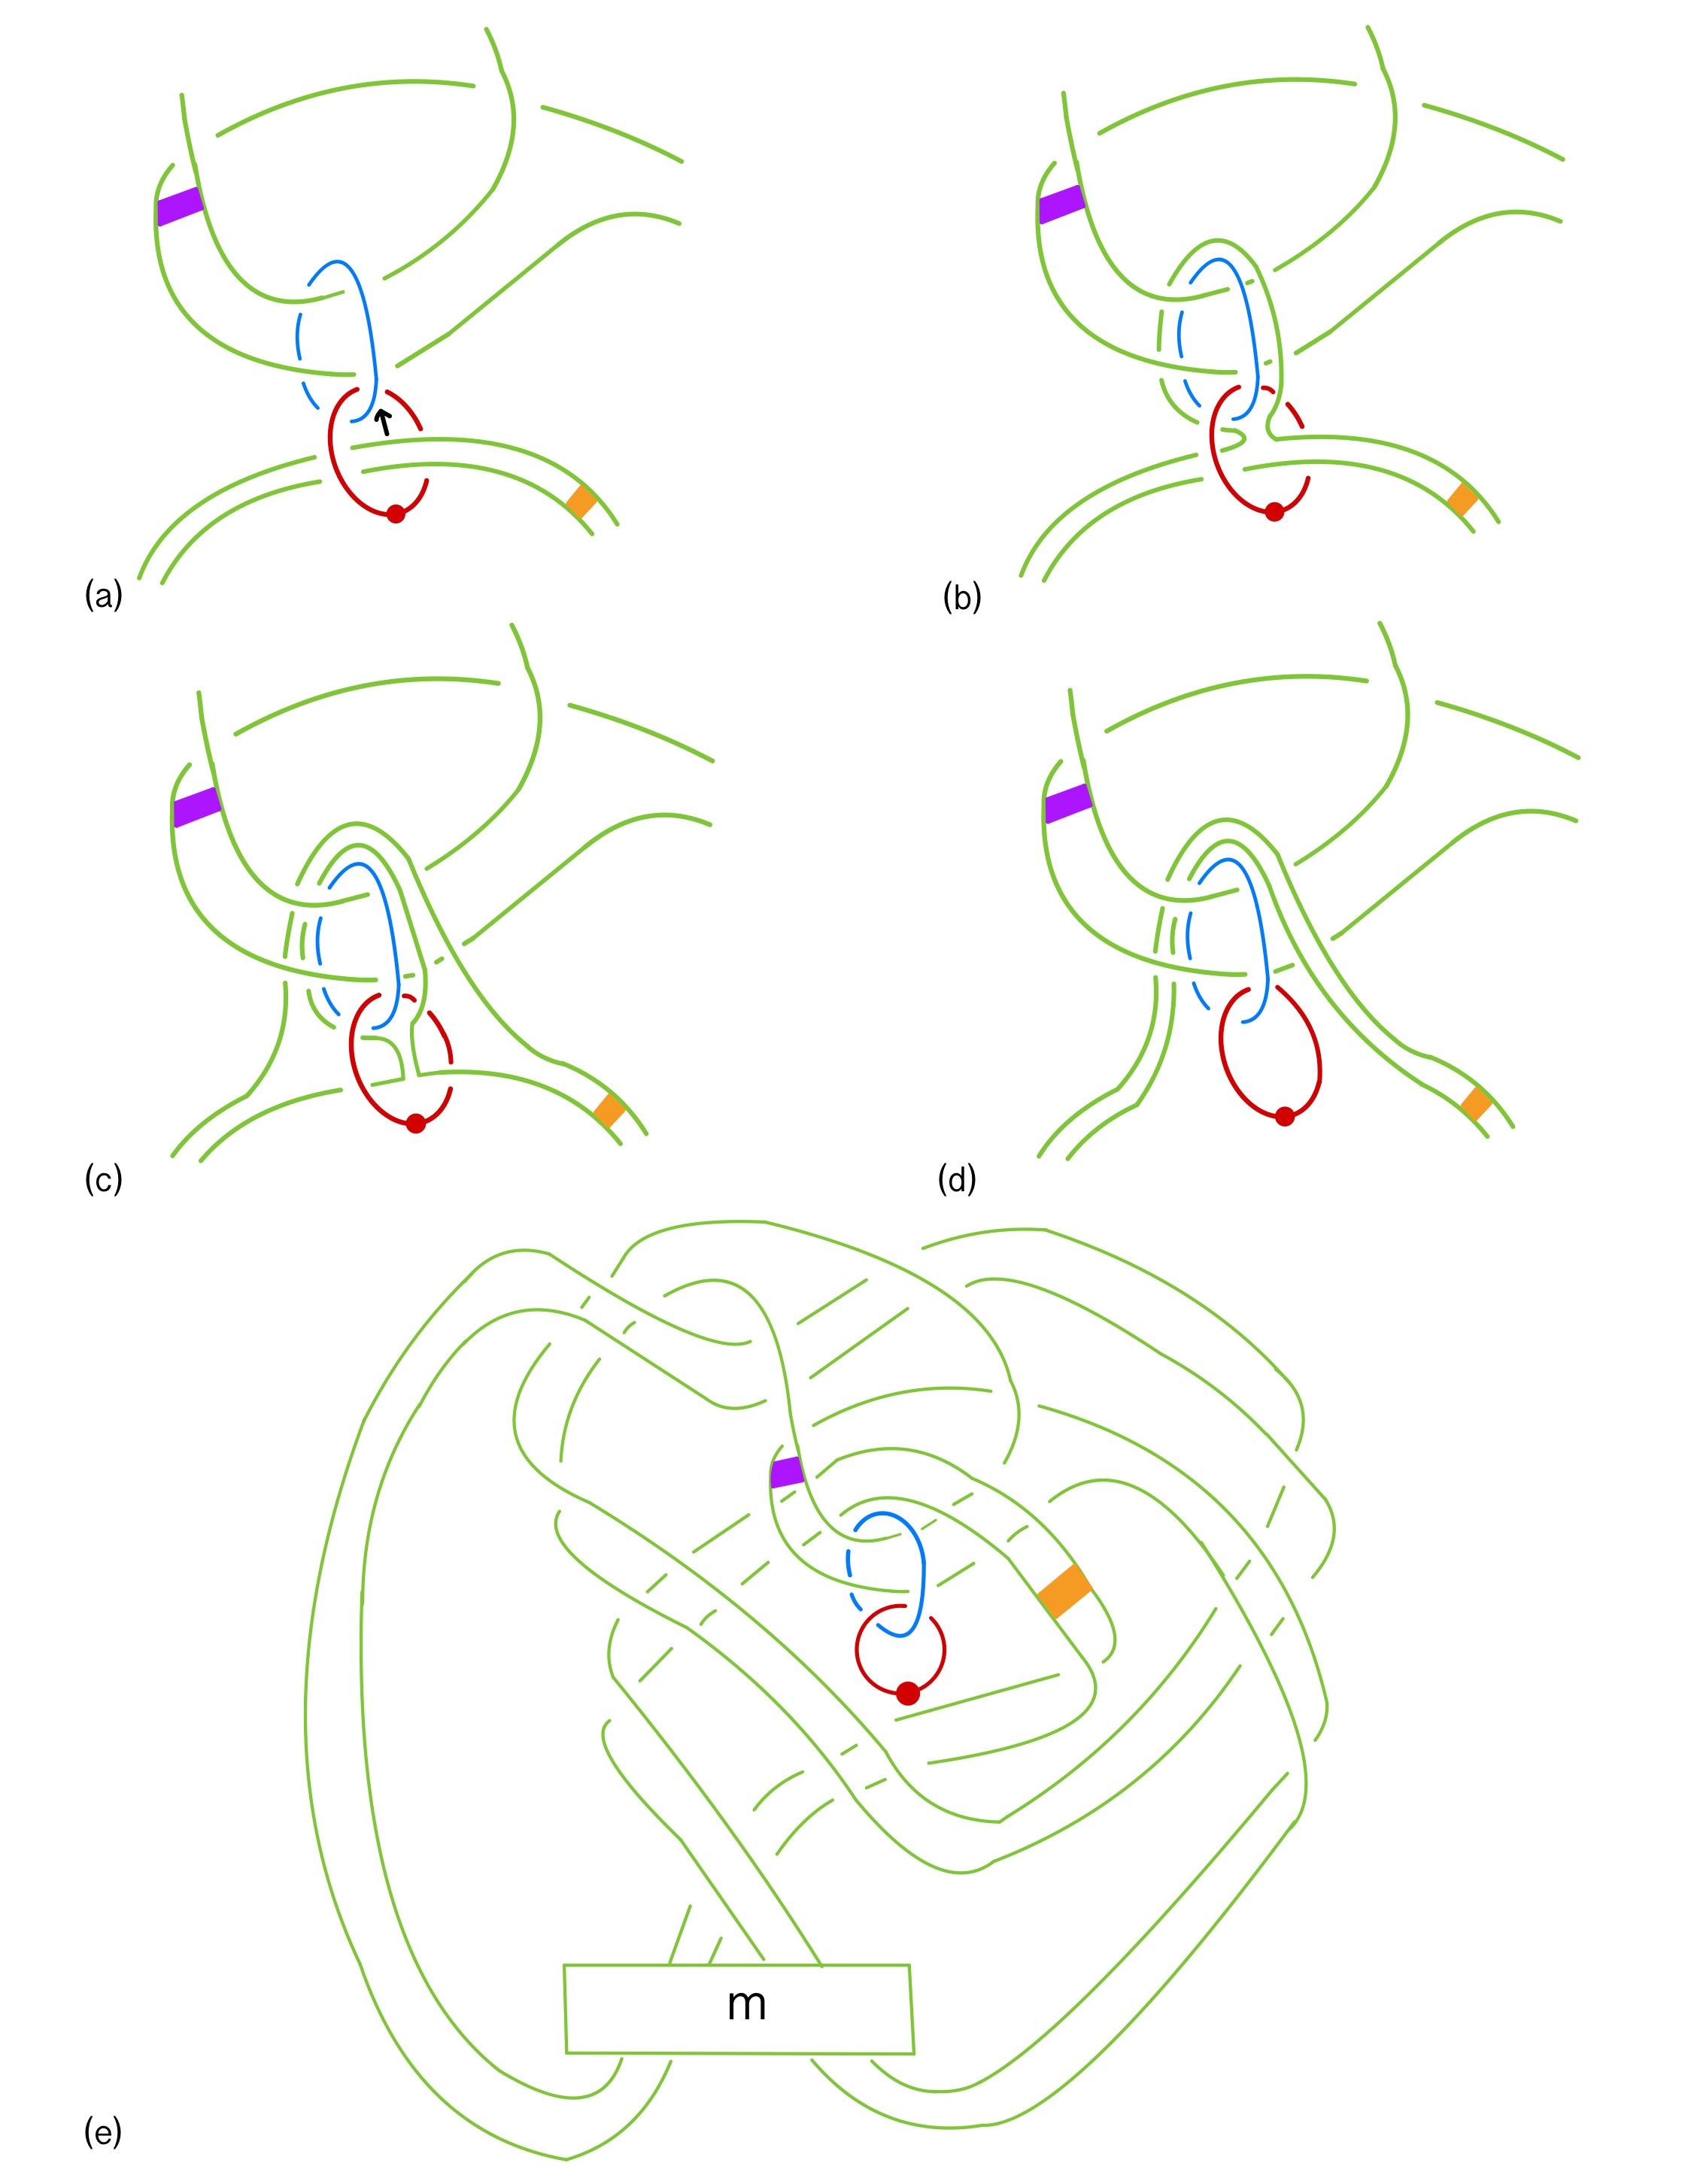
\includegraphics[scale=0.2]{figures/triv5.jpeg} 
    \caption{Handle slides} 
    \label{fig:triv5} 
\end{figure}
Finally, we cancel the handle pair. Figure \ref{fig:km} shows $K_m$ sitting inside the standard diagram of $\s^3$. It is decorated with an orange band and a purple band, which define $D$ and $D'$, respectively. We also depict a knot $J$ in the exterior of $K_m$, which will be used later on.
\begin{figure}[H]
    \centering
    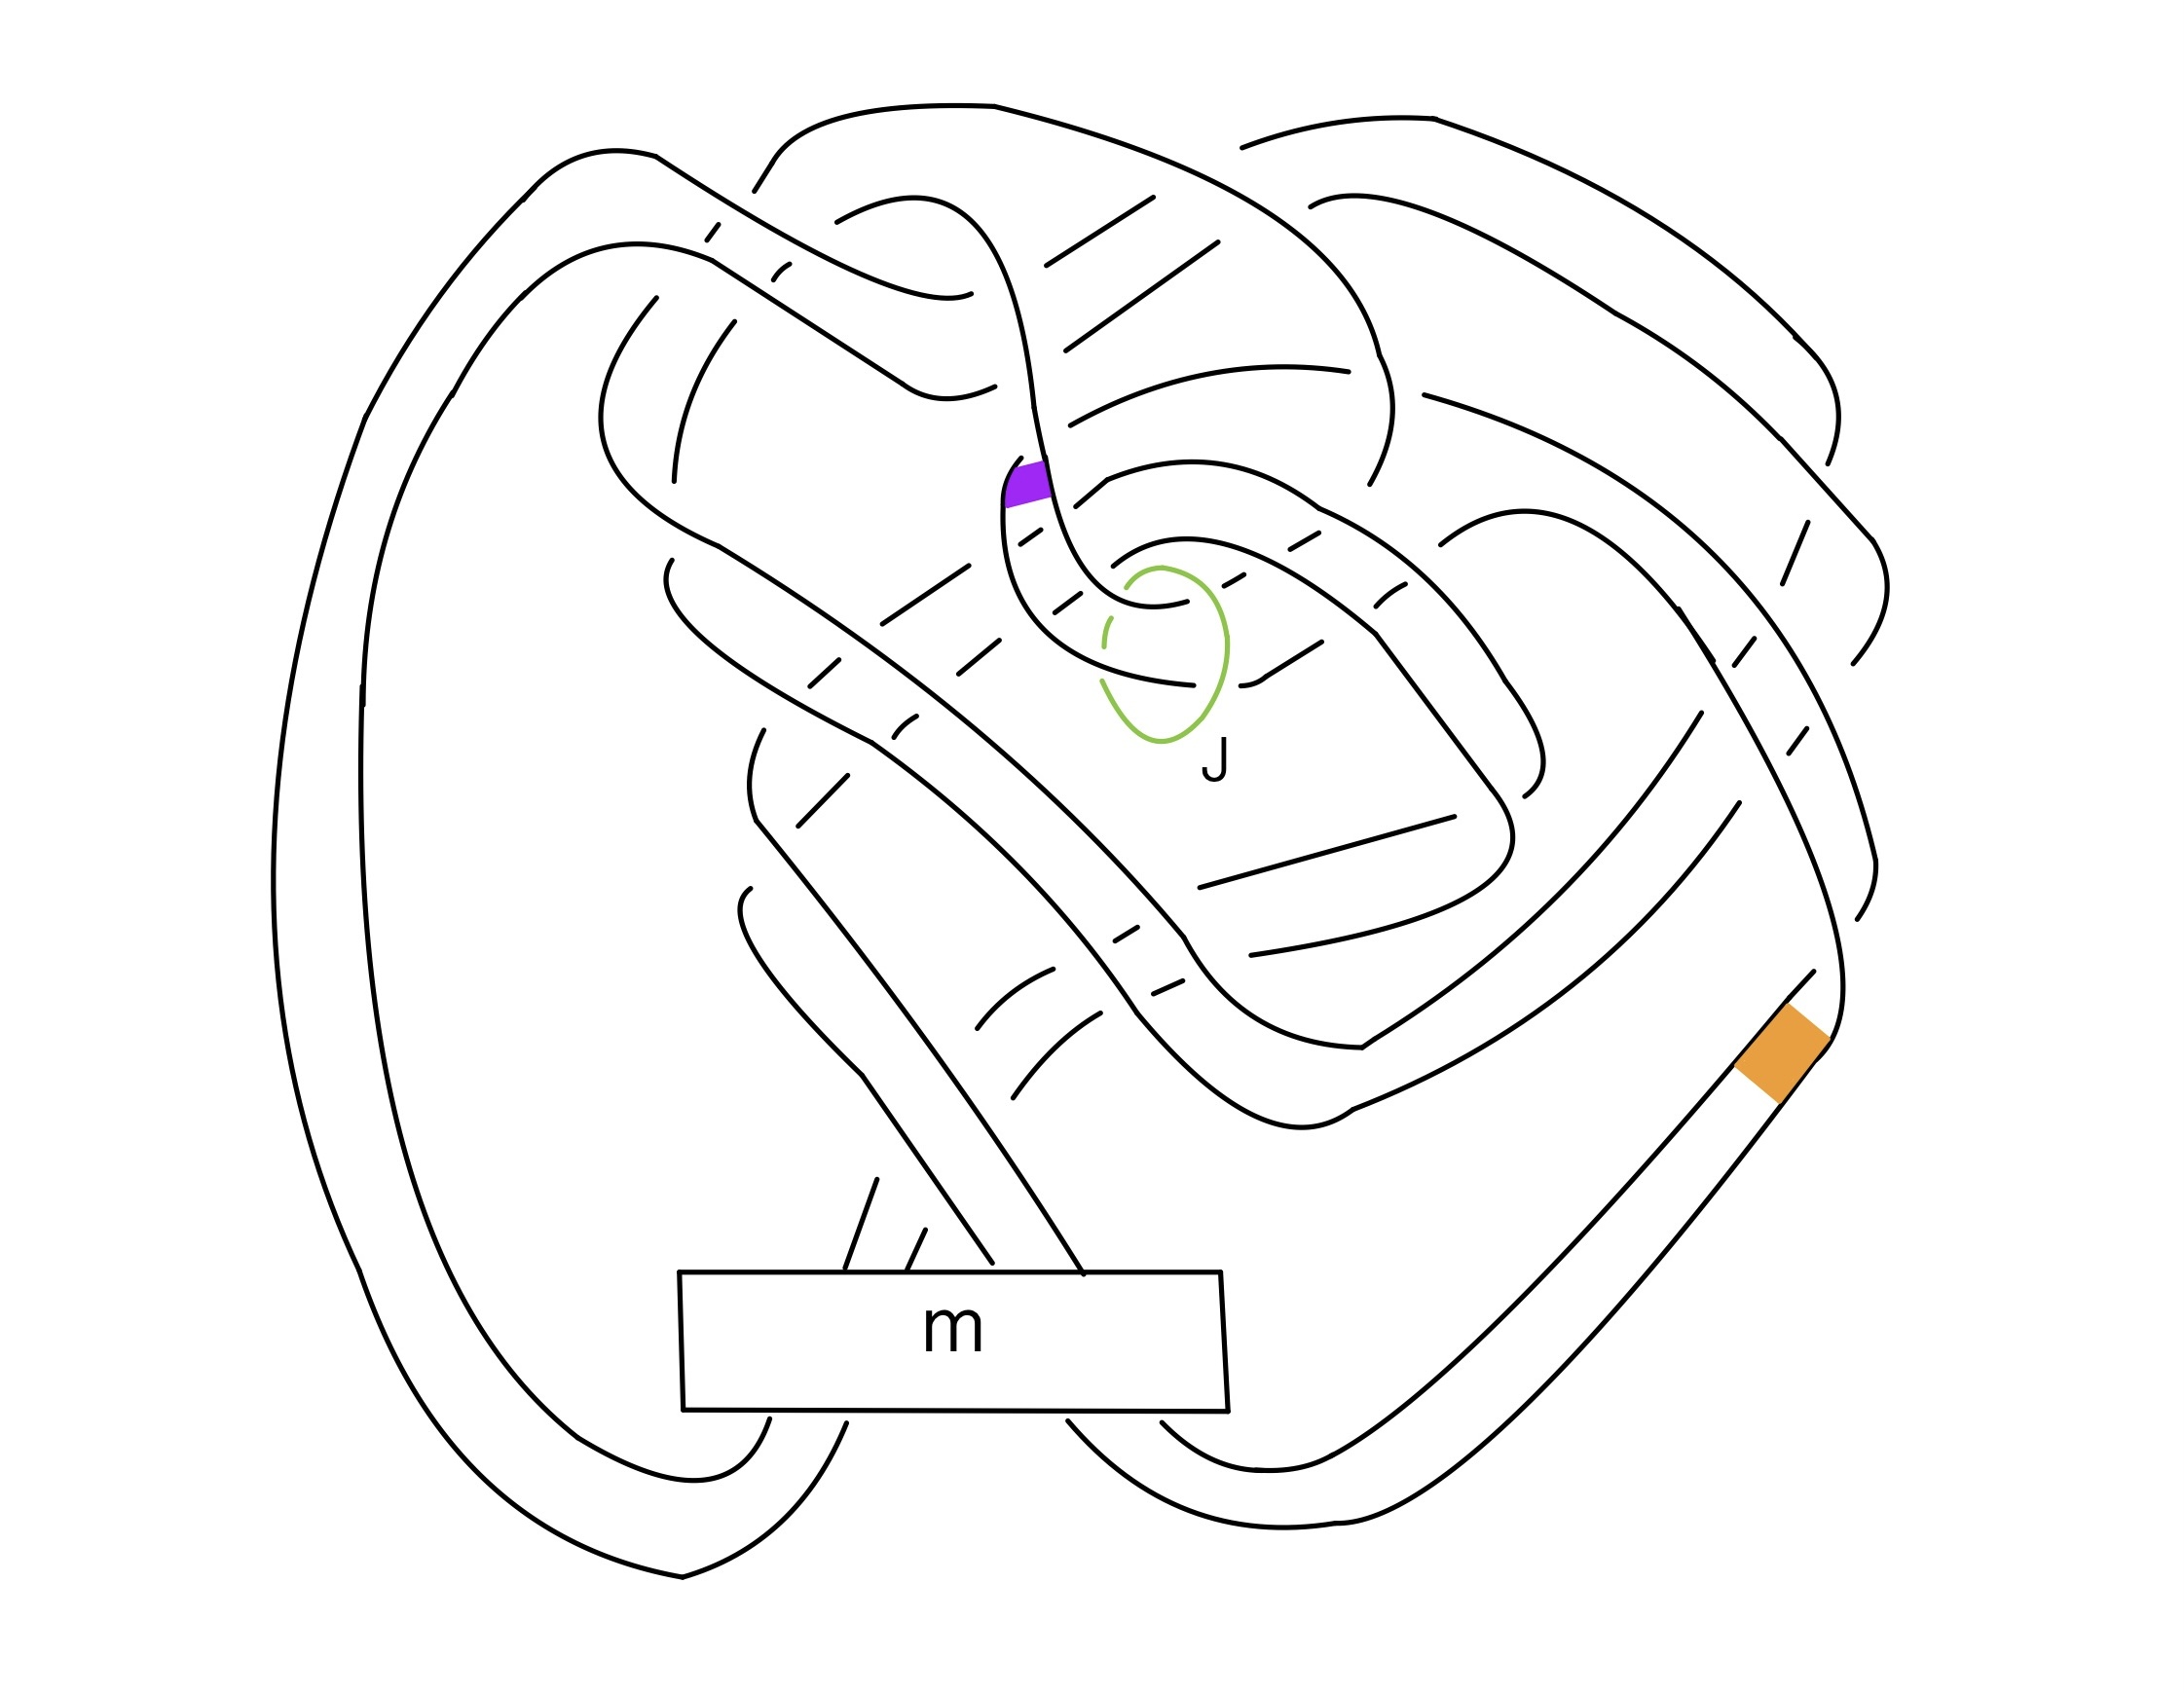
\includegraphics[scale=0.2]{figures/km.jpeg}
    \caption{The knot $K_m$ in $\s^3$, with two bands corresponding to the ribbon structure of $D$ and $D'$}
    \label{fig:km}
\end{figure}
The proof of Theorem \ref{prince} is divided into three steps. \\
(A) $D$ and $D'$ are smoothly isotopic to symplectic disks, \\
(B) $D, D'$ are topologically isotopic, \\
(C) $D, D'$ are not smoothly isotopic. \\ 
\newpage
\textbf{Proof of A} \\
Our goal is to construct a positively transverse link movie\footnote{For background, we refer the reader to \cite{lickorish1997introduction}, \cite{geiges2008contact}} to apply the following Lemma.
\begin{lem}\label{cob}Let $S \subseteq\B^4$ be a properly embedded surface, presented by a sequence of transverse links in $(\s^3, \xi_{st})$ related by the moves depicted in Figure \ref{fig:moves} and transverse isotopy. Then $S$ is smoothly isotopic ,relatively to the boundary, to a symplectic surface in $(\B^4, \omega_{st})$.
\end{lem}
For a proof via ascending surfaces, we refer the reader to \cite{BoileauOrevkov2001} Lemma 1, (cfr \cite{Hayden_2021}). 
\begin{figure}[H]
    \centering
    
\includegraphics[scale=0.2]{figures/moves.jpeg}
    \caption{Elementary birth (a) and saddle (b) moves between transverse link diagrams}
    \label{fig:moves}
\end{figure}
Figure \ref{fig:tra}(b) is a transverse representative of $K_m$ because it is the transverse pushoff of a Legendrian realization \ref{fig:tra}(a) 
\cite{geiges2008contact}.
\begin{figure}[H]
    \centering
    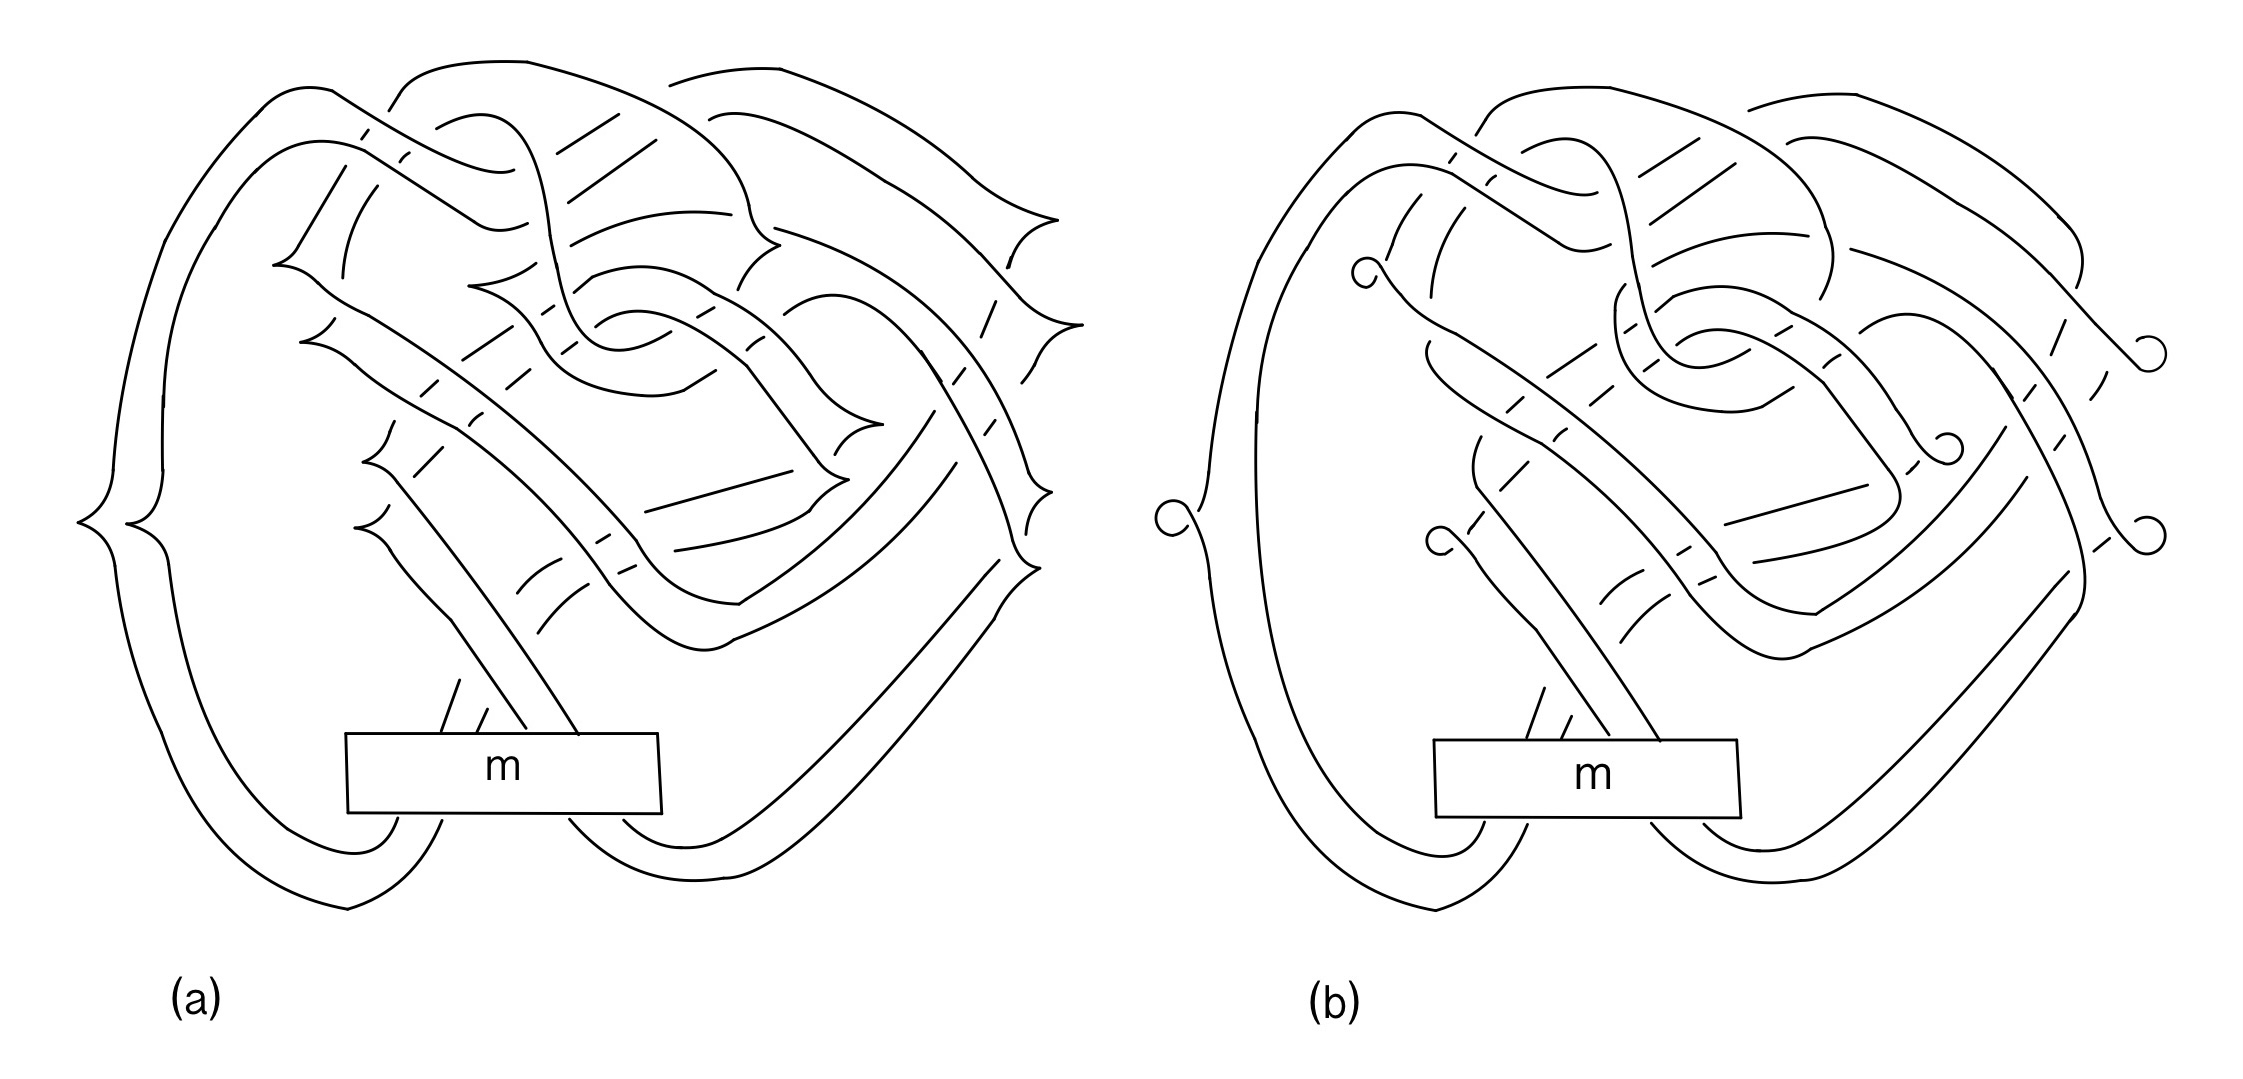
\includegraphics[scale=0.18]{figures/tra.jpeg}
    \caption{Legendrian (a) and transverse (b) representatives of $K_m$}
    \label{fig:tra}
\end{figure}
\begin{figure}[H]
    \centering
    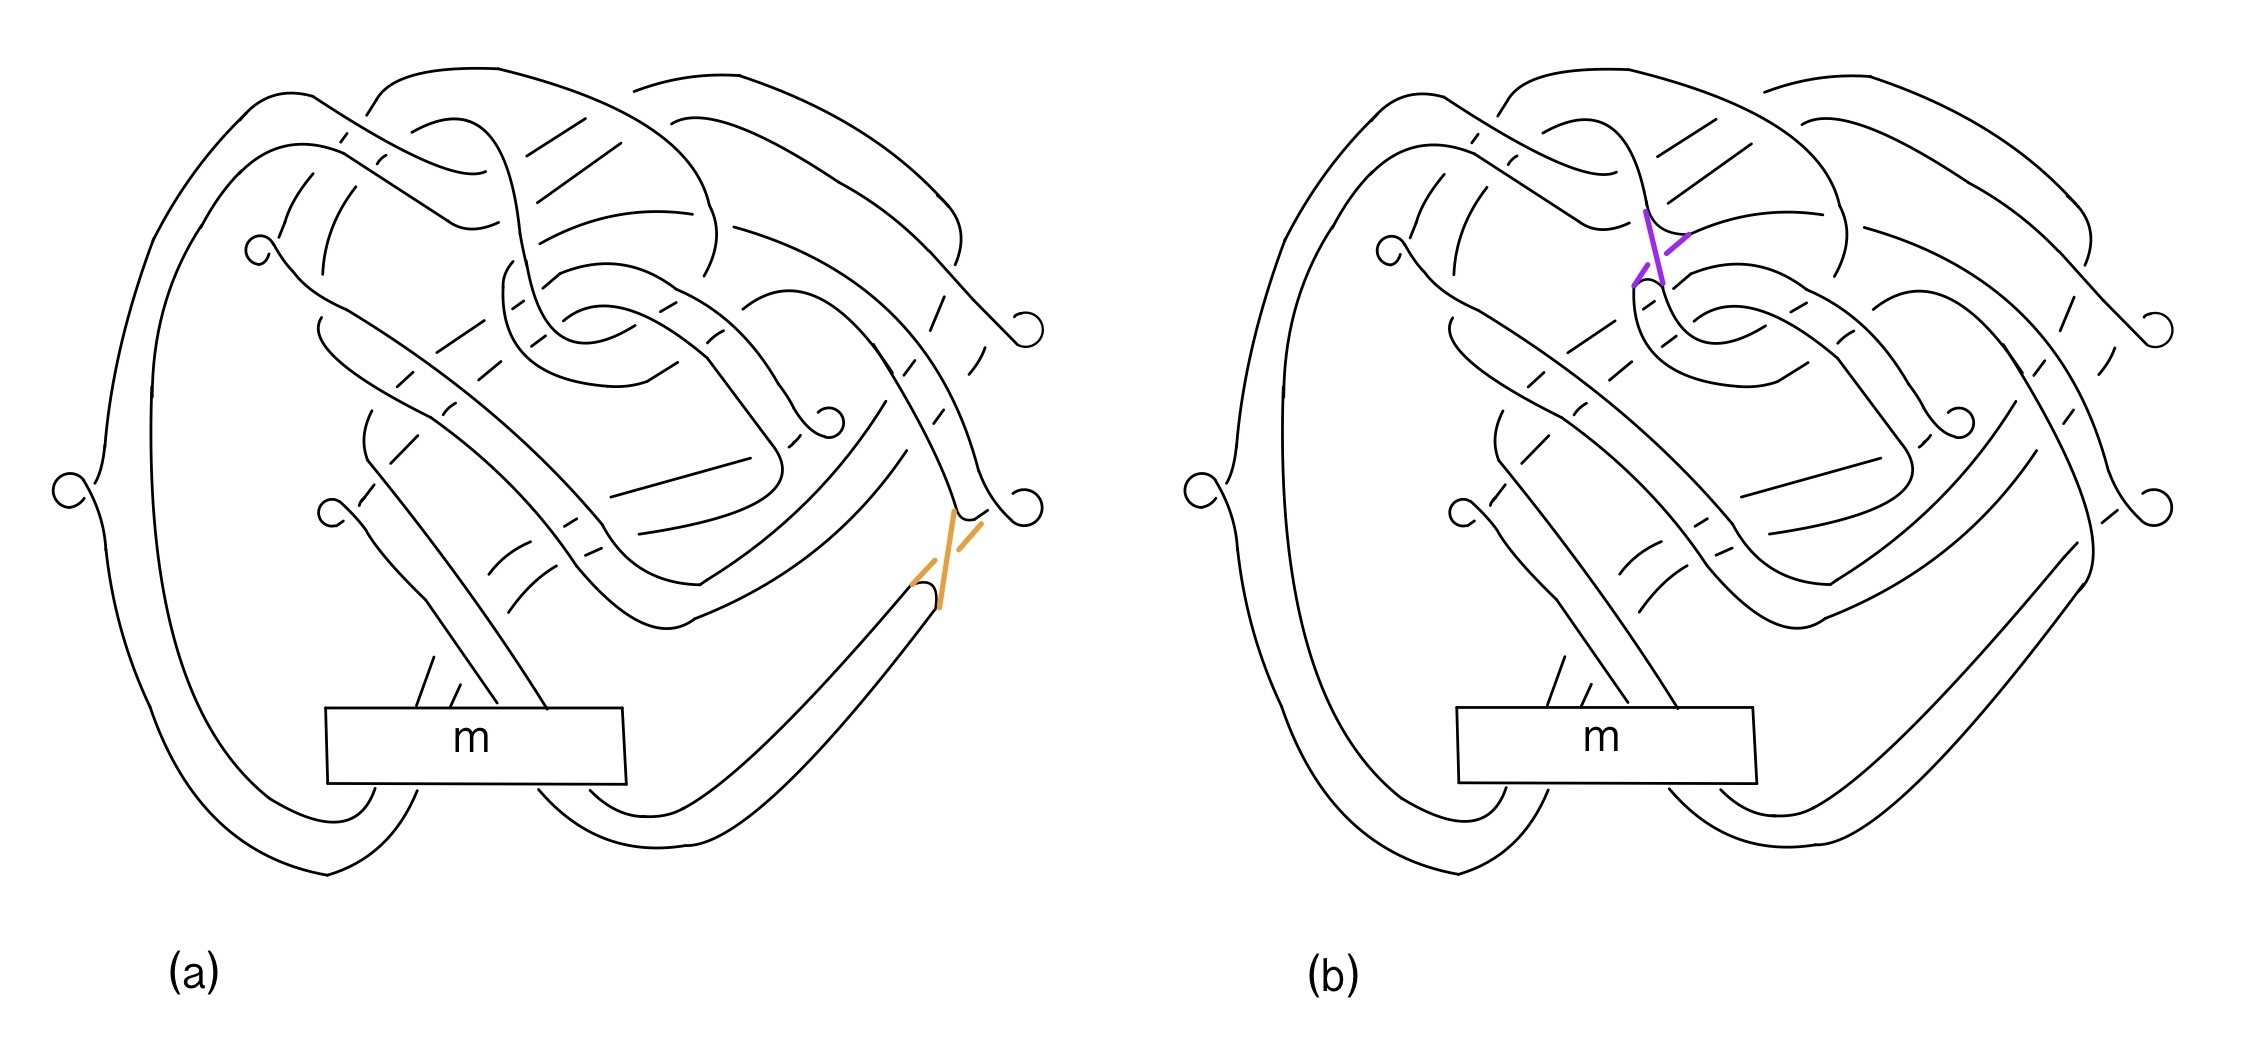
\includegraphics[scale=0.18]{figures/band.jpeg}
    \caption{Saddle moves on transverse link diagrams}
    \label{fig:band}
\end{figure}
Moreover, the band moves depicted in Figure \ref{fig:band} corresponds to the previous band surgeries. These moves are also cobordisms between $K_m$ and a pair of positively transverse unknots. Thus, using Lemma \ref{cob}, we construct symplectic disks which are smoothly isotopic to $D$ and $D'$.
\\ \\
\textbf{Proof of B} \\
To establish the topological isotopy, we use a result of Conway and Powell.
\begin{defn}A ribbon disk $D$ is $\Z$-homotopy ribbon, if $$
\pi_1(\B^4 \setminus \nu(D)) \cong \Z
$$
An oriented knot is $\Z$-homotopy ribbon, if it bounds a $\Z$-homotopy ribbon disk.
\end{defn}
\begin{thm}\cite{conway-powell}\label{conwa} Any two $\Z$-homotopy ribbon disks of a $\Z$-homotopy ribbon knot, are ambiently topologically isotopic relatively to the boundary.
\end{thm}
We will construct Kirby diagrams for $\estd$ and $\estdi$. The smooth structure of $D$ and $D'$ is defined via the handle decomposition with two minima and one saddle. As explained in sections \ref{driii} \ref{acqua}, we draw a dotted circle on the boundary of each $0$-handle. Then each band corresponds to a $2$-handle of the exterior. The resulting diagrams are depicted in Figures \ref{fig:comp1}(a) and \ref{fig:comp21}(a).
In order to compute the fundamental groups, it is really helpful to isotope the pair of $1$-handles to a two component unlink. The pictures below, illustrate the desired sequence of isotopies and Kirby moves. Observe that step (c) of \ref{fig:comp1} and step (b) of \ref{fig:comp21} involve $1$-handle slides.
Other steps are isotopies.
\begin{figure}[H]
    \centering
    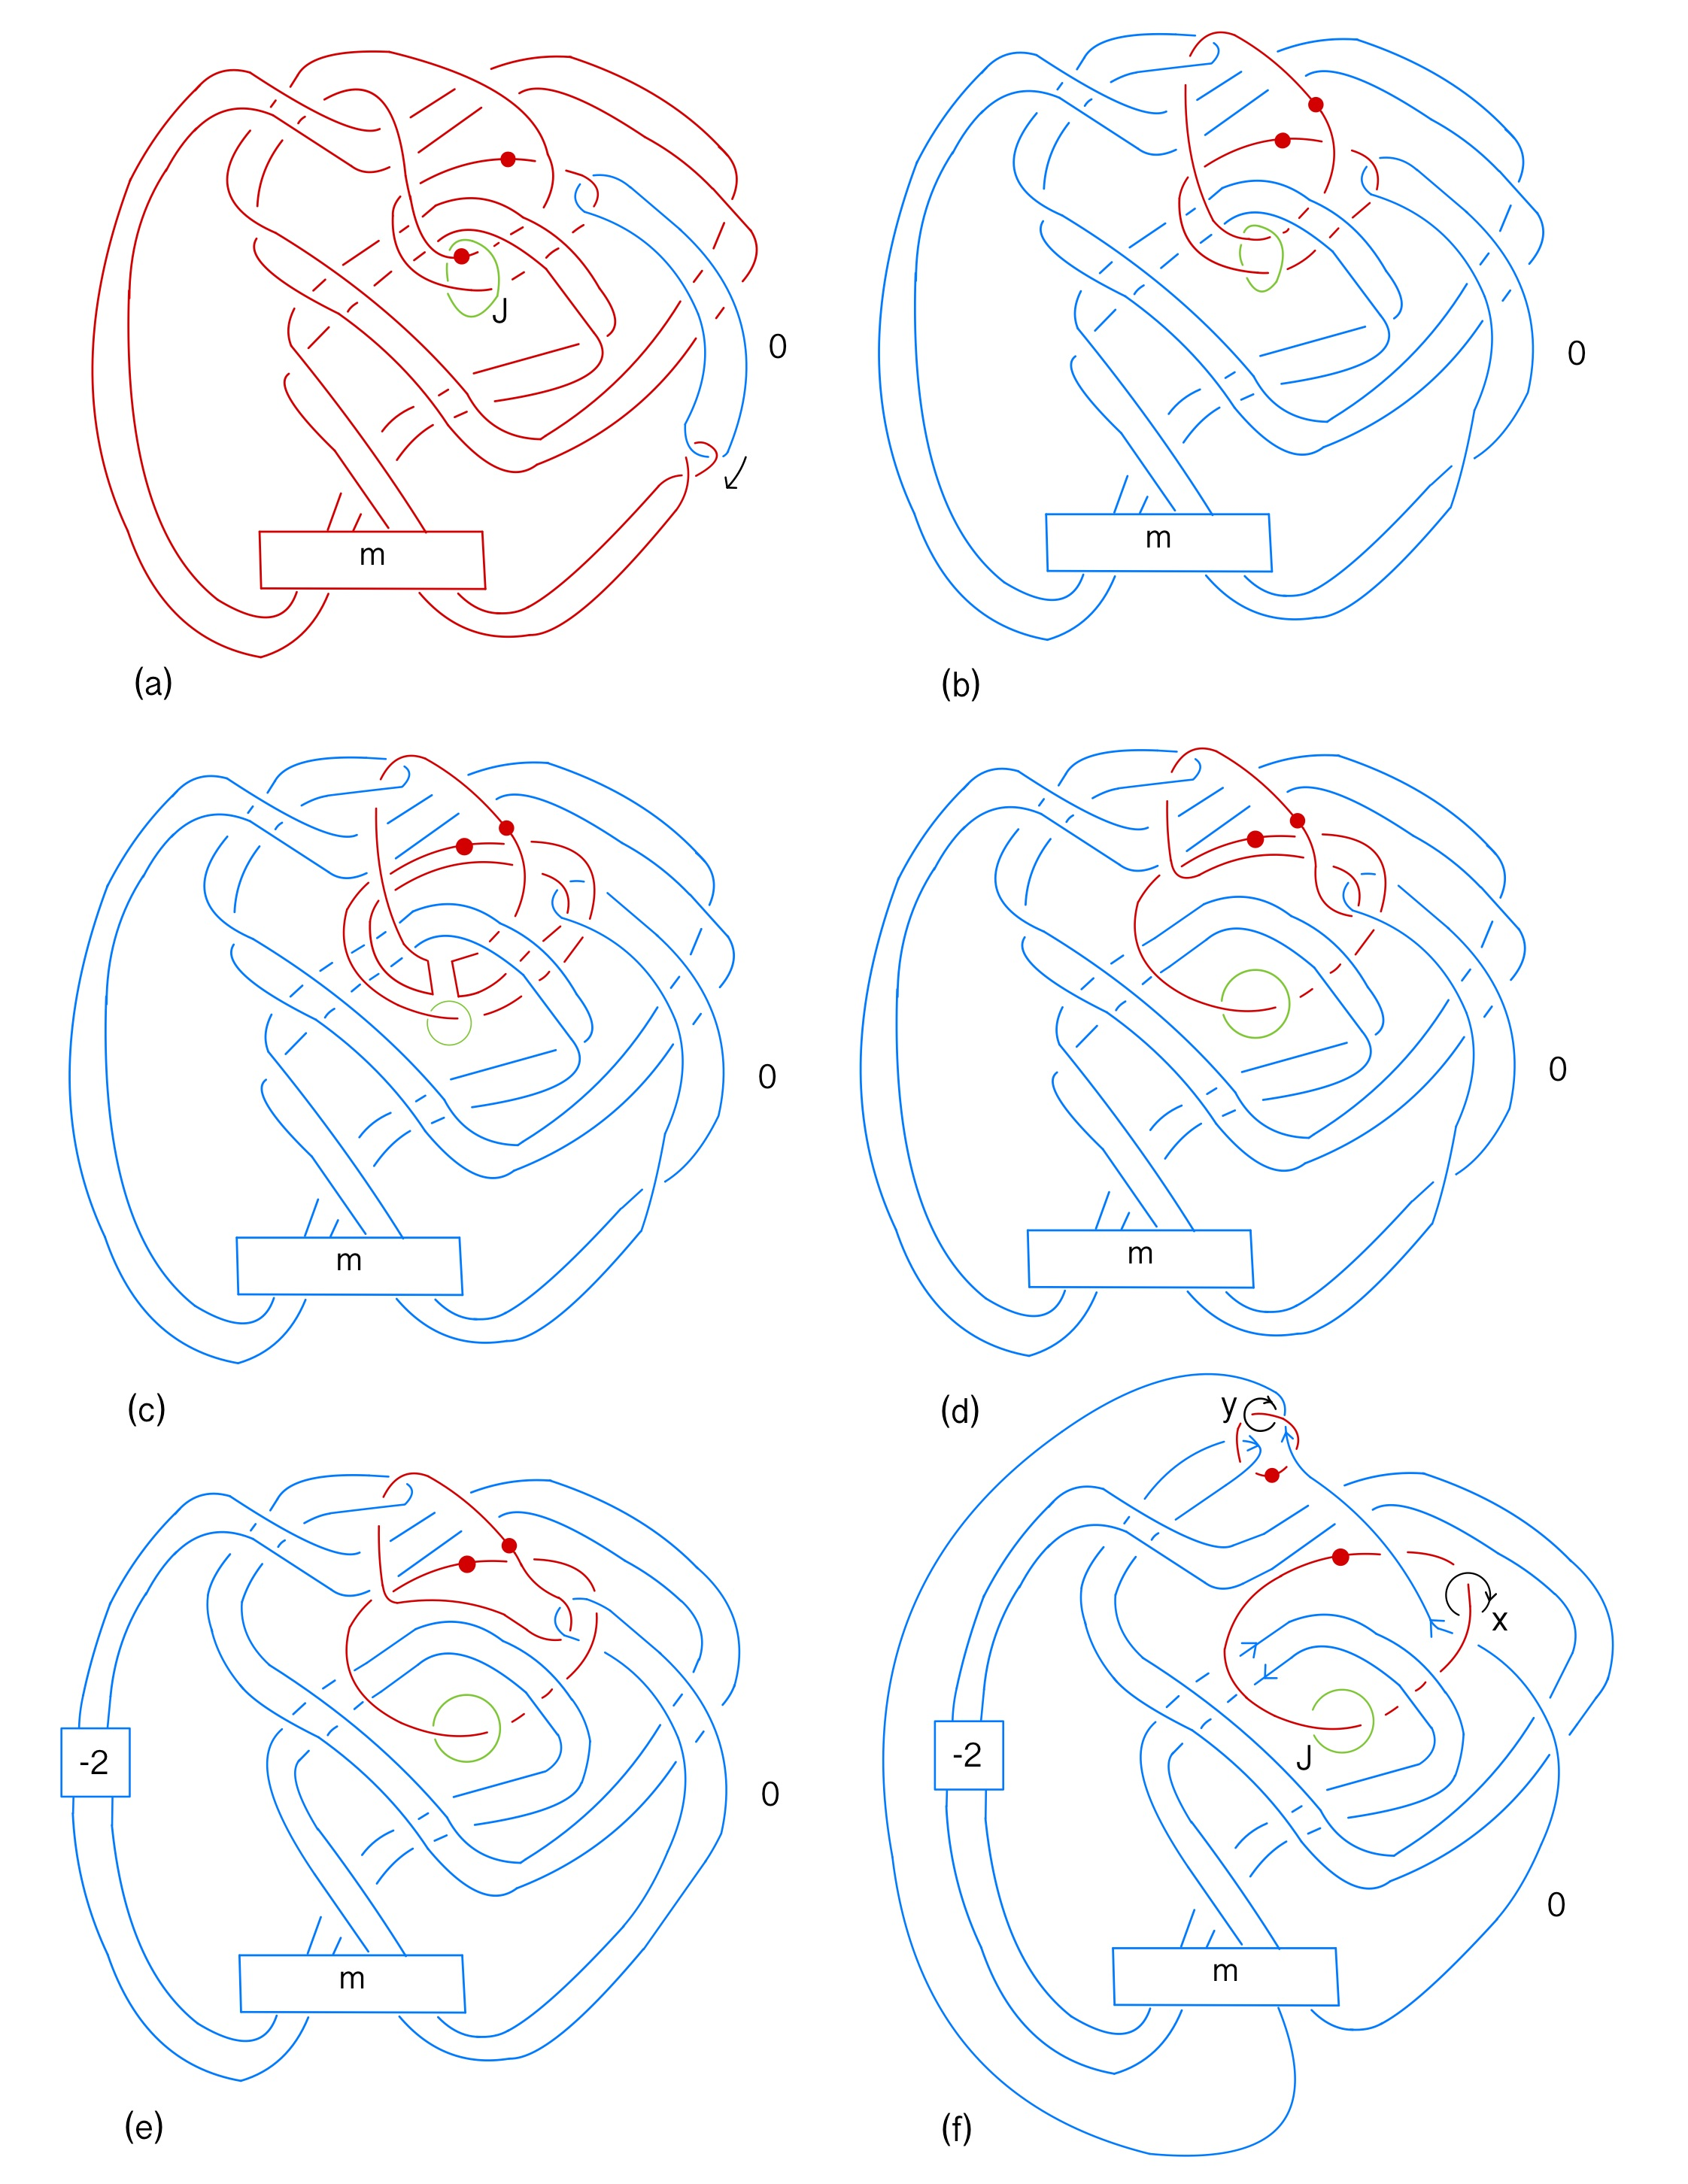
\includegraphics[scale=0.2]{figures/comp1.jpeg}
    \caption{Kirby diagram of $\estd$}
    \label{fig:comp1}
\end{figure}
\begin{figure}[H]
    \centering
    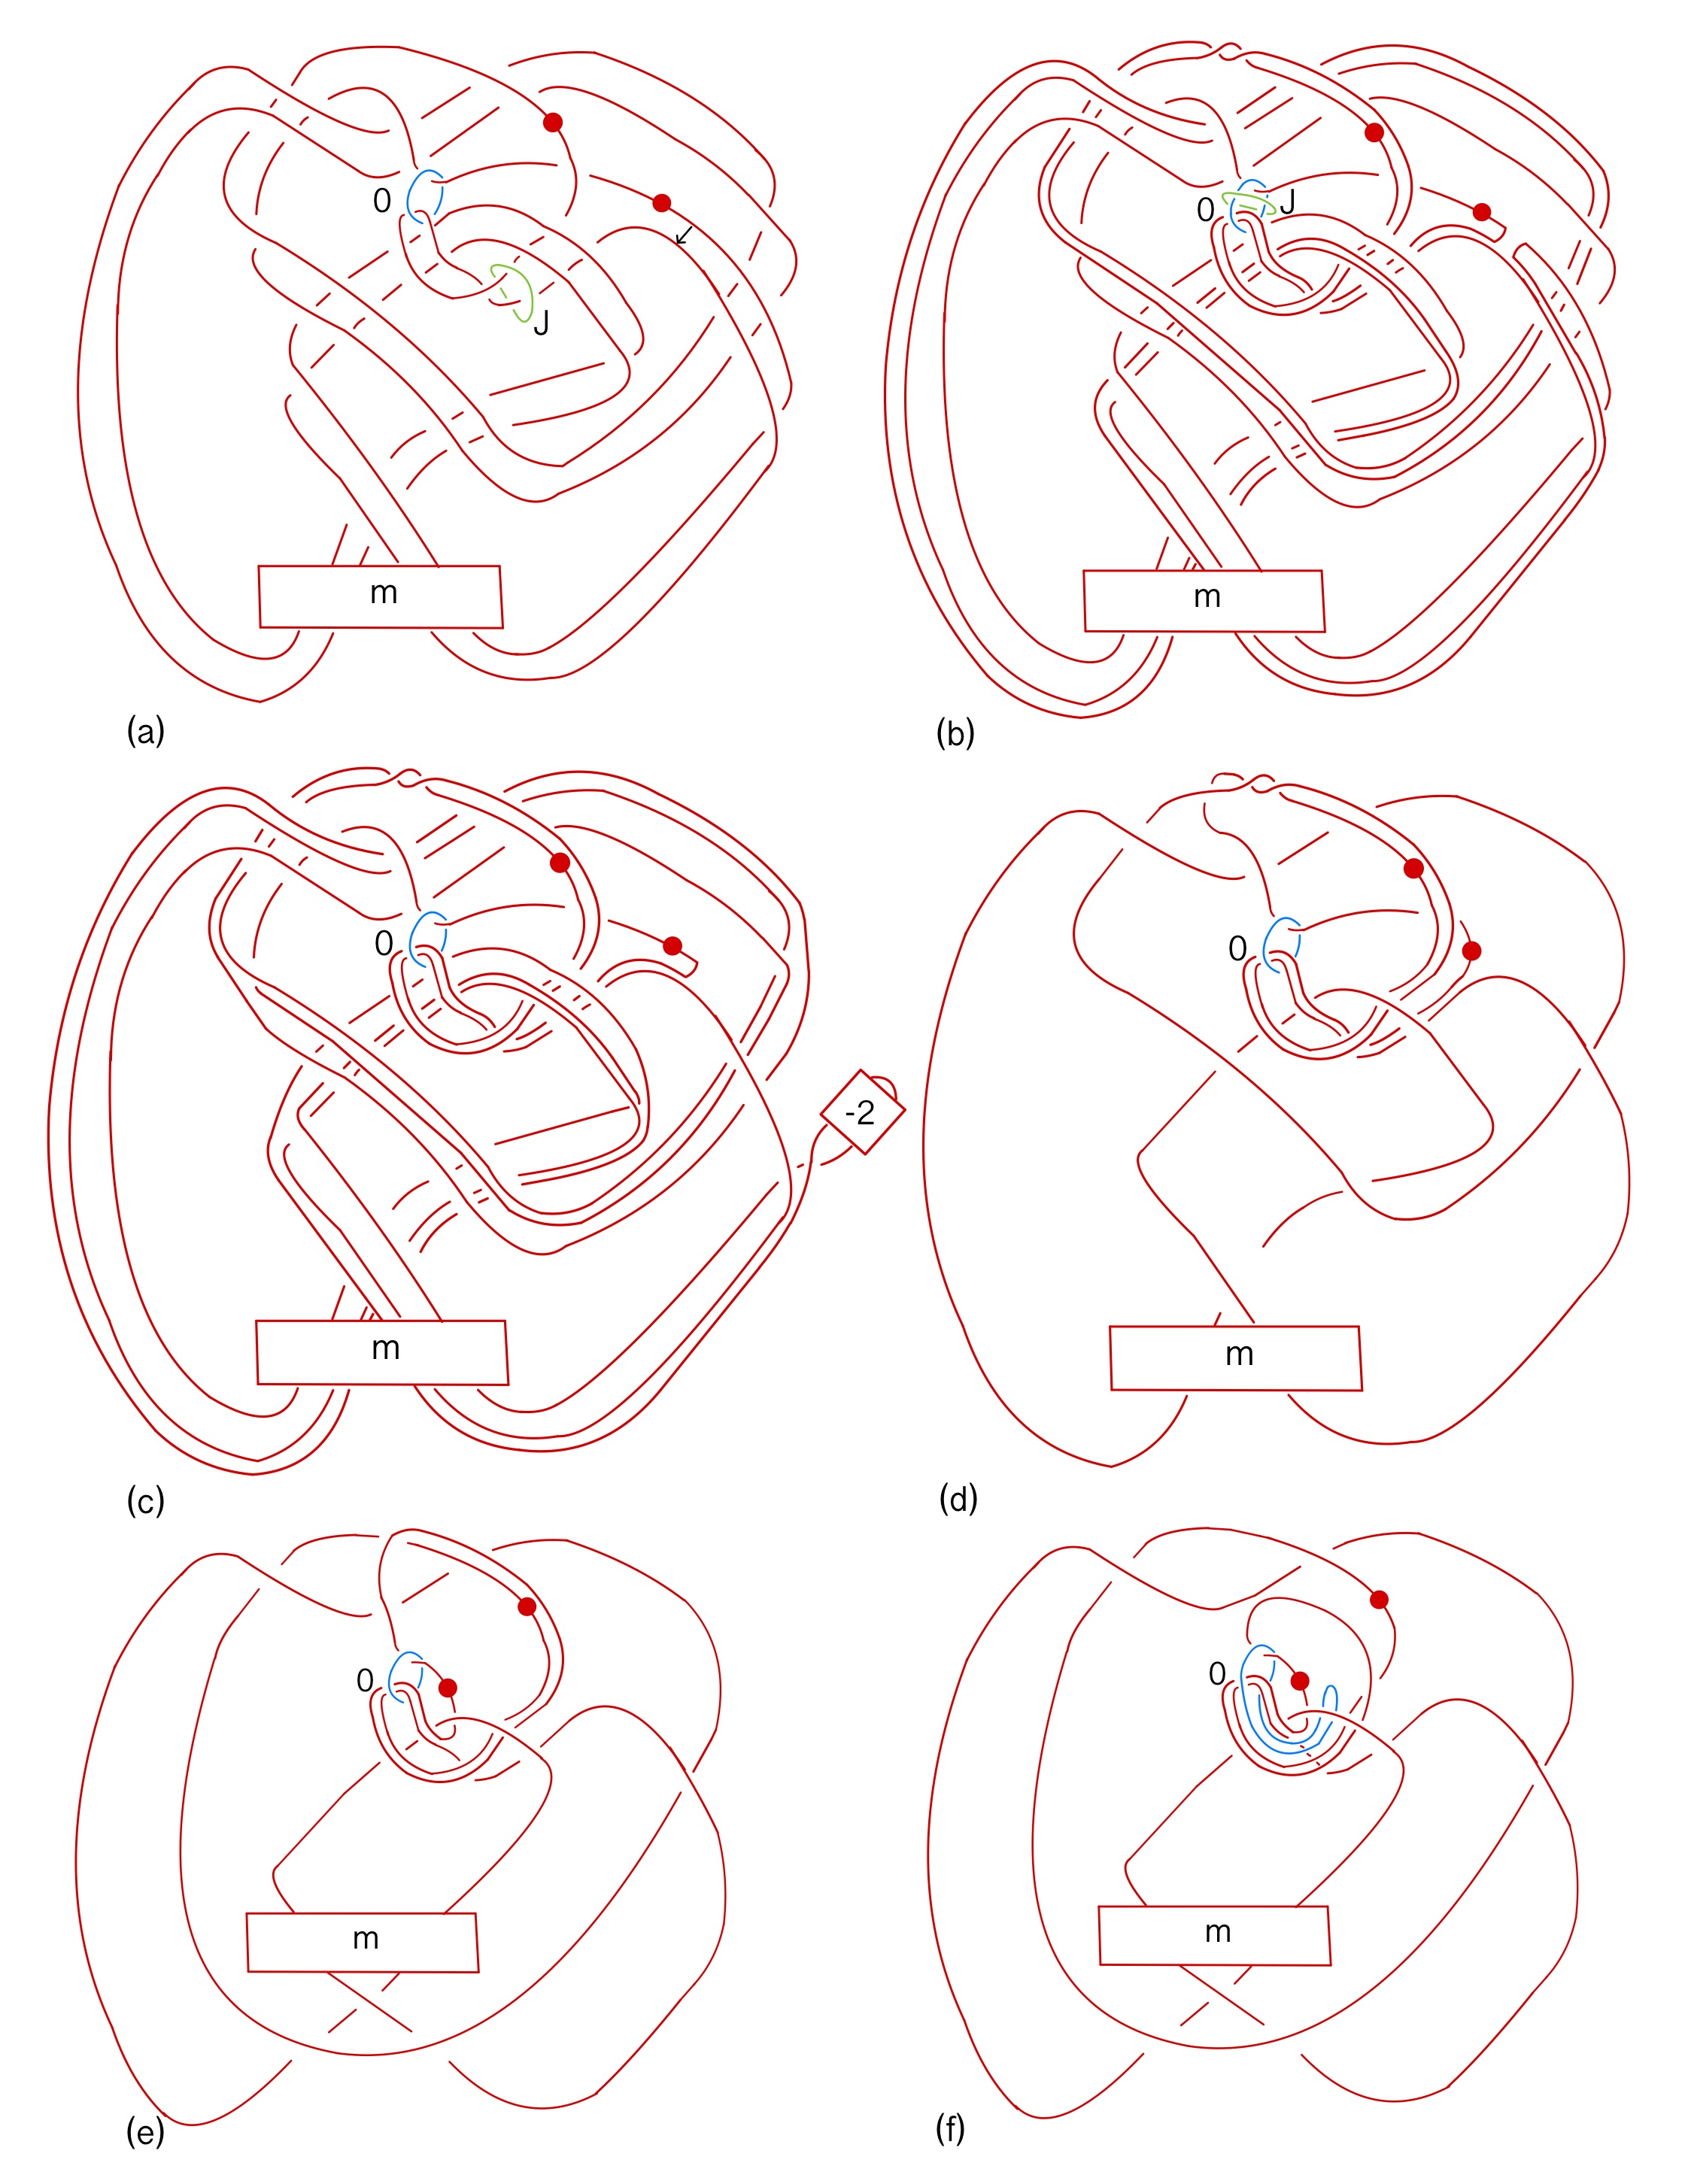
\includegraphics[scale=0.2]{figures/comp21.jpeg}
    \caption{Kirby diagram of $\estdi$}
    \label{fig:comp21}
\end{figure}
\begin{figure}[H]
    \centering
    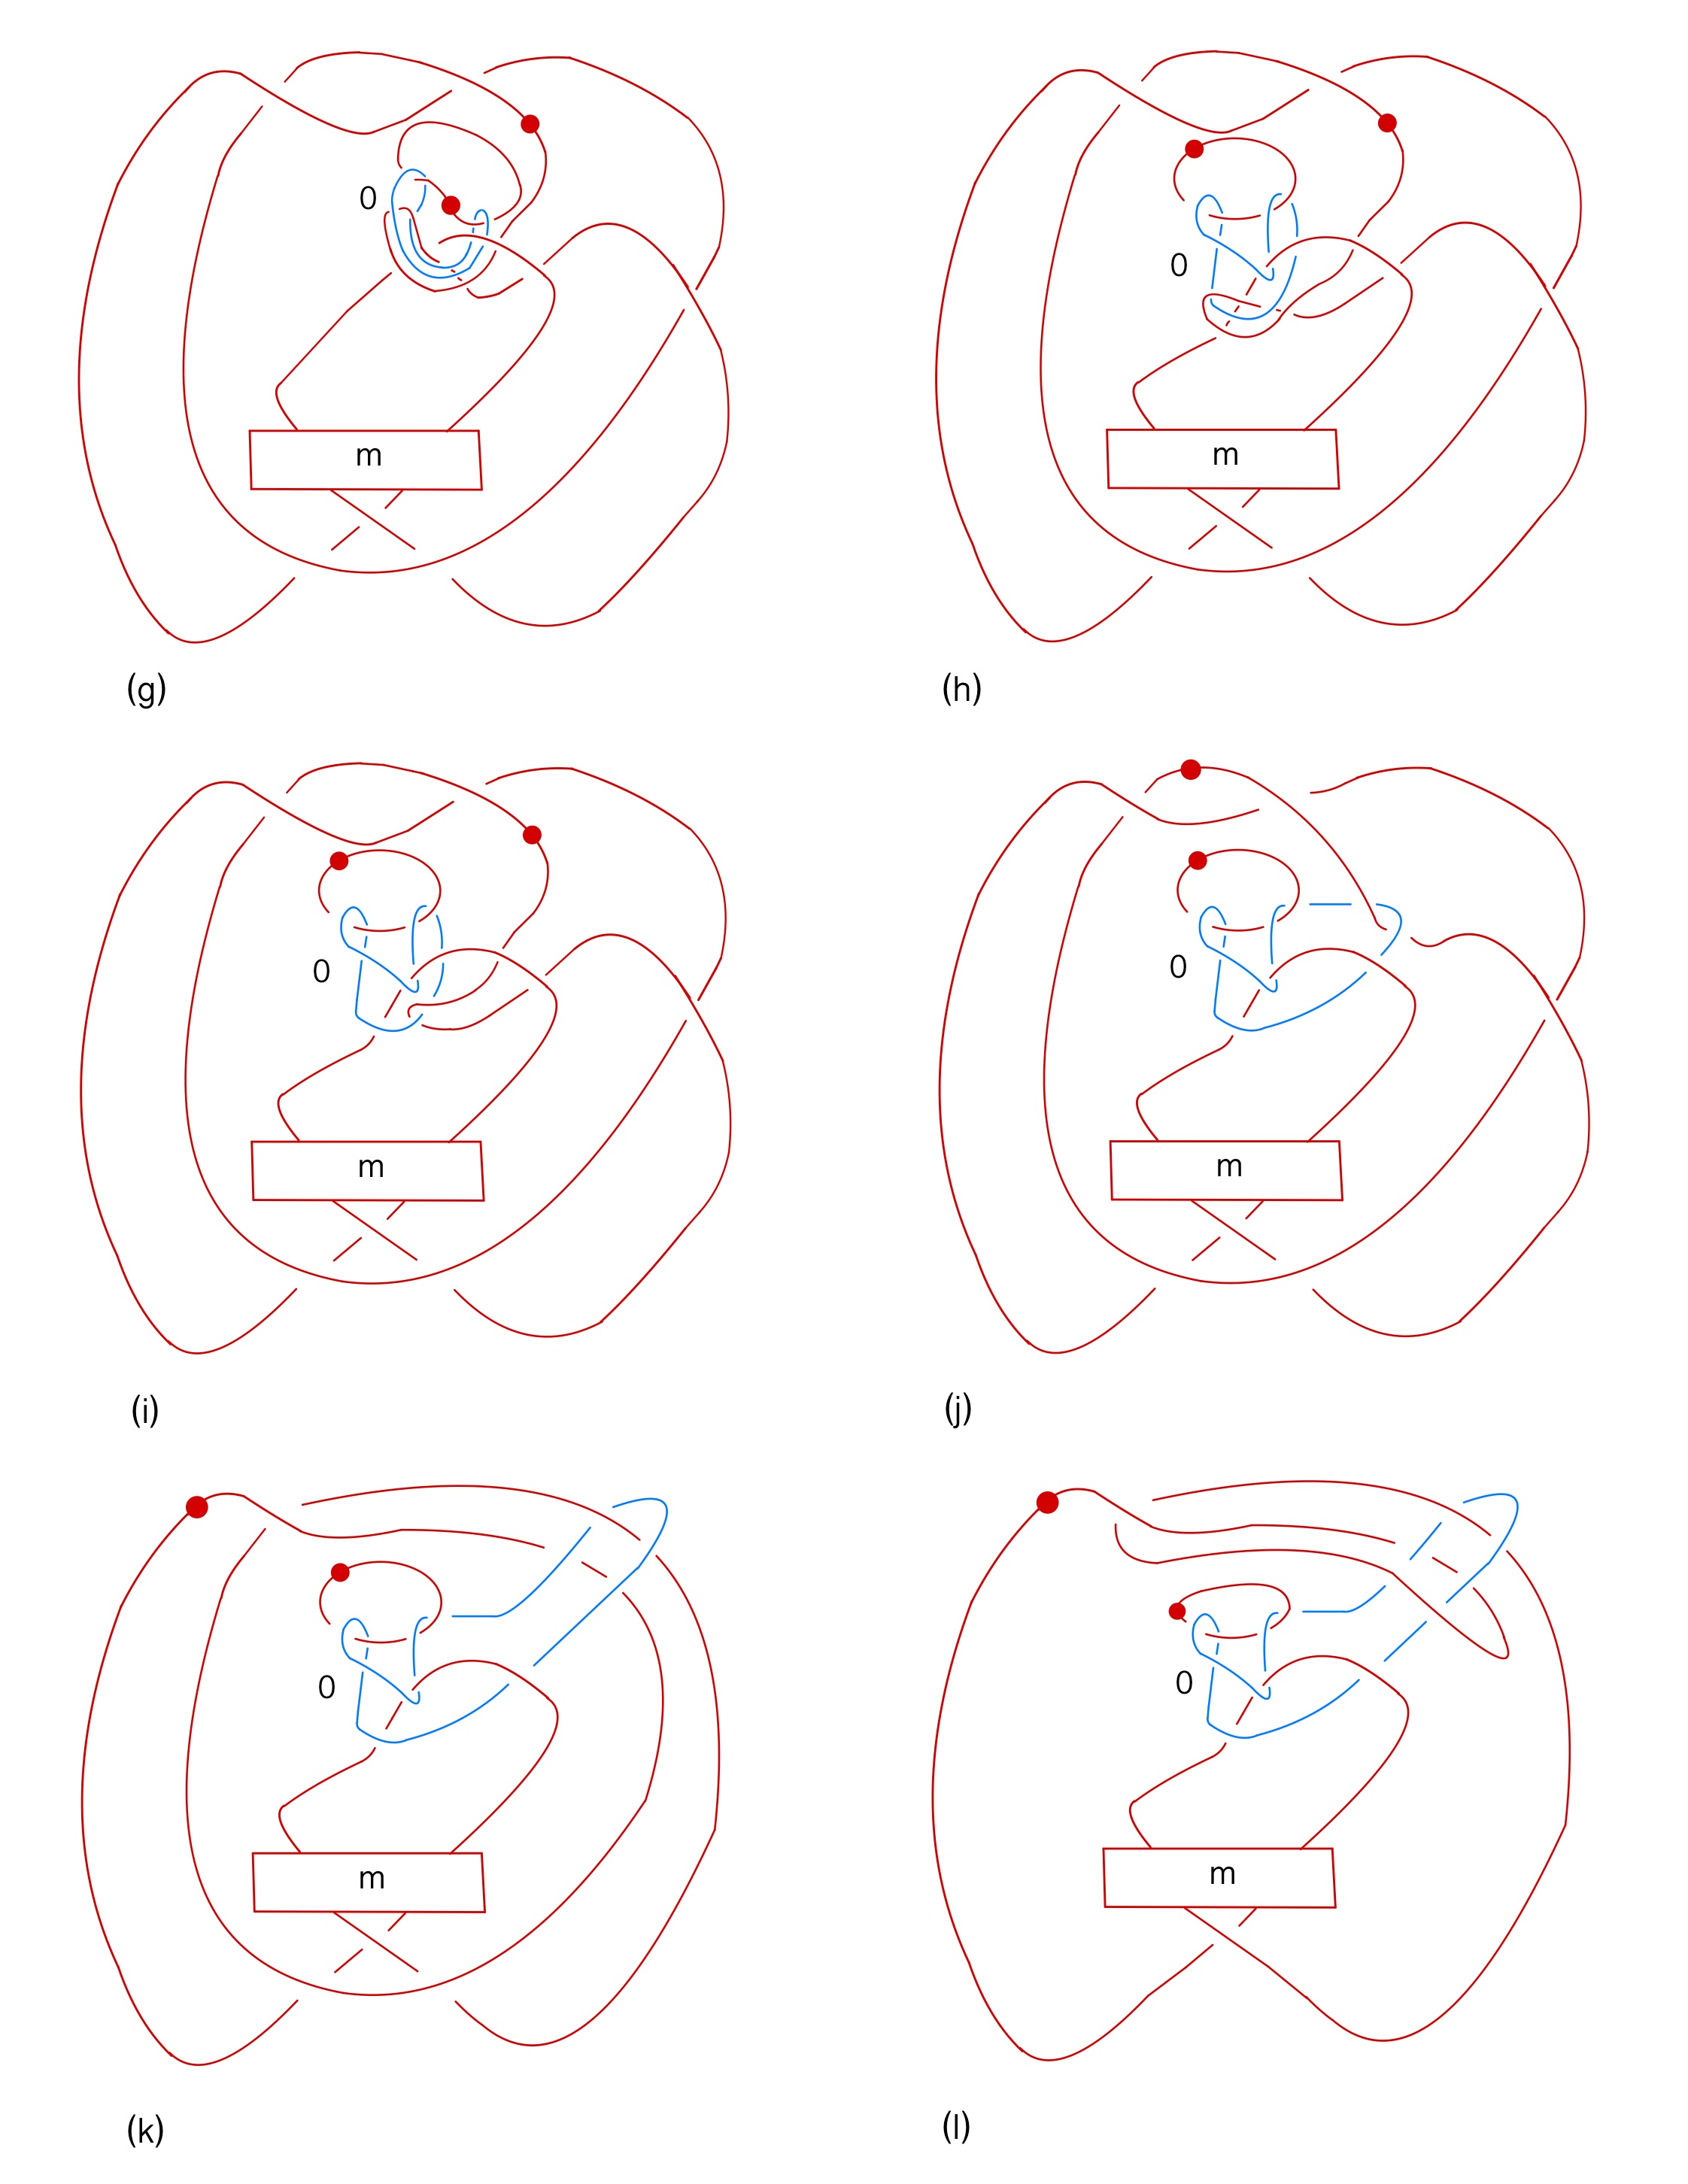
\includegraphics[scale=0.2]{figures/comp22.jpeg}
    \caption{Simplifying the Kirby diagram of $\estdi$}
    \label{fig:comp22}
\end{figure}
\begin{figure}[H]
    \centering
    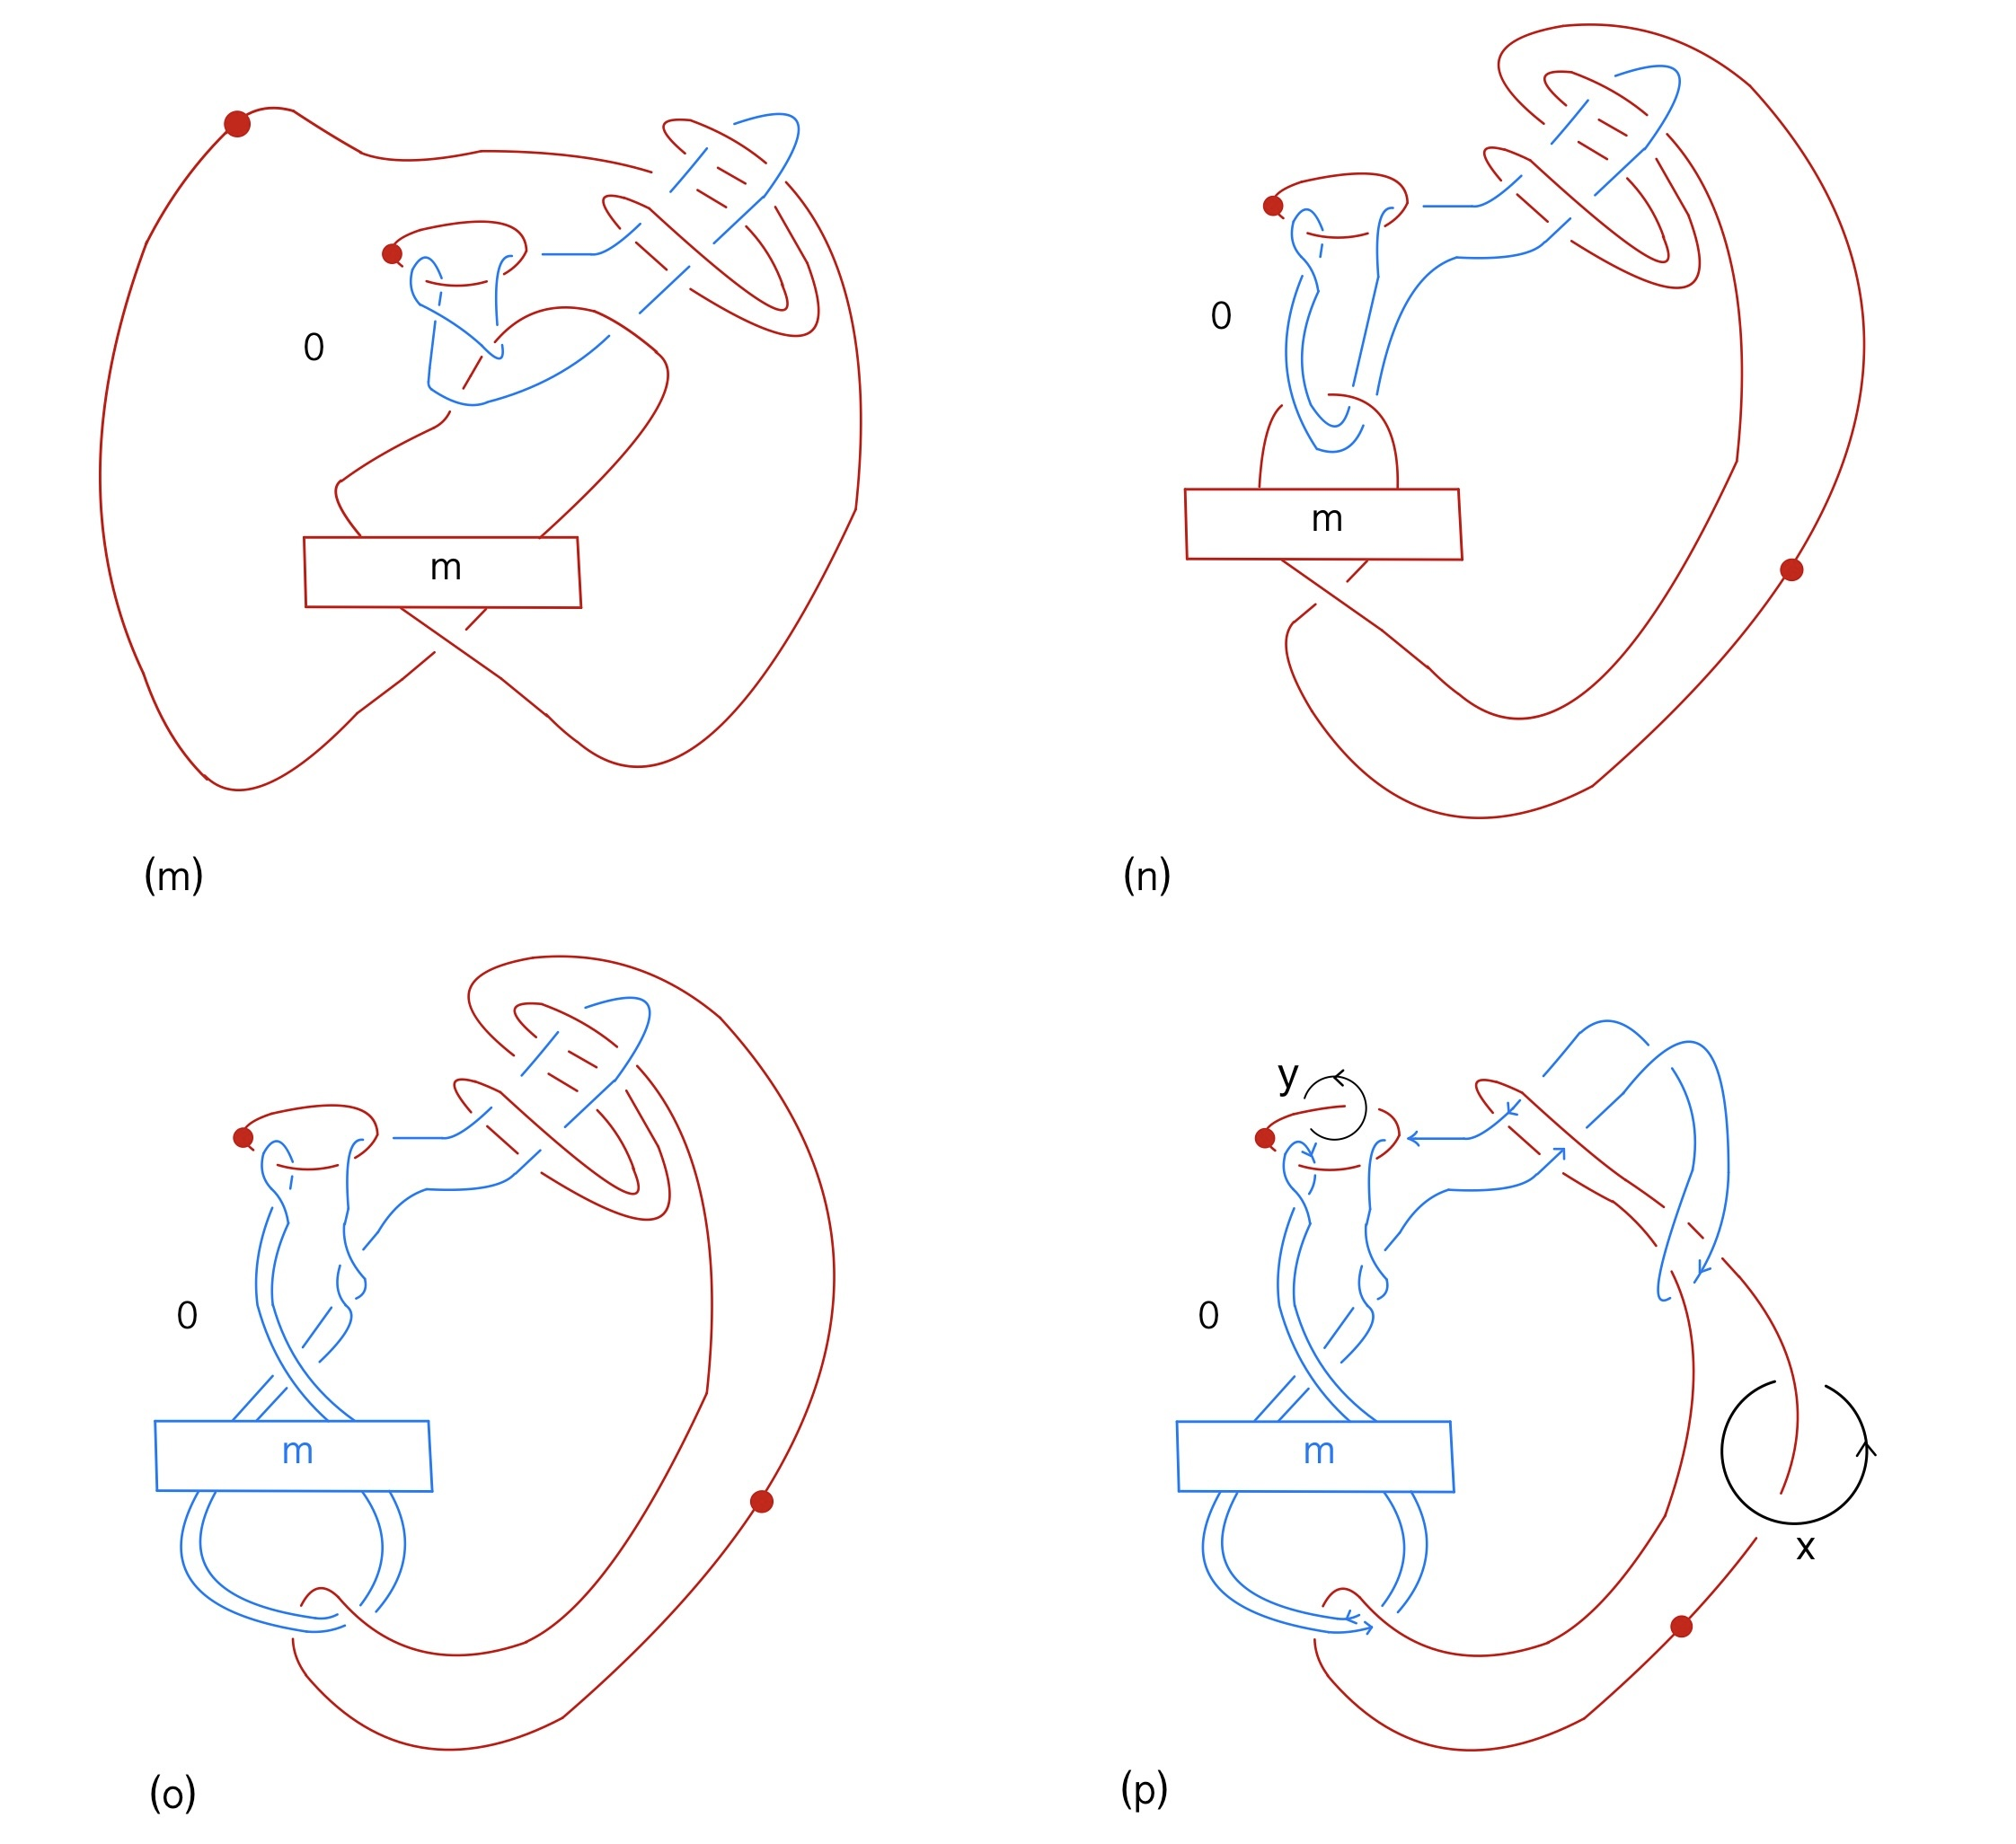
\includegraphics[scale=0.2]{figures/comp23.jpeg}
    \caption{Further simplification of the Kirby diagram of $\estdi$}
    \label{fig:comp23}
\end{figure}
The fundamental group is computed using the method outlined in section \ref{rec}.
Figures \ref{fig:comp1}(f) and \ref{fig:comp23}(p) are decorated with oriented generators and oriented attaching curve of the $2$-handle. We have:
$$
\pi_1(\estd) = \langle x, y  \quad | \quad xy^{-1}xyx^{-1}\rangle \cong \Z
$$
$$
\pi_1(\estdi) = \langle x, y \quad | \quad x^{-1}x^{-1}xyy^{-1}\rangle \cong \Z
$$
Therefore, Conwell and Powell's theorem \ref{conwa} estabilishes the topological isotopy.
\newpage
\textbf{Proof of (C)} \\
Assume, for the sake of contradiction, that there exists a diffeomorphism 
$\varphi:  \B^4 \rightarrow \B^4$
such that
$$\varphi(D') = D
$$
We establish the following technical Lemma.
\begin{lem}\label{technic} Suppose $m = 0$ or $m < < 0$\footnote{Here we mean all but finitely many $m<0$}. Let $\varphi: \s^3 \rightarrow \s^3$ be a diffeomorphism carrying $K_m$ to itself. Then $\varphi$ restricts to the identity on $\s^3 \setminus \inter$, up to isotopy.
\end{lem}
\proof Let $\varphi : \s^3 \rightarrow \s^3$ as defined above.
Define $U = \s^3 \setminus \inter$ and $V = \nu(K_m)$
Observe that, up to isotopy, we may assume the following $$
\varphi(U) = U \qquad \varphi(V) = V
$$
We construct an isotopy by gluing two isotopies defined on the closed sets $U, V$.
Note that $\s^3 \setminus K_m $ can be expressed as $ (\s^3 \setminus K_0)_{-\frac{1}{m}}(\gamma)$, where $\gamma$ is the purple curve shown in Figure \ref{fig:hyper}.
\begin{figure}[H]
    \centering
    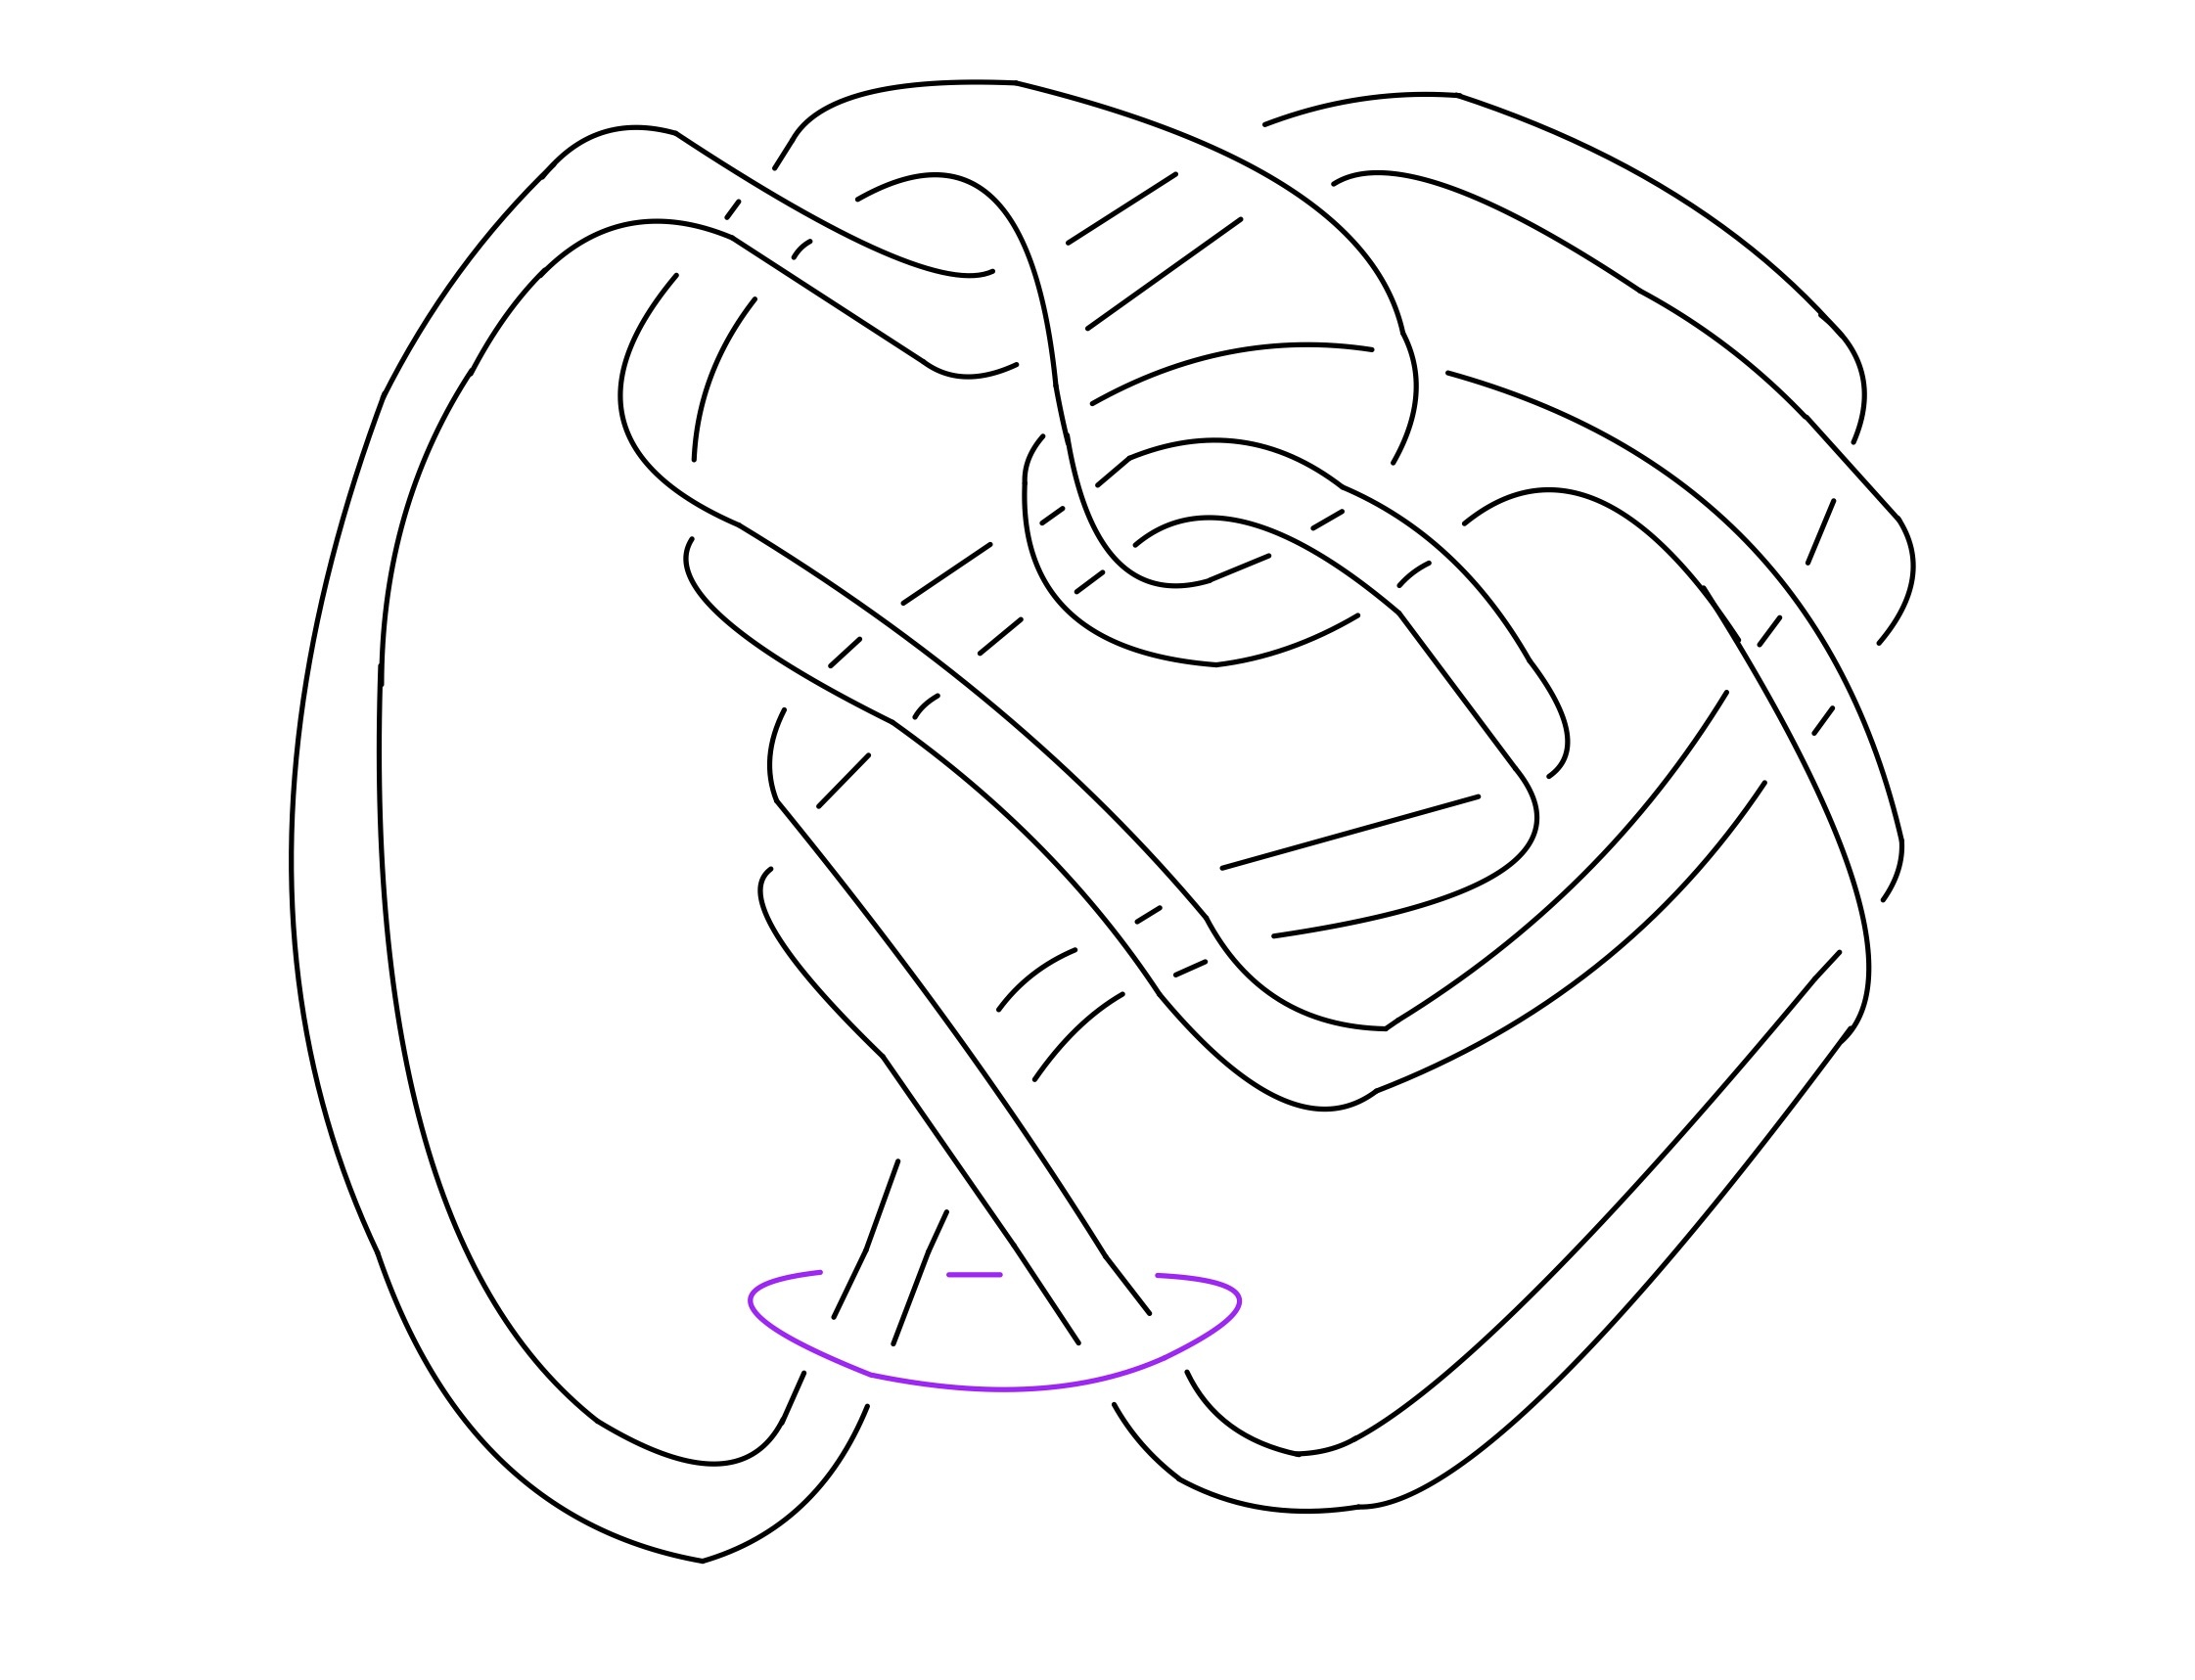
\includegraphics[scale=0.12]{figures/hyper.jpeg}
    \caption{$K_0$ and a curve $\gamma$ in its exterior, used to analyze the hyperbolic structure}
    \label{fig:hyper}
\end{figure}
\begin{defn}
A hyperbolic manifold $M$ is defined to be asymmetric if $$Isom(M) = 1$$.
\end{defn} 
\begin{cla}
$\s^3 \setminus K_0$ and $\s^3 \setminus (K_0 \cup \gamma)$ are asymmetric hyperbolic $3$ manifolds.
\end{cla}
This claim is verified using Snappy, with the computations detailed in the appendix \ref{app}.
It is well known that all hyperbolic manifolds, arising from knot complements, are $1$-cusped \cite{thurston1997geometry}. The following Lemma guarantees that $\s^3 \setminus K_m$ is also a hyperbolic asymmetric $3$ manifold for all but finitely many values of $m < 0$.
\begin{lem} \cite{dhl}\label{cuspi}
Let $M$ be an asymmetric, $1$ - cusped, hyperbolic $3$ manifold. \\
Then all but finitely many Dehn fillings of $M$ are hyperbolic and asymmetric.
\end{lem}
Let $m \leq 0$ be a value satisfying the conditions of the previous Lemma.
As the inclusion of $Isom(M)$ into $Diff(M)$ is a homotopy equivalence for hyperbolic $3$ manifolds $M$ \cite{gabai:smale},  $$
\restr{\varphi}{\s^3 \setminus K_m} \in Diff(\s^3 \setminus K_m)
$$is isotopic\footnote{In this setting, homotopic diffeomorphisms are isotopic by Waldhausen's work \cite{Waldhausen1968}.} to the identity. Restricting this isotopy gives $\restr{\varphi}{U}$ is isotopic to $id_U$.
Finally, we glue the latter with an isotopy of $\restr{\varphi}{V}$ which leaves $\s^3 \setminus \nu(K_m)$ untouched. Hence the thesis.
\endproof
Consider $\restr{\varphi}{\s^3}$. By the previous Lemma , we can assume, up to isotopy, that $$
\restr{\varphi}{\s^3 \setminus \inter} = id_{\s^3 \setminus \inter}
$$
Then we can extend the isotopy to the whole $\B^4$, requiring that it is supported away from $D$. \\
Our strategy involves finding a knot $J \subseteq \s^3 \setminus K$ that bounds a disk in $\B^4 \setminus D'$ but not in $\B^4 \setminus D$.
Consider the green curve $J$ drawn in figure \ref{fig:km}. \\
\begin{cla}$J$ bounds an embedded disk $\mathfrak{D}'$, which is disjoint from $D'$.
\end{cla}
We analyze $J$ within the Kirby diagram of $\B^4 \setminus \interd$ as in figure \ref{fig:comp21} (a) and (b). Since $J$ does not pass through the $1$-handles, it bounds a disk embedded in $\estdi$, which is tautologically disjoint from $D'$.
\\ \\ 
As $\varphi$ fixes $\s^3 \setminus \inter$, in particular, $J$ is fixed. \\
Thus $$
\varphi(\mathfrak{D}') = \mathfrak{D} 
$$is a disk with $$
\partial \mathfrak{D} = J
$$
Moreover, it is disjoint from $D$, otherwise $\varphi^{-1}(\mathfrak{D}\cap D) = \mathfrak{D'} \cap D' \neq \emptyset$, that is not possible due to construction. 
\section{Double Branched Cover Argument} \label{buffet}
We employ the double branched cover construction to obstruct the existence of $\mathfrak{D}$. \\ \\ We build $\Sigma(\B^4, D)$ following the instructions from section \ref{covers}. 
In order to draw a Kirby diagram for $\Sigma(\B^4, D)$, we use the following strategy which is divided into three steps. \\ \\
\textbf{Step 1}: Draw a Kirby for the disk exterior (It is depicted in Figure \ref{fig:comp1}(a)-(f)).\\ \\
\textbf{Step 2}: By examining the $\Z/2\Z$ action on $1$-handles, draw a Kirby diagram for the double covering of $\estd$. \\ \\
\textbf{Step 3}: Fill the branch locus by adding a $2$-handle, that will cancel itself together with a $1$-handle. \\ \\
 First, we describe a Kirby diagram for the double covering of $\estd$. Let $\varphi: \pi_1(\estd) \rightarrow \Z/2\Z$ be the surjective map which defines such covering. 
Consider Figure \ref{fig:comp1}(f). Recall that $\pi_1(\estd)$ is generated by $y$, that is the core curve of the upper $1$-handle $H_1$. Thus $\varphi(y) = 1$. Since we performed a handle slide in step (c) of Figure \ref{fig:comp1}, the core curve of the other $1$-handle, lies in $2\Z = Ker(\varphi)$. \\ Observe that $\B^4 \cup H_1 \cong \s^1 \times \B^3$ is double covered by $\s^1 \times \B^3$ via the map $(e^{it}, x) \rightarrow (e^{2it}, x)$. Therefore, $H_1$ lifts to a single $1$-handle. On the other hand, each of the remaining handles lift to two copies of them. 
\begin{note} A bare hand computation (via the double strand notation), shows that the $2$-handle framings are preserved on each lifted copy.
\end{note}
So we need to juxtapose two copies of Figure \ref{fig:branch1}(a), as suggested on the right side. Figure \ref{fig:branch1}(b) depicts the Kirby diagram of the double covering of $\B^4 \setminus D$. Finally, we fill the branch locus $D$, by removing a $1$-handle as in Figure (c). That is the Kirby diagram of $\Sigma(\B^4, D)$. Notice that the simmetry makes the $\Z/2\Z$ action evident. \\ \\
Next, we simplify the diagram. In step (d), we slide a $2$-handle over the other. In Figure \ref{fig:branch3}(f) we add a curl. Then in step (g) we perform a $2$-handle slide again (we report only a local picture). In Figure \ref{fig:branch4}(h) we cancel the handle pair. The other steps (i)-(n) are just isotopies. Throughout this process, we track the green curve $\tilde{J}$, an arbitrary lift of $J$.
\begin{figure}[H]
    \centering
    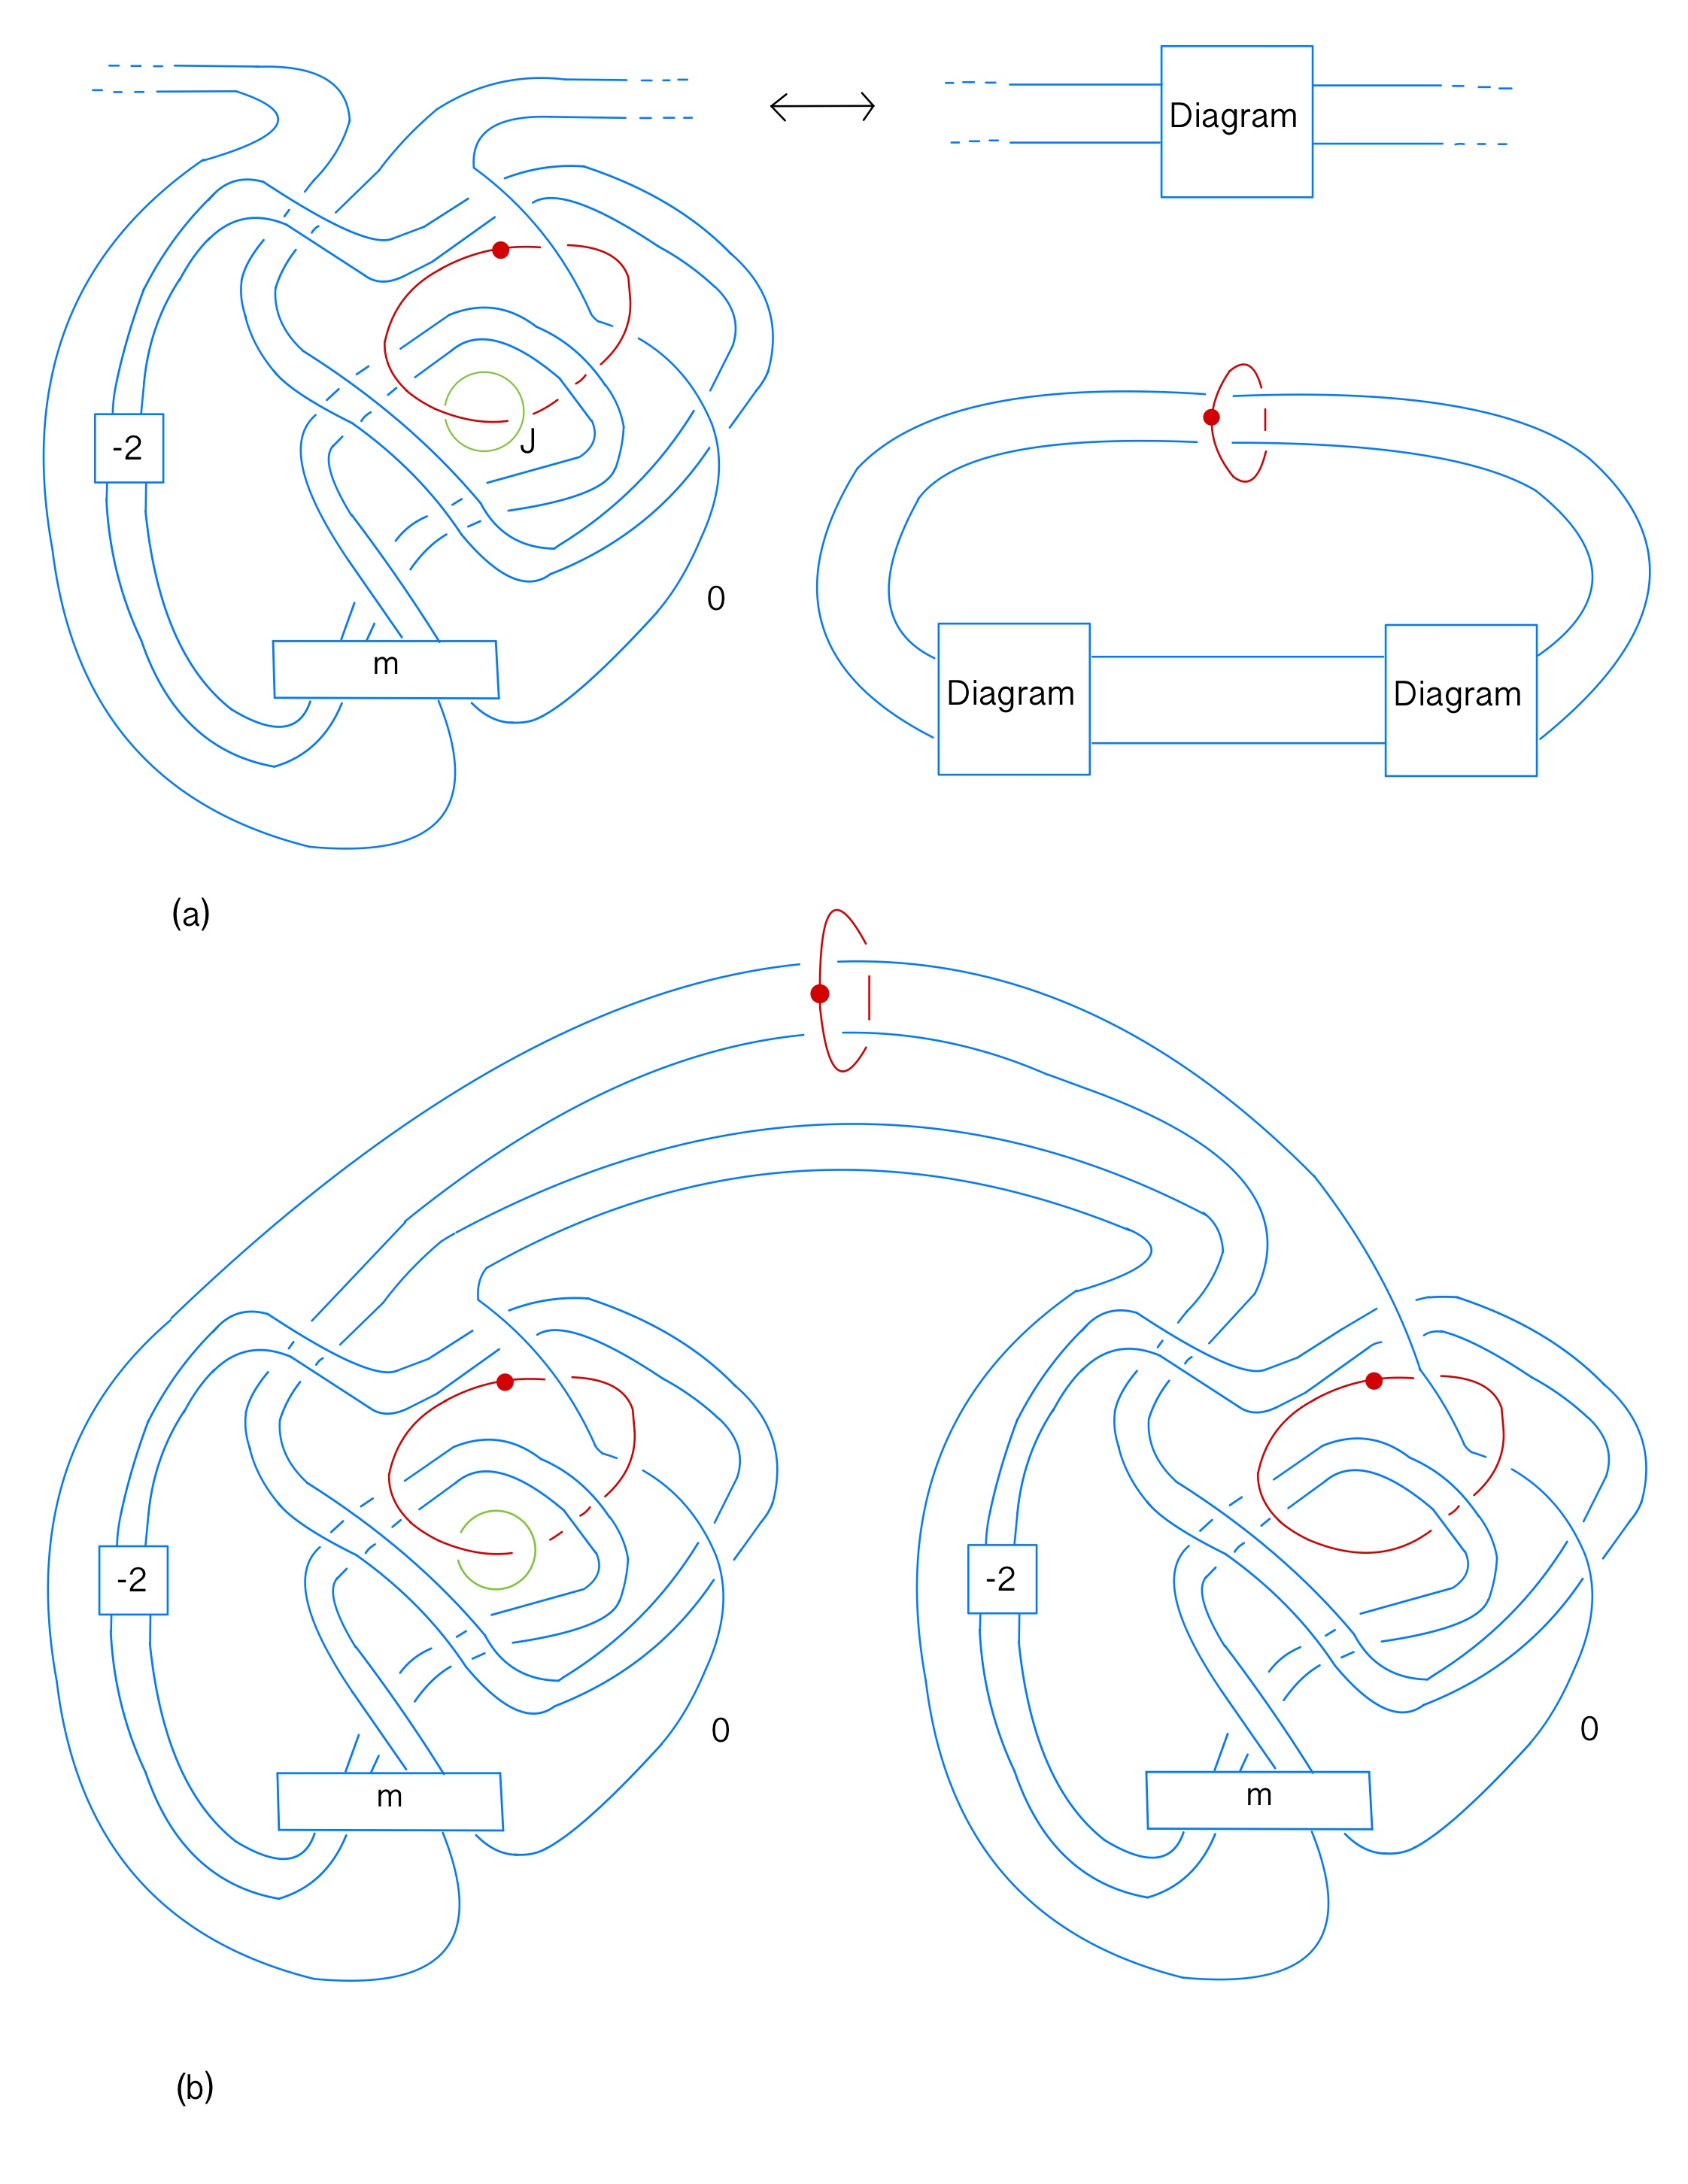
\includegraphics[scale=0.2]{figures/branch1.jpeg}
    \caption{Construction of the double branched covering, with the branch locus removed}
    \label{fig:branch1}
\end{figure}
\begin{figure}[H]
    \centering
    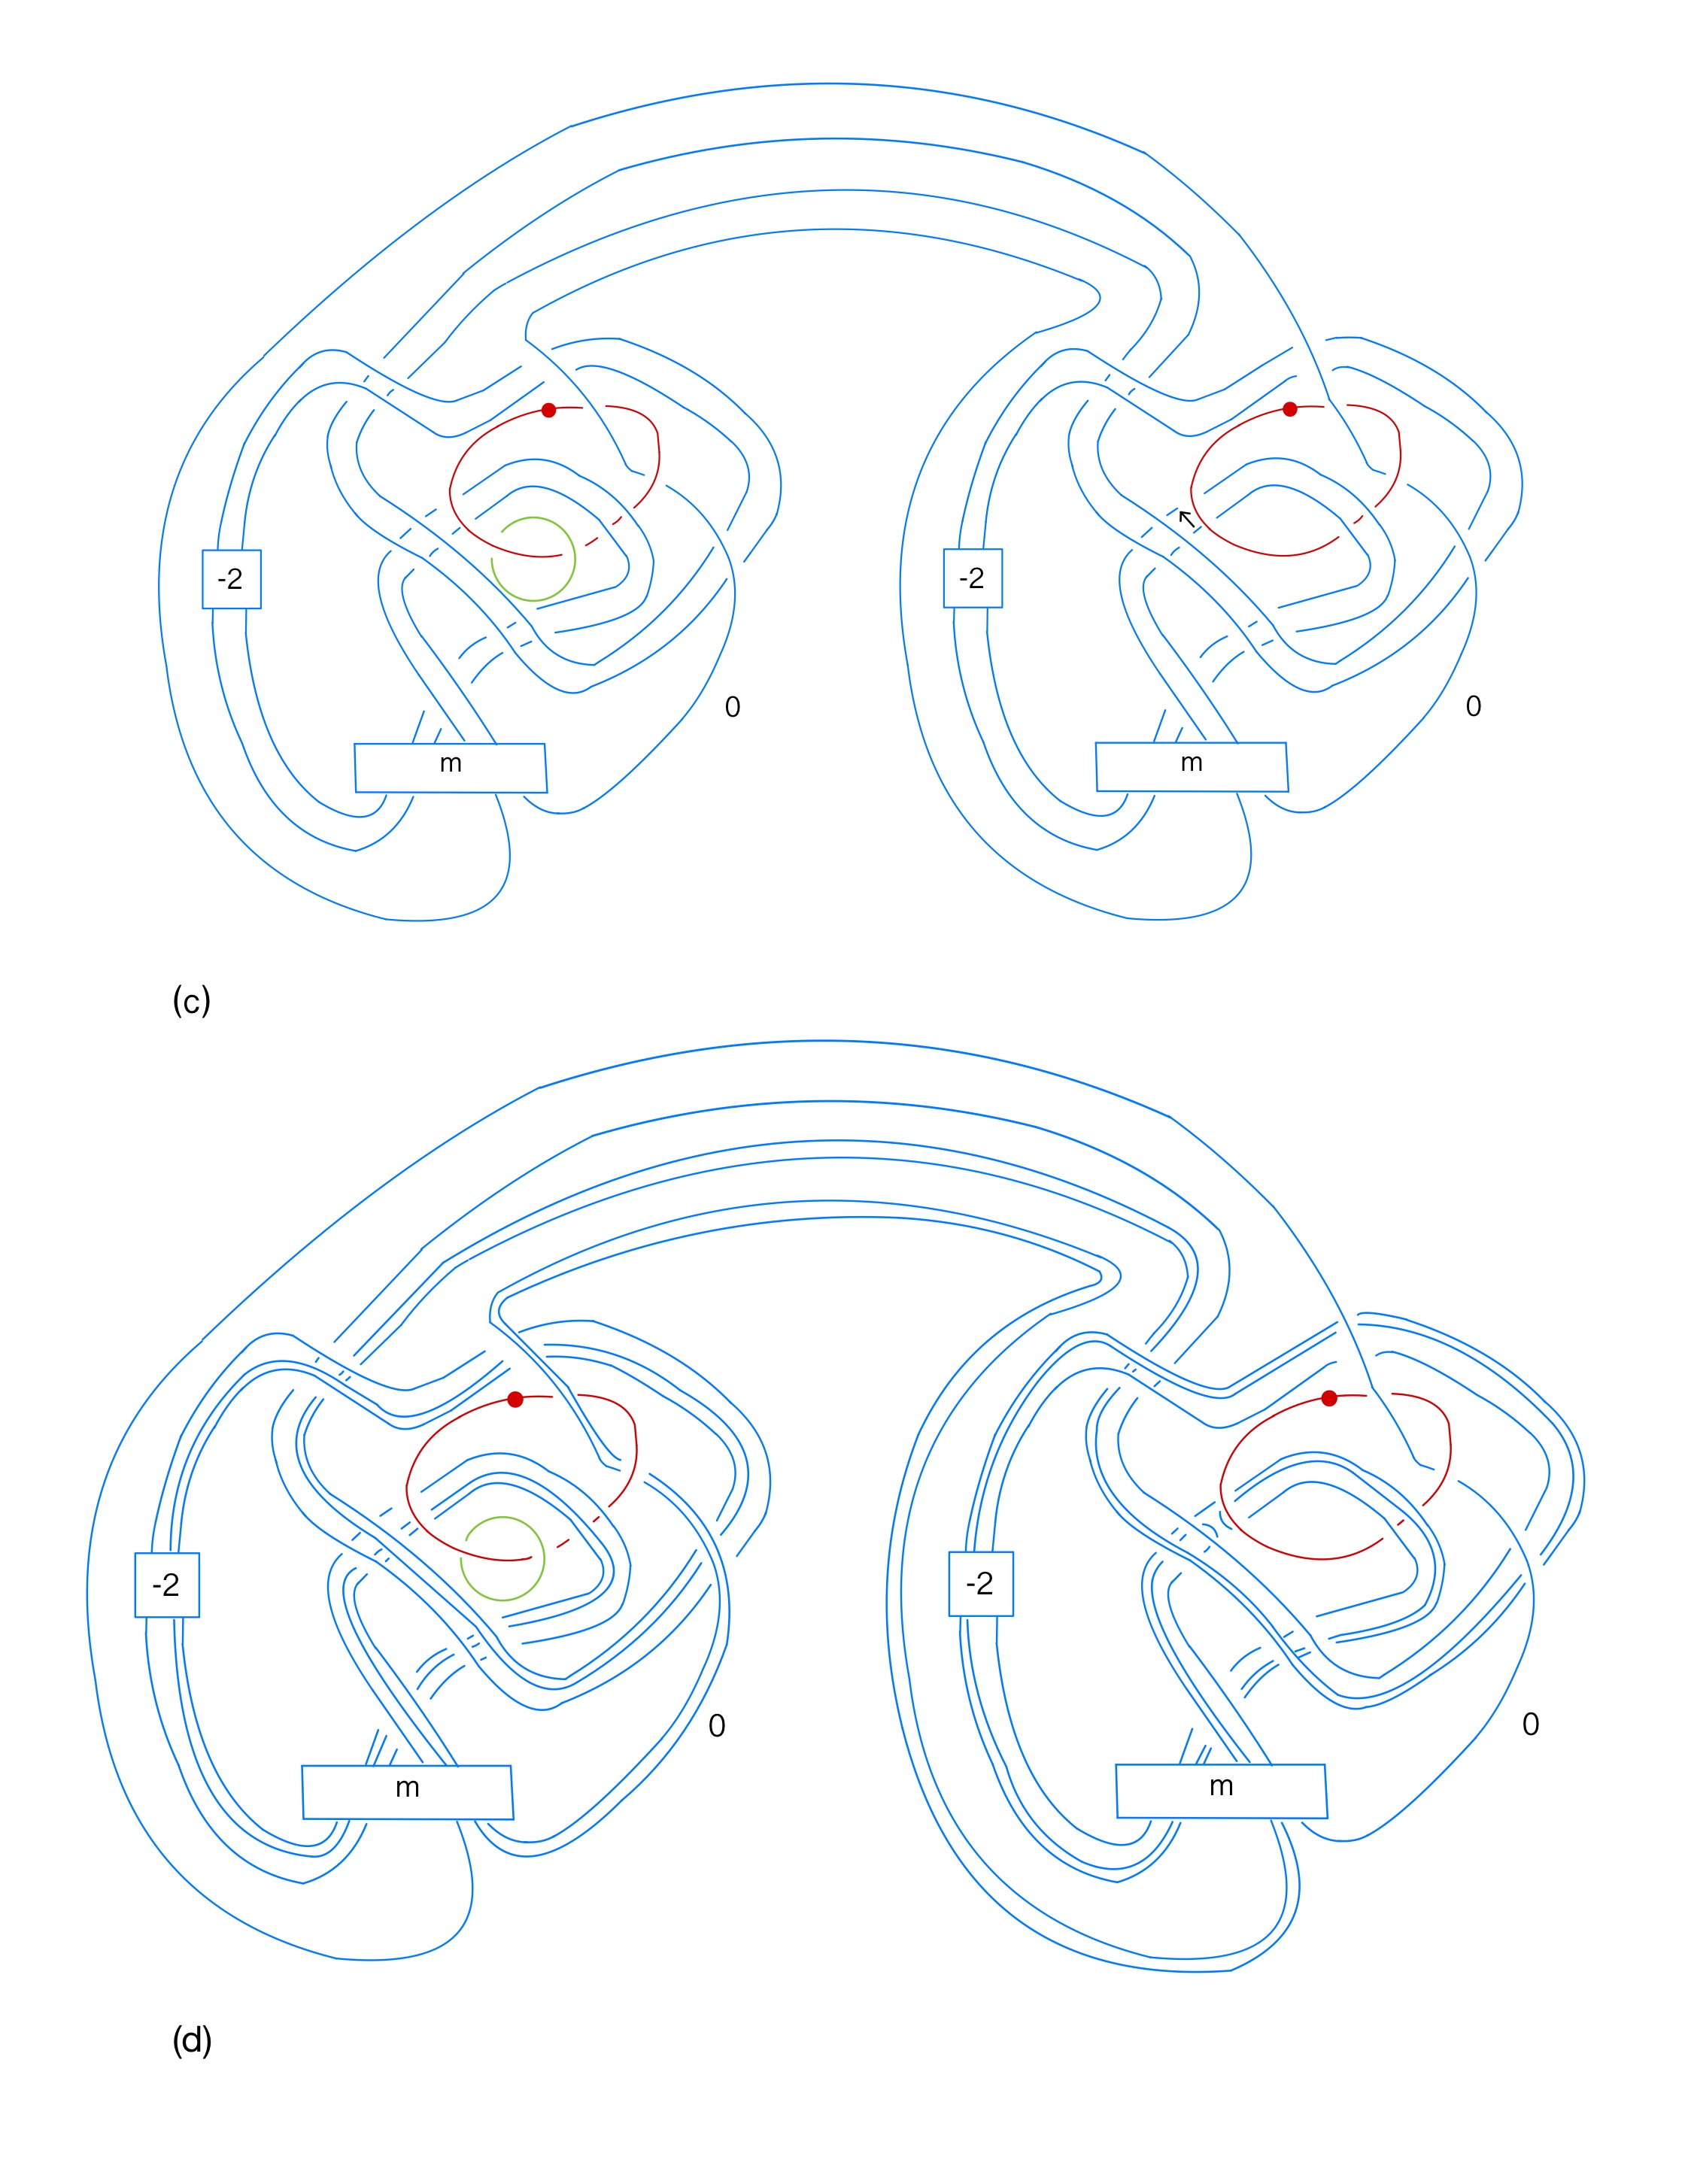
\includegraphics[scale=0.2]{figures/branch2.jpeg}
    \caption{The Kirby diagram of the double branched covering on top}
    \label{fig:branch2}
\end{figure}
\begin{figure}[H]
    \centering
    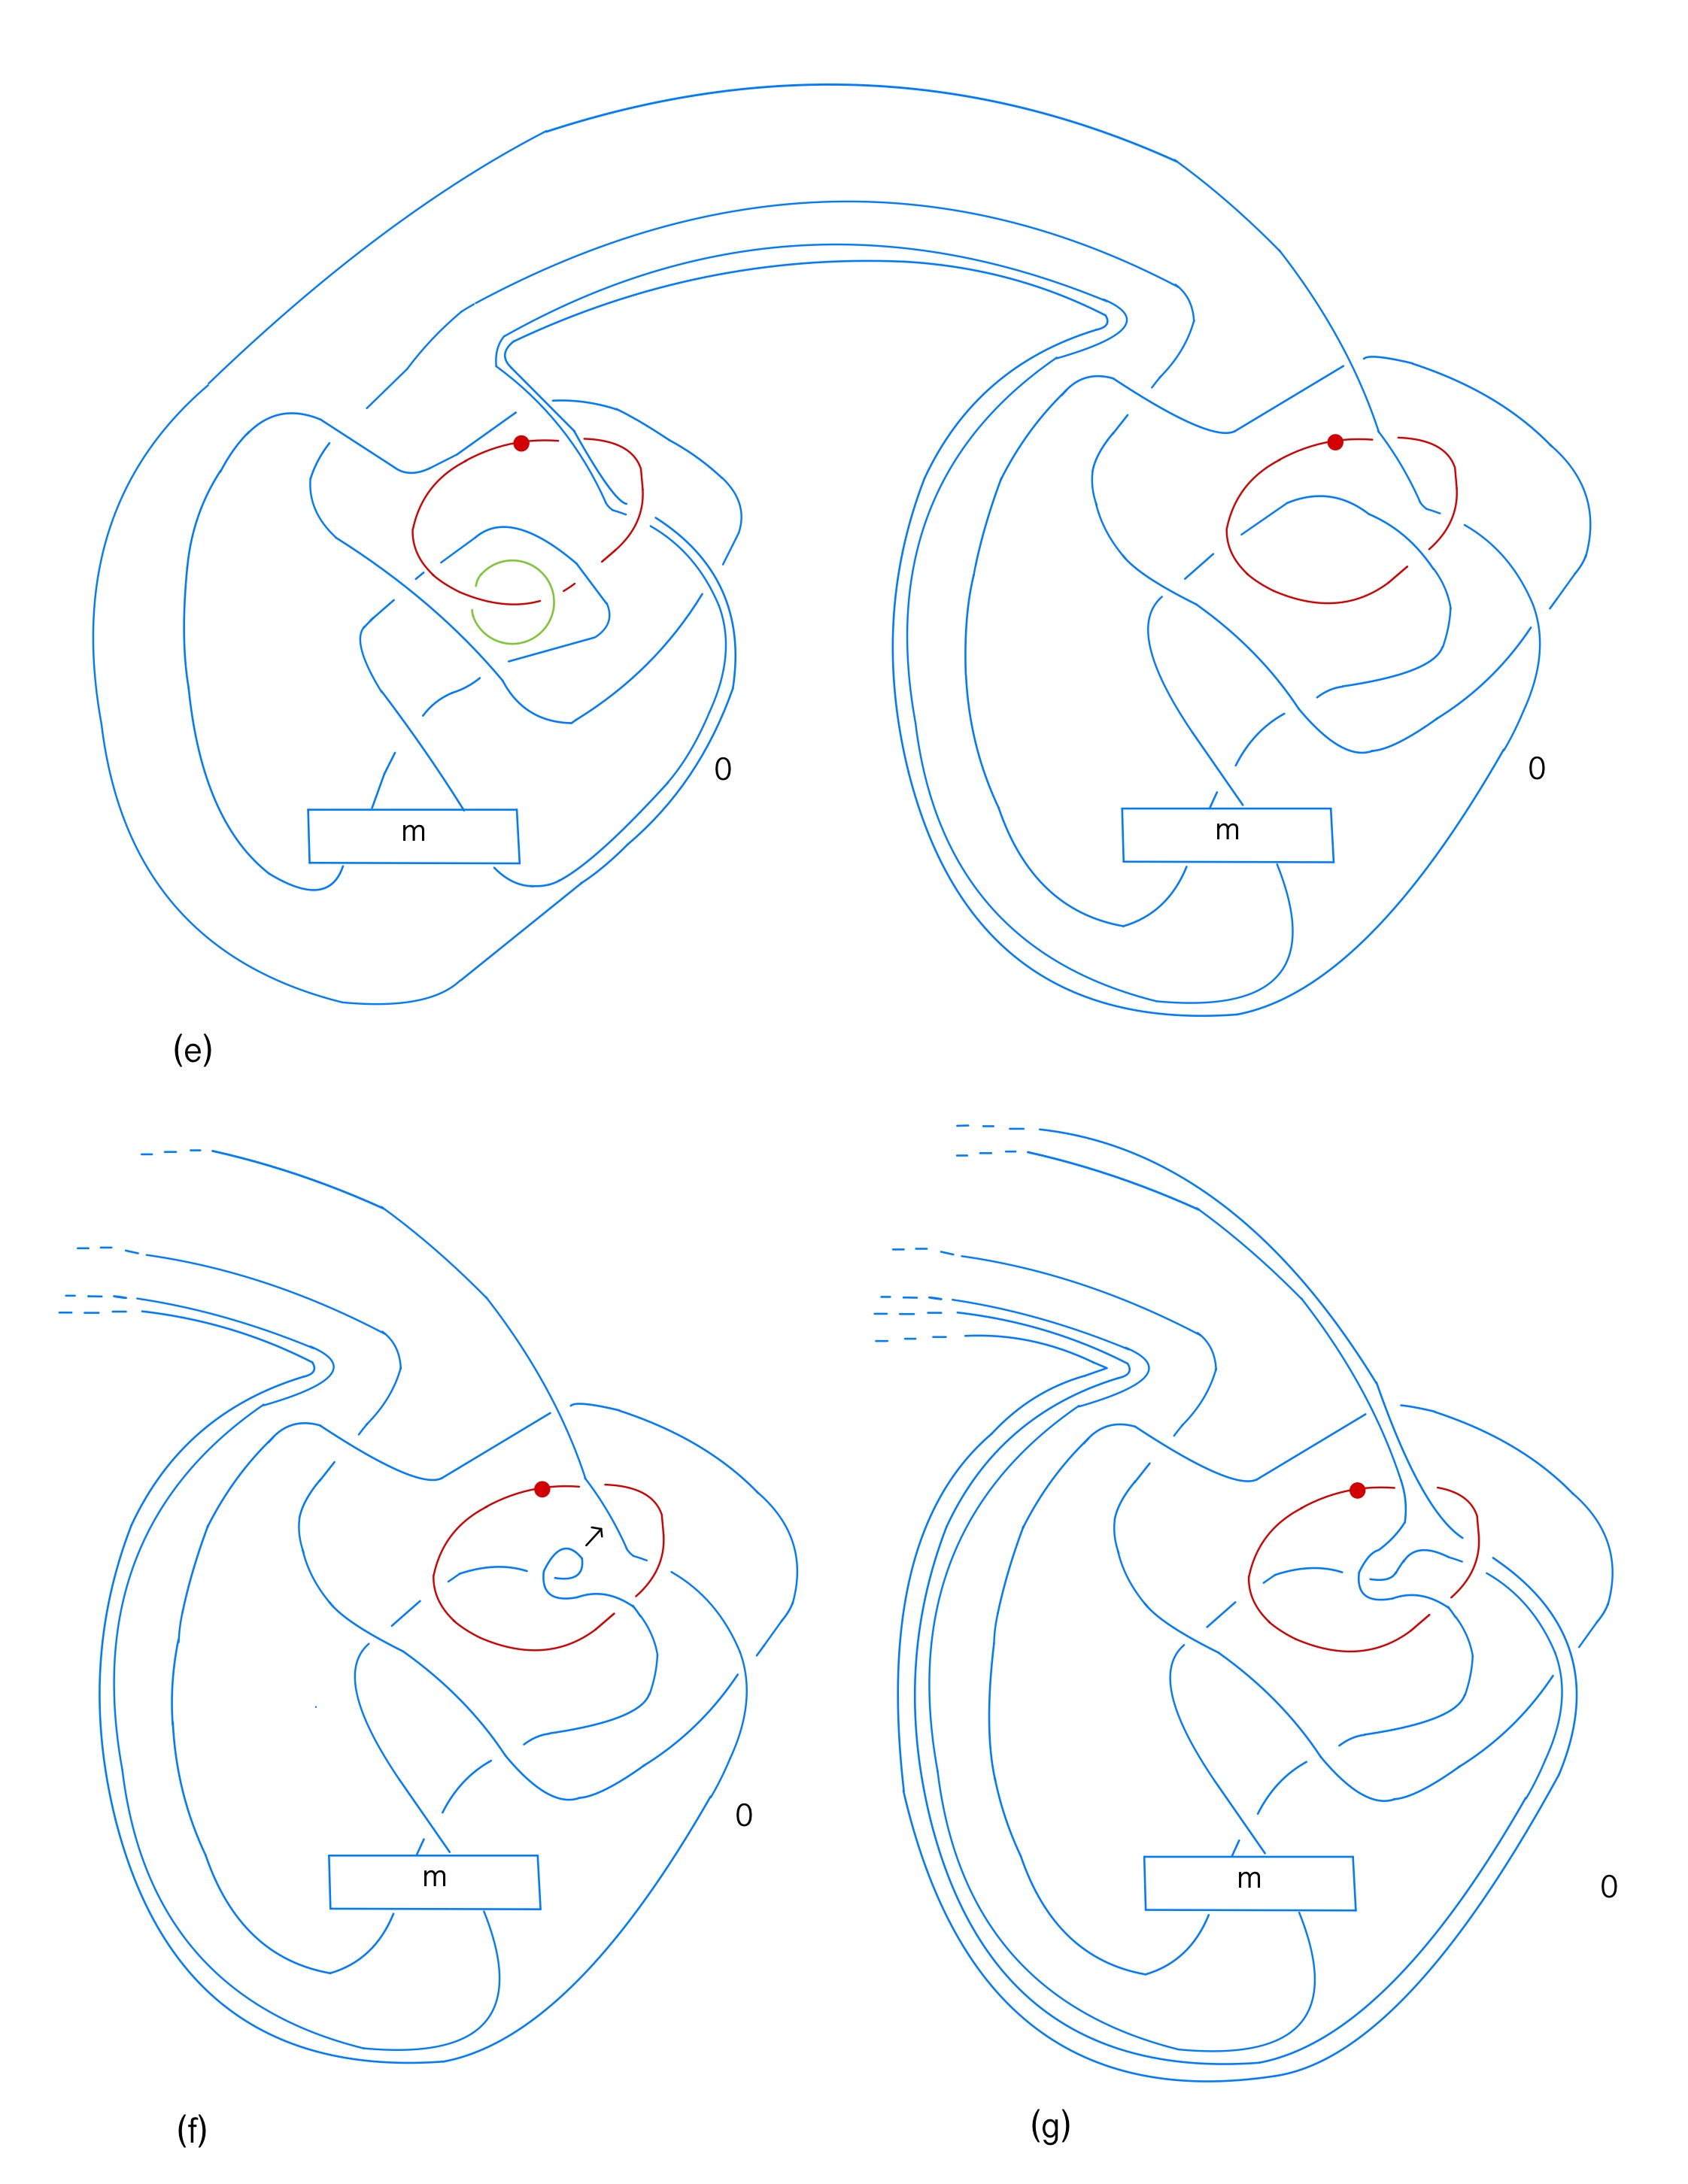
\includegraphics[scale=0.2]{figures/branch3.jpeg}
    \caption{Handle slide and isotopies}
    \label{fig:branch3}
\end{figure}
\begin{figure}[H]
    \centering
    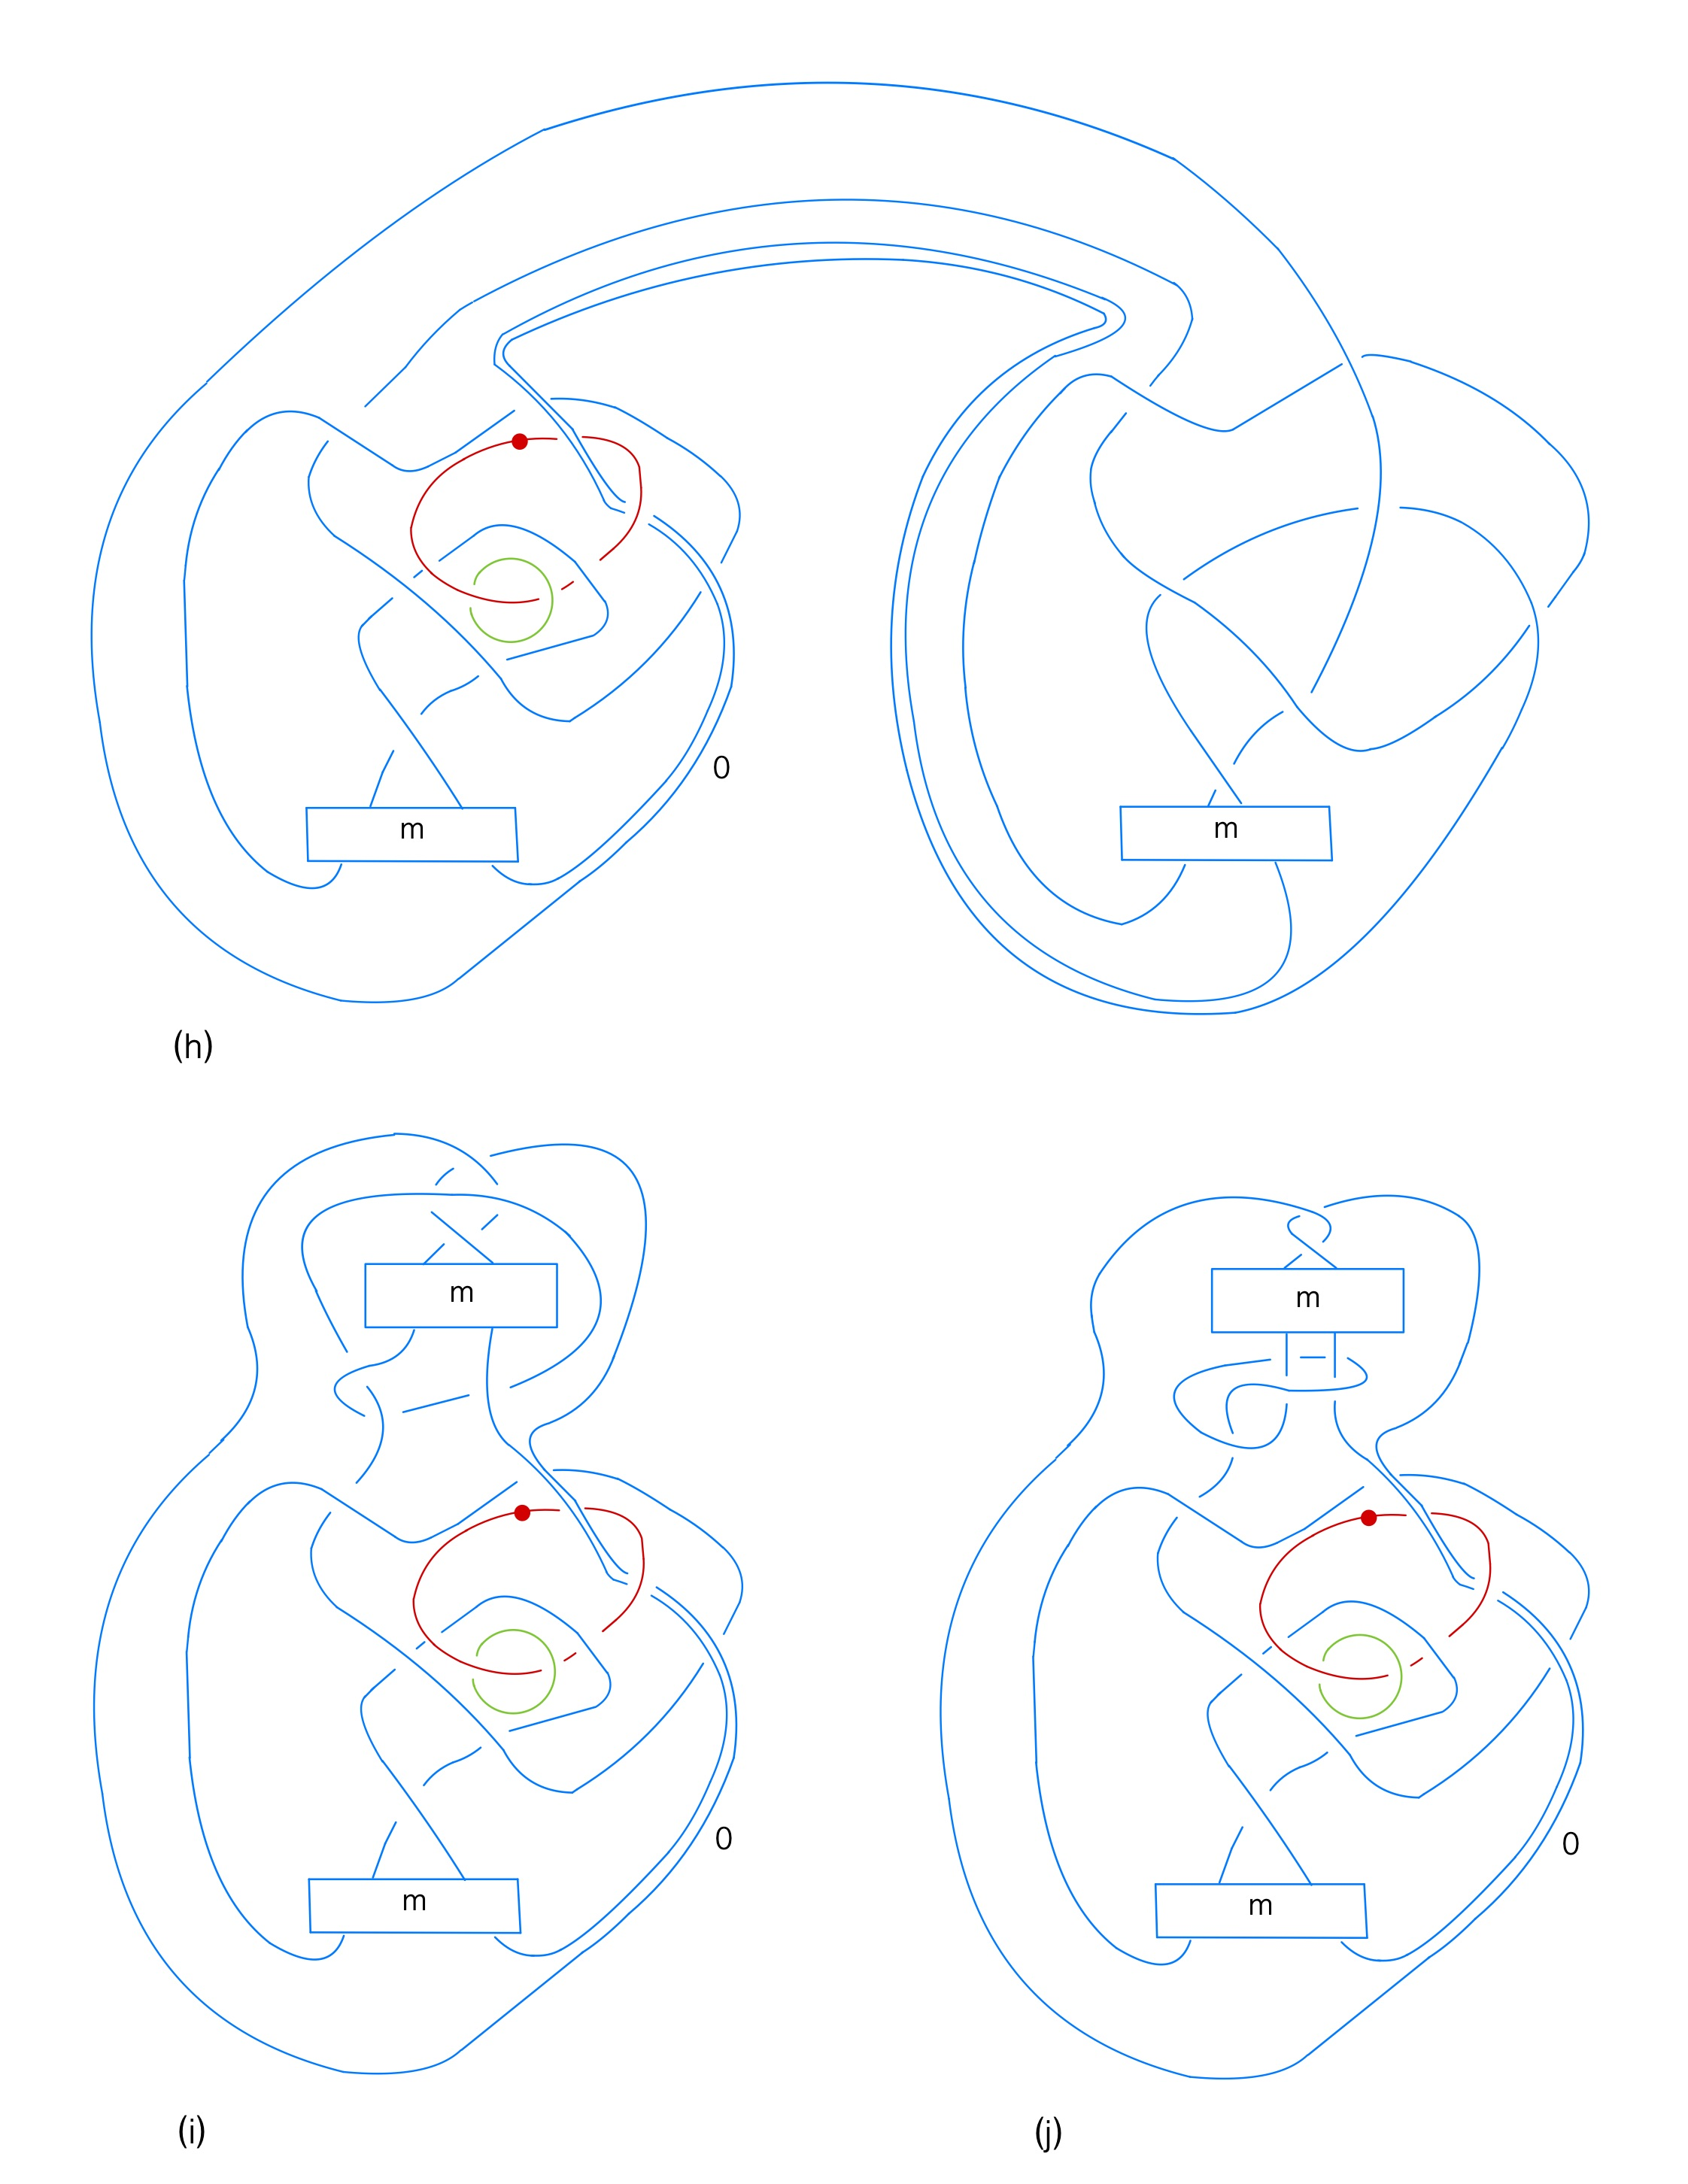
\includegraphics[scale=0.2]{figures/branch4.jpeg}
    \caption{Handle cancellation and isotopies}
    \label{fig:branch4}
\end{figure}
\begin{figure}[H]
    \centering
    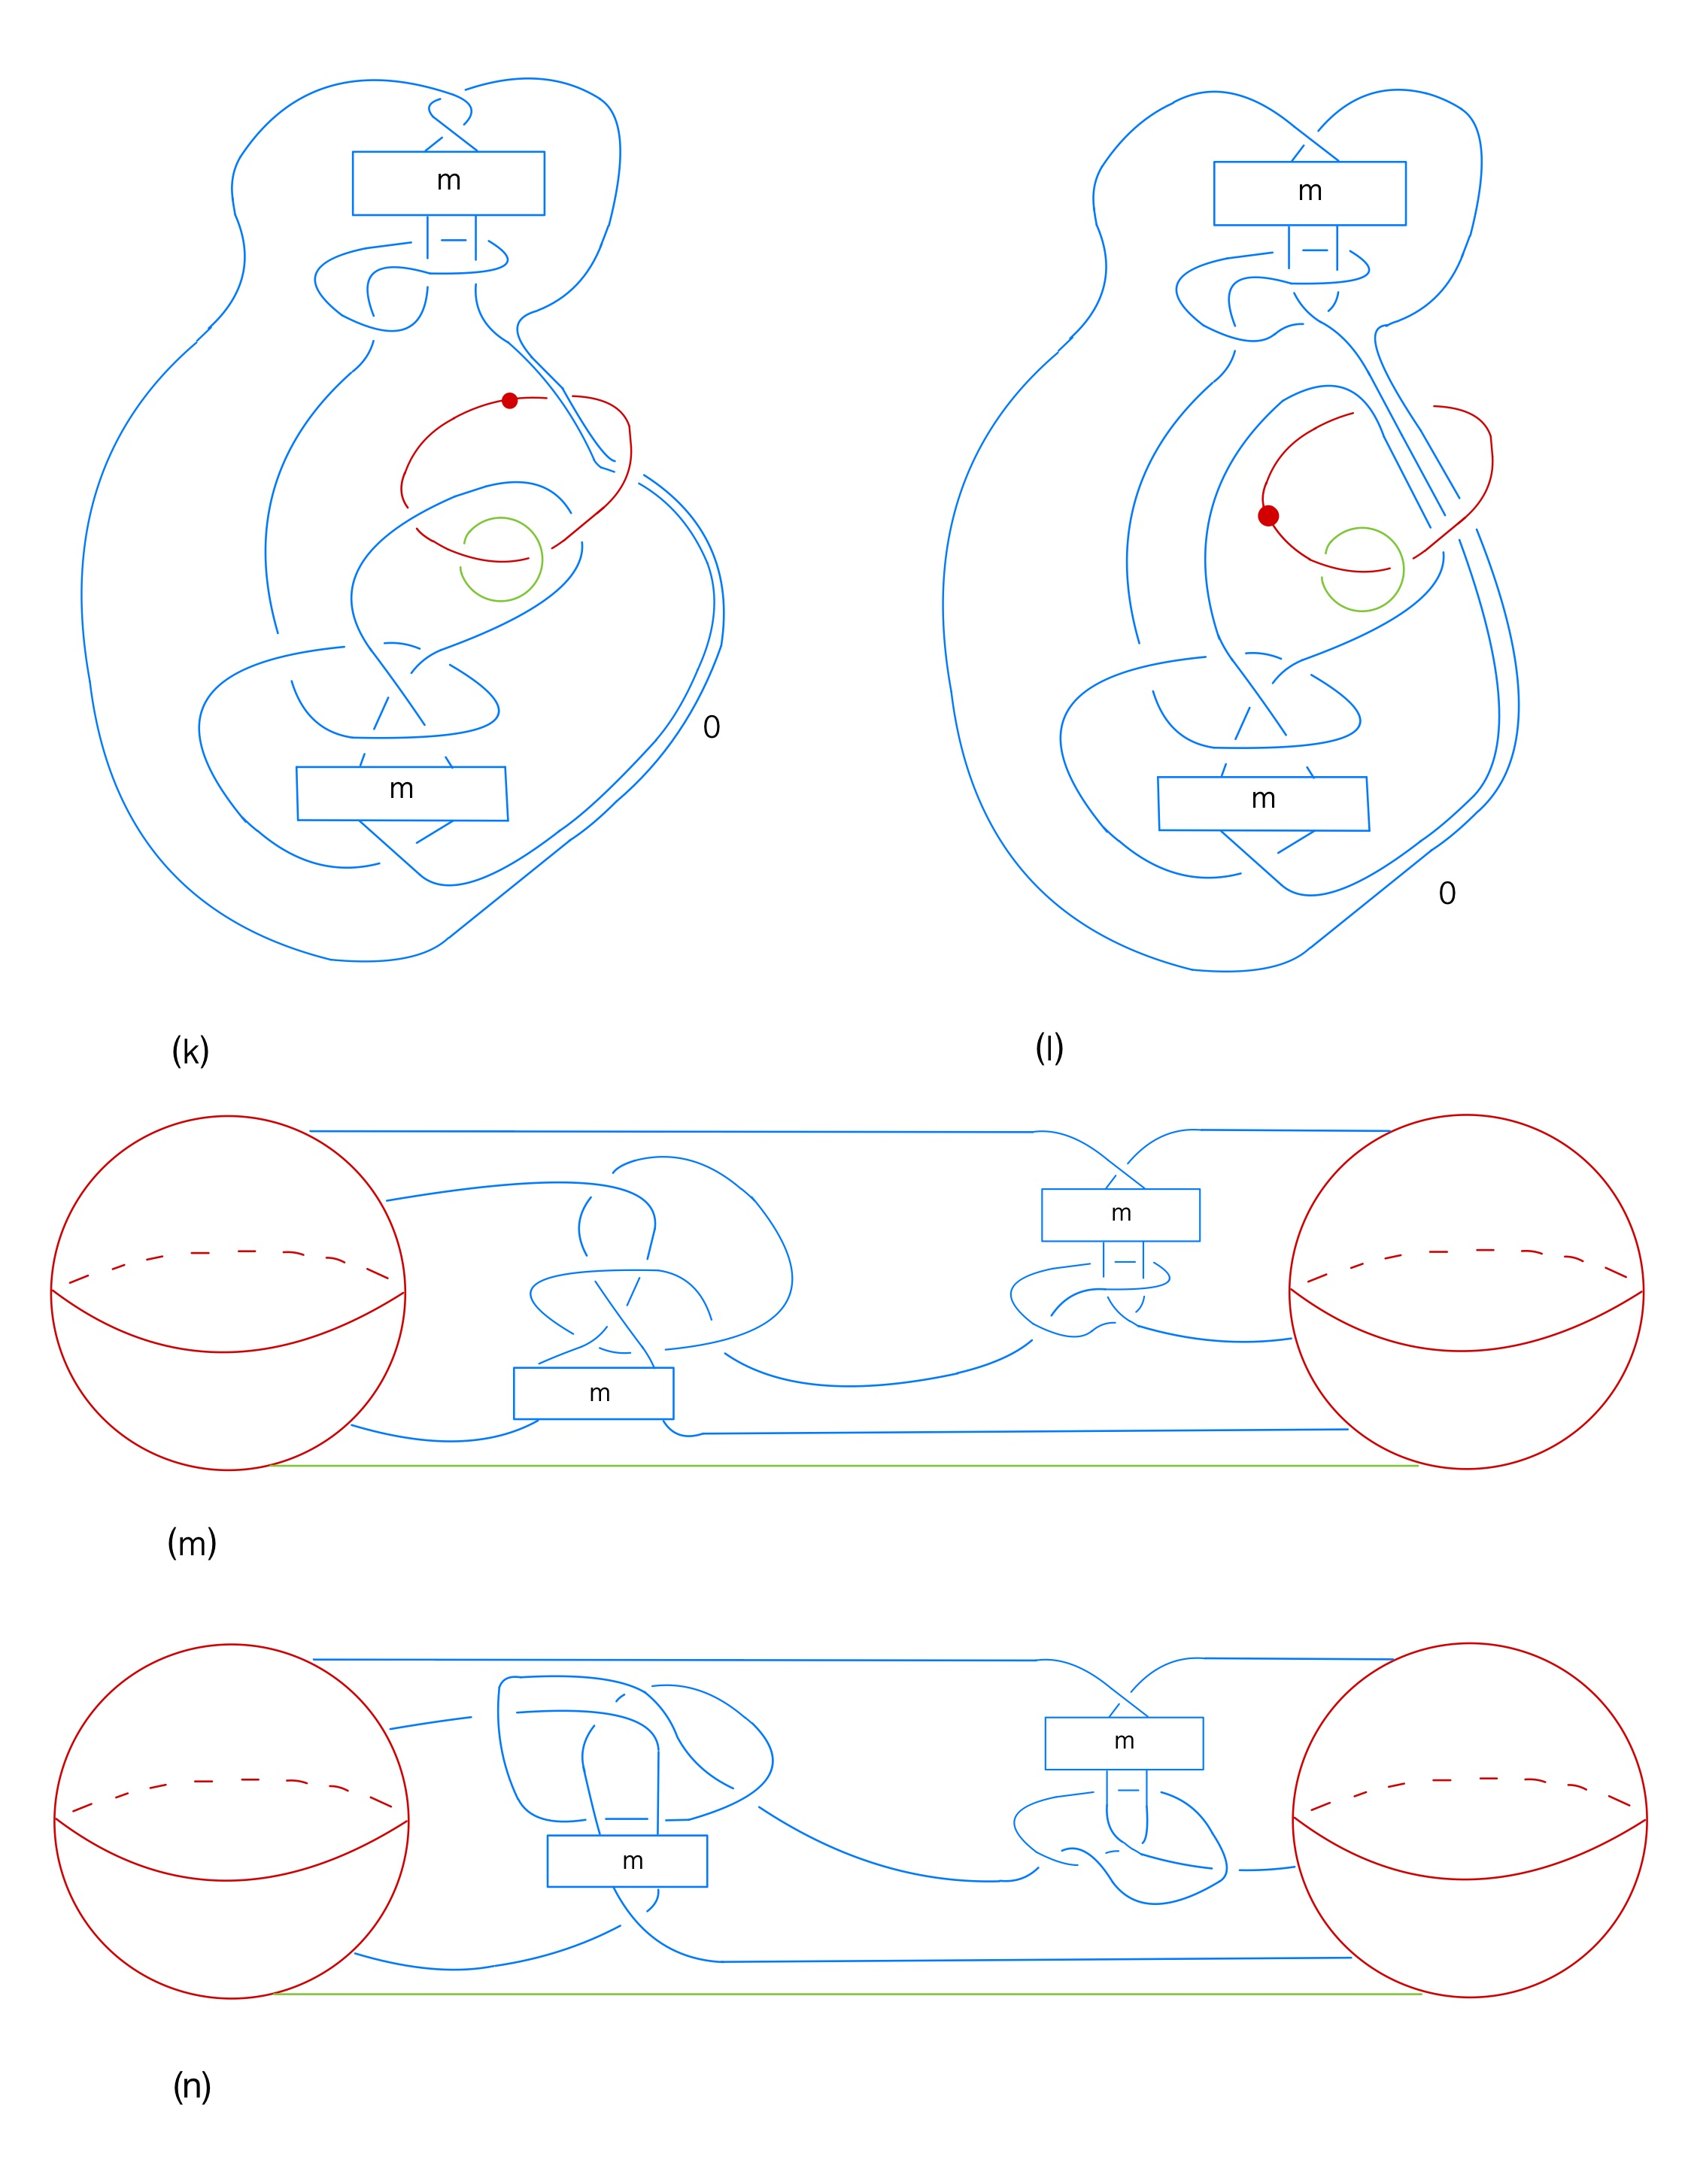
\includegraphics[scale=0.2]{figures/branch5.jpeg}
    \caption{A sequence of isotopies}
    \label{fig:branch5}
\end{figure}
\section{The Evocation of Stein Structures}\label{summon}
We now aim to equip $W$ with a Stein structure. 
We realize the $2$- handle of figure \ref{fig:branch5} as a Legendrian tangle. Thus, we obtain a diagram in Gompf's standard form (discussed in section \ref{gom}).
\begin{figure}[H]
    \centering
    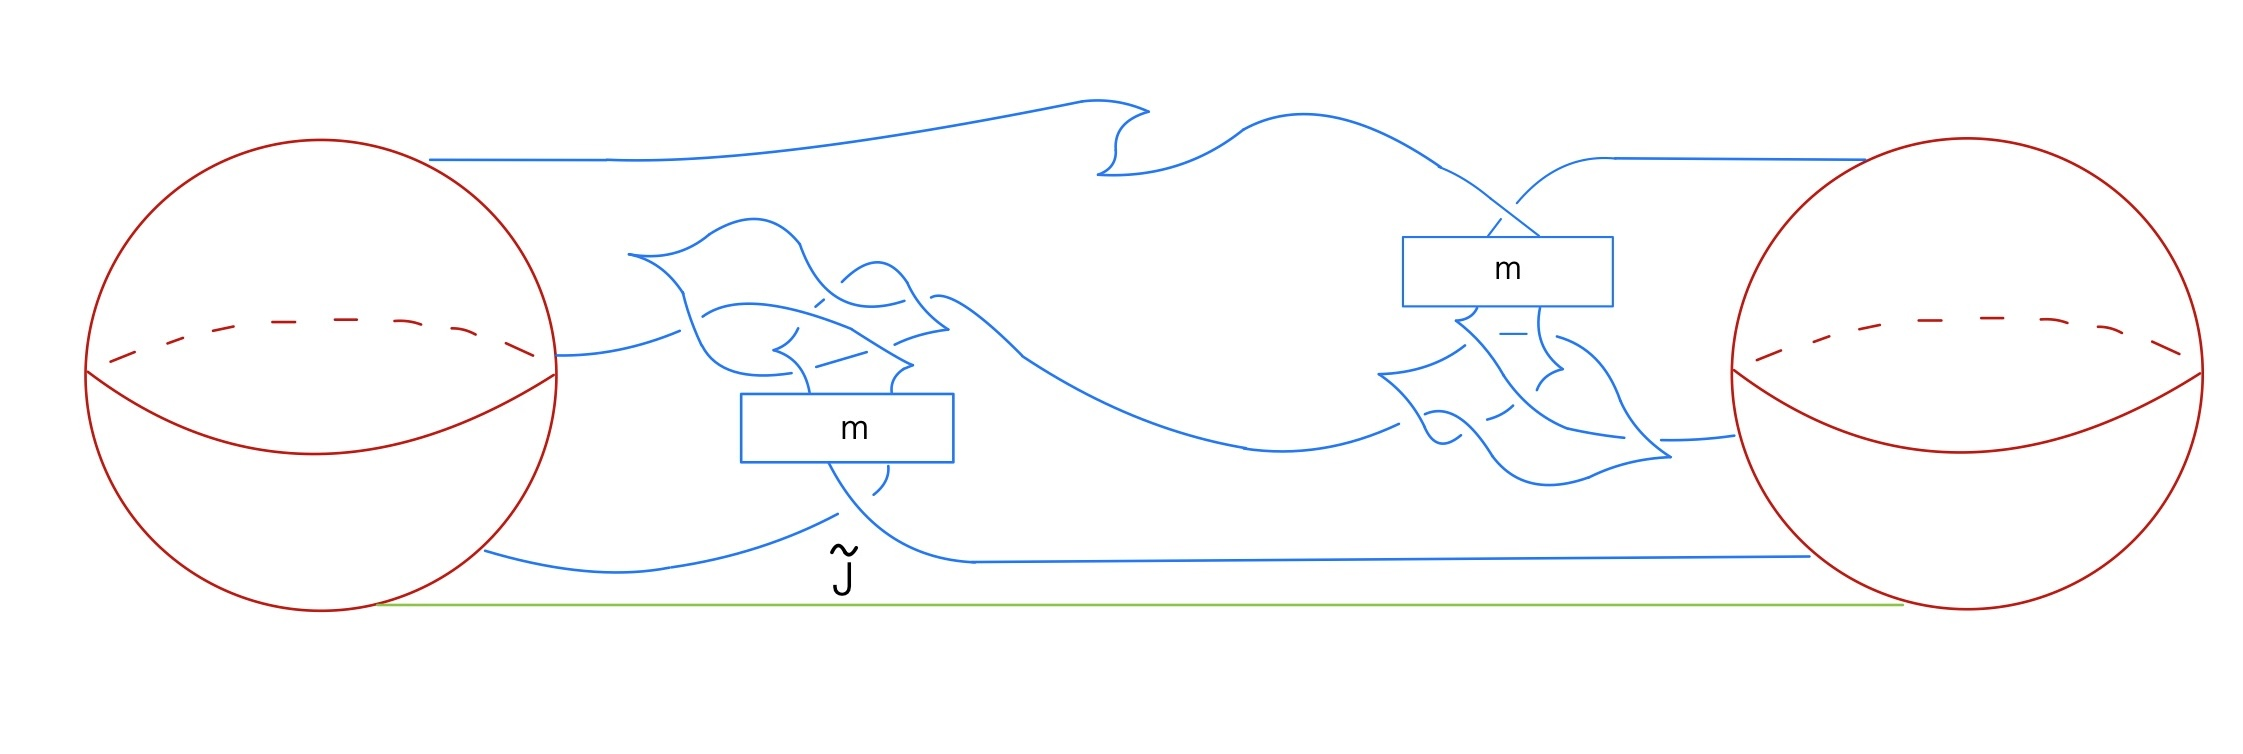
\includegraphics[scale=0.2]{figures/tb.jpeg}
    \caption{The Kirby diagram of $\Sigma(\B^4, D)$ presented in Gompf's standard form}
    \label{fig:tb}
\end{figure}
\begin{rem}
The formula $$
tb(K) = w(K) - \#\{\text{right cusps} \}
$$holds in Gompf's standard form. 
\end{rem}
This allows us to compute the Thurston - Bennequin number directly from \ref{fig:tb}.
We have: $$
tb(\mathfrak{k}) - 1 = 2m+6 - (2m+5) - 1 =  0 
$$
where $\mathfrak{k}$ is the Legendrian curve representing the $2$-handle.
We invoke Eliashberg's characterization theorem \ref{el}, to equip $W$ with Stein structure.
We attach a $2$ - handle $H_2$ along $\tilde{J}$ with framing $-1$. 
Since $\tilde{J}$ has a Legendrian representative without crossings and without cusps, we get$$
tb(\tilde{J}) - 1 = -1
$$
Again, by Eliashberg's theorem, $W' = W \cup H_2$ carries a Stein structure.
Let $\tilde{\mathfrak{D}} \subseteq W$ be a lifting of $\mathfrak{D}$. \\
Inside $W'$, the core of $2$-handle completes $\tilde{\mathfrak{D}}$ to a sphere $S$.
\begin{as}The self intersection of $S$ is $$
S \cdot S = -1
$$
\end{as}
\proof To compute the self intersection, consider a parallel copy of $S$, obtained by pushing it transversely, as in Figure \ref{fig:stein}. Since $tb(\partial \tilde{\mathfrak{D}}) = tb(\tilde{J}) =0$, the contribution of $\tilde{\mathfrak{D}}$ is $0$. Moreover, the self intersection of the core of the $2$-handle equals its framing, that is $-1$.
\begin{figure}[H]
    \centering
    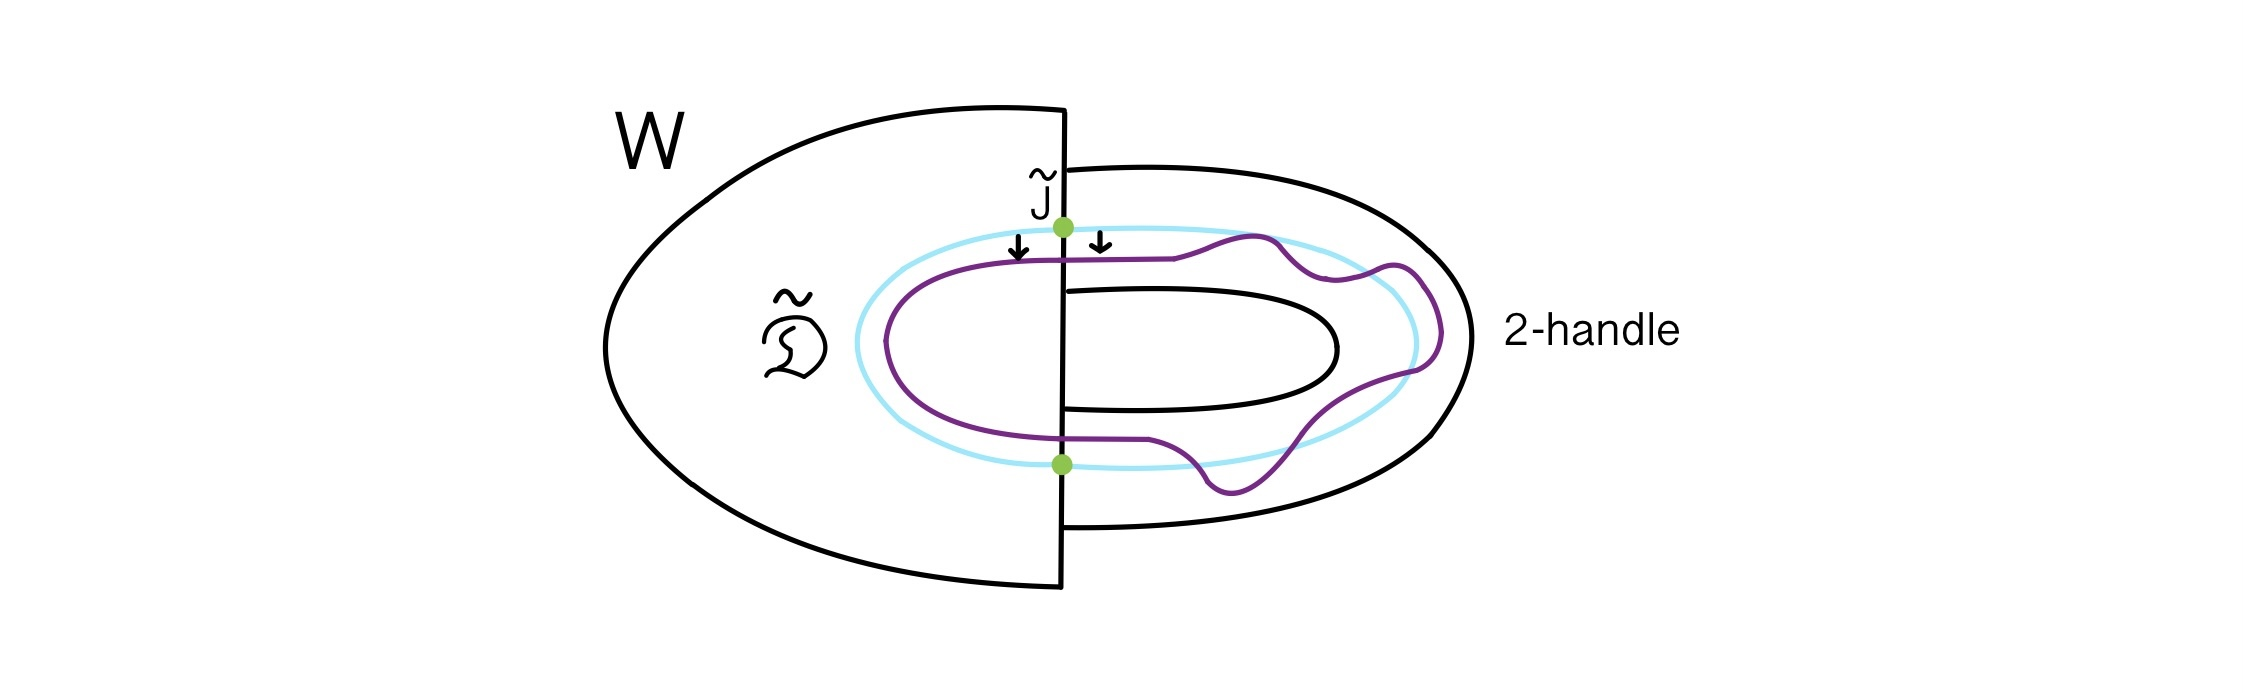
\includegraphics[scale=0.2]{figures/stein.jpeg}
    \caption{Self intersection of the sphere $S$}
    \label{fig:stein}
\end{figure}
\endproof
Proposition \ref{ostruzione} rules out the existence of $S$, thus $J$ cannot bound an embedded disk disjoint from $D$, resulting in the desired contradiction.
This completes the proof of theorem \ref{prince}. \\ \\
In the last chapter, we extend the discussion to the higher genus case.
The following corollary follows naturally from our earlier argument.
\begin{cor}\label{giotto}There exist pairs of exotic, contractible, Stein $4$-manifolds.
\end{cor}
\proof
Set $$
W_1 = \Sigma(\B^4, D) \qquad W_2 = \Sigma(\B^4, D')
$$
Notice that $W_1$ and $W_2$ have the same boundary \footnote{The restriction of a branched covering to the boundary remains a branched covering}, which is $$
\Sigma(\s^3, \partial D) = \Sigma(\s^3,\partial D') = \Sigma(\s^3, K_m)
$$
Since $D$ and $D'$ are topologically isotopic, then $W_1$ and $W_2$ are homeomorphic.
Assume by contradiction there exist a diffeomorphism $\psi : W_2 \rightarrow W_1$, that restricts to the identity on the boundary $\Sigma(\s^3, K_m)$.
Let $\tilde{\mathfrak{D'}} \subseteq W_2$ be a lifting of $\mathfrak{D'}$. Then $\psi(\tilde{\mathfrak{D'}})$ is a disk embedded in $W_1$, which is bounded by $\psi(\tilde{J}) = \tilde{J}$. Using the argument above, this leads to a contradiction. 
\endproof
\section{Theoretical Road}
Although Theorem \ref{prince} has been proven, we will also demonstrate that the disks arising from Figure \ref{fig:trecolori} are exotic. This demonstration is significant because it proves exoticness directly from the initial diagrams (the non-standard diagrams of $\B^4$). The advantage is that we can avoid finding the explicit band structure of the disks.
This has two additional purposes: 
\begin{itemize}
    \item Explain a straightforward way to find a Kirby diagram for the disk exterior,
    \item Enlight a lucky shortcut in the final argument.
\end{itemize}
We mimic the previous proof. First of all, we estabilish the topological isotopy, following \cite{hayden2023brunnianexoticsurfacelinks}. To that end, we draw Kirby diagrams for the disks exteriors.  
Carving an unknotted disk equals to add a $1$-handle. Thus it suffices to put a dot on $K$ on both diagrams \ref{fig:trecolori}(a), (b). We get Figures \ref{fig:shortcut1}(a) \ref{fig:shortcut2}(a). Then we isotope the two dotted circles to a two component unlink.
\begin{figure}[H]
    \centering
    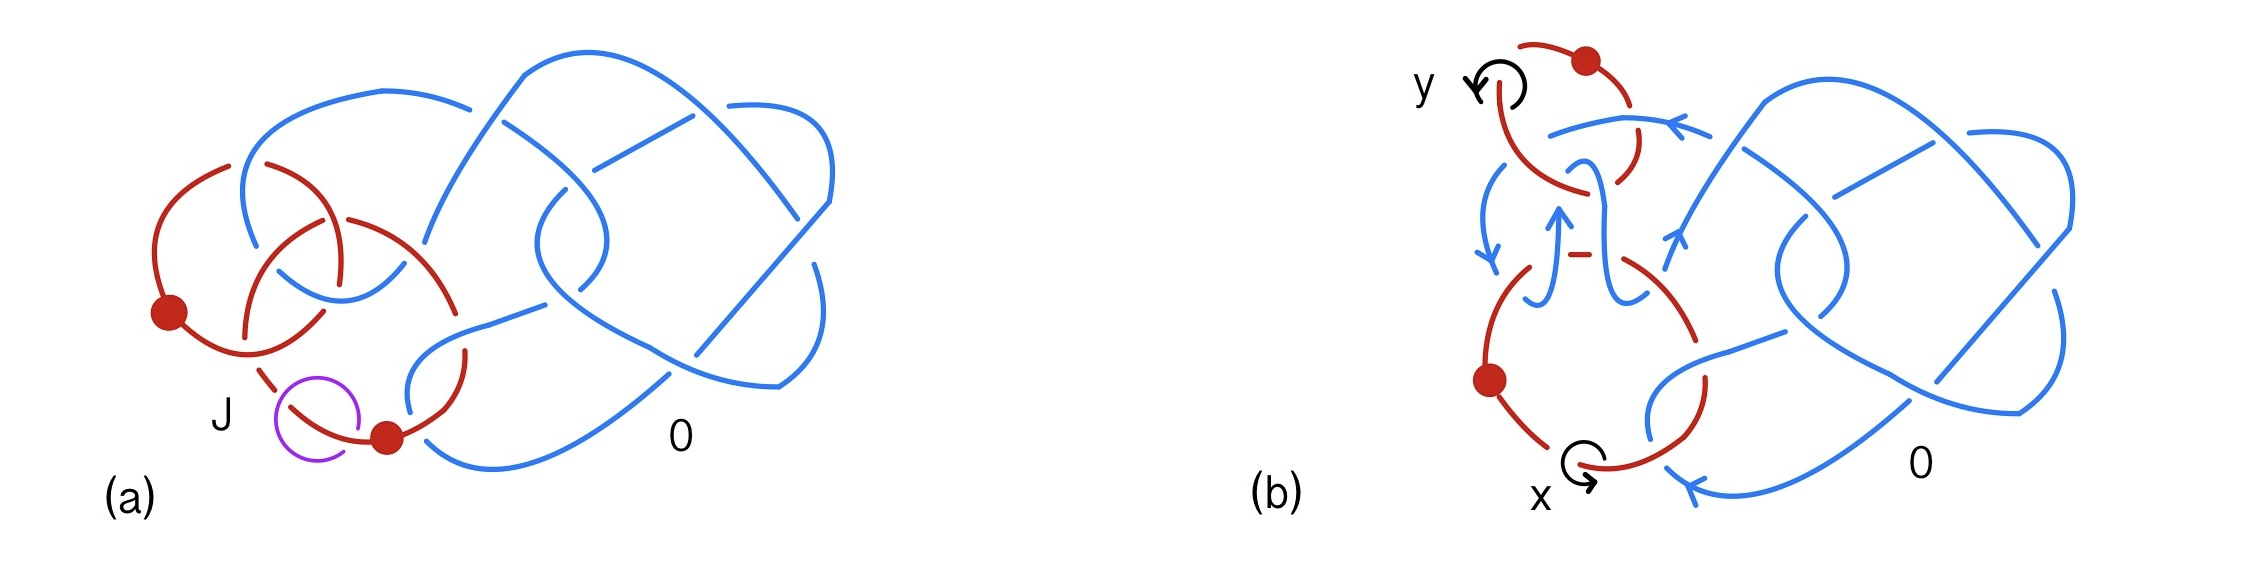
\includegraphics[scale=0.2]{figures/shortcut1.jpeg}
    \caption{Kirby diagram of $\estd$}
    \label{fig:shortcut1}
\end{figure}
We find a presentation of the fundamental groups via the decorated pictures \ref{fig:shortcut1}(b) \ref{fig:shortcut2}(e).
$$
\pi_1(\estd) = \langle x, y \quad | \quad xy^{-1}xyx^{-1} \rangle \cong \Z
$$
$$
\pi_1(\estdi) = \langle x, y \quad | \quad xyx^{-1}y^{-1}yyy^{-1} \rangle \cong \Z
$$
Therefore, the topological isotopy is furnished by Conwell and Powell's theorem \ref{conwa}. Now suppose by contradiction there exist $\phi:  \B^4 \rightarrow \B^4$ carrying $D'$ to $D$.
\begin{figure}[H]
    \centering
    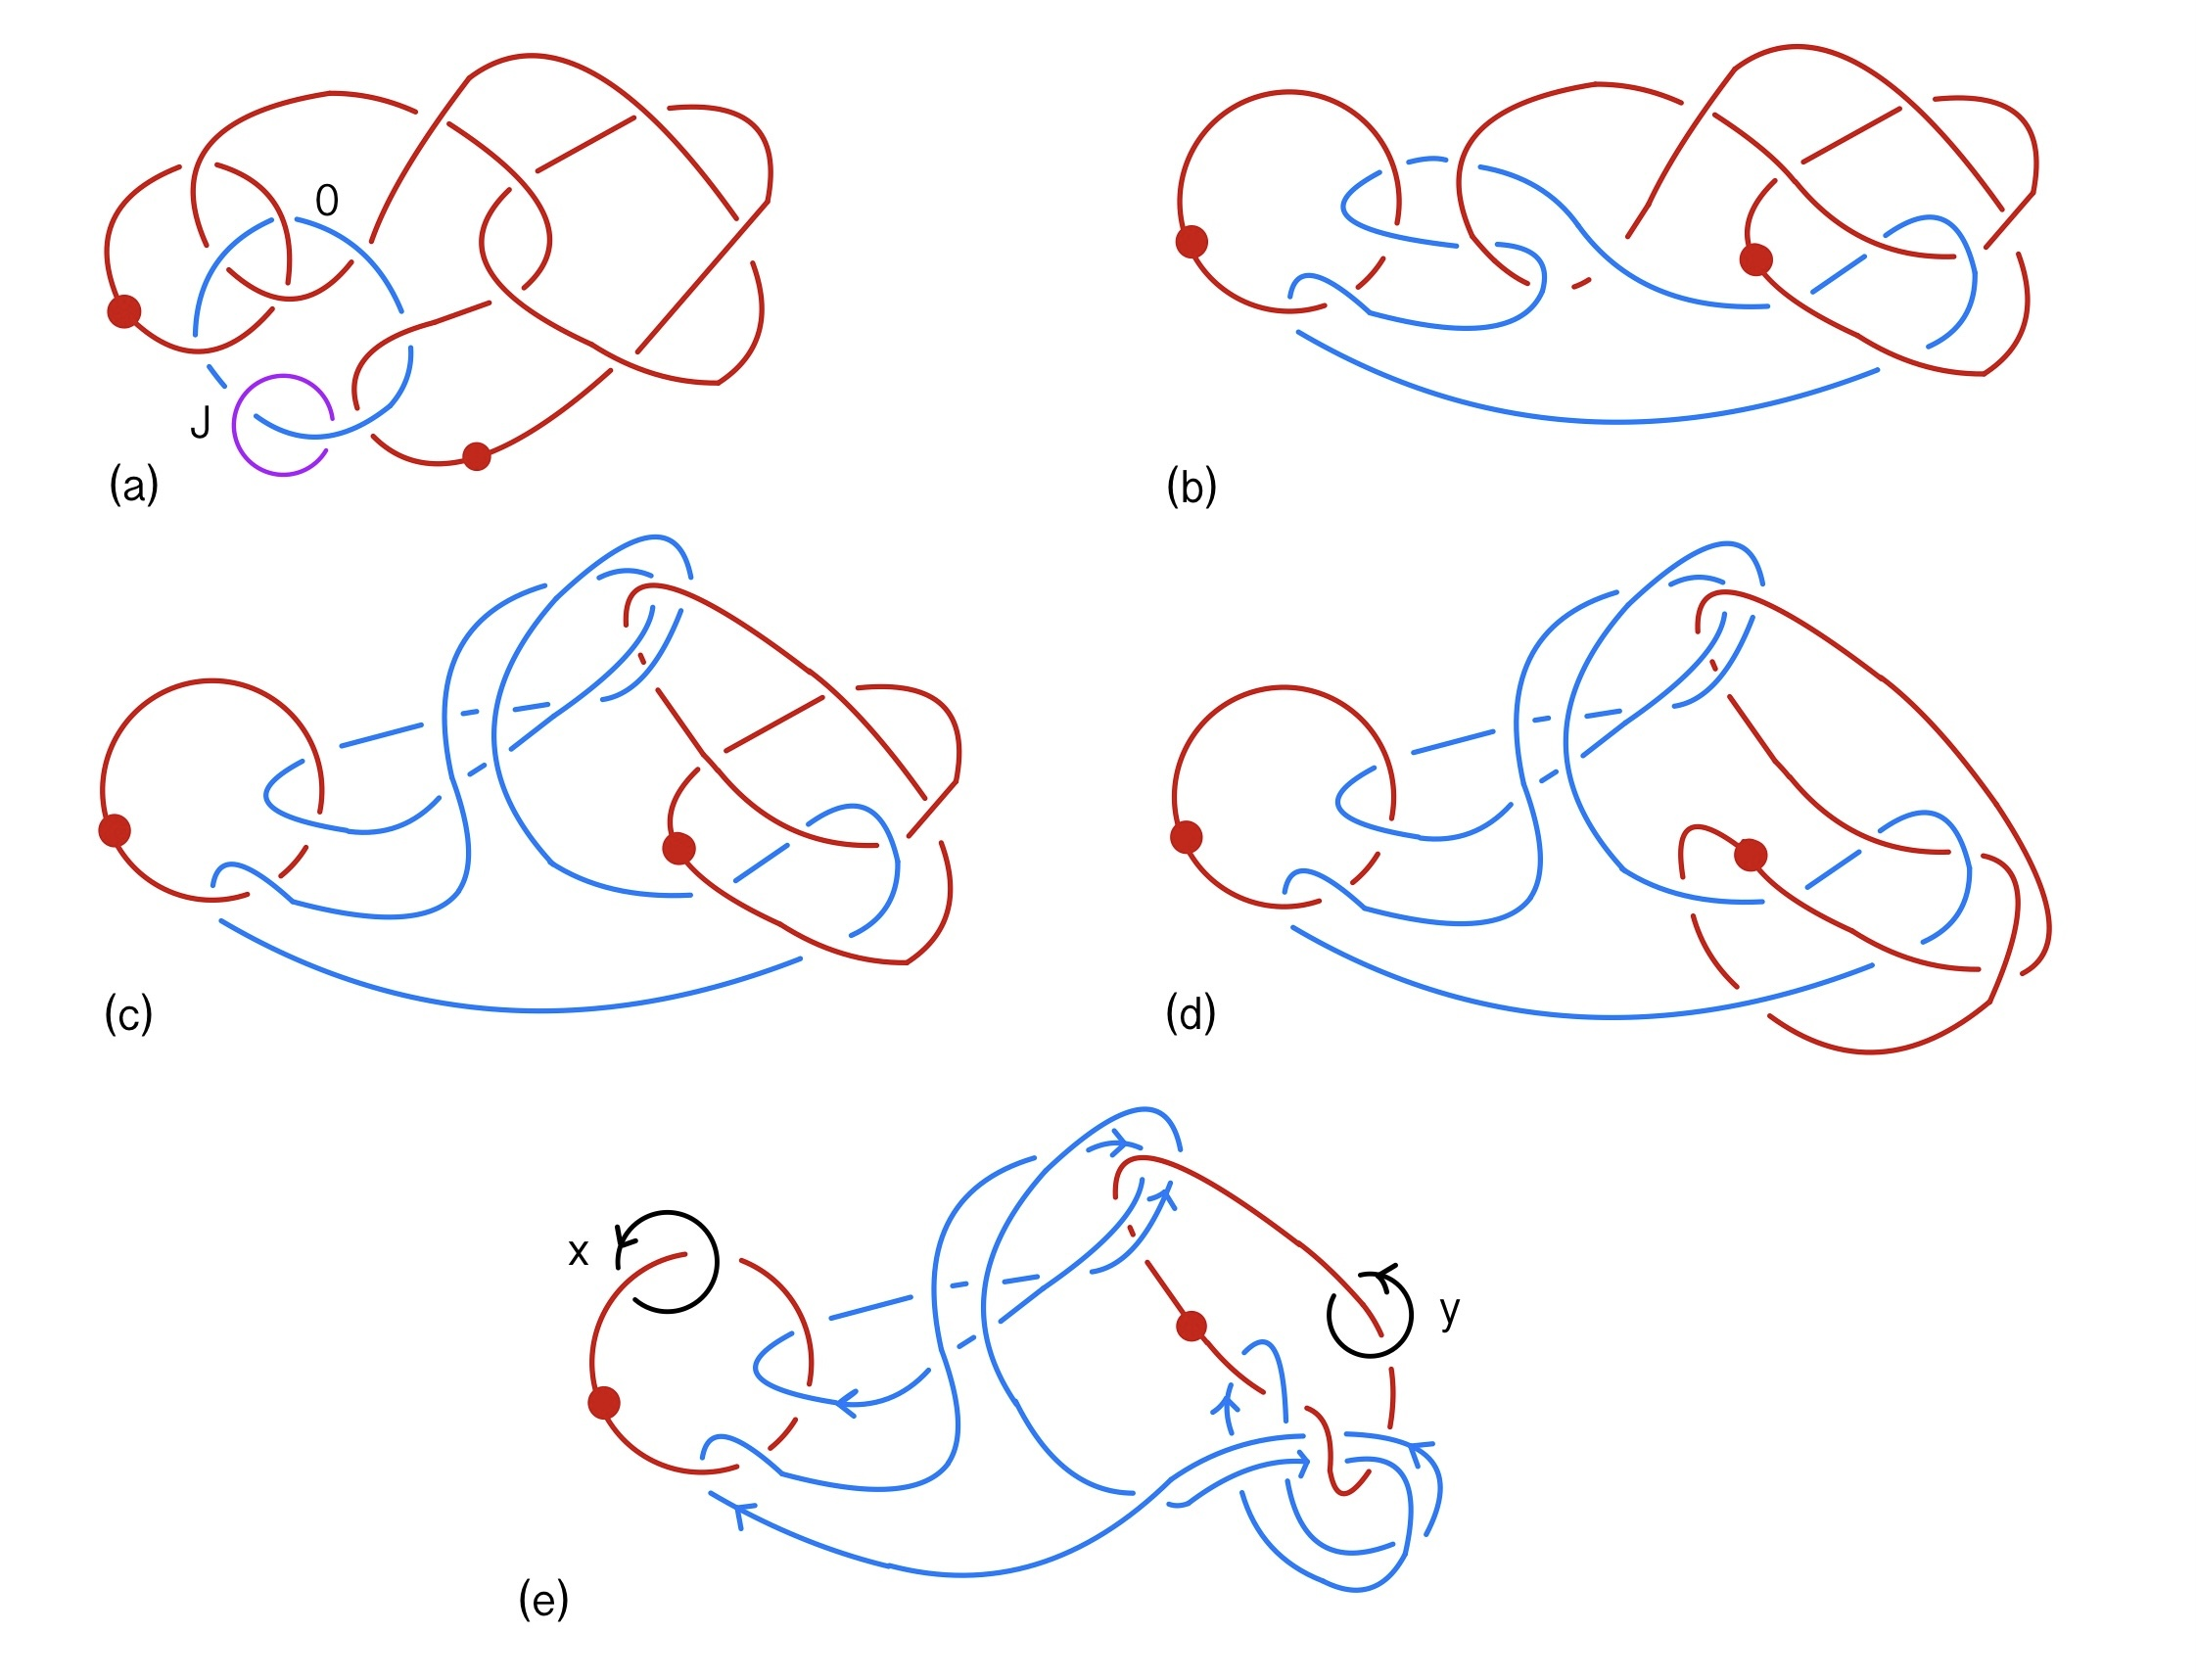
\includegraphics[scale=0.19]{figures/shortcut2.jpeg}
    \caption{Kirby diagram of $\estdi$}
    \label{fig:shortcut2}
\end{figure}
Consider the purple knot $J$ depicted in Figure \ref{fig:shortcut2}(a). Since it does not pass through the $1$-handles, it bounds a disk $\mathfrak{D}'$ in the exterior of $D'$, which is obviously disjoint from $D'$.
At the same way as before, we prove that $\phi$ fixes $\s^3 \setminus \inter$. In particular $J$ is fixed. Therefore, $J$ bounds a disk $\mathfrak{D}$ in $\estd$. 
\begin{obs}Notice that the boundary of $\estd$ is the $0$-surgery on both $A$ and $B$ of Figure \ref{fig:abc}. So $\phi(J)$ inside $\estd$ is actually the purple knot in \ref{fig:shortcut1}(a).
\end{obs}
Now think about what we did before. Switching to the double branched covering has actually simplified the diagram of $\estd$. It reduced the number of $1$-handles so that we could easily recast the diagram in Gompf's standard form. So the underlying idea is to destroy $1$-handles. This can also be achieved by gluing suitable $2$-handles. In this case indeed, we can build a simpler Stein manifold without appealing to the double branched cover. We attach $2$-handles to $\estd$ as in Figure \ref{fig:destroy1}.
\begin{figure}[H]
    \centering
    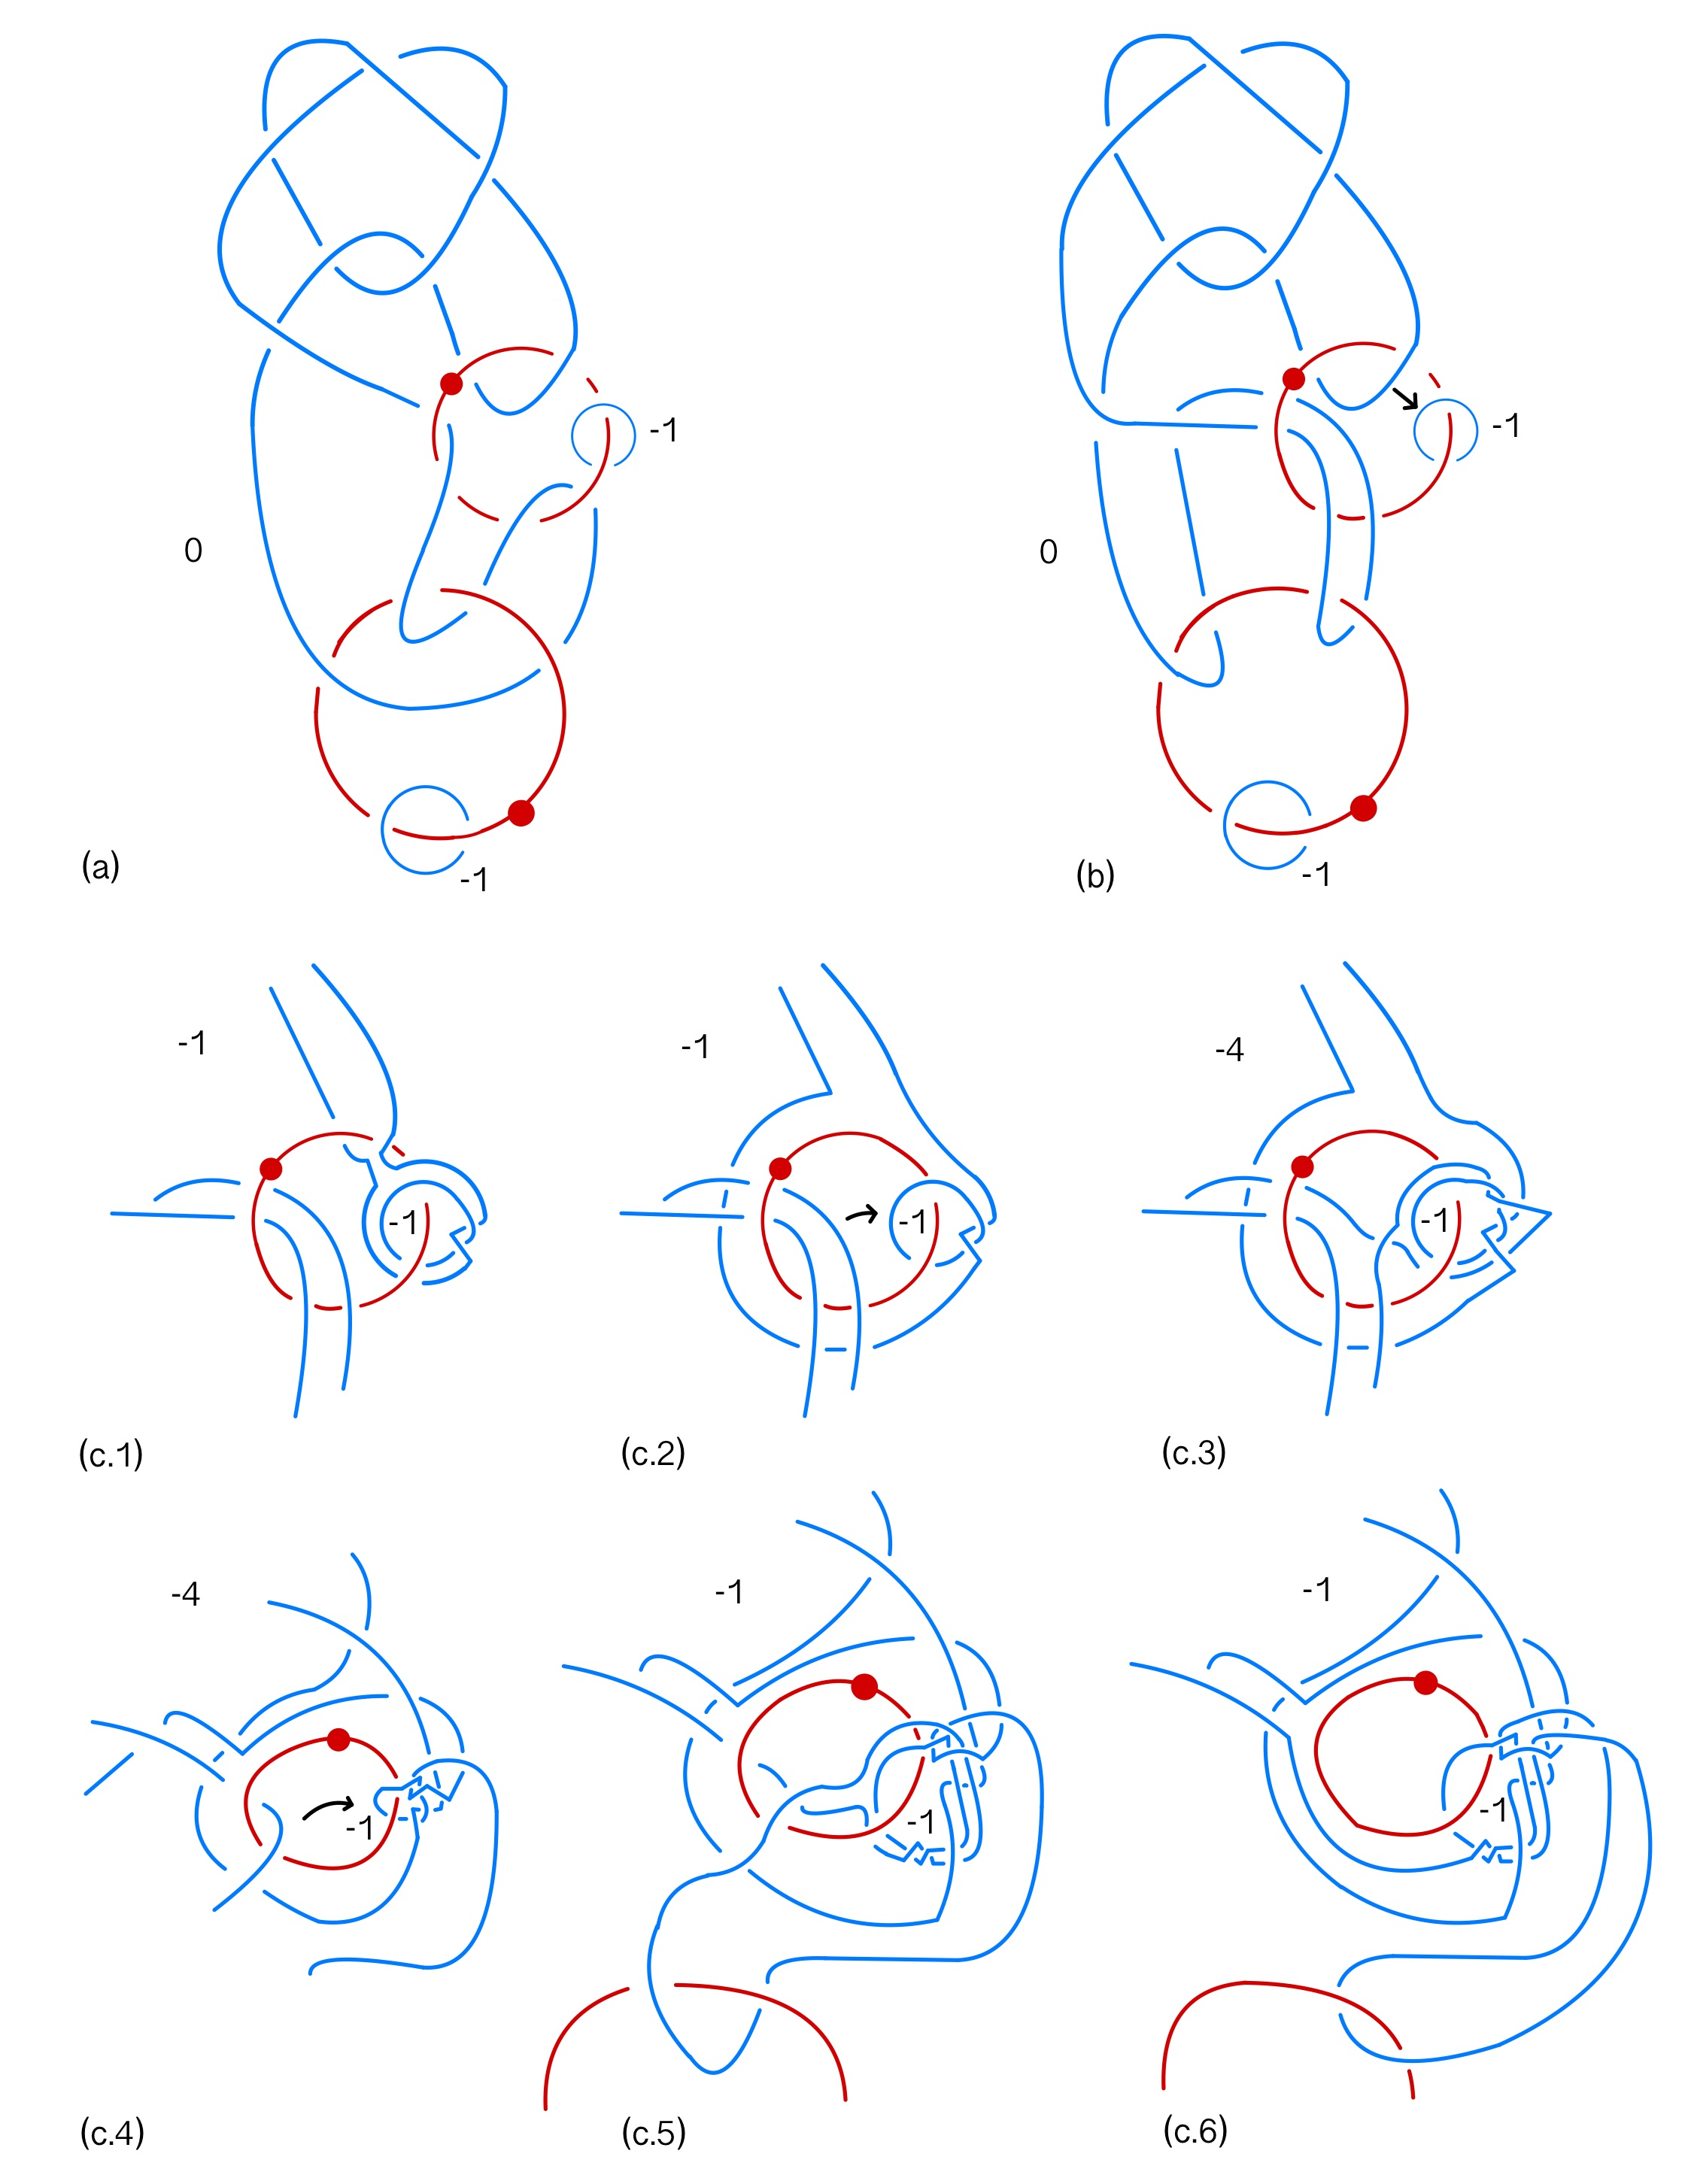
\includegraphics[scale=0.2]{figures/destroy1.jpeg}
    \caption{Simplification of the diagram}
    \label{fig:destroy1}
\end{figure}
\begin{figure}[H]
    \centering
    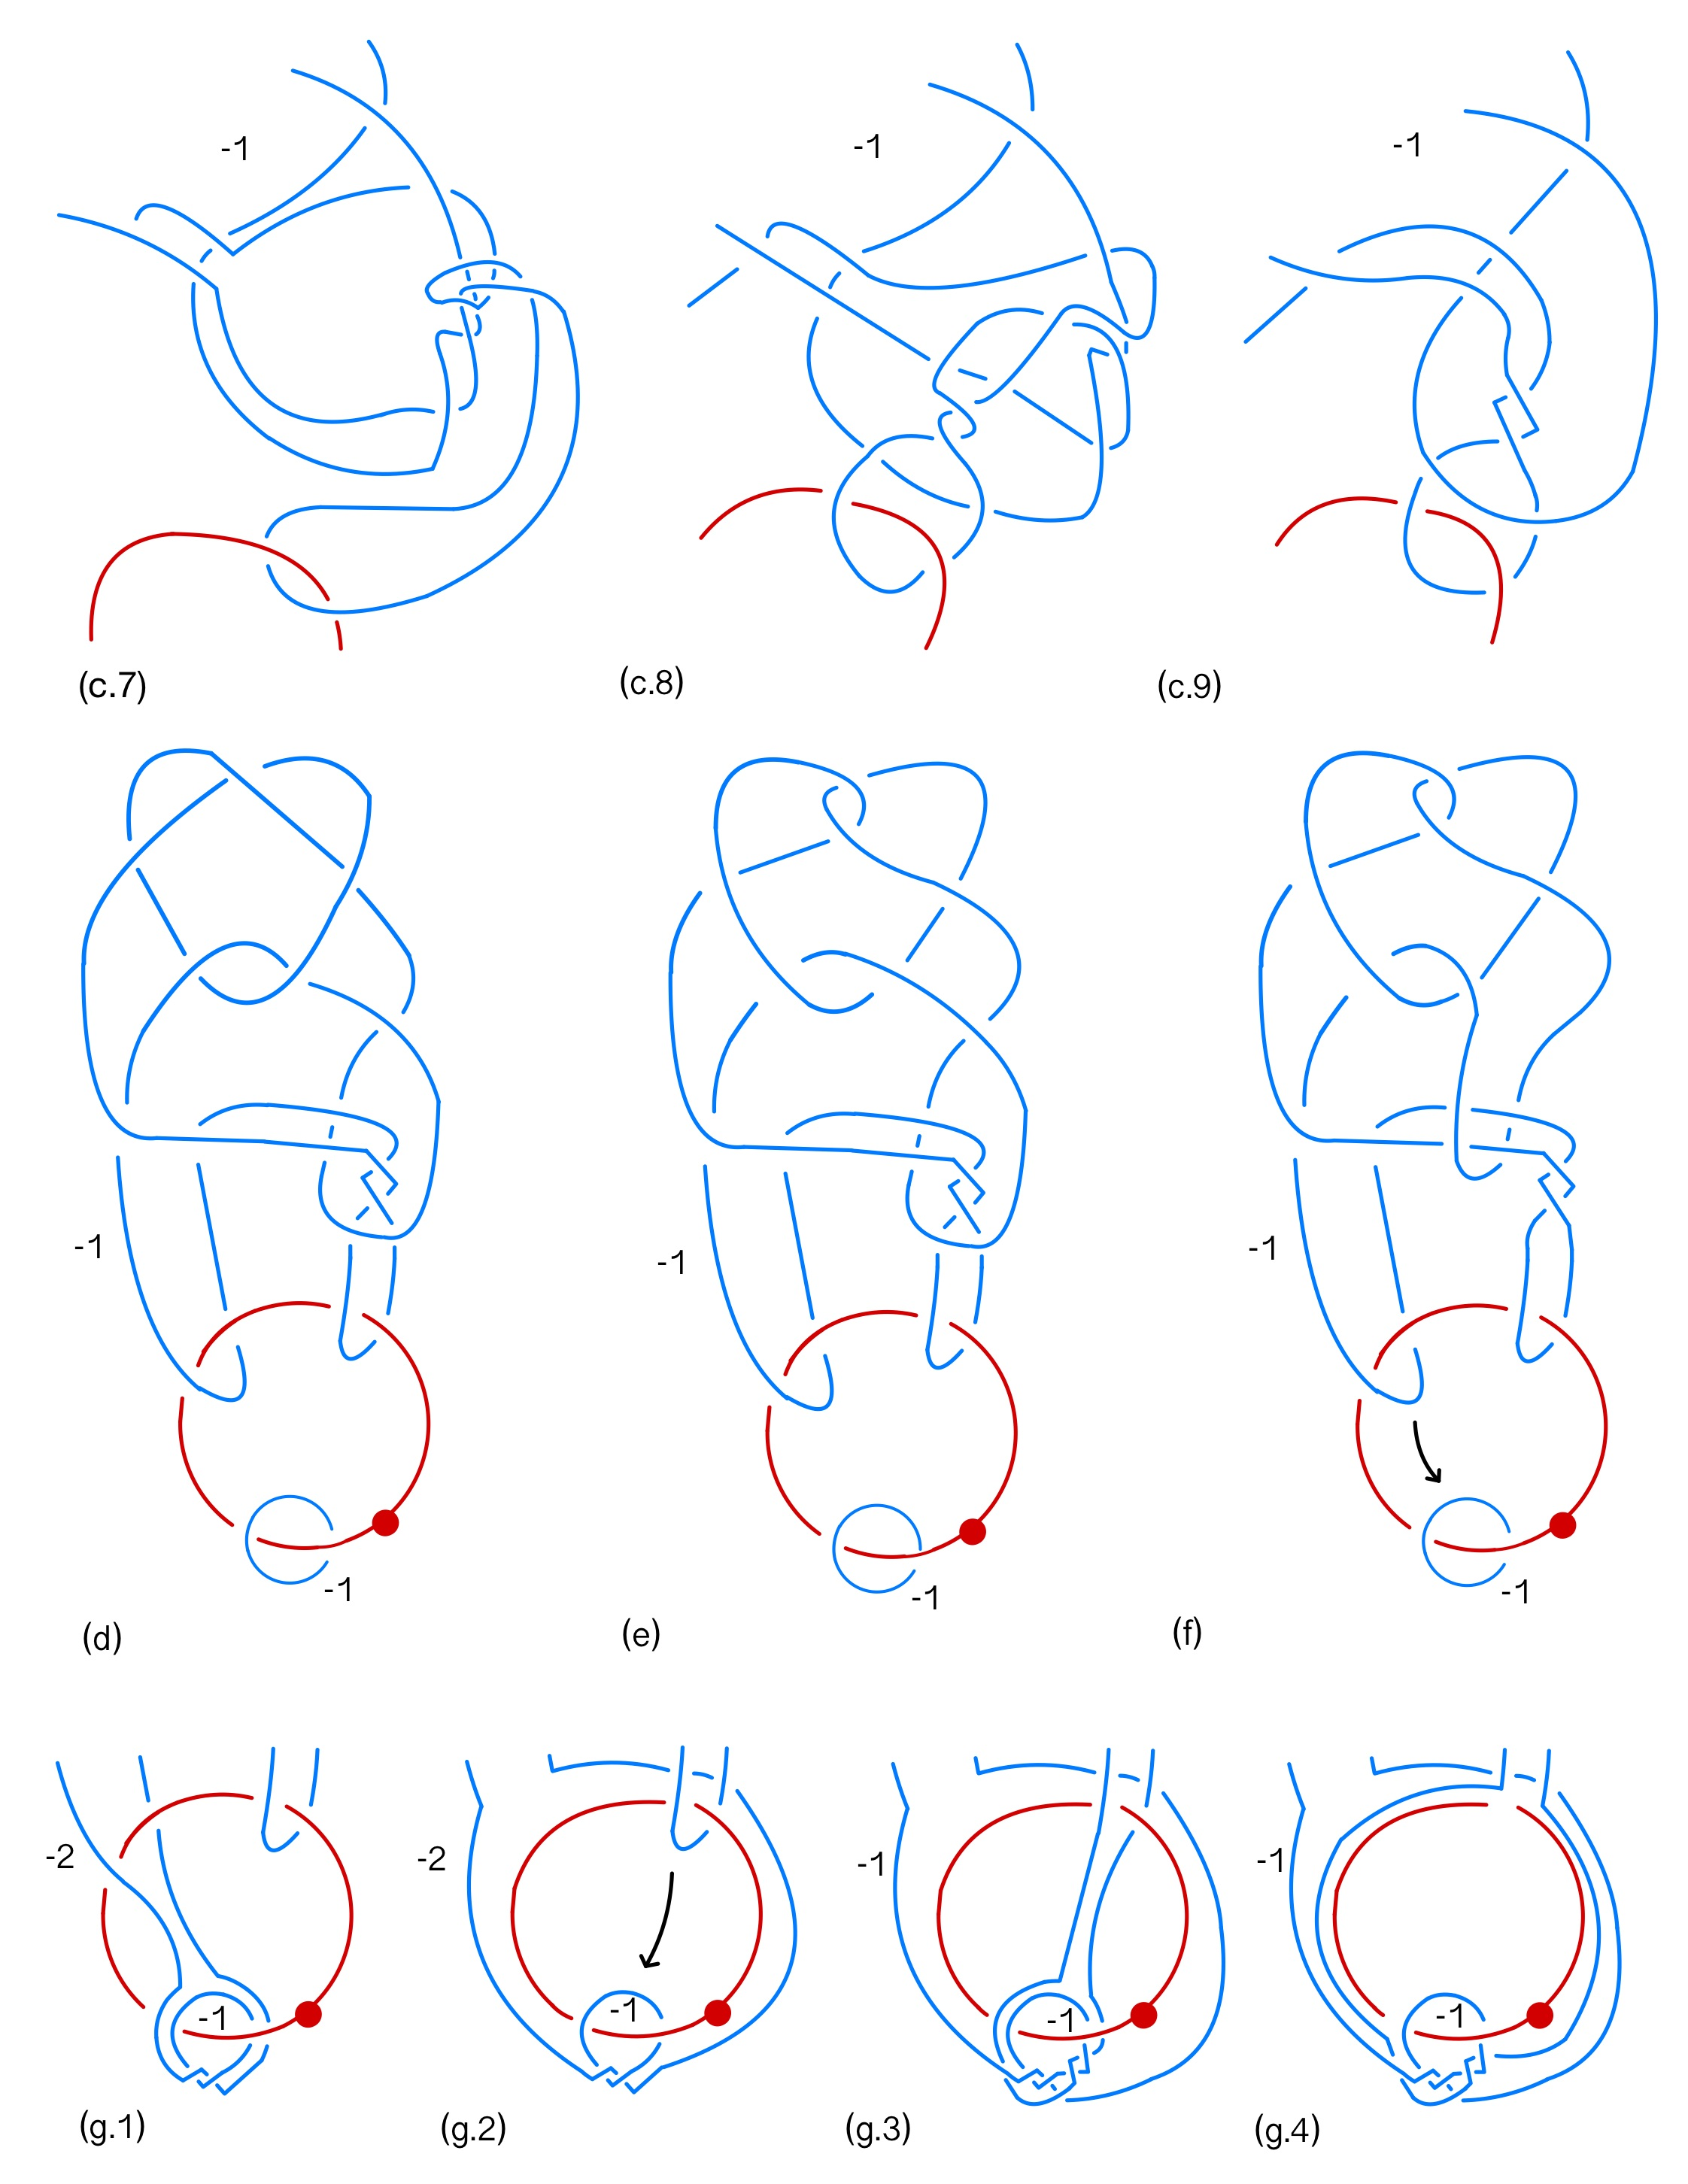
\includegraphics[scale=0.2]{figures/destroy2.jpeg}
    \caption{Further simplification of the diagram}
    \label{fig:destroy2}
\end{figure}
\begin{figure}[H]
    \centering
    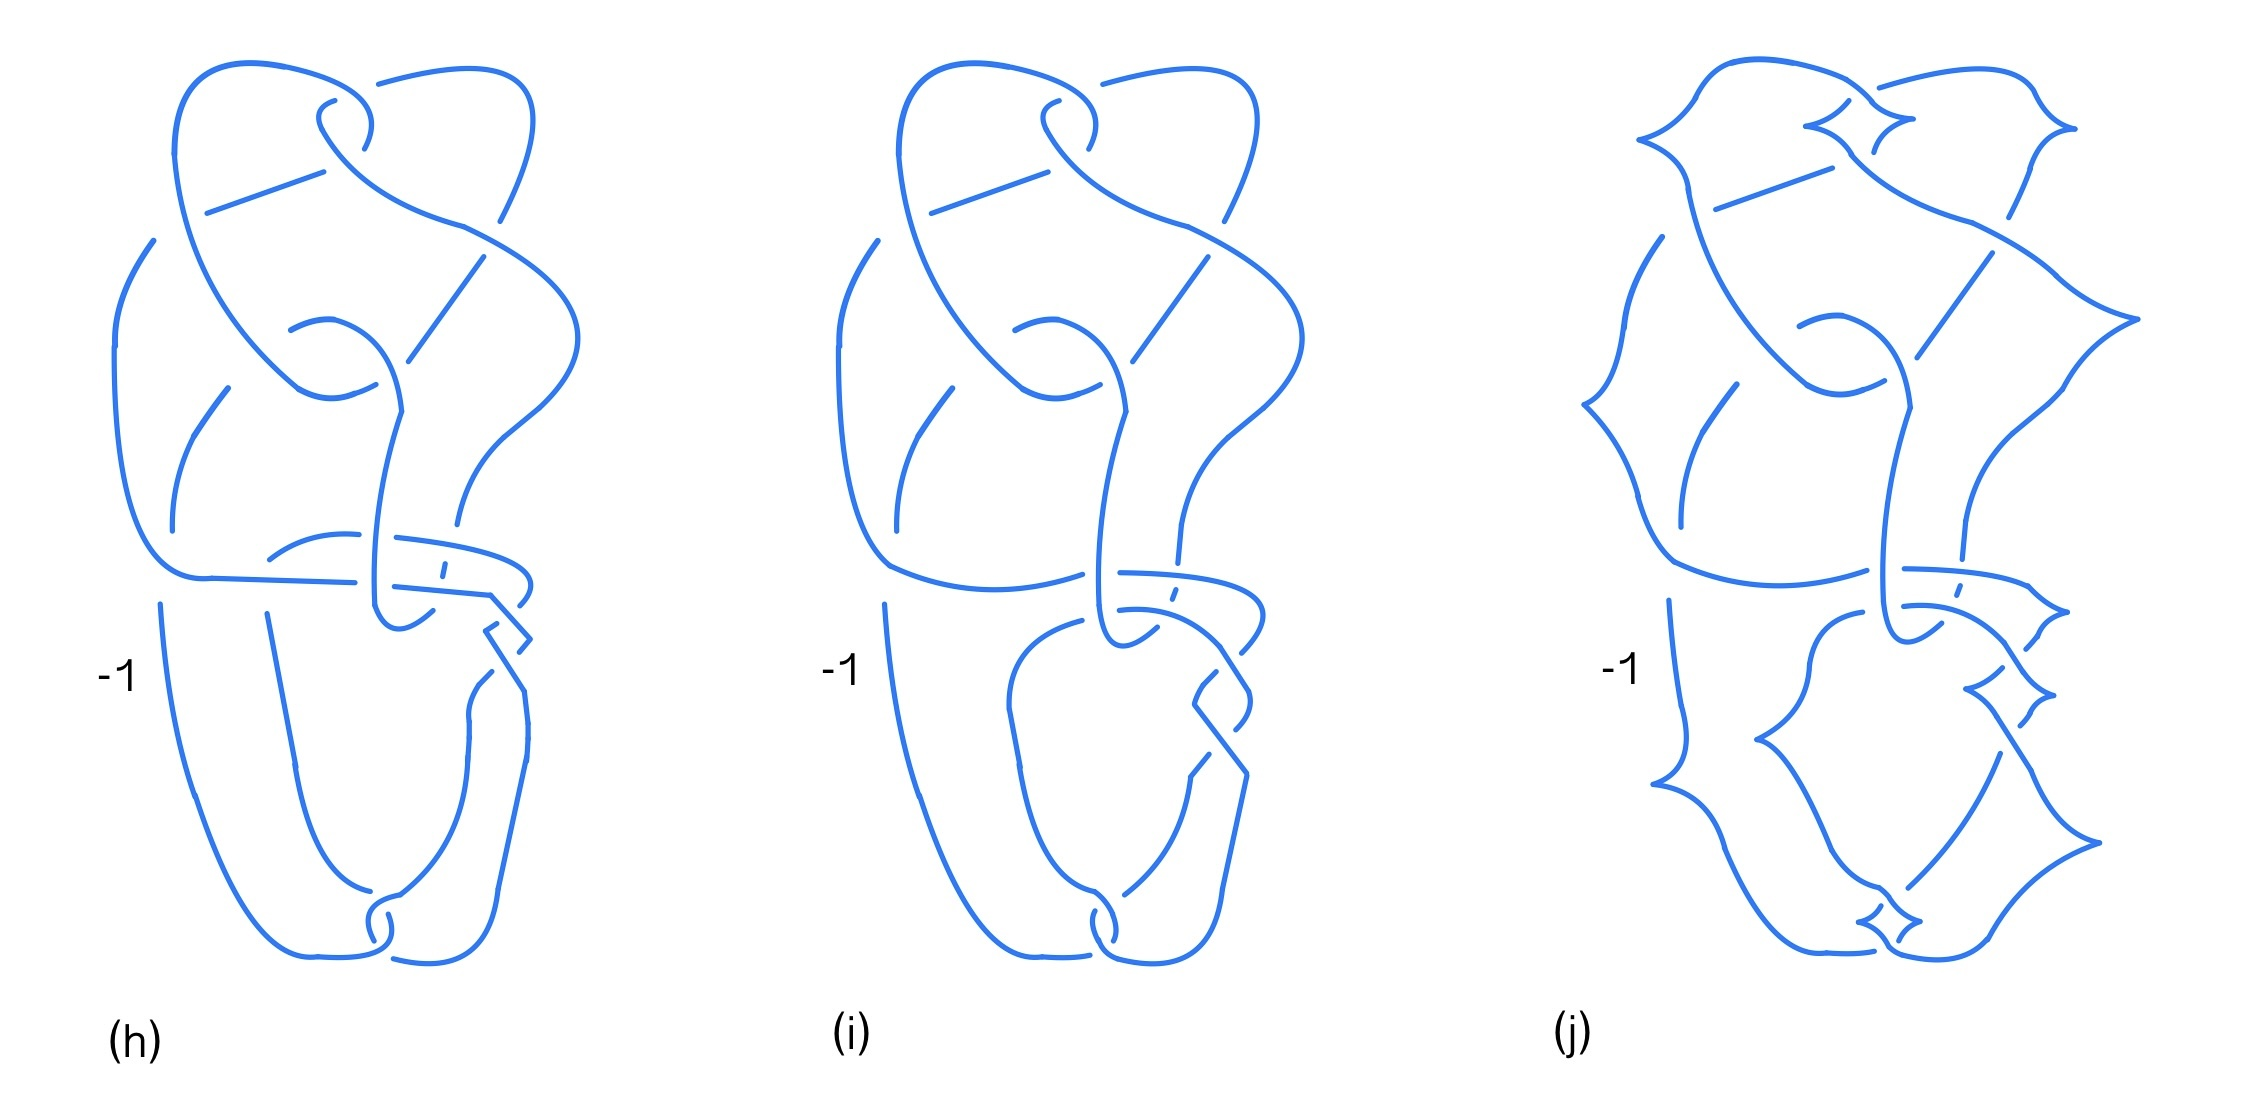
\includegraphics[scale=0.2]{figures/destroy3.jpeg}
    \caption{Knot traces}
    \label{fig:destroy3}
\end{figure}
In the pictures above, we simplify the diagram \footnote{The idea of this proof comes from \cite{hayden2023brunnianexoticsurfacelinks}, Proposition 3.3}.
In order to cancel the upper $1$-handle, we need to perform three handle slides, that are in Figures \ref{fig:destroy1}(c.1), (c.3), (c.5). This time, we have to pay attention to the framing of the $2$-handle that will survive. Call $K_2$ its attaching curve.
$$
f_{K_2} = -1 \qquad \text{after the first slide}
$$ $$
f_{K_2} = - 1 + 2lk(J, K_2) -1 = -4 \quad \text{after the second slide}
$$
And finally we perform a handle subtraction (instead of the usual handle addition) $$
f_{K_2} = - 4 - 2lk(J, K_2) = -1
$$
In Figure \ref{fig:destroy2}(c.7) we cancel the handle pair.
Then, after a sequence of isotopies, we perform two handle slides as in Figures \ref{fig:destroy2}(g.1), (g.3), in order to cancel the other $1$-handle.
We reduced $$W = (\estd)\cup H_2^1 \cup H_2^2$$ to a knot trace. Specifically, in Figure $\ref{fig:destroy3}$(j), $K_2$ is realized as a Legendrain knot with $$w(K_2) = \# \{\text{right cusps}\} = 7$$ So$$
-1 = tb(K_2) - 1
$$
Thus we invoke Eliashberg's characterization theorem \ref{el} to endow $W$ with a Stein structure.
\begin{obs}$\mathfrak{D}$ is capped off with the core of the $2$-handle attached along $J$. 
\end{obs}
This gives rise to a sphere with self intersection $-1$\footnote{$tb(J) = 0$ so $S \cdot S$ equals the framing as argued before.} inside $W$, which is forbidden by proposition \ref{ostruzione}. This leads to the desired contradiction. The disks we found represent a very simple example of exotic disks in $\B^4$. \\ \\
In conclusion, this approach perfectly fits the topological setting, as it is both direct and streamlined. 

\chapter{Construction of Exotic, Symplectic Spheres \\ in Convex 4-Manifolds}
In this chapter, we prove the closed analogue of theorem \ref{prince}.
\begin{thm}\label{king} There exist infinitely many convex symplectic $4$-manifolds, each containing a pair of exotic symplectic spheres.
\end{thm}
The ambient $4$-manifold will be a knot trace. We recall the definition and properties for context. 
\section{Knot Traces}
\begin{defn}Let $K$ be a knot in $\s^3$. The $n$-trace of $K$ is the $4$-manifold obtained by attaching an $n$-framed $2$-handle to $\B^4$ along $K$. It is denoted as $X_n(K)$.
\end{defn}
\begin{obs}We observe that $$
\partial X_n(K) = \s^3_n(K)
$$
\end{obs}
\begin{prop}Suppose $n \neq 0$. Then $Y_n = \s^3_n(K)$ is a rational homology sphere. 
\end{prop}
\proof It suffices to show that $H_1(Y_n, \Q) = H_2(Y_n, \Q) = 0$, as $Y_n$ is connected and closed.
We first compute the homology with integer coefficients and then switch to rational coefficients.
Consider the open sets: $$
U = \s^3 \setminus \nu(K)^{\mathrm{o}} \qquad V = \nu(K) \footnote{We actually consider an enlargement of $\nu(K)$ which is homotopy equivalent to $\nu(K)$}
$$

Then $H_1(U, \Z)$ is generated by a meridian $\mu$ and $H_1(V, \Z)$ is generated by a longitude $\lambda$. Next, examine the following fragment of the Mayer Vietoris exact sequence: 
$$
\begin{tikzcd}
                                 & 0 \arrow[r]                                & H_2(Y_n) \arrow[r, "\partial_1"] & {}            \\
H_1(U\cap V) \arrow[r, "\psi_1"] & H_1(U)\oplus H_1(V) \arrow[r, "\varphi_1"] & H_1(Y_n) \arrow[r, "\partial_0"] & H_0(U \cap V)
\end{tikzcd}
$$ $$
\psi_1(\mu) = n \mu \qquad \psi_1(\lambda) = \lambda
$$
Since $Ker( \partial_0) = 0$\footnote{This can be seen by examining the degree $0$ piece of the sequence}, we obtain
$$
H_1(Y_n) \cong Im(\varphi_1) \cong \Z^2/Im(\psi_1)\cong \Z^2/(\Z \oplus n\Z) \cong \Z/n\Z
$$
In addition $$
H_2(Y_n) \cong Im(\partial_1) \cong Ker(\psi_1) = 0 
$$
We conclude using the Universal coefficient Theorem $$
H_1(Y_n, \Q) \cong \Z/n\Z \otimes \Q = 0
$$as desired.
\endproof
Fix $m<<0$. Let $K_m$ be the knot bounding exotic symplectic disks $D, D'$ we used to prove Theorem \ref{prince}. Consider $X_n = X_n(K_m) = \B^4 \cup H_2$. We build a pair of spheres $S, S'$, by capping off $D, D'$ with the core of the $2$-handle $H_2$.
\begin{figure}[H]
    \centering
    
\includegraphics[scale=0.25]{figures/knottrace.jpeg}
    \caption{The sphere $S$ inside $X_n$}
    \label{fig:knottrace}
\end{figure}
The proof is divided in four steps: \\
(A) For $n \leq -3$, $X_n$ admits a convex symplectic structure, \\
(B) $S$ and $S'$ are symplectic spheres, \\
(C) $S$ and $S'$ are topologically isotopic, \\
(D) Suppose $2 | n$ \footnote{This requirement will be crucial for our proof} and $n <<0$, then $S, S'$ are not smoothly isotopic. \\
\textbf{Proof of (A)} \\
We use the following theorem due to Gay \cite{gay:2-handles}.
\begin{thm} \label{hymn}Let $(X, \omega)$ be a convex $4$-manifold. Suppose that $X' = X \cup H_2$ is constructed by attaching a $n$-framed $2$-handle along the transverse push-off of a Legendrian\footnote{With respect to the contact structure induced by a Liouville vector field} knot $K\subseteq \partial X$. If $n \leq tb(K)-1$, then there exist a symplectic form $\omega'$, such that $(X', \omega')$ is a weak symplectic filling.
\end{thm}
\begin{rem}$K_m$ has a Legendrian realization with $tb(\mathfrak{k}) = -2$ (Figure \ref{fig:tra}(a)). So the requirement of the previous Theorem is satisfied for $n \leq -3$.
\end{rem}
Thus for such values of $n$, $X_n$ admits a symplectic form $\omega'$, such that $\partial X_n = \s^3_n(K_m)$ is weakly symplectically filled by $X_n$.
Then by Proposition \ref{osha}, up to a small deformation of $\omega'$, $X_n$ admits a convex symplectic structure, as desired. \\ \\
\textbf{Proof of (B)} \\
We need to prove that $D$ and $D'$ can be capped off symplectically. 
First, observe that the core disk inherits an area form from the $2$-handle, and therefore it is symplectic. 
\begin{prop}\label{tool4} Using the notations above, suppose that $S$ is obtained by capping off a symplectic surface $F\subseteq \B^4$ with the core of the $2$-handle attached along $\partial F = K$. If $F$ is cylindrical near its boundary\footnote{In our case, this technical requirement is satisfied, see the construction in Lemma \ref{cob}}, then $S$ is symplectic in $(X_n, \omega')$.
\end{prop}
The latter, can be proved by analyzing the explicit gluing maps, and it is carried out in section 7.2 of \cite{bowden2010}. \\ \\
\textbf{Proof of (C)} \\
Since $D$ and $D'$ are topologically isotopic (relatively to the boundary), then the spheres obtained by capping them off are also topologically isotopic. \\ \\
\textbf{Proof of (D)} \\
We mimic the same strategy we used to prove \ref{prince}. Assume, for the sake of contradiction, that there exists a diffeomorphism $\varphi: X_n \rightarrow X_n$ such that $\varphi (S') = S$.
\begin{lem}\label{tool8} Let $n<<0$ and either $m<<0$ or $m=0$. Then every self diffeomorphism of $\partial X_n= \s^3_n(K_m)$ is isotopic to the identity.
\end{lem}
\proof
For $m<<0$ or $m= 0$, $\s^3 \setminus K_m$ is an asymmetric hyperbolic manifold \ref{app}. Thus, by Lemma \ref{cuspi}, $\s^3_n(K_m)$ (which is the Dehn filling of $\s^3 \setminus K_m$) is also hyperbolic and asymmetric for $n <<0$.
We conclude using the fact that every diffeomorphism of an hyperbolic $3$ manifold is isotopic to an isometry.
\endproof
Using the same notations employed in the proof of \ref{prince}, we recall that $J$ (depicted in Figure \ref{fig:km}) bounds a disk $\mathfrak{D'}\subseteq \estd$. As $J \subseteq \s^3 \setminus K_m$ is unaffected from Dehn surgery, it still bounds a disk $\mathfrak{D'} \subseteq X_n$. Moreover, $\mathfrak{D'}$ is disjoint from $S'$. Since $\varphi(J) = J$, it follows that $$
\varphi(\mathfrak{D'}) = \mathfrak{D}
$$
is a disk bounding $J$ and disjoint from $S$.
\section{Describing the Double Branched Covering of an $n$-Trace}
In this section, we obstruct the existence of $\mathfrak{D}$, using the same techniques we used in sections \ref{buffet} \ref{summon}. 
\begin{lem}\label{warietto} $H_1(X_n \setminus S) \cong \Z/n\Z$
\end{lem}
\proof Let $\nu(S)$ be a tubular neighbourhood of $S$ inside $X_n$. Consider the following fragment of Mayer-Vietoris exact sequence: 
$$
\begin{tikzcd}
H_2(X_n) \arrow[r] & H_1(\nu(S) \setminus S) \arrow[r, "\phi"] & H_1(X_n \setminus S)\oplus H_1(\nu(S)) \arrow[r] & 0
\end{tikzcd}$$
Since $H_1(\nu(S) \setminus S)$ is generated by a meridian $\mu$ and $\phi$ is surjective, $\mu$ also generates $H_1(X_n \setminus S)$.
Notice that the parallel pushoff of $K_m$, which is $\lambda + n\mu$, bounds a pushoff of the $2$-handle's core disk. As $[\lambda] = 0 \in H_1(X_n \setminus S)$, it follows that $n[\mu] = 0 \in H_1(X_n \setminus S)$, as desired.
\endproof
This leads to the following theorem.
\begin{thm}\label{wario}
If $2|n$, then the double branched covering of $X_n$ along $S$ exists and it is unique.
Moreover $$
\Sigma(X_n, S) = \Sigma(\B^4, D) \cup H'_2
$$ with the $2$-handle attached along the lift of $K$ with framing $\frac{n}{2}$.
\end{thm}
\proof
By the previous lemma, $H_1(X_n \setminus S) \cong \Z/n\Z$ has a unique index $2$ subgroup. Thus we may repeat the same argument used in section \ref{covers} to prove existence and uniqueness. Now we describe the handle decomposition of $\Sigma(X_n, S)$.
Since $X_n = \B^4 \cup H_2$, we obtain: $$
\Sigma(X_n, D \cup (\D^2 \times 0) ) = \Sigma(\B^4, D) \cup \Sigma(\D^2\times \D^2, \\\D^2 \times 0) = \Sigma(\B^4, D) \cup (\D^2\times \D^2) 
$$
Let $\tilde{K}$ be an arbitrary lift of $K$. We observe that the attaching region of $H_2$, which is $\nu(K)$, lifts to $\nu(\tilde{K}) \subseteq \partial\Sigma(\B^4, D)$.
Therefore $\Sigma(X_n, S)$ is constructed from $\Sigma(\B^4, D)$ by attaching a $2$-handle along $\tilde{K}$. It remains to determine the attaching framing.
\begin{obs}The branched covering map, restricted to $\nu(\tilde{K)}$, in complex coordinates, is given by: $$
\nu(\tilde{K)} \cong \s^1 \times \D^2 \rightarrow \nu(K) \cong \s^1 \times \D^2
$$ $$
(x, z) \rightarrow (x, z^2)
$$
\end{obs}
Thus, the induced map on the first homology groups of the boundaries is defined as: $$
\lambda \rightarrow \lambda \qquad \qquad [0 \times \partial \D^2] \rightarrow 2[0 \times \partial \D^2]
$$
This proves that the framing coefficient is $\frac{n}{2}$.
\endproof
As a result, a handle diagram for $\Sigma(X_n, S)$ is obtained by attaching a $\frac{n}{2}$-framed $2$-handle, along $\tilde{K}$, to a handle diagram of $\Sigma(\B^4, D)$.
Let $TB(K)$ denote the maximal Thurston-Bennequin number of $K$. 
\begin{obs}If $$
\frac{n}{2} \leq TB(\tilde{K}) -1
$$
there exists a Legendrian realization $\mathfrak{\tilde{k}}$ of $\tilde{K}$ such that $$
\frac{n}{2} = tb(\mathfrak{\tilde{k}})-1 \footnote{It is obtained with a sequence of (negative) stabilizations}
$$
\end{obs}
Thus, for such values of $n$, $\Sigma(X_n, S)$ admits a Stein structure.
The final argument can be repeated verbatim. We attach a $-1$-framed $2$-handle to $\Sigma(X_n, S)$ along $\tilde{J}$, a lift of $J$, to obtain a sphere with self intersection $-1$. Such sphere is forbidden in Stein $4$-manifolds. Hence we get to the desired contradiction. 





\chapter{Higher Genus Surfaces}
In this chapter, we construct exotic surfaces with arbitrary genus. We discuss how to adapt the proofs we have seen in the previous chapters to the positive genus case. \\ \\

Below, we present the final form of the main theorems of chapters 3 and 4.
\begin{thm}Let $g \geq 0$. There exist infinitely many transverse knots in $(\s^3, \xi_{st})$, each bounding a pair of exotic, genus $g$, symplectic surfaces in $(\B^4, \omega_{st})$.
\end{thm}
\begin{thm} \label{ulti} Let $g \geq 0$. There exist infinitely many convex symplectic $4$-manifolds containing a pair of exotic, closed, symplectic, genus $g$ surfaces.
\end{thm}




We begin by proving the non-closed case. Instead of constructing such surfaces from scratch, we will attach bands to the previously found exotic disks (i.e., perform the connected sum with a genus-$g$ surface).
\section{Holomorphic Curves Bounded by $\torus$}
In this section, we construct a genus-$g$ holomorphic \footnote{The usefulness of the holomorphic structure will become evident in the subsequent steps.} curve embedded in $\B^4$, with $g>0$. 
Consider the holomorphic function $$
f: \C^2 \rightarrow \C
$$ $$
(z_1, z_2) \rightarrow z_1^2 + z_2^{2g+1}
$$
\begin{as} Let $S_{\epsilon}\subseteq\C^2$ be the radius $\epsilon$ sphere centered in $0$, and $V = f^{-1}(0)$. Then $$
V \cap S_{\epsilon} = \torus
$$
\end{as}
\proof
Let $(z_1, z_2) \in V \cap S_{\epsilon}$. Then the following equations hold: $$
|z_1|^2+|z_2|^2 = \epsilon
$$ $$
|z_1|^2 = |z_2|^{2g+1}
$$
Thus $|z_1|$ and $|z_2|$ are equal to two costants $c_1, c_2$. An easy computation shows that all the points of the form$$
(c_1e^{(2g+1)i\theta}, c_2e^{2\pi i+\frac{\pi i}{2g+1}}) \qquad \theta \in [0, 2\pi]
$$ satisfy both the equations defining $V$ and $S_{\epsilon}$. Hence the thesis.
\endproof
Now, since $\nabla f(z) \neq 0 \quad \forall z \neq 0$, we can deform $V$ into a smooth complex curve, defined as: $$
F_0 = \{z_1^2 + z_2^{2g+1} = \epsilon\}
$$
for some small $\epsilon > 0$.
\begin{obs}  $\partial F_0 = \torus$ and $F_0$ has genus $g$, as required.
\end{obs}
Let $h: F_0 \rightarrow \B^4$ be an embedding. \\
Complex curves in Stein $4$-manifolds carry a natural positive symplectic form given by
the pullback of $\omega_{\phi}$ via $h$ \cite{eliashberg2012stein}. 
\begin{note} Symplecticity of $F_0$ can also be proven via Lemma \ref{cob} and the following transverse link movie:
\begin{figure}[H]
    \centering
    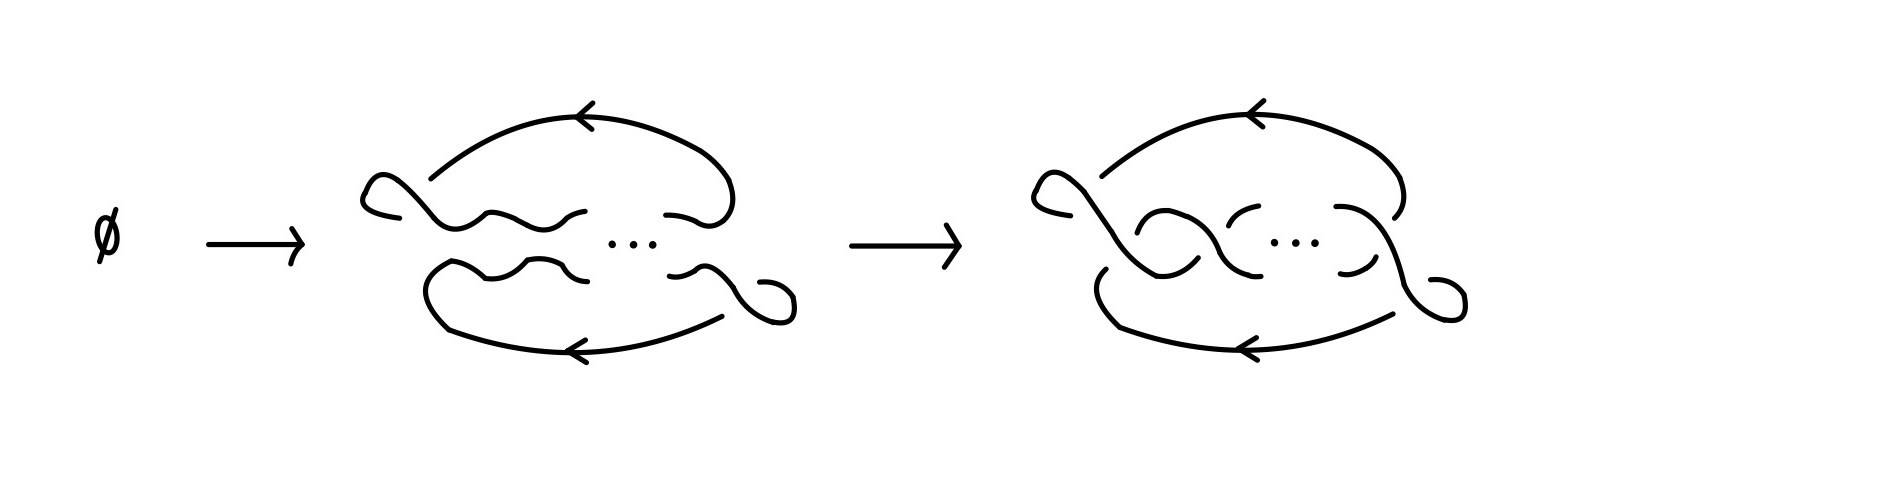
\includegraphics[scale=0.25]{figures/movie.jpeg}
    \caption{A transverse link movie for $F_0$}
    \label{fig:movie}
\end{figure}
\end{note}
Let $F = F_0 \natural D$ and $F' = F_0 \natural D'$ (where $D, D'$ are the exotic disks of Theorem \ref{prince}).
\begin{note} $\partial F = \partial F' = K_m \#\torus$ are transverse knots in $(\s^3, \xi_{st})$.
\end{note}
We claim that $F, F'$ is an exotic pair of genus $g$ symplectic surfaces.
Since $D$ and $D'$ are topologically isotopic, the same holds for $F$ and $F'$. \\ \\
To prove that $F, F'$ are symplectic, we observe that the connected sum of two knots can be achieved using the saddle move shown in Figure \ref{fig:moves}(b), and then use Lemma \ref{cob}.  \\ \\
It remains to show that $F$ and $F'$ are not smoothly isotopic (relatively to the boundary). We mimic the strategy used for the case $g=0$. 
Assume by contradiction that there exists a diffeomorphism $\varphi: \B^4 \rightarrow \B^4$ such that $\varphi(F') = F$. Hence $\varphi (K_m \# \torus) = K_m \# \torus$. 
We aim to prove that $J \subseteq \s^3 \setminus (K_m \# \torus)$ is fixed by $\varphi$, up to isotopy. To this end, we study the set of diffeomorphisms of $Y = \s^3 \setminus (K_m \# \torus)$, up to isotopy. 
\begin{lem} \label{techhh} Suppose that $m = 0$ or $m<<0$.
Then every self diffeomorphism of $\s^3 \setminus (K_m \# \torus)$ restricts to the identity on $\s^3 \setminus \inter$, up to isotopy.
\end{lem}
Unfortunately, $Y$ is not hyperbolic (so we can't use the same argument of Lemma \ref{technic}) . However, we can decompose $Y$ into simpler pieces.
In this section, we prove Lemma \ref{techhh} using the $JSJ$ decomposition tool, reducing the argument to that of Lemma \ref{technic}.
\\ \\
First, we briefly review the $JSJ$ decomposition following Hatcher's notes \cite{hatcher2002notes}. Let $Y$ be a $3$ manifold. 
\begin{defn}$Y$ is said to be irreducible if every embedded sphere $S \rightarrow Y$ bounds a ball $\B^3 \subseteq Y$. 
\end{defn}
\begin{ex} For every knot $K$, $\s^3 \setminus K$ is an irreducible manifold. In fact, every sphere bounds two balls in $\s^3$, one of which contains $\nu(K_m)$. Hence the other is contained in $\s^3 \setminus K$.
\end{ex}
\begin{defn}Let $F \rightarrow Y$ be an embedded surface other than $\s^2$ or $\D^2$.
$F$ is said to be incompressible if for each disk $D \subseteq Y$ with $D \cap F = \partial D$, there exists a disk $D' \subseteq F$ such that $\partial D = \partial D'$ (as in Figure \ref{fig:seifert}(a)).
\end{defn}
\begin{ex}\label{heart} Let $V$ be a unknotted torus, and let $P\subseteq V$ be an essential\footnote{It means that $P$ intersects every meridional disk} knot. Consider a diffeomorphism $h : V \rightarrow \nu(C)$. 
$$
S  (C, P) = h(P) \subseteq \nu(C)
$$
is called a satellite knot with companion $C$ and pattern $P$. \\
The torus $h(\partial V)$ is incompressible in the exterior of $S(C, P)$. \cite{schultens2014introduction}, cfr \cite{gabai1987foliations}. 
\end{ex}
The concepts of knot complements and $JSJ$ decomposition are intimately related; we refer the interested reader to \cite{budney2006jsj}. 
\begin{figure}[H]
    \centering
    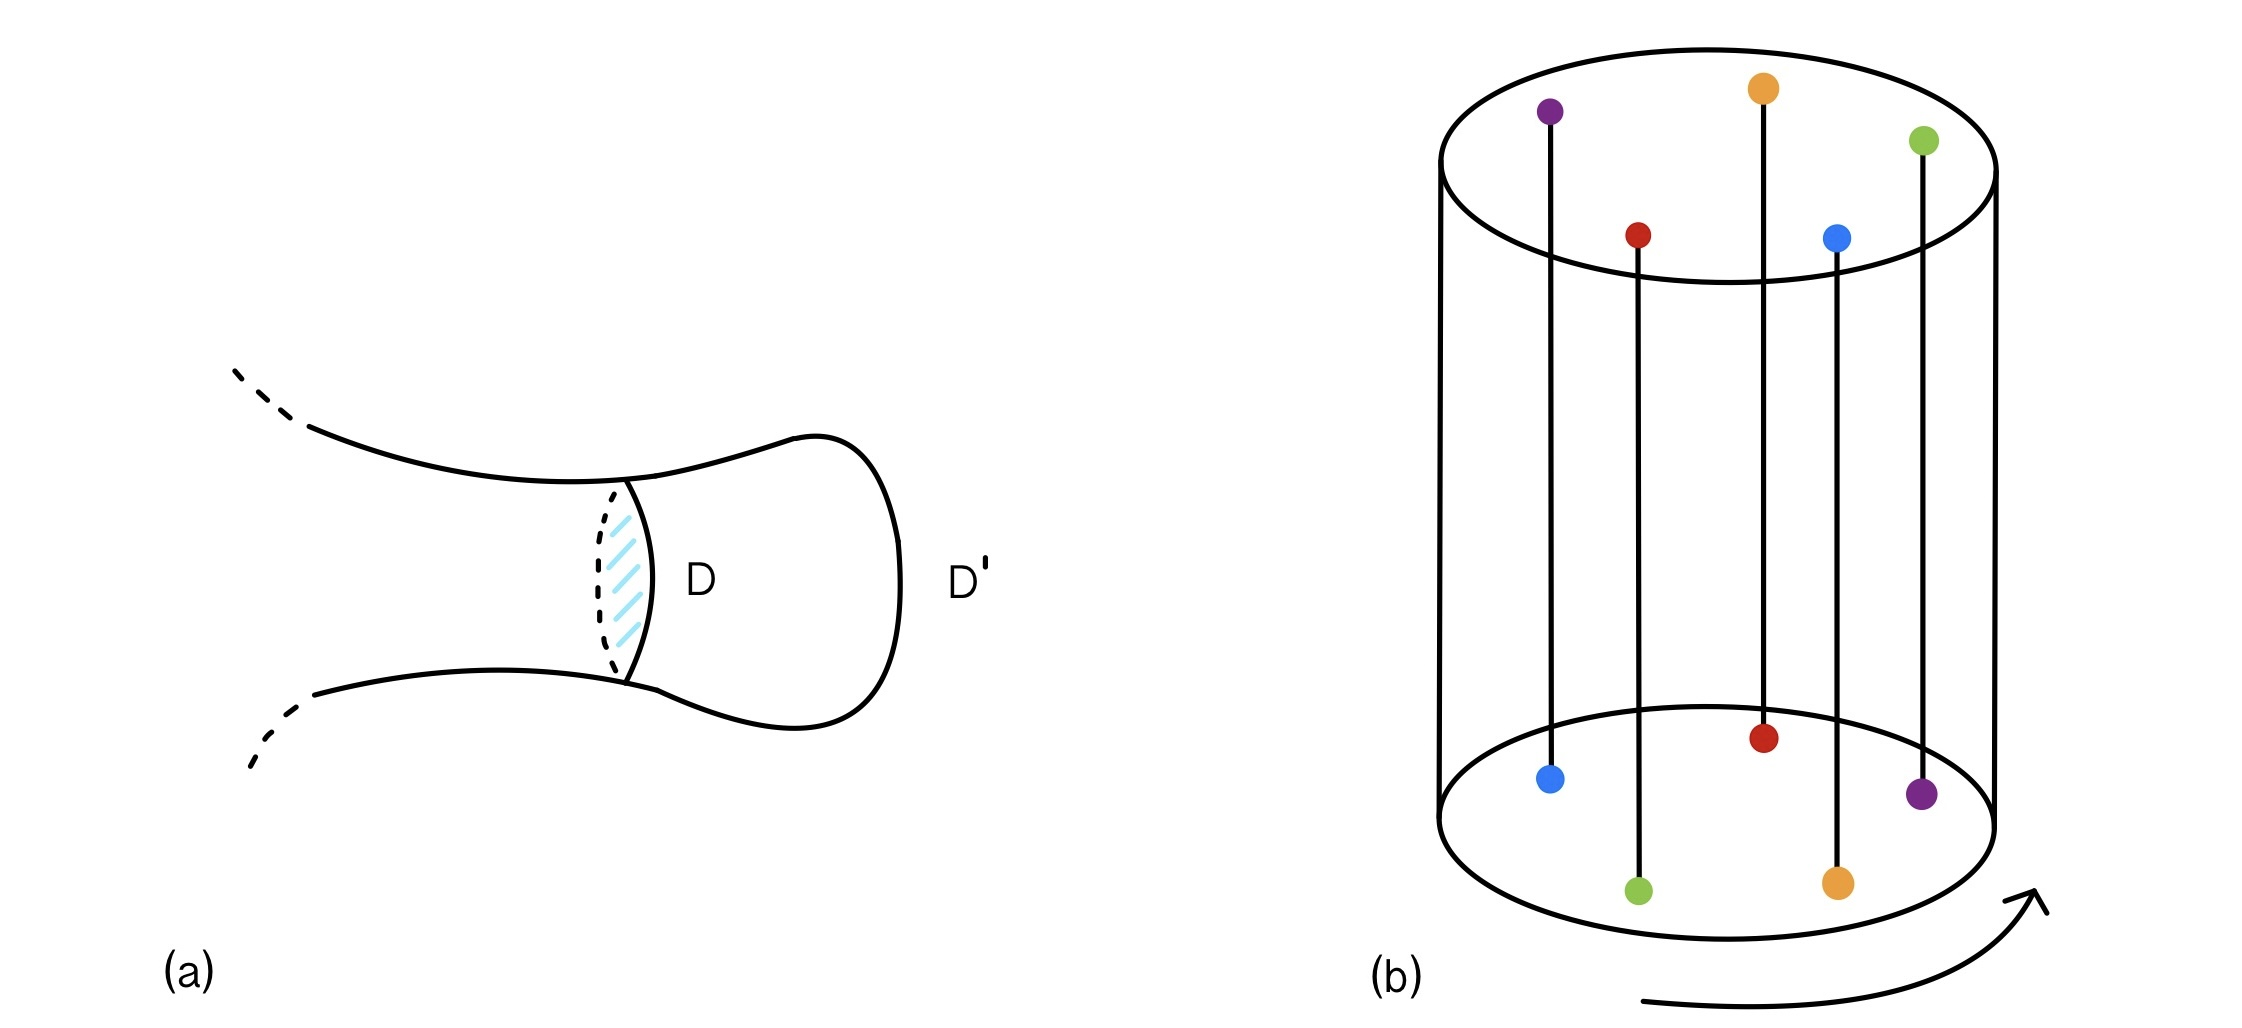
\includegraphics[scale=0.2]{figures/seifert.jpeg}
    \caption{An incompressible surface (a) and a Seifert fibered model of $\s^1 \times \D^2$ (b)}
    \label{fig:seifert}
\end{figure}
Now we describe the two building blocks for the decomposition. 
\begin{defn}Let $Y$ be an irreducible $3$ manifold. \\
(i) $Y$ is called atoroidal, if every incompressible torus $T^2 \rightarrow Y$
is isotopic to a component of $\partial Y$. \\
(ii) Let $p, q$ be coprime integers. A type $(p, q)$ model Seifert fibering of $\s^1 \times \D^2$ is a decomposition of $\s^1 \times \D^2$ into disjoint copies of $\s^1$ made as follow. We start with a cylinder $[0, 1] \times \D^2$ with fibers $[0, 1] \times \{x\} \quad x \in \D^2$. Then we glue the bottom $0 \times \D^2$ with the top $1 \times \D^2$ via a $\frac{2\pi p}{q}$ rotation (as in Figure \ref{fig:seifert}(b)). $Y$ is called Seifert fibered if it decomposes into disjoint copies of $\s^1$, and it is locally diffeomorphic to a model Seifert fibering of $\s^1 \times \D^2$. 
\end{defn}
\begin{ex}\label{sei1} The complement of a Hopf link $L$ in $\s^3$ admits a Seifert fibering. In fact, $\s^3 \setminus L \cong T^2 \times [0, 1]$.
\end{ex}
An important class of Seifert fibered $3$-manifolds are the complements of torus knots. 
\begin{prop}\label{sei2} Let $p\neq q$ be prime numbers. Then $\s^3 \setminus T_{p, q}$ admits a Seifert fibering.
\end{prop}
For a proof, consult \cite{martelli2016geometric} Proposition $11.2.5$. \\
Finally, we state the $JSJ$ decomposition theorem.
\begin{thm} \cite{jaco1978new}\cite{johannson1979homotopy}
Let $Y$ be a compact, irreducible, orientable $3$ manifold with toroidal boundary. Then $Y$ admits a minimal collection of disjoint, non-boundary parallel, incompressible tori $T = \{T_1, \dots T_k\}$, such that each component of $$
Y|T = Y \setminus (\nu(T_1)^{\mathrm{o}} \cup \dots \cup \nu(T_k)^{\mathrm{o}})
$$
is either atoroidal or Seifert fibered. Such collection is unique, up to isotopy. 
Moreover, for every diffeomorphism $\psi$ of $Y$, there exists a permutation $\sigma \in \mathfrak{S}_k$ such that $$
\psi(T_j) = T_{\sigma(j)}
$$
\end{thm}
With these tools in hand, we now prove Lemma \ref{techhh}. 
\proof Let $\varphi \in Diff(\s^3 \setminus K_m \# \torus)$.
We may view $K_m \# \torus$ as a satellite knot sitting inside $\nu(K_m)$. The torus $T = \partial \nu(K_m)$ is called a swallow-follow torus \ref{fig:swallow}(b), as it swallows $\torus$ and follows $K_m$ (which is depicted as a figure-eight knot for simplicity). Such torus is realized as the boundary of a component of $\s^3 \setminus (\nu(K_m) \cup S)$ (Figure \ref{fig:swallow}(a)), where $S$ is a decomposing sphere for $K_m \# \torus$. As discussed in Example \ref{heart}, $T$ is an incompressible torus in  $Y = \s^3 \setminus (K_m \# \torus)$. Thus we can decompose $Y$ along $T$ as: $$
(\s^3 \setminus \nu(K_m)) \cup_{\partial(\s^3 \setminus \mu) = T} (\s^3 \setminus \nu (\torus \cup \mu))
$$ 
where $\mu$ denotes a meridian\footnote{$\mu$ wraps around like $K_m$} of $\torus$. 
Similarly, $\s^3 \setminus (\torus \cup \mu)$ decomposes into two $JSJ$ pieces: $\s^3 \setminus \torus$ and the complement of a Hopf link. By Example \ref{sei1} and Proposition \ref{sei2}, the latter pieces are Seifert fibered, therefore they can't support a hyperbolic structure. Up to isotopy, we can assume that $\varphi(T) = T$, thus by uniqueness of the $JSJ$ decomposition, we conclude that $$
\varphi(\s^3 \setminus K_m) = \s^3 \setminus K_m
$$
Hence the thesis follows from Lemma \ref{technic}.
\endproof
\begin{figure}[H]
    \centering
    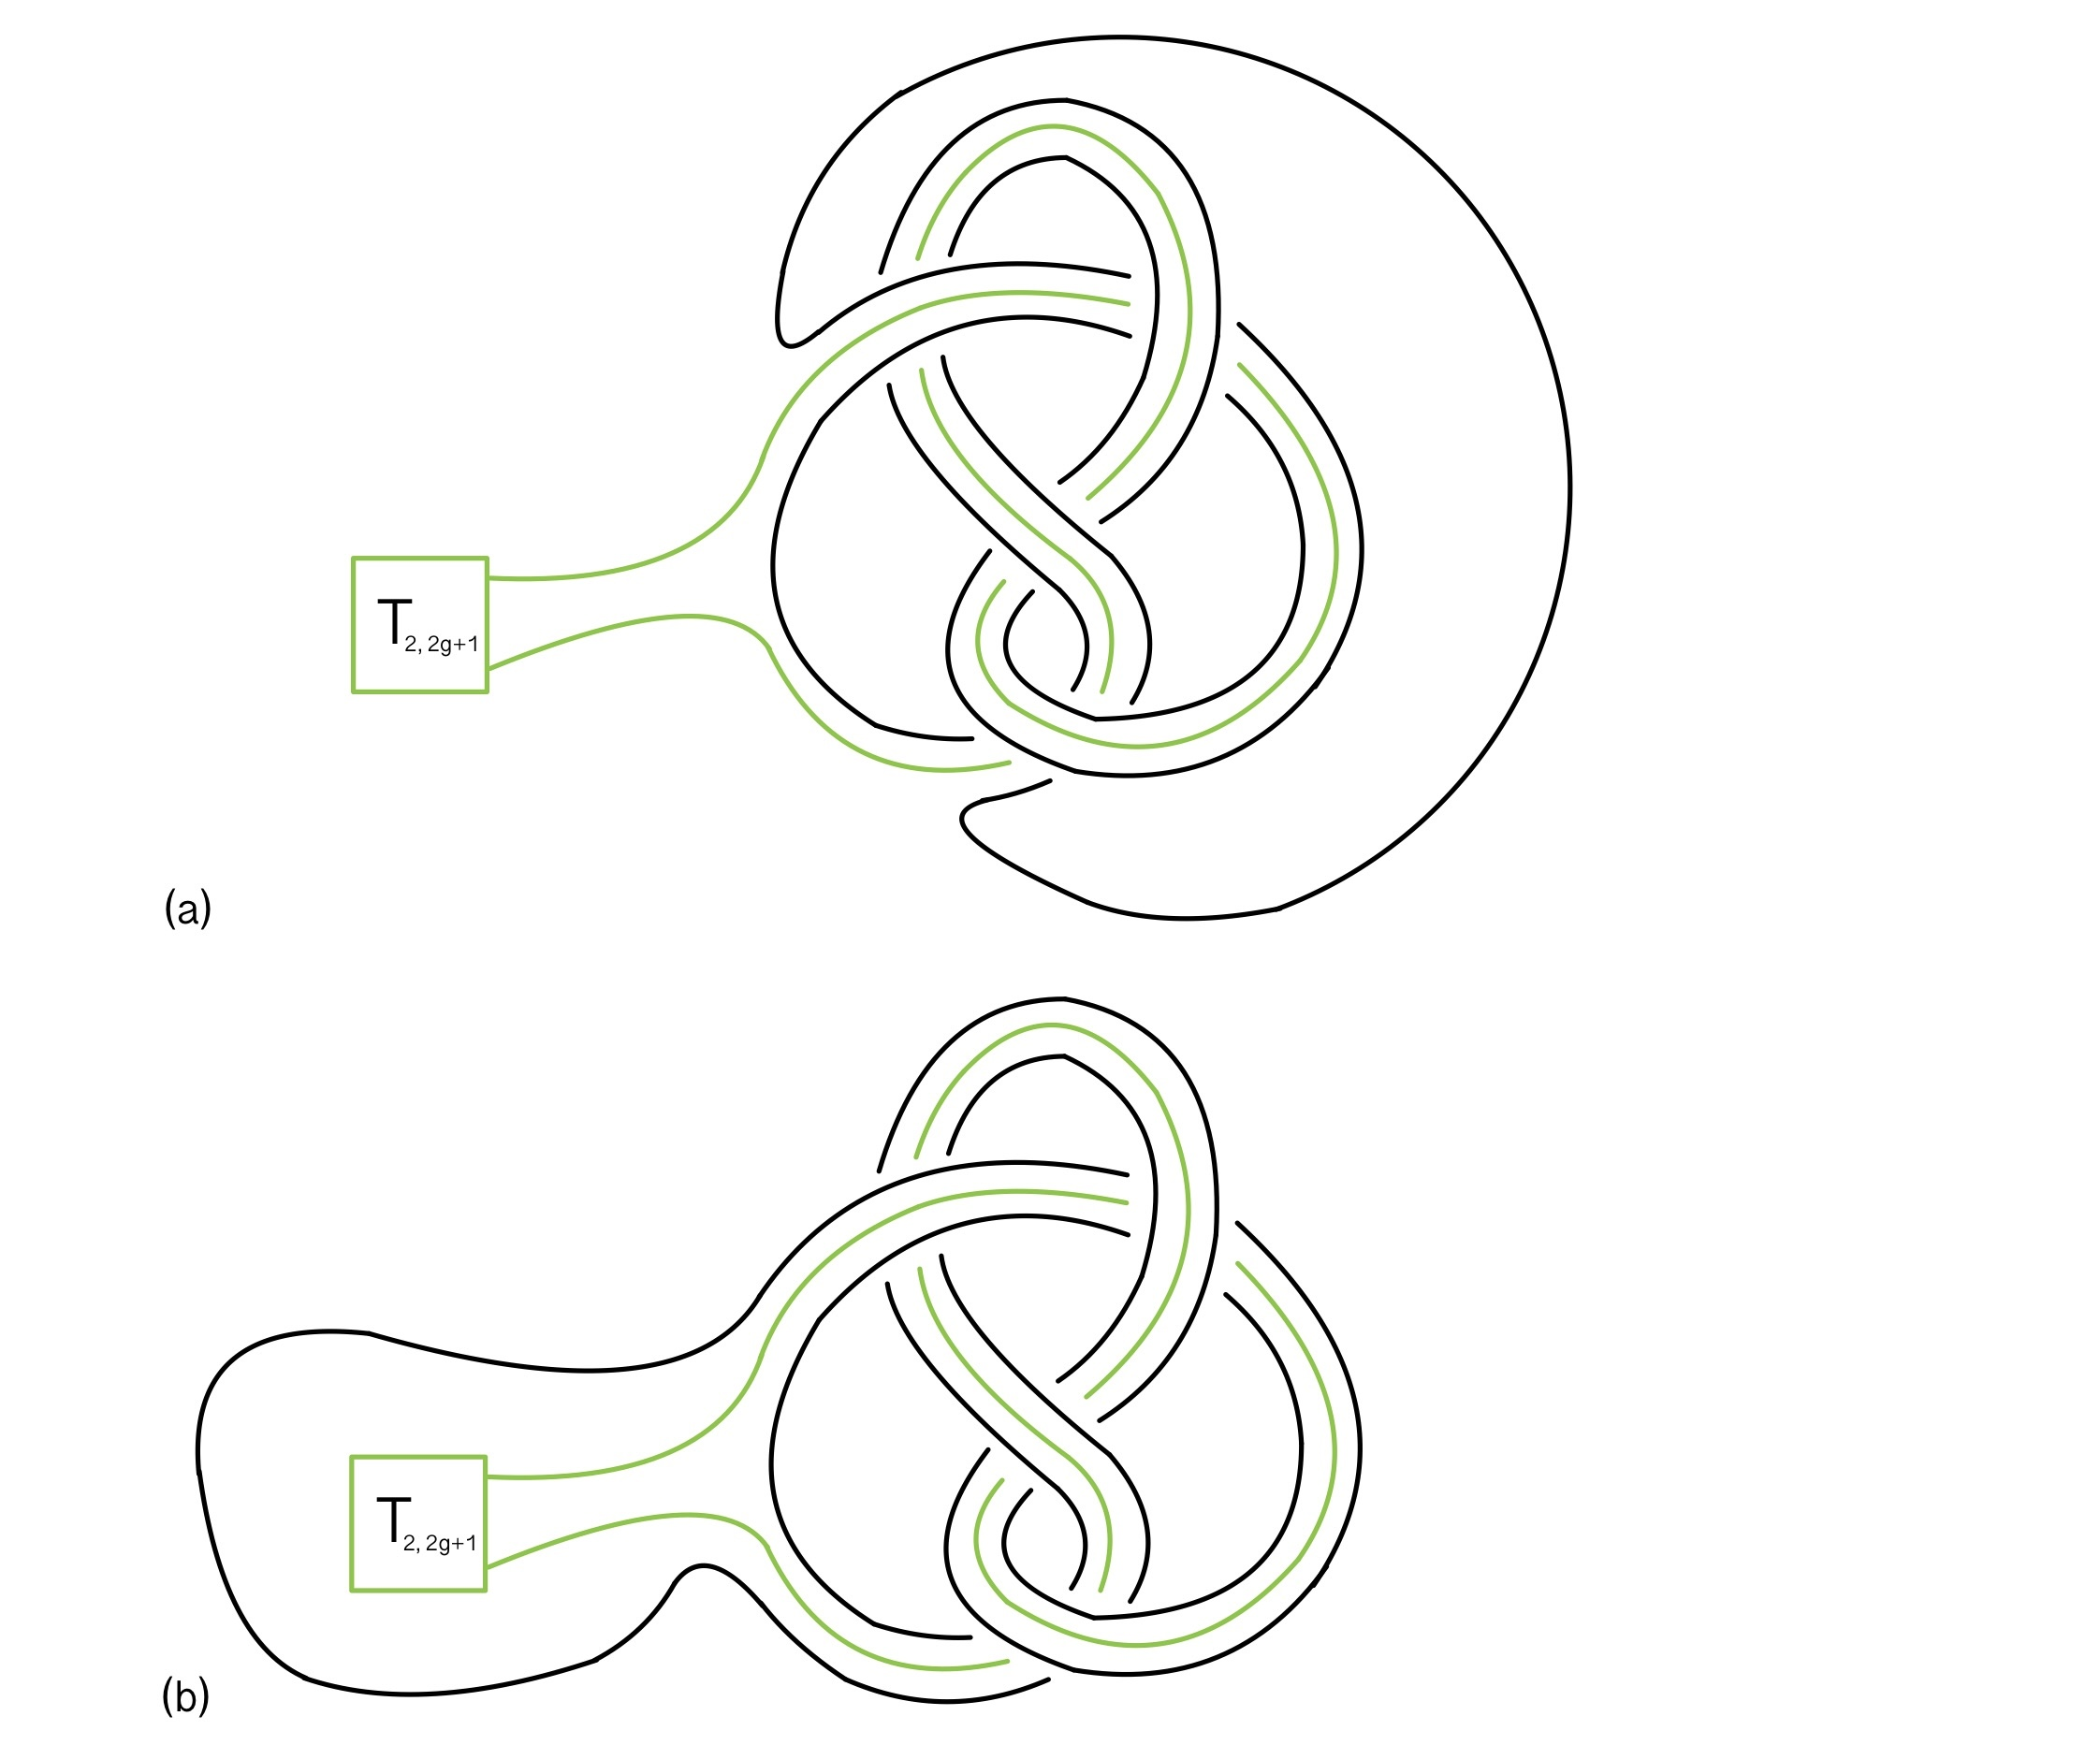
\includegraphics[scale=0.25]{figures/swallow.jpeg}
    \caption{A swallow-follow torus}
    \label{fig:swallow}
\end{figure}
As in the proof of \ref{prince}, $J$ bounds a disk $\mathfrak{D}'$ disjoint from $D'$.
By Lemma \ref{techhh} $$
\varphi(\mathfrak{D}') = \mathfrak{D} 
$$
is a disk bounded by $J$, which is contained in $\estd$.
Next, we aim to obstruct the existence of $\mathfrak{D}$, by analyzing a lift $\mathfrak{\tilde{D}}$ in the double branched cover $\Sigma(\B^4, F)$.
The existence and uniqueness of $\Sigma(\B^4, F)$ is proved in \cite{akbulutKirbyBranchedCovers}. The following Proposition ensures that $\Sigma(\B^4, F)$ is a Stein $4$-manifold.
\begin{prop}The following hold: \\
(i) $\Sigma(\B^4, D\natural F_0) = \Sigma(\B^4, D) \natural \Sigma(\B^4, F_0)$ \\
(ii) $\Sigma(\B^4, F_0)$ admits a Stein structure, \\
(iii) $\Sigma(\B^4, F)$ admits a Stein structure.
\end{prop}
\proof 
The first claim is straightforward from the definition of branched cover and the procedure to build it. \\
To prove (ii), we use the fact that a branched cover of $\B^4$ along an embedded holomorphic curve is analytic \cite{grauert_remmert_stein}. Then Theorem $3$ of \cite{loi_piergallini_stein} implies that $\Sigma(\B^4, F_0)$ is a Stein surface. \\
The last assertion follows from Gompf's standard form. In fact performing the connect sum corresponds to adding a $1$-handle.
\endproof
As the diagram of $\Sigma(\B^4, D)$ in Gompf's standard form is a portion of that of $\Sigma(\B^4, F)$, the final argument can be repeated verbatim. \\ \\
\section{Closed Case}
In this final section, we prove Theorem \ref{ulti}. As the proof is completely analogous to the proof of Theorem \ref{king}, we will only discuss the key changes. \\ \\
\proof
We consider $X_n = X_n(K \# \torus)$ as the ambient $4$-manifold. Let $G, G'$ be closed surfaces obtained by capping off $F, F'$ with the core of the $2$-handle in $X_n$. By Theorem \ref{hymn}, if $$
n \leq TB(K_m \# \torus)\footnote{This value is finite and does not depend from $m$ because $K_m$ has a Legendrian realization with $tb = -2$} - 1
$$

$X_n$ admits a convex symplectic structure. \\ Moreover, by Proposition \ref{tool4}, we can assume, up to isotopy, that $G, G'$ are symplectic in $X_n$. \\
It is straightforward to see that $G$ and $G'$ are topologically isotopic. \\
It remains to prove that they are not smoothly isotopic. Suppose, by contradiction, there exists $\varphi$, a self diffeomorphism of $\B^4$, such that $\varphi(G') = G$. \\
Next, we aim to show that $J \subseteq \partial X_n$ is fixed by $\varphi$, up to isotopy.
To this end, we prove an adapted version of Lemma \ref{tool8}, using again the $JSJ$ decomposition. 
\begin{lem} Let $n<<0$ and either $m<<0$ or $m=0$. Then every self diffeomorphism of $\partial X_n= \s^3_n(K_m \# \torus)$ restricts to the identity on $\s^3 \setminus \inter$, up to isotopy.
\end{lem}
\proof
First, we notice that $\partial \nu(K_m)$ defines an incompressible torus embedded in $\partial X_n$. Therefore $\s^3_n(K_m \# \torus)$ splits along $T$ into two $JSJ$ pieces, one of which is clearly $\s^3 \setminus K_m$. 
\begin{cla} The other piece is diffeomorphic to $\s^3 \setminus \torus$.
\end{cla}
In fact, the latter piece can be obtained by removing a meridian $\mu$ (of $\torus$) from $\s^3_n(\torus)$. Such meridian is glued to $n\mu+\lambda$ which is isotopic to $\torus$, the core of the surgered torus. \\
Thus $\partial X_n$ is decomposed as $$
\partial X_n|_T = (\s^3 \setminus K_m) \cup (\s^3 \setminus \torus)
$$
Recall that $\s^3 \setminus K_m$ is the only hyperbolic piece, as the other is Seifert fibered. Up to isotopy, every diffeomorphism of $\partial X$ preserves $T$ and restricts to a self-diffeomorphism of $\s^3 \setminus K_m$. Hence the thesis follows from Lemma \ref{technic}.
\endproof
Therefore $\varphi (\mathfrak{D'}) = \mathfrak{D}$ is a disk bounded by $J$ and disjoint from $G$. Next, we build the double branched cover of $X_n$ along $G$, using the same techniques employed in the proofs of Lemma \ref{warietto} and Theorem \ref{wario}. In particular, $$
\Sigma(X_n, G) = \Sigma(\B^4, F) \cup H_2
$$
with the $2$-handle attached along $\tilde{L}$, the lift of $K_m\# \torus$, with framing $\frac{n}{2}$. By Eliashberg's characterization theorem, if $$
n \leq TB(\tilde{L})-1
$$
$\Sigma(X_n, G)$ admits a Stein structure\footnote{As $n$ varies, using a sequence of negative stabilizations, we can always obtain a Legendrian realization of $\tilde{L}$ with $tb-1 = n$.}. From this point onward, the proof can be reproduced verbatim.
\endproof
\addcontentsline{toc}{chapter}{Appendix}
\chapter*{Appendix}\label{app}
The following Figure shows that purple band surgery (Figure \ref{fig:triv4}(p)) turns $K_m$ into two meridians for the red circle.
\begin{figure}[H]
    \centering
    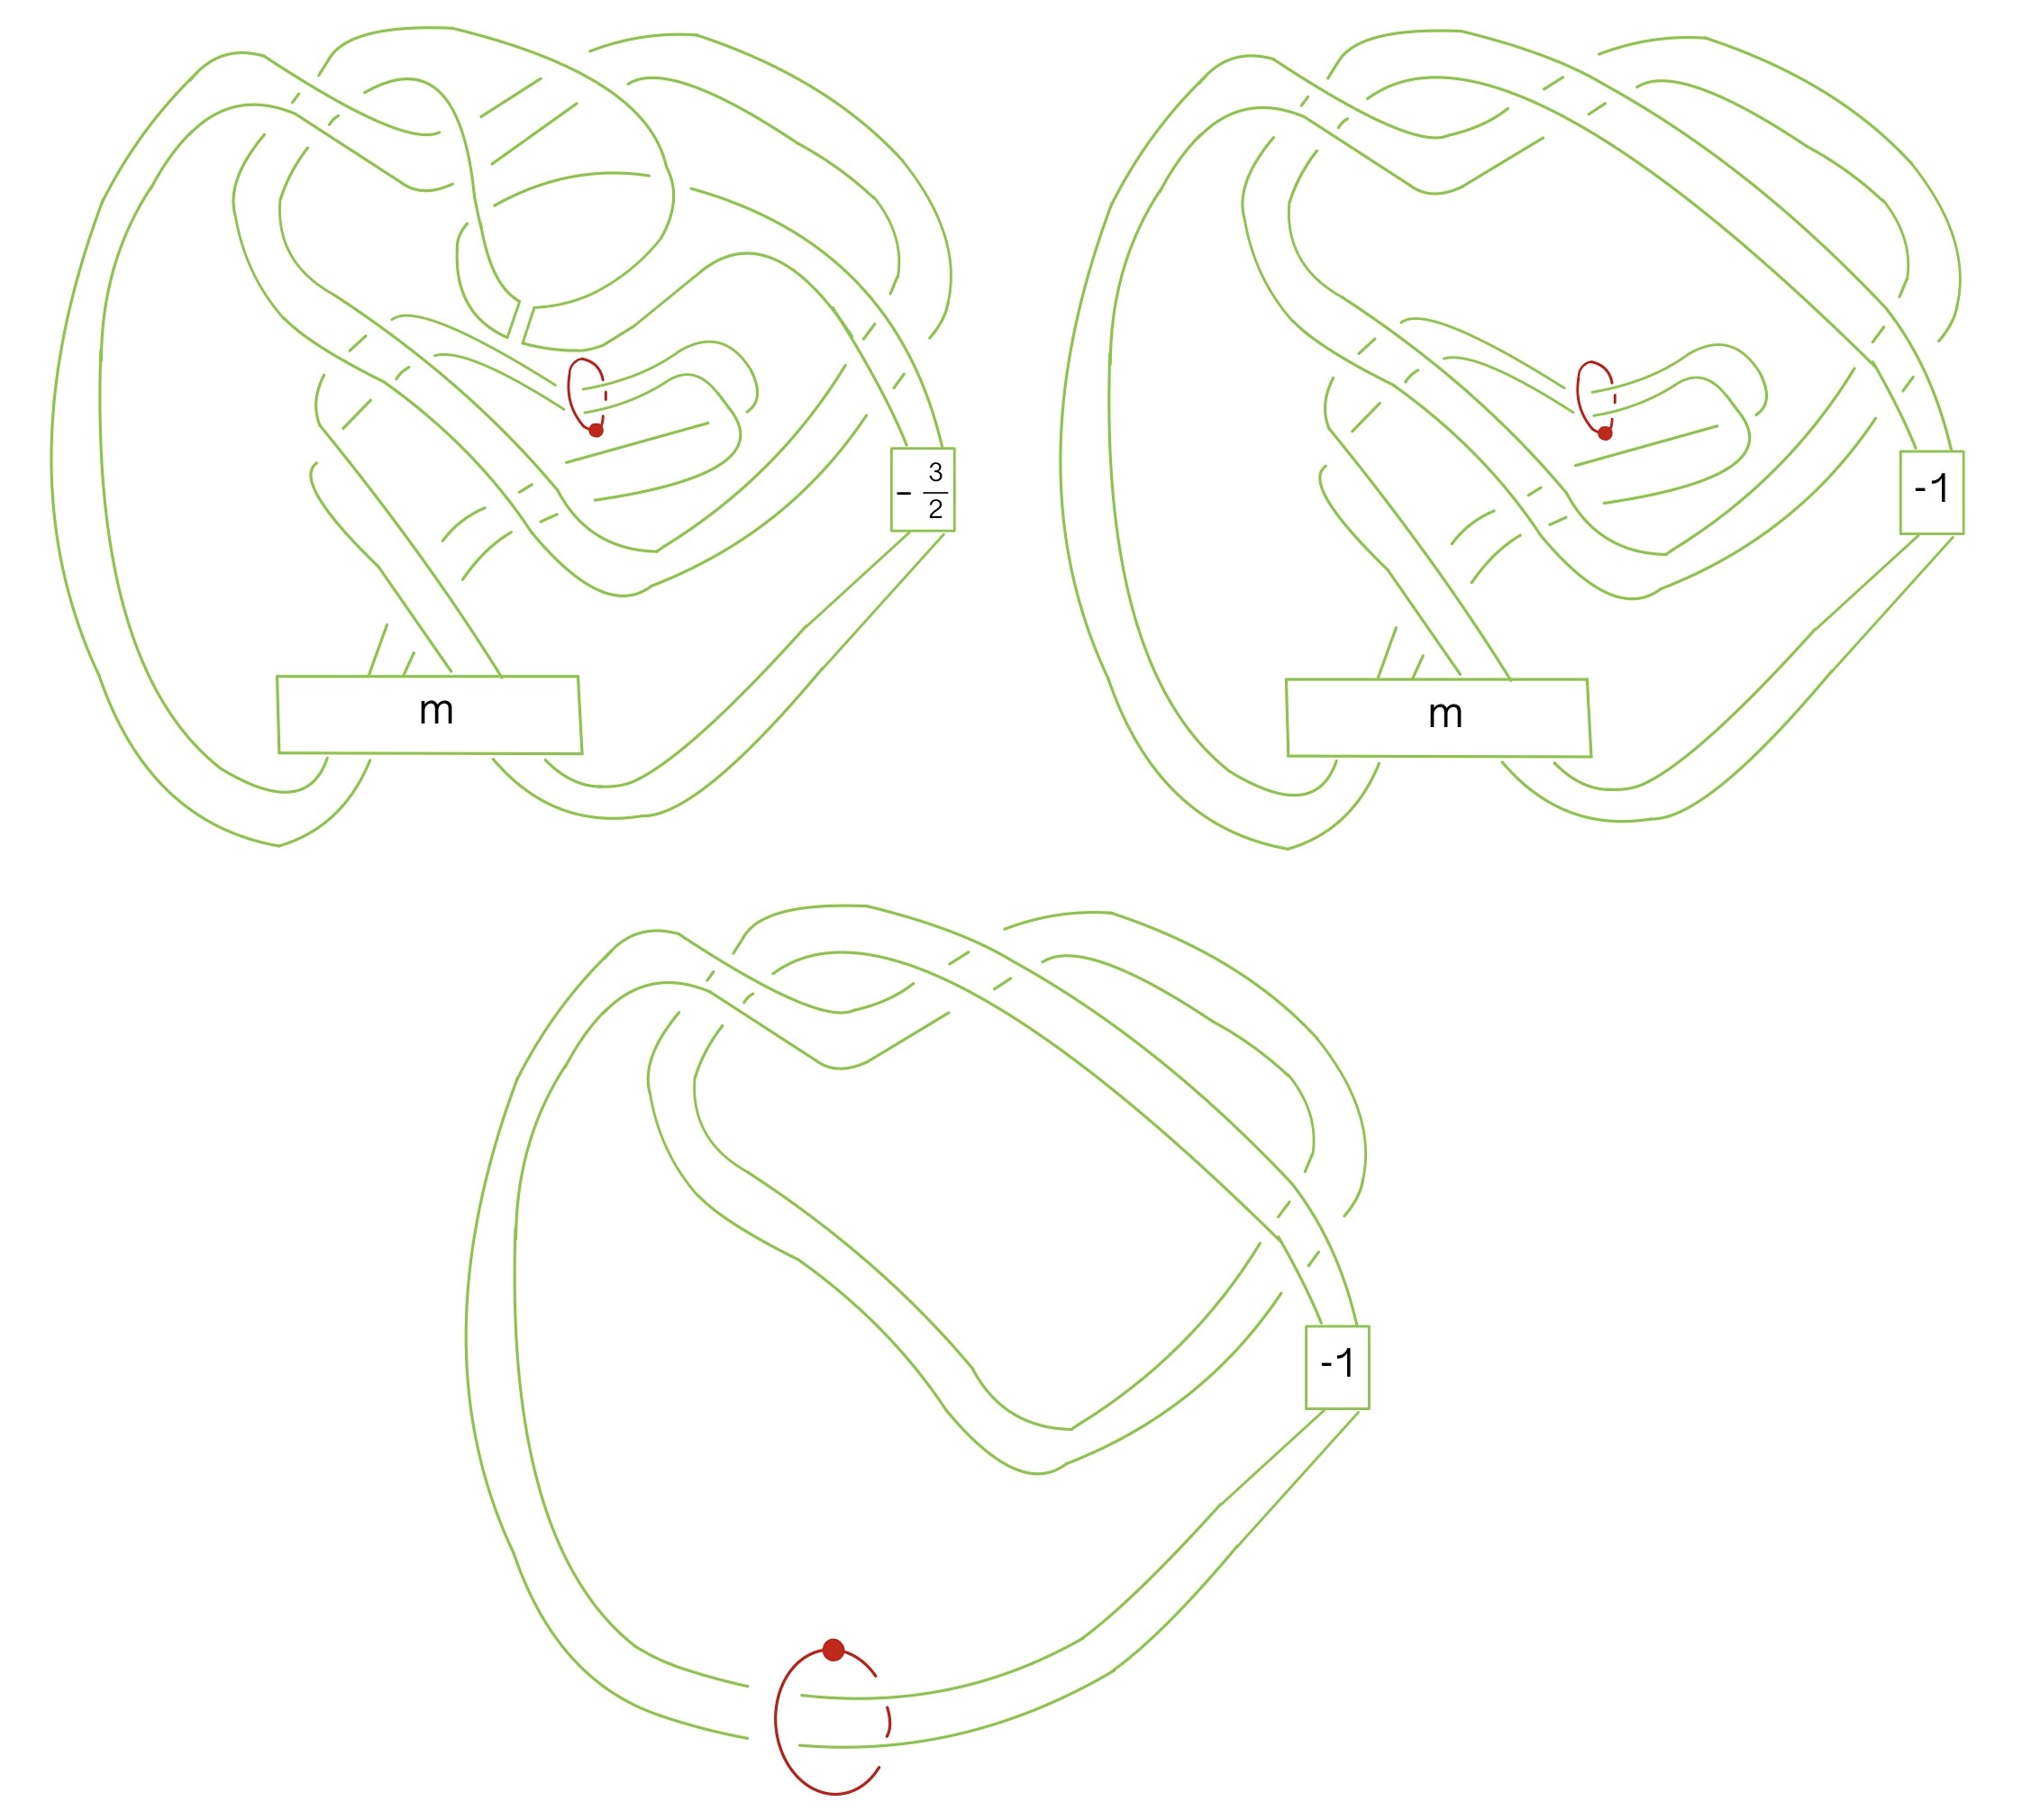
\includegraphics[scale=0.18]{figures/trade.jpeg}
    \caption{Purple band surgery}
    \label{fig:trade}
\end{figure}
\newpage
\textbf{Snappy Computation} \\ \\
We draw $K_m$ and $K_m \cup \gamma$ using KnotFolio\cite{knotfolio}, and we extract the Dowker-Thistlethwaite code. Then we run Snappy\cite{snappy} inside Sage\cite{sagemath}, in order to verify that $\s^3 \setminus K_0$ is hyperbolic and asymmetric. 
\begin{lstlisting}[language=Python]
import snappy 
In : K = snappy.Manifold('DT: [12, -64, 52, 20, -70, -30, -40, 2,
-28, -72, 34, -44, -54, -4, 62, 68, -58, 24, 76, -14, 66, 56, -22,
-32, 10, 18, -74, -36, 46, -8, -50, -16, 38, -78, -48, 60, -6, 26,
-42]')
K.solution_type()
Sage: 'all tetrahedra positively oriented'
In: K.verify_hyperbolicity()
Sage: (True,
 [0.93909513959? + 0.69095521566?*I,
  0.70707736232? + 0.93434842099?*I,
  1.52329395723? + 1.17752544467?*I,
  0.914749822027? + 0.628167321490?*I,
  -0.044422324121? + 0.404742729817?*I,
  -0.79978748449? + 0.31543544271?*I,
  1.124693783715? + 0.56925610185?*I,
  -0.05030425521? + 0.43711071362?*I,
  0.20238398208? + 0.45593871701?*I,
  1.086142103954? + 0.129177745136?*I,
  1.59150798543? + 0.64681487788?*I,
  0.34662975836? + 0.316285444394?*I,
  0.3682794911? + 12.5174820220?*I,
  0.83411890077? + 2.17547326363?*I,
  0.434120938316? + 0.486073861164?*I,
  0.58163452576? + 3.14286632765?*I,
  0.837518749600? + 0.430787981471?*I,
  -3.82632505439? + 4.30891057294?*I,
  0.51914091788? + 0.99861023843?*I,
  0.595092596715? + 0.409748194190?*I,
  0.78098699952? + 0.86961413751?*I,
  0.57918637538? + 0.94075132289?*I,
  0.363856100126? + 0.219817027992?*I])
In : R = K.canonical_retriangulation(verified = True)
In : len(R.isomorphisms_to(R))
Sage : 1 #this is the cardinality of the isometry group
\n \n
import snappy
In: Twocomponents= Link([(91,81,92,80), (81,89,82,88), 
(20,83,21,84), (13,43,14,42), (2,61,3,62), (27,63,28,62), 
(55,12,56,13), (84,19,85,20), (70,5,71,6), (9,83,10,82), 
(45,7,46,6), (85,11,86,10), (22,8,23,7), (31,19,32,18), 
(60,41,61,42), (14,73,15,74), (38,26,39,25), (86,30,1,29), 
(39,4,40,5), (76,4,77,3), (37,49,38,48), (71,59,72,58), 
(46,23,47,24), (43,17,44,16), (44,57,45,58), (69,25,70,24), 
(59,75,60,74), (30,11,31,12), (8,33,9,34), (1,55,2,54), 
(56,18,57,17), (77,26,78,27), (28,53,29,54), (72,15,73,16), 
(21,33,22,32), (79,67,80,66), (68,48,69,47), (78,49,79,50), 
(90,35,91,36),(52,64,53,63), (36,67,37,68), (92,65,93,66), 
(51,87,52,94), (93,51,94,50), (34,89,35,90), (64,87,65,88), 
(40,76,41,75)]) 
In: K = Twocomponents.exterior()
In: K.solution_type()
Sage: 'all tetrahedra positively oriented'
In : K.simmetry_group()
Sage: 0
\end{lstlisting}
\bibliography{references}
\addcontentsline{toc}{chapter}{Bibliography}

\bibliographystyle{alpha}

\cleardoublepage
\listoffigures
\addcontentsline{toc}{chapter}{List of figures}

\end{document}
    